\documentclass[12pt,authoryear, notitlepage]{elegantpaper} 

\usepackage[figuresright]{rotating}
\usepackage{hyperref}
\usepackage{adjustbox}   %% you can resize if the table goes beyond \textwidth
\usepackage{graphicx}
\usepackage{pdfpages}
\usepackage{dirtytalk}
\usepackage{amsmath}
\usepackage{geometry}
\geometry{a4paper, margin=1in}
\usepackage{tikz}
\usetikzlibrary{arrows.meta, positioning}

\usepackage{xpatch}
    \newlength{\chaptertopskip}
    \setlength{\chaptertopskip}{10pt}
    \makeatletter
    \xpatchcmd{\@makechapterhead}{\vspace*{50\p@}}{\vspace*{\chaptertopskip}}{\typeout{Success}}{\typeout{Failure!!!}}
\makeatother
\usepackage{dialogue}
    % redefine dialogue environment to use new parameters
    \makeatletter
    \renewenvironment{dialogue} {%
        \begin{list}{} {%
            \setlength\itemsep{\z@ \@plus .5ex}%
            \setlength{\parsep}{\parskip}%
            \setlength{\rightmargin}{0pt}% no indentation on right; change this if you wish
            \setlength{\labelsep}{0.5em}% space between (longest) name and text
            \setlength{\leftmargin}{\labelwidth}% set margin on left to same width
            \addtolength{\leftmargin}{\labelsep}% plus the label sep
            \defcommand\speak[2]{\item[\hfill {##1}] {\itshape ``{##2}''}} % define speak command
            \let\makelabel\DialogueLabel
          }%
          \PreDialogue\relax
        }{%
      \end{list}%
      }
    \makeatother
\usepackage[caption=false]{subfig}
\usepackage{subfiles} % Best loaded last in the preamble
\usepackage{natbib}
\usepackage{diagbox}
\usepackage[figuresright]{rotating}
\usepackage{threeparttable}
\usepackage{multirow}
\usepackage{bbm}
\usepackage{url}
\usepackage{lipsum}
\usepackage{setspace}
    \footnotesep=10pt
    \usepackage{etoolbox}
    \makeatletter
    \patchcmd{\@footnotetext}
      {\setspace@singlespace}{0.8}
      {}{}
    \makeatother % 调整footnote的行间距
    

\renewcommand{\baselinestretch}{1.8} % 调整行间距
\DeclareRobustCommand{\firstsecond}[2]{#1}



\title{Time-Varying Oligopsonistic Competition, Storage Dynamics, and Welfare in Agricultural Markets}
\author{Zhiyao (Yao) Ma}
\institute{Committee: Richard J. Sexton, Jeffrey C. Williams, and Stephen Boucher}
\date{\today}

%----------------------------------------------------------------%
%----------------------------------------------------------------%

\begin{document}
\maketitle
\thispagestyle{empty}


\begin{dedication}
\textit{For my beloved grandparents}\\
\textit{Qilong Ma, Qingzhen Fei, Qingxiang Li, and Yanling Sun}\\
\textit{whose love and guidance endure in memory.}
\end{dedication}


\newpage
\pagenumbering{roman}


\begin{acknowledgments}
This journey has been extraordinary, and the gratitude I feel for those who supported me along the way is beyond what words can convey, though I will do my best. I am deeply indebted to my advisors, Richard J. Sexton and Jeffrey C. Williams, for their invaluable guidance and extraordinary mentorship. Richard's clarity of thought, insistence on careful identification, and instinct for policy-relevant questions shaped every chapter of this dissertation. He taught me how to connect theory to institutions and data, to write both parsimoniously and elegantly, and to defend ideas with evidence rather than volume. Jeffrey has been a gold mine of insight: whenever I became tangled in brainstorming or modeling, he helped me tango on with balance and rigor. Our explorations of commodity futures markets and storage dynamics in U.S. and Chinese supply chains will remain a lasting source of inspiration. I aspire one day to grow into someone with their vitality, charisma, and intellectual power.

I am grateful to Stephen Boucher, who served on my dissertation committee and provided valuable input from the very beginning of my journey. I will never forget the Zoom moment when I received the acceptance, nor the many hours Steve and I spent together refining my fieldwork plan in detail. I also owe special thanks to Professor Michael R. Carter for his insightful comments and suggestions on this research---whether in the classroom, during the development sequence, or over a glass of wine in beautiful Sonoma County. Every presentation of his was a pure joy and inspired me to think more deeply about ongoing development issues.

This research has also benefited immensely from feedback received from UC Davis faculty, like Colin Carter, Rachael Goodhue, Ashish Shenoy, Diana Moreira, Katrina Jessoe, Pierre M\'erel, and Matthew Reimer. I am equally grateful to the outstanding graduate students and alumni from the ARE and Economics departments---Shisham Adhikari, Mohan Chen, Matthew Dudek, Yan Ge, Jiawei Guo, Rachel E. Jones, Gal Koss, Gilberto Jose Nogueira, Zhiran Qin, Hui Ren, Yujing Song, Qi Wu, Shuhan Zeng, and Jiahao Zhu---whose suggestions, critiques, and encouragement were invaluable. I also thank my department as a whole for providing the unique opportunity to pursue this degree and to grow both as a scholar and as a person.

A special thanks goes to the apple growers and local officials in Yanchang County, Shaanxi Province, China, where I conducted my fieldwork, for generously providing information that inspired much of this research. I am also fortunate to have had opportunities to consult with officials, both junior and senior, from the China Securities Regulatory Commission, the China Zhengzhou Commodity Exchange, and the China Financial Futures Exchange. Their insightful observations and probing questions motivated me to carry on and to contribute, in a small way, to real-world solutions.

Most heartfelt thanks go to my family for their love and support. I am blessed with the greatest parents, Wei Ma and Xuesong Li, who shaped my character and encouraged me to explore the world. I am profoundly grateful to my fianc\'ee, Yining Xiang, who has been a constant source of inspiration since our undergraduate years. She contributed research ideas, helped with fieldwork, and engaged in countless helpful discussions. I know that her love, patience, and sacrifices sustained my well-being and made it possible to complete this dissertation.

I am also fortunate to have great friends---Yuanshang Ding, Kefan Guo, Ziheng Hua, Mengjiang Huang, Ye Hong, Ziqiang Liu, Qizhen Liu, Xin Lan, Fenglin Lu, Zhongxian Ren, Lingxiao Qian, Changgeng Xu, Jing Xu, Yan Xu, Yuanruo Xu, Yingeng Zhang, Chang Zhang, Guyu Zhang, Duanduan Zhu, and Hui Zhu---who offered unconditional help and camaraderie beyond academic pursuits.

Finally, I would like to thank the many researchers I met at academic conferences, including the 2025 AAEA Annual Meeting, who provided constructive suggestions on this work. All remaining errors in this dissertation are, of course, my own.
\end{acknowledgments}




\newpage
\begin{abstract}
This dissertation reframes oligopsonistic power in agricultural procurement as time-varying rather than fixed, showing how buyer competition waxes and wanes within a single marketing season and how farmers use storage to shift when, and on what terms, they sell. Using China's fresh-apple sector as the empirical setting, I argue that storage is not only a vehicle for intertemporal arbitrage but a lever that reallocates relative power toward smallholders when oligopsony conditions loosen over time.

I build a two-period model in which buyer power is time-varying and farmers equipped with storage can optimally ``wait into'' possibly more competitive windows. The framework cleanly separates buyer-power dynamics from demand shocks and illuminates how expectations about the future competitive conditions among rivalry and risk preferences jointly determine storage choices and realized selling conditions. Numerical simulations with heterogeneous risk preferences map storage efficiency and risk attitudes to welfare, quantifying when waiting pays, how risk aversion suppresses storage, and why policies that raise storage efficiency or reduce effective risk aversion lift certainty equivalents and mean incomes. Equal-sized storage subsidies yield uneven benefits: when existing storage costs are high, they function like insurance; when storage is already affordable, they amplify farmers' returns like a growth multiplier.

Empirically, a field survey of over 500 apple growers in an interior region in central China tracks trading timelines, subjective expectations of buyer competition, objective measures of buyer competitiveness, and storage access. Storage adoption and time-to-sale respond strongly to anticipated future rivalry and logistical frictions, closely matching the model's predictions. Policy-wise, the results point beyond price supports toward market design: strengthen buyer competition at any point in the season, upgrade storage efficiency, and expand credit or insurance, each margin raises welfare without directly interfering with market prices.
\end{abstract}




\setcounter{tocdepth}{2}

\tableofcontents
\addcontentsline{toc}{chapter}{List of Figures}
\listoffigures
\addcontentsline{toc}{chapter}{List of Tables}
\listoftables


%----------------------------------------------------------------%
%----------------------------------------------------------------%

% Switch to arabic page numbering starting at Chapter 1
\clearpage
\pagenumbering{arabic}

\newpage
\chapter{Introduction} \label{Chapter: introduction}
    

\noindent
Buyer power has long been a central concern in agricultural economics, yet much of the literature treats it as a \textit{static} phenomenon---fixed, predictable, and structurally embedded. Classical and neoclassical models, rooted in industrial organization theory, often portray buyer power as a durable feature of market structure, shaped by concentration ratios, economies of scale, or long-term strategic behavior among firms \citep{sexton2013market}. In these frameworks, power is held by entities that are large, formally organized, and largely immune to short-run shocks or spatial variability \citep{sexton2010grocery}.

However, this perspective is increasingly insufficient, especially in the context of agricultural procurement systems in developing economies. These systems are defined not by structural rigidity, but by institutional informality, infrastructural gaps, and temporal volatility \citep{barrett2008agricultural}. Smallholder farmers in these settings interact with procurement markets that are seasonal, fragmented, and frequently unstable \citep{wang2020transaction}. Trader entry, buyer behavior, and market concentration fluctuate across space and time \citep{fafchamps2005selling, sitko2014exploitative, bergquist_dinerstein_2020}. As a result, the practical distribution of market power is both diffuse and dynamic.

This dissertation proposes a fundamentally different lens: market power in agricultural procurement is not merely a function of concentration, it is also dynamic, time-varying, and deeply contingent on local and temporal conditions \citep{barrett2022agri}. Drawing on rich empirical evidence from China's fresh apple industry---the world's largest by production volume---I explore how buyer competition fluctuates intra-seasonally; how farmers respond to this volatility through strategic use of cold storage; and how storage access, in turn, can reshape the very structure of buyer power. At the heart of this inquiry is a novel argument: storage is not only a vehicle for price arbitrage \citep{burke2019sell, wright1982econ}, but also a strategic tool for intertemporal bargaining amid a dynamic environment for market competition.



\paragraph{The Fragility and Fluidity of Buyer Power.}
The common belief that more buyers equate to more competition is challenged by detailed fieldwork in Yanchang County, Shaanxi Province. In this setting, oligopsonistic behavior is widespread, yet highly unstable. Farmers encounter procurement environments that change from month to month, and even week to week, with no clear patterns of predictability. This time-variability of buyer power stems from three interrelated economic mechanisms:
\begin{enumerate}
    \item \textbf{The Fragile Nature of Collusion}: Informal buyer cartels often emerge in local markets, particularly during the narrow window of post-harvest trade. These interest groups rely on tacit collusion, facilitated by WeChat groups, repeat interactions, and informal market territories, to suppress competition and discipline prices \citep{macchiavello2015value}. However, these arrangements are inherently fragile. They can collapse under the weight of defection, local disputes, or price pressures from downstream buyers. The absence of formal enforcement mechanisms makes them vulnerable to short-run shocks and opportunistic behavior.

    \item \textbf{Capacity Constraints and Randomized Access}: Traders operate under tight logistical and capital constraints \citep{ambler2023finance}. Their truck fleets, cold storage facilities, and downstream distribution agreements are limited, and not all procurement opportunities are equally viable. As a result, trader entry into any given village to procure product is somewhat stochastic. Some villages may see a glut of buyers competing vigorously, while others may be visited by only one, creating effective monopsony conditions. From the farmer's perspective, this randomness translates into a procurement environment that is unpredictable and unbalanced in terms of competitive conditions.

    \item \textbf{Territoriality and the Threat of Outside Entry}: Many local trader networks establish de facto procurement territories through informal agreements to avoid internal competition. However, these agreements are fragile. Non-local traders, who often arrive with fewer relational constraints and larger operational scales, pose a constant threat of disruption. Their entry can undermine local collusion, drive price competition, and redistribute bargaining power \citep{BARTKUS2022}. Yet their presence is also highly seasonal and uneven, adding another layer of temporal volatility to the procurement structure.
\end{enumerate}

\noindent
Together, these mechanisms generate a procurement landscape where market power is not a fixed feature of the supply chain, but a dynamic phenomenon. Villages may move into and out of competitive and collusive phases. Buyers switch roles between colluding partners and price competitors. Farmers, in turn, must navigate this evolving terrain with limited information and weak institutional support.

This dissertation is the first to formally model and empirically document this dynamic, and to consider its implications not just for price formation, but for the intertemporal strategies that farmers equipped with storage can use to benefit in the face of uncertainty.


\paragraph{Storage as a Strategic Bridge Across Competitive Periods.}
In agricultural markets for storable or semi-storable commodities, the temporal variability of buyer competition creates a distinctive incentive structure. Unlike perishable crops, which must be sold within days of harvest, storable crops like apples enable farmers who can access storage to choose when to sell. This choice mediated by storage opens up new strategic pathways.

Farmers who store in essence obtain multiple ``draws'' from the distribution of competitive market conditions over time. If the immediate post-harvest period is characterized by collusion or monopsony, storage allows farmers to delay sales in expectation of obtaining a more favorable buyer environment in the future.

In this sense, storage is not merely an inventory management tool \citep{goyal2010information}, it is a mechanism for intertemporal bargaining. It creates a form of market power for the farmer, shifting the dynamics of the negotiation. Once product is in storage, the immediate imperative to sell disappears. The seller gains time, options, and leverage. Buyers, in contrast, must compete in a broader, more centralized marketplace.

Indeed, cold storage facilities often function as de facto terminal markets. They aggregate supply from multiple growers, attract buyers from broader regions, and facilitate more transparent and competitive pricing. Traders converge on storage hubs rather than individual villages, and in doing so, must compete more directly with one another. This reshapes the power dynamics of the supply chain and creates a temporary re-balancing in favor of producers, especially those with access to high-quality, low-cost storage. The very act of storing thus transforms not only the timing of transactions, but also the structure of the procurement market itself.


\paragraph{Intertemporal Marketing and the New Storage Economy.}
By jointly analyzing storage decisions and buyer competition, this dissertation challenges conventional wisdom about farmer behavior. The prevailing narrative holds that farmers store to capture expected price increases arising from seasonal demand shifts. While this is true in part, the field data reveal an alternative rationale: farmers may store to escape weak bargaining conditions, hedge against collusion, and access more competitive markets.

This reframing of the rationale for storage has several important implications:

\begin{itemize}
    \item \textbf{First}, it expands the welfare narrative around storage. Storage does not only enable price smoothing or loss reduction, it serves as a strategic tool to avoid monopsony pricing and access different competitive environments over time. 

    \item \textbf{Second}, it explains why inefficient or high-cost storage is widely used. Even when the financial returns from arbitrage are marginal or negative, the non-monetary value of avoiding exploitative procurement periods may still justify the decision. In other words, storage has a strategic payoff, even in the absence of direct profits \citep{suri2011selection}.

    \item \textbf{Third}, it underscores the institutional frictions that limit storage access---especially for poor or liquidity-constrained farmers. Since the gains from storage accrue disproportionately to those who can afford it, unequal access to storage may exacerbate rural inequality and entrench disadvantage. Conversely, well-designed interventions, such as cold storage subsidies or cooperative storage networks, can have disproportionately positive effects on farmer welfare and market efficiency.
\end{itemize}

\paragraph{A New Lens on Agricultural Market Power.}
This dissertation makes three core contributions to the study of agricultural market dynamics:

\begin{enumerate}
    \item \textbf{Conceptual}: It develops a two-period dynamic model of time-varying oligopsony in agricultural procurement, integrating temporal shifts in buyer competition and endogenous farmer storage decisions. The model departs from traditional static IO frameworks by incorporating time-vary oligopsonistic power across periods.

    \item \textbf{Empirical}: It draws on original field data, including over 500 interviews and surveys with farmers, traders, and storage operators, to document the temporal variability of market structure, the strategic logic of storage, and the welfare impacts of intertemporal marketing choices.

    \item \textbf{Policy Relevance}: It offers a novel economic justification for investments in cold chain infrastructure and market design. By reframing storage as a lever for redistributing bargaining power, the findings suggest that targeted storage subsidies, improvements in farmer access to commercial storage, and reductions in transaction frictions could serve as powerful tools for enhancing both efficiency and equity in agricultural markets.
\end{enumerate}


\paragraph{Structure of the Dissertation.}
The chapters that follow elaborate on these themes using both theoretical and empirical approaches.

\begin{itemize}
    \item \textbf{Chapter 2} provides an institutional and empirical overview of China's apple industry, with a focus on storage practices, upstream buyer structure, and the field-level evidence on collusion and entry.

    \item \textbf{Chapter 3} reviews the literature on storage economics, market power in agriculture, and smallholder marketing under uncertainty, identifying critical gaps this dissertation seeks to fill.

    \item \textbf{Chapter 4} presents a dynamic two-period model of time-varying oligopsony and storage adoption, analyzing both individual farmer decisions and aggregate welfare implications under different scenarios of buyer behavior and risk preferences.

    \item \textbf{Chapter 5} empirically tests key predictions using survey data and interviews from Yanchang County. It explores the determinants of storage adoption, the relationship between buyer competition and timing of sales, and the welfare impacts of storage under constrained competitive environments.

    \item The appendices contain mathematical derivations, additional robustness checks, and the survey instruments used in fieldwork.
\end{itemize}




%----------------------------------------------------------------%
%----------------------------------------------------------------%
\newpage
\chapter{Oligopsony, Storage Inefficiency, and Welfare in China's Apple Industry}
\label{Chapter: descriptive chapter}

\begin{abstract}
This chapter addresses three key questions:
\begin{enumerate}
    \item What does the fresh apple industry look like in China?
    \item How does upstream buyer power influence the supply chain?
    \item Why does inefficiency persist in the storage process?
\end{enumerate}
\end{abstract}

    
%----------------------------------------------------------------%
%----------------------------------------------------------------%
\newpage
\section{Overview of Fresh Apple Industry}
\noindent This section provides an overview of China's fresh apple industry, covering production, consumption, import-export, supply chain dynamics, the role of storage, and the fresh-apple futures market. National-level analyses will be paired with insights from fieldwork in Yanchang County, Shaanxi Province, to offer a grounded perspective on industry trends and practices.

\subsection{Production, Consumption, and Import-Export}
\noindent While China's apple market may not be fully autarkic, it is largely domestically oriented, with limited reliance on foreign supply or demand.

\subsubsection{The Dominant Producer with Huge Domestic Consumption}
\noindent China's apple industry stands as the largest in the world, with the country consistently accounting for more than half of global apple production from the 1990s onward. As shown in Figure~\ref{fig: production quantity}, China's apple production has expanded steadily in recent decades, supported by the emergence of both large-scale farming operations and a vast number of small and medium-sized growers switching to apple cultivation. The availability of abundant land and a favorable climate for apple cultivation, particularly in provinces like Shaanxi, Shandong, and Henan, has allowed China to maintain its dominant position in the sector \citep{sun2021production}.


\begin{figure}[hpt]
    \centering
        \caption{Fresh-Apple Production Quantities in China, US, and Worldwide from 1961 to 2023}
    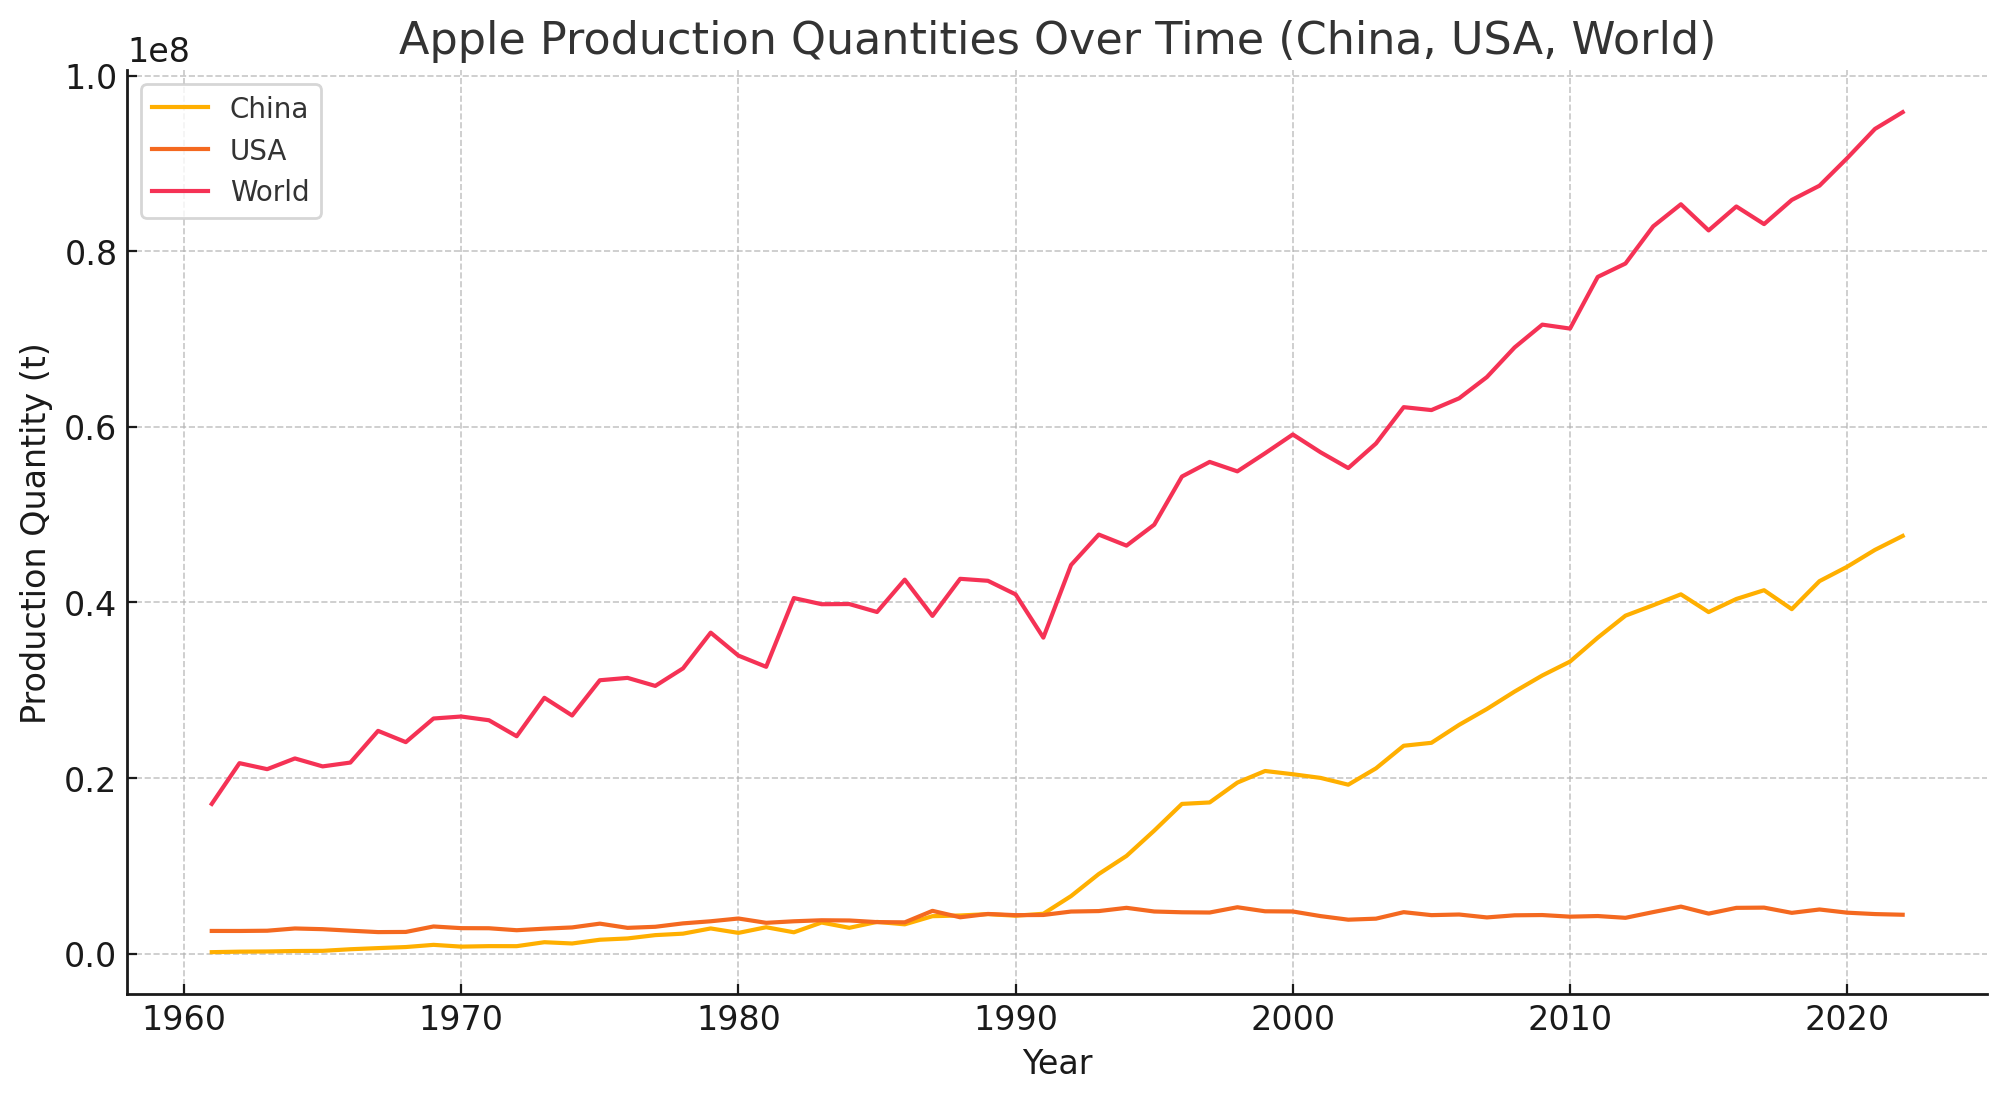
\includegraphics[width=\linewidth]{figures/production_China_US_world.png}
    \label{fig: production quantity}
    \begin{tablenotes}
    \footnotesize
    \item Source: The Food and Agriculture Organization Statistical Database (FAOSTAT)
    \end{tablenotes}
\end{figure}

The rapid development of the apple industry over the past few decades in China has resulted in a dramatic increase in farmers' incomes in low-income regions of the country. Since the Reform and Opening-up policy, apples have been at the forefront of market-oriented reforms. It was also among the first batch of agricultural products that China planned to fully liberalize in the 1980s. This early liberalization paved the way for more market-driven pricing and production decisions, which spurred growth and attracted investment into the sector.

In 2023, China's apple planting area reached approximately 30 million mu, yielding close to 50 million tons, with the agricultural output value of apples exceeding 200 billion RMB for three consecutive years. Late-maturing red Fuji apples make up about 70\% of this total (National Bureau of Statistics of China, 2024). Globally, China led in both apple production and consumption in 2023, accounting for roughly 55\% of global apple production and approximately 53\% of global consumption (USDA Foreign Agricultural Service, 2024).

On the consumption side, the majority of apples in China are consumed fresh seasonally and domestically, with processed products occupying only a minimal share. According to USDA (2023), China's 2022 domestic fresh-apple consumption was over 46 million tons, while its annual production of concentrated apple juice nationwide was only roughly 0.3 million tons, utilizing about 2.1 million tons of apples—less than 5\% of China's total apple harvest (YUNGUO Report, 2024).

\begin{table}[hpt]
    \centering
        \caption{Provincial distribution of apple planting area and production in China in 2022}
    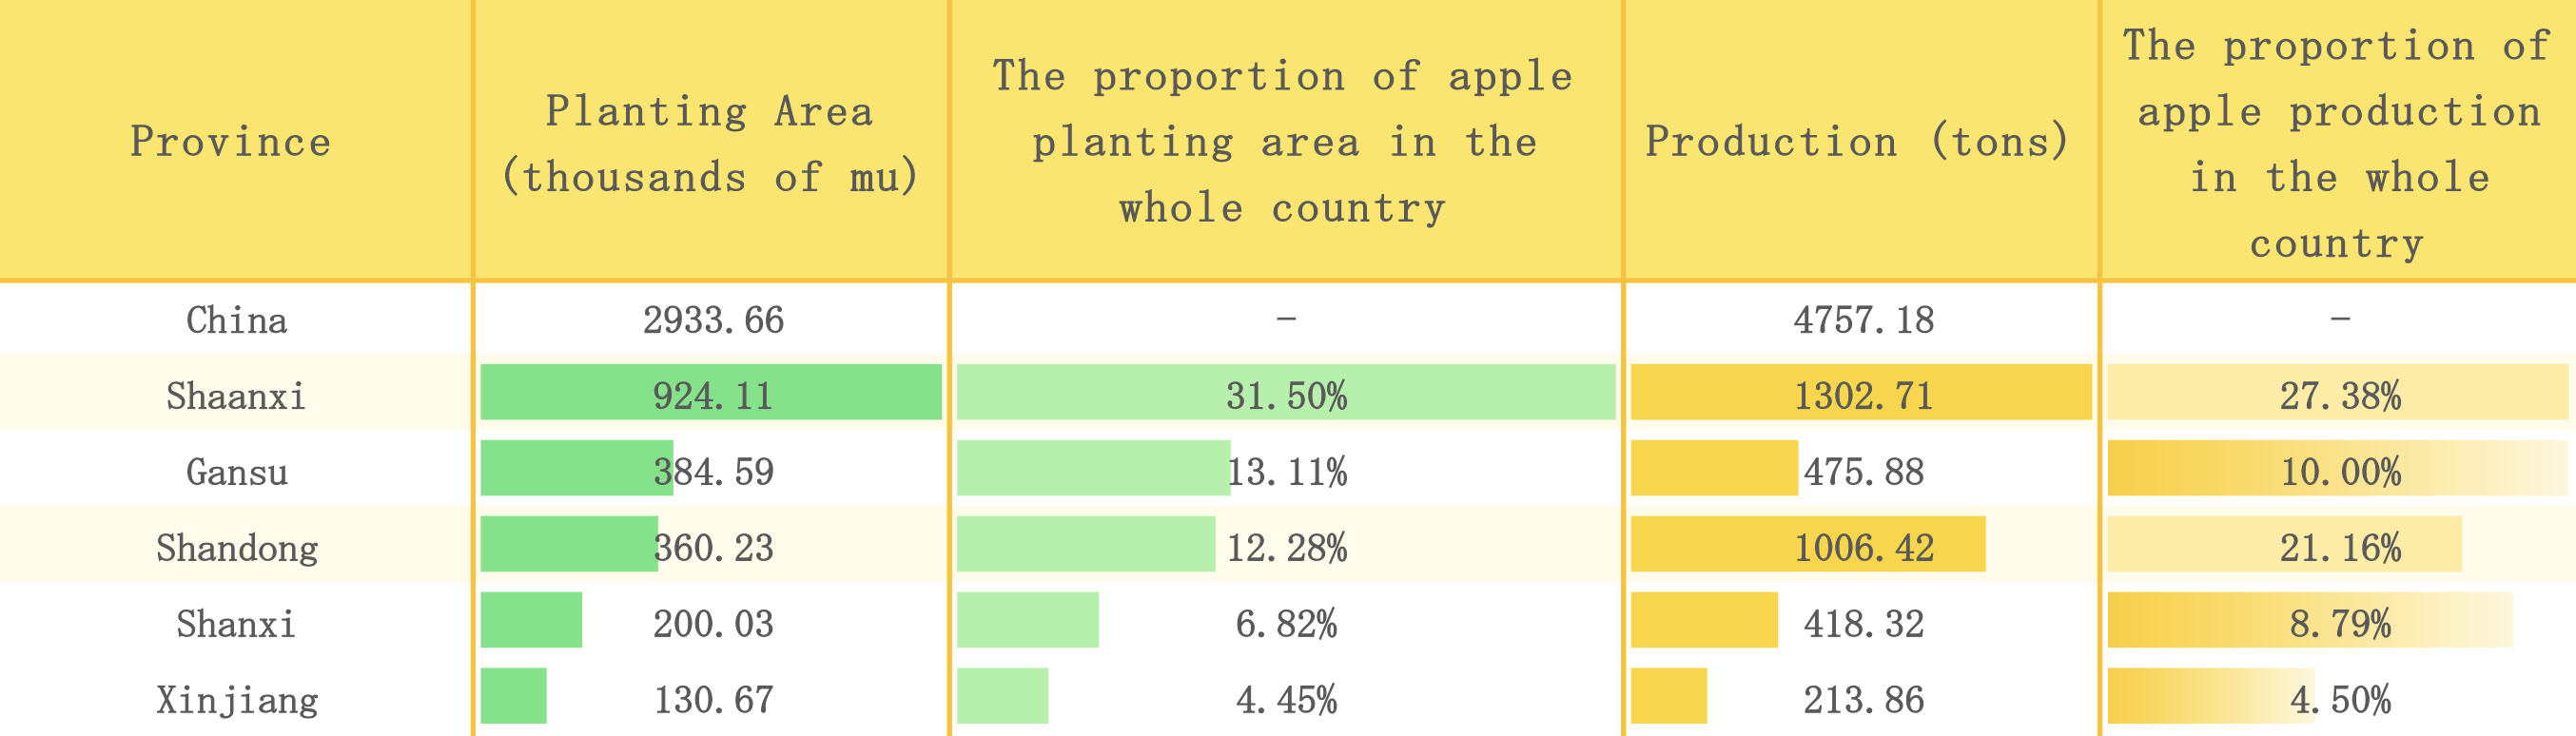
\includegraphics[width=\linewidth]{tables/production_provinces_table.png}
    \label{tab: production provinces}
    \begin{tablenotes}
    \footnotesize
    \item Note: The table reports absolute values (planting area in thousands of mu and production in tons) alongside each province's share of the national total. Embedded bar charts provide a visual comparison of relative magnitudes across provinces. Source: FAOSTAT and China National Bureau of Statistics
    \end{tablenotes}
\end{table}


While the national figures provide a broad overview of China's apple industry, the regional dynamics are equally important for understanding the intricacies of this market. As shown in Table~\ref{tab: production provinces}, one province stands out as a critical player in this context—Shaanxi. The phrase ``The world looks to China for apples, and China looks to Shaanxi'' captures Shaanxi Province's prominent role as the world's largest contiguous high-quality apple growing area. Shaanxi is one of China's leading apple-producing provinces, identified by the FAO as a core contributor to national output \citep{FAO2004}. Its apples have also gained international recognition through registration as a Protected Designation of Origin in Europe \citep{UKGov2021}. As the leading region for both apple cultivation area and production volume in China, Shaanxi produced 13.75 million tons of apples in 2023, accounting for around 28\% of the national total.

As a representative region in China's apple industry, Shaanxi faces significant challenges in the storage and distribution of its apples. As a storable fruit, apples have the potential to extend their market reach beyond the harvest season. But the province's storage capacity—estimated at around 5.8 million tons—is insufficient to meet the demands of local farmers and fruit traders. This shortfall points to an underdeveloped cold storage infrastructure, which affects not only the efficiency of the supply chain but also the income stability of the farmers. This gap in storage capacity is a crucial element to consider in understanding the market dynamics of Shaanxi's apple industry, and it serves as a backdrop for our later analysis of the broader market structure of the fresh apple supply chain.



\subsubsection{Import and Export Patterns}
\noindent Despite China's leading position in apple production, the country faces significant challenges in the global apple market, particularly with regard to export volume. While Chinese apples are widely consumed domestically, their export volume remains relatively small compared to domestic consumption. The primary reason for this is not necessarily issues with quality, but rather the lack of brand awareness of Chinese apples in international markets. 

Most fruit merchants in China have not focused on developing apple export opportunities, due to limited branding, international market penetration, and a lack of export channels, logistical support, and export-friendly policies. While Chinese apples meet quality standards, the industry's weak infrastructure for promotion and distribution has hindered growth in export markets. As shown in Figure \ref{fig: import export}, China's exports are more variable compared to the U.S., indicating challenges in retaining international customers.

\begin{figure}[hpt]
    \centering
        \caption{Import and Export Quantities for China and USA from 1961 to 2022}
    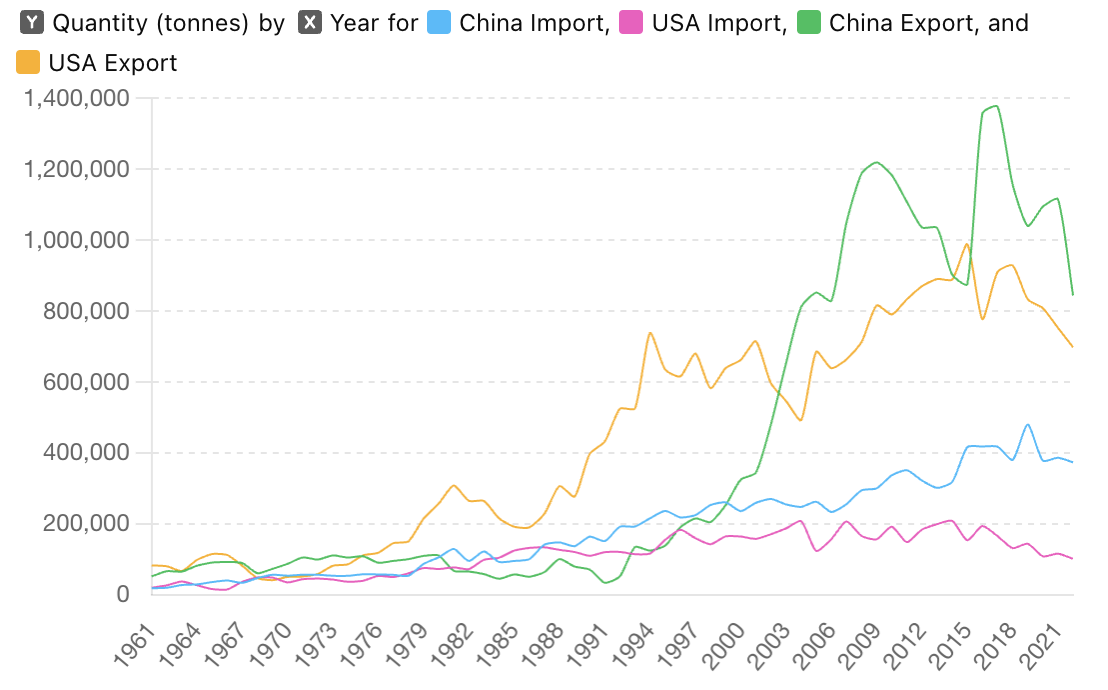
\includegraphics[width=\linewidth]{figures/import_export.png}
    \label{fig: import export}
    \text{Source: The Food and Agriculture Organization Statistical Database (FAOSTAT)}
\end{figure}

In 2023, China had a net export position in the apple trade, with exports reaching 1.07 million tons. Fresh apple exports are relatively diversified across trade partners, with key export destinations including Southeast Asian countries such as Vietnam, Indonesia, Thailand, and Bangladesh, which collectively account for over 75\% of total Chinese apple exports. Shandong province, located along the coast, contributes around 55\% of these exports. Although Shaanxi is another major apple-producing region, its inland location limits its export capacity, accounting for less than 3\% of the national total. Export activities typically peak from September to December each year.

On the other hand, as shown in Figure \ref{fig: import export}, China's imports have remained relatively flat, highlighting its strong domestic consumption and minimal reliance on foreign apples, of 98,200 tons in 2023.  Import volumes are concentrated during the latter half of the production cycle, from April to August, when domestic inventories are low. New Zealand is the leading source of apple imports, accounting for approximately 60\% of total imports. Among China's provinces, the coastal regions of Guangdong, Shanghai, and Zhejiang make up over 95\% of the total apple imports, and relatively rich urban residents mainly consume these imported apples.





    
\subsection{Supply Chain Dynamics}
\noindent China's fresh apple supply chain is characterized by a highly fragmented structure, seasonal supply-demand imbalances, and limited cold chain logistics, all of which restrict supply chain efficiency and contribute to significant price volatility, ultimately impacting the industry's development.

The apple-growing segment combines regional concentration with dispersed production patterns. Key regions like Shaanxi and Shandong provinces have some clusters of concentrated orchards. Still, a significant portion of apple cultivation is managed by small-scale farmers who rely on traditional practices. This uneven production and management structure often results in fluctuations in yield and apple quality, adding variability to the supply chain.

Inefficient storage presents a critical bottleneck in the midstream segment of the apple supply chain. This issue leads to an oversupply of apples during the harvest season, driving prices down, while limited off-season inventory exacerbates price volatility due to constrained supply. The midstream market is characterized by low horizontal integration, with small- and medium-sized buyers playing a pivotal role. These buyers typically purchase apples directly from farmers, conduct initial sorting and packaging, and then sell to wholesalers (aggregators) or retailers. 

Notably, demand from the food service sector, such as restaurants, is minimal compared to household consumption. While specific data on the share of fresh apple consumption attributed to the food service industry in China is scarce, insights from my 2024 interview with the China Apple Industry Association corroborate this observation.



\begin{figure}[hpt]
    \centering
        \caption{Supply Chain of Fresh Apple Industry}
    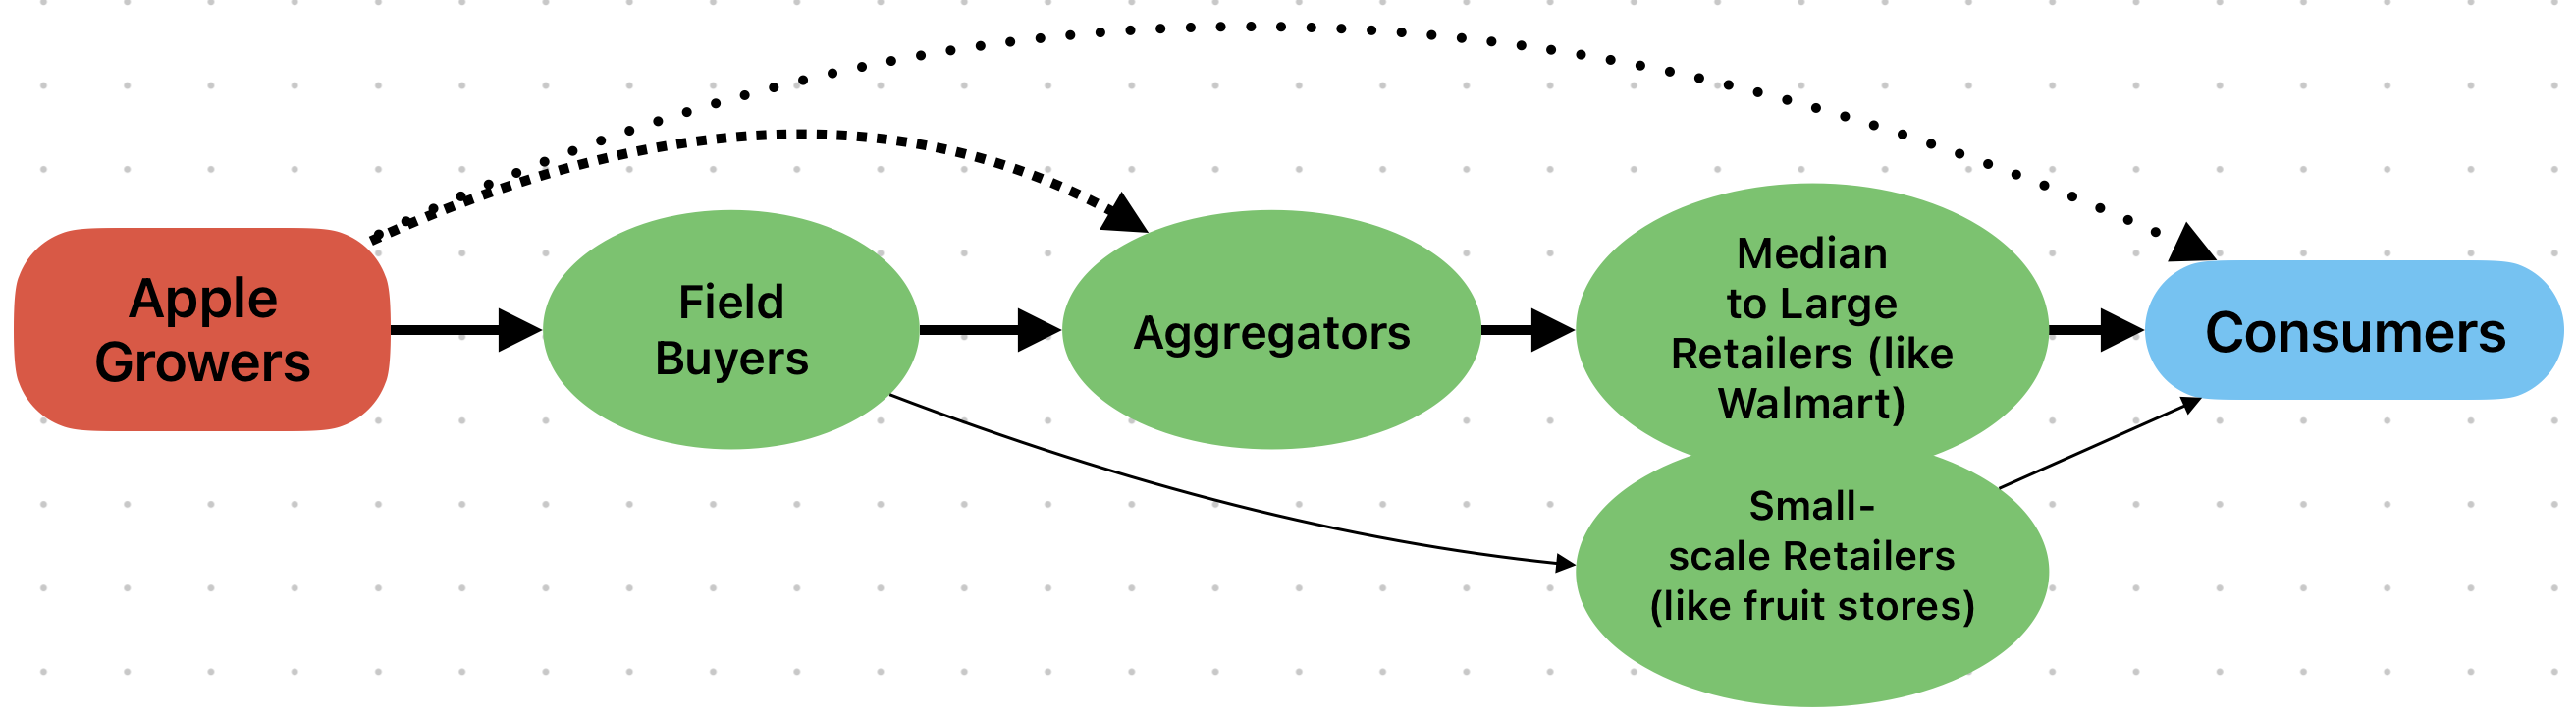
\includegraphics[width=\linewidth]{figures/Supply_Chain_flow.png}
    \label{fig: supply chain flow}
\end{figure}
The apple supply chain flows from growers to consumers through at most three layers of intermediaries, as shown in Figure \ref{fig: supply chain flow}. Each intermediary plays a distinct role, though each trader or firm may shift between roles based on timing, pricing, and market conditions. I categorize these intermediaries into kinds and define them as follows:

\begin{itemize}
    \item \textbf{Field Buyers}: These are small-scale traders who purchase apples directly from growers. Field Buyers act as the first point of aggregation, sourcing apples from orchards.
    
    \item \textbf{Aggregators/Wholesalers}: These intermediaries, often comprising larger wholesalers or processors, purchase apples from Field Buyers. Aggregators play a crucial role in consolidating apples from various sources and may add value through sorting, packaging, and broader distribution. Depending on the timing and market price, larger traders or wholesalers may also procure directly from growers, temporarily functioning as Field Buyers.
    
    \item \textbf{Retailers}: The final link in the supply chain, retailers acquire apples from Aggregators (or occasionally from Field Buyers) and sell them directly to consumers. Retailers range from major supermarkets, like Walmart and Carrefour, to smaller local stores, making apples accessible to the end consumers.
\end{itemize}

While these intermediary roles are generally stable, a trader or firm may switch between them based on circumstances---for example, a wholesaler may act as a Field Buyer during certain periods of the crop year if it offers a cost advantage. This adaptability allows the fresh apple supply chain to respond flexibly to changing market dynamics and crop cycles.




\subsubsection{Leaving the Orchard: Marketing Choices of Apple Growers}
\noindent This section addresses how apple growers sell their produce and make inter-temporal marketing decisions. First of all, the marketing timeline of primary growers is as follows: 

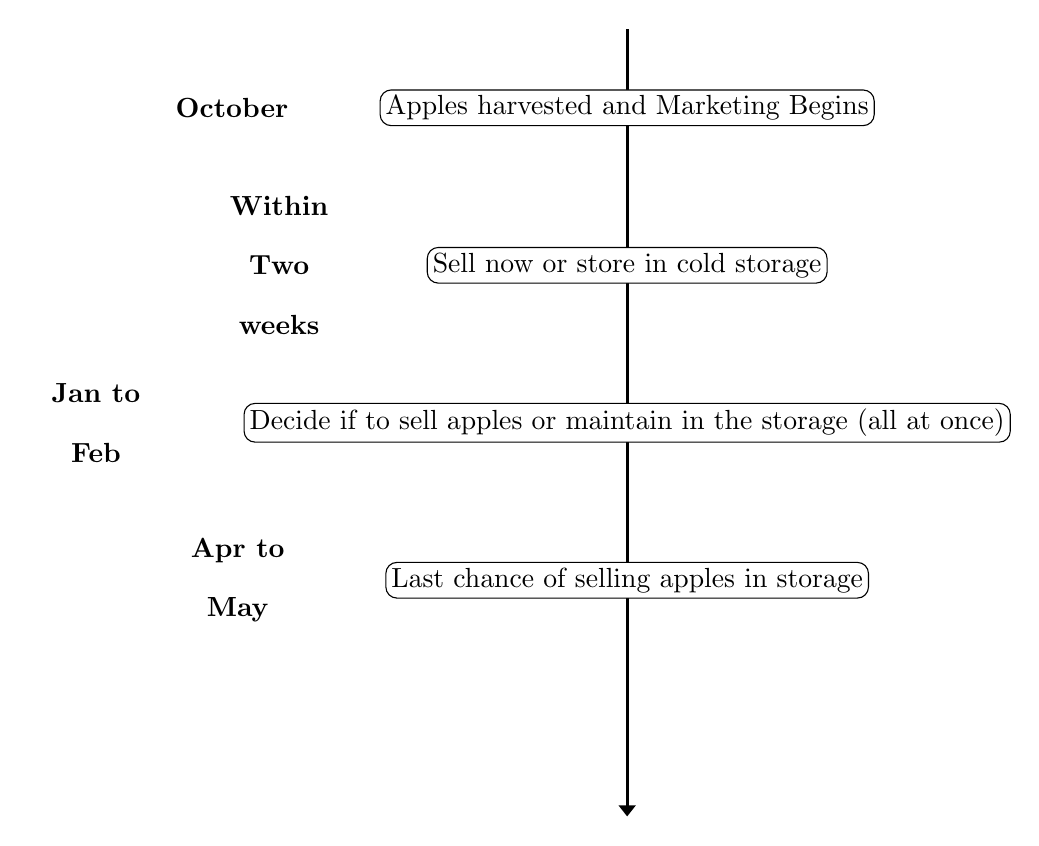
\begin{tikzpicture}[
  timeline/.style={line width=1pt, draw=black, -{Triangle[length=4pt, width=6pt]}},
  event/.style={draw, fill=white, rounded corners, inner sep=2pt},
  year/.style={text width=1.5cm, align=center, font=\bfseries}
  ]

  % Vertical Timeline (extended to handle more events)
  \draw[timeline] (0,0) -- (0,-10);

  % Events
  \node[event] (event1) at (0,-1) {Apples harvested and Marketing Begins};
  \node[event] (event2) at (0,-3) {Sell now or store in cold storage};
  \node[event] (event3) at (0,-5) {Decide if to sell apples or maintain in the storage (all at once)};
  \node[event] (event4) at (0,-7) {Last chance of selling apples in storage};

  % Years
  \node[year, left=of event1] {October};
  \node[year, left=of event2] {Within Two weeks};
  \node[year, left=of event3] {Jan to Feb};
  \node[year, left=of event4] {Apr to May};


\end{tikzpicture}


Farmers typically harvest their apples in mid to late October. Within two to three weeks of harvest, they face their first critical decision: whether to sell or to store the apples. Sales generally occur through two primary channels:

\begin{enumerate}
    \item \textbf{Direct Negotiation with Field Buyers}: The most common practice is to sell to small merchants who visit villages during harvest, inspect the apples on-site, and negotiate prices directly in the field.
    \item \textbf{Contract Sales to Large-scale Buyers or Aggregators}: Some farmers seek contracts with larger merchants, as these arrangements provide greater security and often include minimum procurement prices. Yet only a small fraction of farmers can secure such contracts, since large merchants purchase mainly high-quality produce from sizable suppliers. Farmers also express hesitation about dealing with smaller merchants, who are perceived as less reliable and more likely to renege on agreements.
\end{enumerate}

This initial trading period lasts roughly two weeks. If farmers are unable to sell or choose not to sell their apples during this time, they must store them in cold storage and wait for another opportunity to sell.

While farmers can sell their apples at any time once they are in cold storage, there are two main marketing windows:

\begin{itemize}
    \item \textbf{The First Window}: Around January and February, coinciding with the Chinese Spring Festival. If farmers believe this is the highest price they can get, they will sell their apples at this time.
    \item \textbf{The Second Window}: If they hold onto their apples longer, the next opportunity to sell usually arises between late March and early May, around Labor Day.
\end{itemize}

Traditionally, apple growers sell their entire harvest at once when they encounter favorable pricing rather than gradually selling over time, even if prices fluctuate. This behavior is shaped by market dynamics and a preference for one-time cash inflow.

Two primary marketing channels discussed above dominate the initial stage of apple trade in China, but a small number of growers are beginning to explore direct-to-consumer sales through innovative methods. Leveraging platforms like WeChat and TikTok, these farmers are adopting multi-period smoothing sales strategies. While e-commerce currently represents only a negligible share of total sales, it offers significant advantages. This approach not only reduces information asymmetry but also allows farmers to gain a more comprehensive understanding of the supply chain, enabling them to make more informed and efficient decisions.


Moreover, most apple growers in China do not have fixed trading partners. While they may be familiar with some traders, these relationships lack strong binding ties. Farmers in the fieldwork site exhibited a strong preference for large-scale traders. These giant merchants offer greater stability and credibility, as they are perceived to have lower market failure rates compared to smaller traders. When farm-gate price differences are marginal—typically within 0.2 RMB/kg—farmers tend to favor large traders, prioritizing reliability and security over minor price advantages.




\subsubsection{Connecting the Ends: Distributing Channels of Intermediaries}
\noindent As shown in Figure \ref{fig: supply chain flow}, field buyers play a critical role in the apple supply chain, distributing apples either to aggregators or directly to small fruit shops. They operate using three main strategies, which are representative of their diverse roles:

\begin{enumerate}
    \item \textbf{``Immediate in-and-out Buyers''} These buyers operate on demand-driven purchases from downstream agents. They procure apples directly from farmers and immediately transport them to downstream agents without any storage, aligning their operations with real-time demand.

    \item \textbf{``Arbitrage Sellers''} Similar to aggregators, these buyers focus on leveraging inter-temporal price differences. They typically make a single bulk purchase, store the apples in cold storage (either their own or that of larger traders), and sell them later when prices are higher.

    \item \textbf{``Cooperative Agents''} These buyers are also apple growers who leverage their strong local social networks and access to village-level information. They typically purchase smaller quantities from local farmers and resell them to large-scale traders, acting as intermediaries.
\end{enumerate}

Aggregators, on the other hand, often establish long-term contracts with large-scale retailers such as Walmart and Carrefour, ensuring stable supply relationships. For example, in Yanchang County, the largest aggregator, \textit{China Agricultural Products Group Ltd (Yanchang branch)}, is a key supplier of fresh apples to \textit{WUMART Stores, Inc.}, which operates over 100 grocery stores in Beijing. Despite their direct procurement efforts during the peak trading season, the fragmented nature of apple production in China forces aggregators to rely heavily on field buyers for their supply.

Meanwhile, small- to medium-sized retailers, such as street-side fruit shops in urban areas, often bypass aggregators and source directly from field buyers. This approach allows them to secure lower procurement costs or obtain unique, high-quality apples that distinguish their offerings from those of large-scale retailers, thereby carving out their own market niche.

While international demand accounts for only a small portion of the total fresh apple consumption in China, exporters often maintain greater vertical integration compared to purely domestic players. Companies like \textit{Yantai North Andre Juice Co.} and \textit{Shaanxi Fruit Industry Group Co.} employ dedicated procurement teams to ensure their apples meet international quality standards. These teams establish long-term relationships with farmers, offering technical and financial support to achieve product consistency.

China's apple exports are primarily destined for Southeast Asian countries, where consumers often prefer smaller-sized apples rather than the widely cultivated Red Fuji variety. To meet this demand, exporters must develop their own supply sources instead of relying on existing orchards and intermediaries.




\subsubsection{Middlemen Scale and Supply Chain Roles}
\noindent The scale of a buyer is closely tied to its role in the supply chain. Smaller buyers typically have less capital, lower purchasing volumes, limited storage capacity, and reduced risk tolerance. However, their trading strategies tend to be more flexible. As a result, small buyers rarely sign long-term supply contracts with downstream clients. During the initial trading period following the harvest, they often wait for large buyers to set the market price before making their moves.

Intuitively, one might question why small buyers persist on a large scale if they seem to lag behind large buyers in every aspect. The key lies in their role as field buyers within the supply chain. Their greatest value is their ability to reach fragmented and scattered micro-scale apple producers in a way that is not as visible or accessible to larger buyers. This effectively extends the supply chain extensively. At the same time, small buyers often exploit the information asymmetry inherent in these small-scale trading relationships to generate excess margins.

In my fieldwork region, Yanchang County, there are four large-scale fresh apple traders, primarily serving as aggregators. With large cold storage facilities (over 5,000 tons), these traders purchase fresh apples from farmers exclusively during the initial trading period after the harvest (mid-to-late October), fulfilling their annual procurement needs in one go. In contrast, hundreds of small-scale buyers emerge in the county each year, sourcing apples from farmers over a dispersed period of six to eight months after the harvest.

For apple farmers, becoming a supplier to large-scale traders is challenging due to their stringent requirements, which often include larger orchard sizes, higher fruit quality, and a proven track record of honoring contracts. Unfortunately, given the constraints of production conditions and education levels in developing regions like northern Shaanxi, China, most farmers in these areas are left with no choice but to sell their apples to small-scale buyers.

From the perspective of end consumers, demand is diverse and virtually limitless. Thus, small-scale retailers can always find niches, which have not been satisfied by supermarkets, to thrive in—whether through geographical market segmentation, offering a variety of apple qualities, or aligning with niche brands.

In summary, in the fresh apple industry in China, small-scale buyers typically occupy the two ends of the intermediary spectrum illustrated in Figure \ref{fig: supply chain flow}: they exist as field buyers and small-scale retailers. Their foundation lies in the diverse and dispersed nature of suppliers and consumers.




\subsubsection{Dynamics of Local and non-local Traders \label{Section: intro of Local and non-local traders}}
\noindent Similar to many other agricultural commodity markets, such as California's tomato industry \citep{hamilton2024spatial}, China's fresh-apple procurement markets are often localized at the county level. These markets are characterized by a limited number of buyers and the potential for hold-up due to costly cross-county transportation and the perishability of apples. Consequently, most intermediaries fall into two distinct groups: ``local traders'' and ``non-local traders.''  

``Local traders'' refer to merchants based in the same county, whose primary trading activities are also concentrated within the county. In contrast, ``non-local traders'' are merchants from other regions who specifically travel to the county to purchase apples.  

Local fruit traders are mostly small-scale operations. They typically earn a margin by reselling to non-local traders rather than directly supplying downstream markets themselves. According to a local trader in Yanchang County, Wenkui Liu, \say{only a small fraction of them handle downstream distribution on their own. In contrast, non-local traders who come to purchase fruit are usually more established and often have their own dedicated apple distribution channels.}

Local traders typically have a deeper understanding of local apple production, knowing exactly which villages or even households consistently supply high-quality and reliable products. They are also well-acquainted with the distribution of cold storage facilities, government regulations, and other county-specific information critical to the apple supply chain upstream. Therefore, in economically developed regions with high-quality apple production, local traders are often numerous and dominant, unwilling to relinquish their control over the upstream supply chain to outsiders. non-local traders entering these regions must compete with local traders at an intrinsic disadvantage. Therefore, most non-local traders resort to ``subcontracting'' local traders to source apples on their behalf, forfeiting part of their profit margins.  

Conversely, in economically less developed areas, non-local traders tend to have a higher market share. This is partly because local traders with a solid understanding of the market often migrate to high-quality production areas in search of better opportunities. Additionally, non-local traders frequently serve more diverse purchasing needs, such as supplying lower-quality apples to juice factories or taking advantage of weaker relational considerations and negotiation costs in less developed areas, where bargaining power may be more favorable to buyers.  

Moreover, some traders purchase apples from lower-quality production areas and then repackage or store them in high-quality regions, thereby disguising their origin to command higher prices. For instance, apples from Yantai in Shandong Province have established a strong reputation nationwide. In recent years, however, many ``non-local'' apples have been stored in Yantai's cold storage facilities, only to be sold later under the Yantai label at premium prices. Downstream buyers often find it difficult to distinguish these apples from the genuine local produce, leading to significant brand and regional price markups to those non-local traders.


\subsection{Roles of Storage \label{Section: role of Storage}}
\noindent In China's fresh apple industry, storage serves multiple roles across different stages in the fresh apple supply chain, stabilizing inter-temporal supply, maintaining apple quality, and managing market dynamics across seasons. As a storable agricultural product, the shelf life of apples can be significantly extended by using cold storage. Apples can be preserved for several months, or even up to a year, in a cold storage environment at 0°C-1°C and 85\%-90\% humidity, whereas at room temperature, they can only last for a few weeks.

The use of cold storage facilities is highly diversified and fragmented, with the entire supply chain relying on cold storage, and the distribution ratio changing each year. From the perspective of market efficiency theory, most apples awaiting sale should ideally be stored in cold storage with the lowest unit cost, which is typically in the ultra-large cold storage facilities owned by major fruit traders. However, due to various transaction frictions and information asymmetry, large traders' cold storage facilities tend to hold a complex inventory, with around 50\% of the stock on average consisting of apples owned by the storage owners themselves. The remaining stock is mainly stored on behalf of various small traders and local, experienced apple growers.

At the farm level, after picking, farmers make initial decisions about selling vs. storing. Storage enables them to delay sales until market conditions improve, allowing them to wait for higher prices in off-peak seasons, which can improve their overall income level. Additionally, storage facilities provide smallholders with the flexibility to sort and grade apples at their own pace, reducing post-harvest losses and maintaining quality. However, their storage options are limited and often depend on available infrastructure nearby. Despite a few forward-thinking farmers building their own small cold storage facilities, the overall adoption rate of cold storage among apple growers remains low. With government subsidies, many villages have built medium-sized cold storage facilities with capacities of several hundred tons, collectively owned. However, this leads to a low individual harvest-to-storage-volume (HSV) ratio, mainly because of the high storage cost. This is because the use of such collectively-owned cold storage requires multiple farmers to coordinate their decisions after harvest, which often is very hard.

Intermediaries purchase apples from farmers, either for immediate resale or for storage. For them, storage serves as a key function for aggregating apples from different growers. This aggregation enables sorting, grading, and packing before the apples move to larger markets or processors. It also provides intermediaries with greater bargaining power by controlling the flow of apples into the market, allowing them to release apples gradually and manage supply to influence prices. This is particularly important in an oligopsonistic market structure, where a small number of buyers dominate the market. Furthermore, storage ensures quality assurance for downstream buyers, such as wholesalers and retailers, by maintaining apples in optimal conditions, ensuring they meet high-quality standards, especially for urban markets or export.

Retailers, especially in urban areas, rarely own or rent storage facilities specifically for fresh apples but usually cooperate with large-scale intermediaries, signing long-term supply contracts and leaving apples in the suppliers' facilities. Once there is a potential shortage of apples on the shelves, apples can be replenished from the supplier's cold storage at any time. This practice supports retailers' stock management, helping retailers avoid overstocking while still ensuring that apples are available to customers.

Finally, for apples intended for export, storage is essential for maintaining quality during transit. Export-ready apples, especially those shipped long distances to markets in Southeast Asia and other regions, often require controlled atmosphere storage to preserve freshness, appearance, and taste. This storage minimizes spoilage risks during shipping and helps meet the stringent quality requirements of international markets.




\subsubsection{Storage Pricing Structure: Based on Quantity, Not Duration} 
\noindent Cold storage fees for fresh apples are typically based on quantity rather than duration, which may seem counter-intuitive. This pricing structure stems from the fact that apple harvesting occurs within a narrow window (mid-October to mid-November), creating a surge in storage demand during that period. Additionally, apples can only be stored for up to a year, requiring them to be sold two or three months before the next harvest. This arrangement provides cold-storage users with a longer marketing window without any additional cost, reducing the pressure to accept lower prices from downstream buyers and giving them more flexibility in timing their sales.

\subsubsection{Shortage and Inefficient Allocation in Cold Storage Infrastructure} 
\noindent In 2022, China's total apple storage capacity exceeded 20 million tons, with mechanical cold storage accounting for approximately 70\%, simpler storage methods making up around 25\%, and high-end controlled atmosphere storage comprising about 5\%. Over the past decade, advancements in technologies such as intelligent sorting, rapid pre-cooling, 1-MCP (1-methylcyclopropene) treatment, 0°C-1°C storage, and specialized preservation bags have significantly improved the commercial quality of apples and substantially reduced post-harvest loss rates.

However, given the large scale of domestic apple production and the fact that many production areas are situated in underdeveloped and poorer regions, there is a notable shortage and inefficient allocation of cold storage infrastructure. In more economically developed provinces and counties, such as Shandong, there are more cold storage facilities with larger capacities. For instance, in 2022, Shandong's total cold storage capacity was around 5.4 million tons, with actual storage usage remaining stable at approximately 4.8 million tons in recent years. The ratio of apples stored by farmers compared to those stored by traders is approximately 70\% to 30\%. On the other hand, in remote regions like northern Shaanxi and Xinjiang, the situation is starkly different: cold storage facilities are limited, and the storage needs of farmers and small-scale traders cannot be fully met. As a result, the proportion of apples in storage fluctuates significantly each year, driven largely by market conditions and sentiment.

At the micro-level, in my fieldwork area, Yanchang County, the prevalence of small, self-built cold storage units among farmers is less than 5\%. Most apple growers are forced to sell their apples immediately upon harvest or rent cold storage space from facility owners, typically traders. The cold storage capacity in this county is fully utilized each year, meaning that overall storage capacity falls short of the demand.
    







\subsection{Apple Futures Market: The World's Only Fresh-Fruit futures}
\noindent Launched on the Zhengzhou Commodity Exchange (ZCE) in 2017, China's fresh apple futures market is the world's only futures market dedicated to fresh fruits. As China leads global apple production, accounting for over half of the world's supply, this market was designed to address the apple industry's high price volatility and provide much-needed price risk management tools for farmers, traders, and buyers.

Uniquely focused on fresh rather than processed apples, this futures market stands out from traditional agricultural futures, which typically center on commodities that are shelf-stable and have relatively low storage requirements. The contract is based on the widely consumed Red Fuji variety. Contracts require high-quality apples that meet rigorous standards for both domestic and export markets, ensuring that delivered products align with consumer expectations.

The apple futures market serves as a vital bridge between various industry players, including growers, traders, processors, and exporters. By establishing a transparent pricing mechanism, it helps participants manage price risks effectively, especially in a market where prices can vary widely due to seasonal cycles, regional production differences, and changing demand. For example, in years with poor harvests, prices can rise as much as 20\%, while bumper years can see sharp price drops. Futures contracts allow growers and traders to lock in prices in advance, protecting against such fluctuations.

However, the perishable nature of apples poses logistical challenges. Maintaining quality during storage is critical for contract fulfillment, as fluctuations in storage conditions can affect both quality and price. Most apple futures contracts are executed from October through February to align with peak harvest periods, ensuring optimal product quality and reducing the need for long-term storage. 

Participation in the futures market, though, remains challenging for smaller farmers. Limited access to capital and a lack of trading knowledge can hinder direct engagement. 


%----------------------------------------------------------------%
%----------------------------------------------------------------%

\newpage
\section{Upstream Buyer Power, Market Structure, and Competition \label{Section: market structure}}
\noindent 
Research in the industrial organization (IO) of agricultural markets—both in developing and developed economies—has traditionally focused on the exercise of monopoly power in the sale of farm inputs, processed foods, and food retailing \citep{macdonald2024introduction}. However, significant attention has also been directed toward understanding monopsony and oligopsony power in agricultural markets, where buyers wield considerable influence over pricing and farmers' production and post-harvest decisions \citep{kopp2021farmers, zavala2022unfair}.

The structure of China's fresh apple supply chain provides a particularly compelling case for exploring these dynamics. The combination of the industry's distinctive characteristics and its critical role in rural development makes it a fertile ground for bridging insights from development economics and industrial organization research \citep{bellemare2022agricultural}. China's fresh apple industry, which accounts for over half of global production, is renowned for its impact on poverty alleviation in some of the country's least-developed regions. The distributional impacts of market power exerted by intermediaries often outweigh its efficiency effects \citep{sexton2013market}.

This leads to a central question: Who really profits from China's apples?

\begin{quote}
    In 2020, an informal investigation by China's Ministry of Agriculture traced the journey of apples from orchards in Shaanxi to retail shelves in Shanghai—a 3,400-kilometer journey that saw prices increase more than fivefold. Initially, a field buyer purchased 3 kilograms of apples directly from farmers for 10 RMB. After transportation to Jiaxing and accounting for logistics costs, 10 RMB bought only 2 kilograms. Following additional sorting and distribution through wholesale markets, the same amount fetched just 1 kilogram. Finally, in Shanghai supermarkets, 10 RMB was exchanged for a mere 0.5 kilograms.
\end{quote}

This example underscores critical questions about the distribution of value along the supply chain and the competitive forces, or lack thereof, that shape outcomes for stakeholders.

Based on my fieldwork in 2023 and 2024, the apple market in Northwest China operates as a buyer's market. Apple farmers (sellers) function in a near-competitive market, while intermediaries (buyers) often exhibit collusion or even oligopsonistic behavior. While some argue that farmers could secure better prices through cooperatives, most local cooperatives are too small in scale compared to buyers' procurement volumes and face significant competition among themselves. Additionally, cooperatives are loosely organized, leaving most farmers to sell individually. Buyer competition, however, is closely tied to downstream demand. During periods of low demand, field buyers rarely compete, but in times of strong demand, intensified competition for market share drives up farm-gate prices.

This section examines the market structure and competitive dynamics in the upstream segment of China's fresh apple supply chain, with particular attention to buyer power. It addresses three core questions: (i) does collusion among buyers exist, and in what forms; (ii) why do competitive conditions among buyers vary across periods; and (iii) what role does storage play in mitigating buyer power. The analysis builds on descriptive micro-level evidence collected during fieldwork in Yanchang County, Shaanxi Province.

\subsection{Buyer Collusion}
\subsubsection{Collusive Behavior and Competition Among Local Traders}
\noindent 
Field evidence from Yanchang County suggests that local buyers may engage in forms of coordinated behavior that resemble cartel-like arrangements. At the county level, multiple such groups appear to operate simultaneously, though their presence becomes more limited at finer geographic scales—typically one to three groups within a town or village. These patterns can create market environments ranging from monopsony to oligopsony.

Within these groups, buyers often coordinate procurement activities and discuss strategies before purchasing apples. Communication channels such as WeChat groups facilitate information exchange on farm-gate prices and may help sustain discipline in pricing practices. Some buyers also described efforts to plan purchasing tactics collectively, which could shape local market outcomes. For example, one trader characterized these practices in the following way:

\begin{quote}
\say{My associates and I prearrange strategies to manage farmers' price expectations. On the first day, I might visit a village and offer a certain price without closing any deals. The next day, my colleague followed up with a deliberately lower price. Concerned about losing a buyer, farmers often agree to sell. This enables us to acquire apples at reduced prices.}
\end{quote}

The high degree of coordination among members within a cartel-like group reflects their strategic alignment in establishing an oligopsonistic bargaining position. According to another Buyer B:

\begin{quote}
\say{We avoid competition during the sourcing stage because our downstream distribution channels are almost entirely distinct from one another.}
\end{quote}

Despite the internal cohesion of individual groups, inter-group competition is presented. This inter-group rivalry is primarily driven by concerns over sourcing higher-quality apples and safeguarding supply sources. Yinfang Lei, the manager of \textit{Shaanxi ZhongGuo Ltd.}, a local aggregator, remarked:

\begin{quote}
\say{The competition between field-buyer cartels is intense. They are wary of other cartels capturing higher-quality apples or encroaching on their supply bases, which could undermine their market position. Consequently, cartels are generally unwilling to collaborate with one another.}
\end{quote}

The behavior of these cartel-like groups highlights classic dynamics in the field of industrial organization, where coordination within a group aims to enhance buyer power, while inter-group competition undermines broader collusion. The duality of cooperative and competitive forces underscores the complex strategic interactions within localized agricultural markets.



\subsubsection{Market Territories of Buyers}
\noindent The existence of market territories among buyers in Yanchang County is a subject of debate.

Although field-buyer cartels generally do not cooperate, traders within a given cartel coordinate their procurement areas, establishing informal market territories to avoid internal conflicts. For instance, Buyer A in LeiJiaTan Town noted: 

\begin{quote}
\say{A market territory does exist. I will not step into a village if another member of my group has already contacted it during the same crop year. This happens in about two-thirds of cases now.}
\end{quote}

As illustrated in Figure \ref{fig: Market Territory}, within Cartel 1, four traders procure apples separately from Villages 1, 3, 4, and 5 without interfering with each other. These market territories are not formally delineated but are instead based on verbal agreements. Each cartel redefines its internal market territories annually, ensuring flexibility to adapt to shifting procurement conditions. This yearly restructuring allows cartels to exert short-term buyer power, where future considerations are relatively less significant \citep{sexton2013market}. Enforcement of these informal agreements relies on implicit relational costs rather than explicit penalties, where the cost of defection is the potential loss of trust and cooperation within the group.

\begin{figure}[hpt]
    \centering
        \caption{Market Territory Allocation Among and Within Cartels in Yanchang County}
    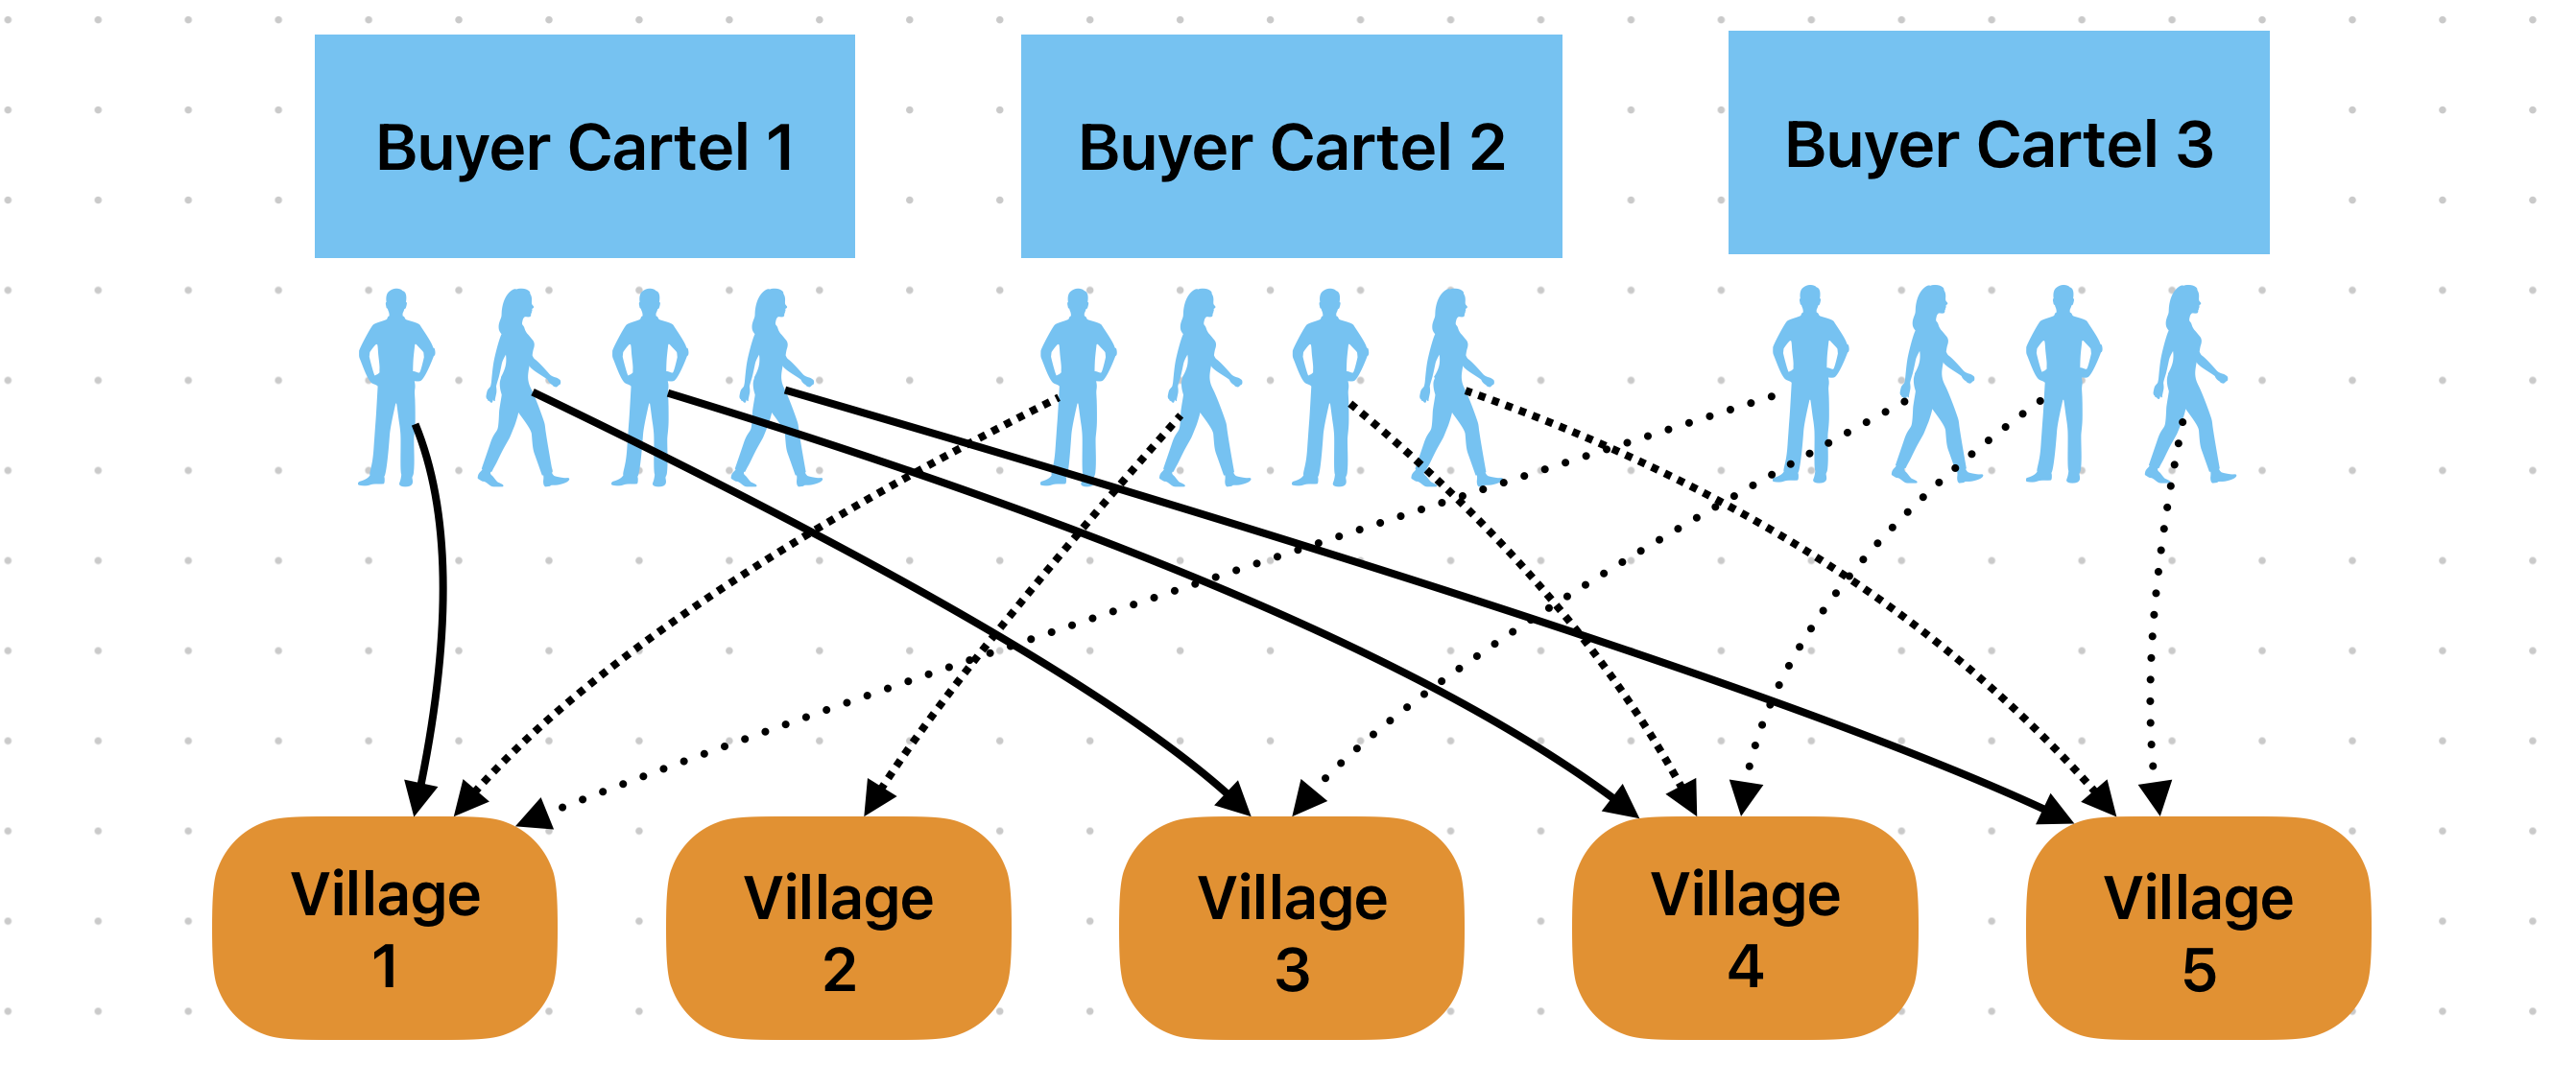
\includegraphics[width=\linewidth]{figures/Market_Territory.png}
    \label{fig: Market Territory}
\end{figure}

In contrast, there are no clear boundaries between the territories of competing cartels. Overlaps in procurement areas frequently arise, especially when multiple cartels target the same high-yield, high-quality orchards. As shown in Figure \ref{fig: Market Territory}, while Cartel 1 members respect internal market boundaries, Villages 1, 4, and 5—which produce superior-quality apples in large quantities—attract traders from all three cartels, creating an effective oligopsony. Conversely, in Village 2, only traders from Cartel 2, which is geographically closest, procure apples, resulting in a localized monopsony.

This overlapping of procurement territories among cartels demonstrates a dual dynamic: internal coordination fosters oligopsonistic market power within cartels, while external competition between cartels introduces inter-group rivalry, reducing market concentration. 



\subsubsection{Competition Between Local and Outside Traders}
\noindent 
As introduced in Section \ref{Section: intro of Local and non-local traders}, two types of apple traders operate in each county: local traders and non-local traders from outside areas.

In Yanchang County, most local traders do not manage downstream distribution themselves. Instead, they typically act as primary intermediaries (\textit{Daiban}), earning a margin by reselling apples to non-local traders or local aggregators as subcontractors. They can be categorized into:
\begin{itemize}
    \item Full Agents: Handle sourcing, sorting, and transportation, earning approximately 0.70 RMB/kg.
    \item Assistant Agents: Focus solely on matchmaking, earning about 0.08 RMB/kg.
\end{itemize}

Although local and non-local traders occasionally collaborate, as previously discussed, competition between them is more prominent. This competition arises because, for many non-local traders sourcing apples in Yanchang County, the additional costs associated with involving an additional local middleman often outweigh the benefits. As a result, non-local traders frequently bypass local traders by directly hiring local ``information agents'' to scout villages, inspect produce, and identify suitable suppliers. In many cases, non-local traders procure apples directly from farmers.

Interestingly, during the initial trading period, non-local traders often form one or more cartels to counteract local traders as well. According to a contact in Huasheng Fruit Co., a large fresh-apple exporter, \say{we, as non-local traders, commonly stay in the same hotel in the county's downtown area before heading to the villages for procurement.} These informal gatherings allow them to establish connections and organize interest groups, strengthening their collective bargaining position against local traders.






%----------------------------------------------------------------%

\subsection{The Paradox of Plenty: When More Buyers Deepen Farmer Challenges}
\noindent Is the degree of industry concentration always positively correlated with the extent of market power and negatively associated with the industry's output level and social welfare? An tuitive belief is that ``lots of buyers, must be competitive.'' However, \cite{kopp2021farmers} made the point that lots of buyers means nothing if they collude. More previous studies, such as \cite{merel2017buyer} and \cite{crespi2012competition}, challenge this conventional wisdom as well, demonstrating that the relationship may not always hold.

The upstream dynamics of China's fresh apple industry show that simply increasing the number of small-scale buyers does not necessarily improve market competitiveness or farmers' welfare. On the contrary, it can strengthen the dominance of large buyers by creating new layers of intermediation and reinforcing territorial segmentation, which further weakens farmers' bargaining position. By contrast, wholesalers and large traders may serve a pro-competitive role \citep{Belton_et_al_2024}. From a regulatory perspective, fewer but larger buyers may actually be preferable: they are easier for governments to monitor, more amenable to antitrust oversight, and more accountable for their pricing practices.


\subsubsection{``More but Dispersed'' or ``Less but Regulated''?}
\noindent While it is a common belief among development economists that more traders in a market imply higher competitiveness, this assumption may fail in agricultural procurement markets. For instance, in scenarios where an oligopsony exists, when several large-scale dominant buyers exercise significant control, small-scale traders typically function as intermediaries rather than as true competitors. Instead of challenging the incumbent buyers' market power directly, these small-scale buyers might act as middlemen, purchasing from farmers to resell to the dominant buyers. 

In fact, a tacit agreement might even exist between the dominant large-scale buyers and these small-scale traders. Rather than acting as independent competitors, these small-scale buyers can be seen as informal extensions of the incumbents' operation, effectively functioning as outside employees or contractors. This arrangement allows the dominant buyer to maintain control over the supply chain indirectly, leveraging the small-scale traders to handle transactions with suppliers while still dictating terms and prices. Consequently, the presence of multiple traders does not necessarily dilute the incumbent buyers' influence; it may even reinforce it, thereby sustaining or worsening the oligopsonistic structure and limiting fair pricing for farmers.

\begin{figure}[ht!]
    \centering
        \caption{Comparison of Buyer Structures: ``More but Dispersed'' vs. ``Less but Regulated''}
    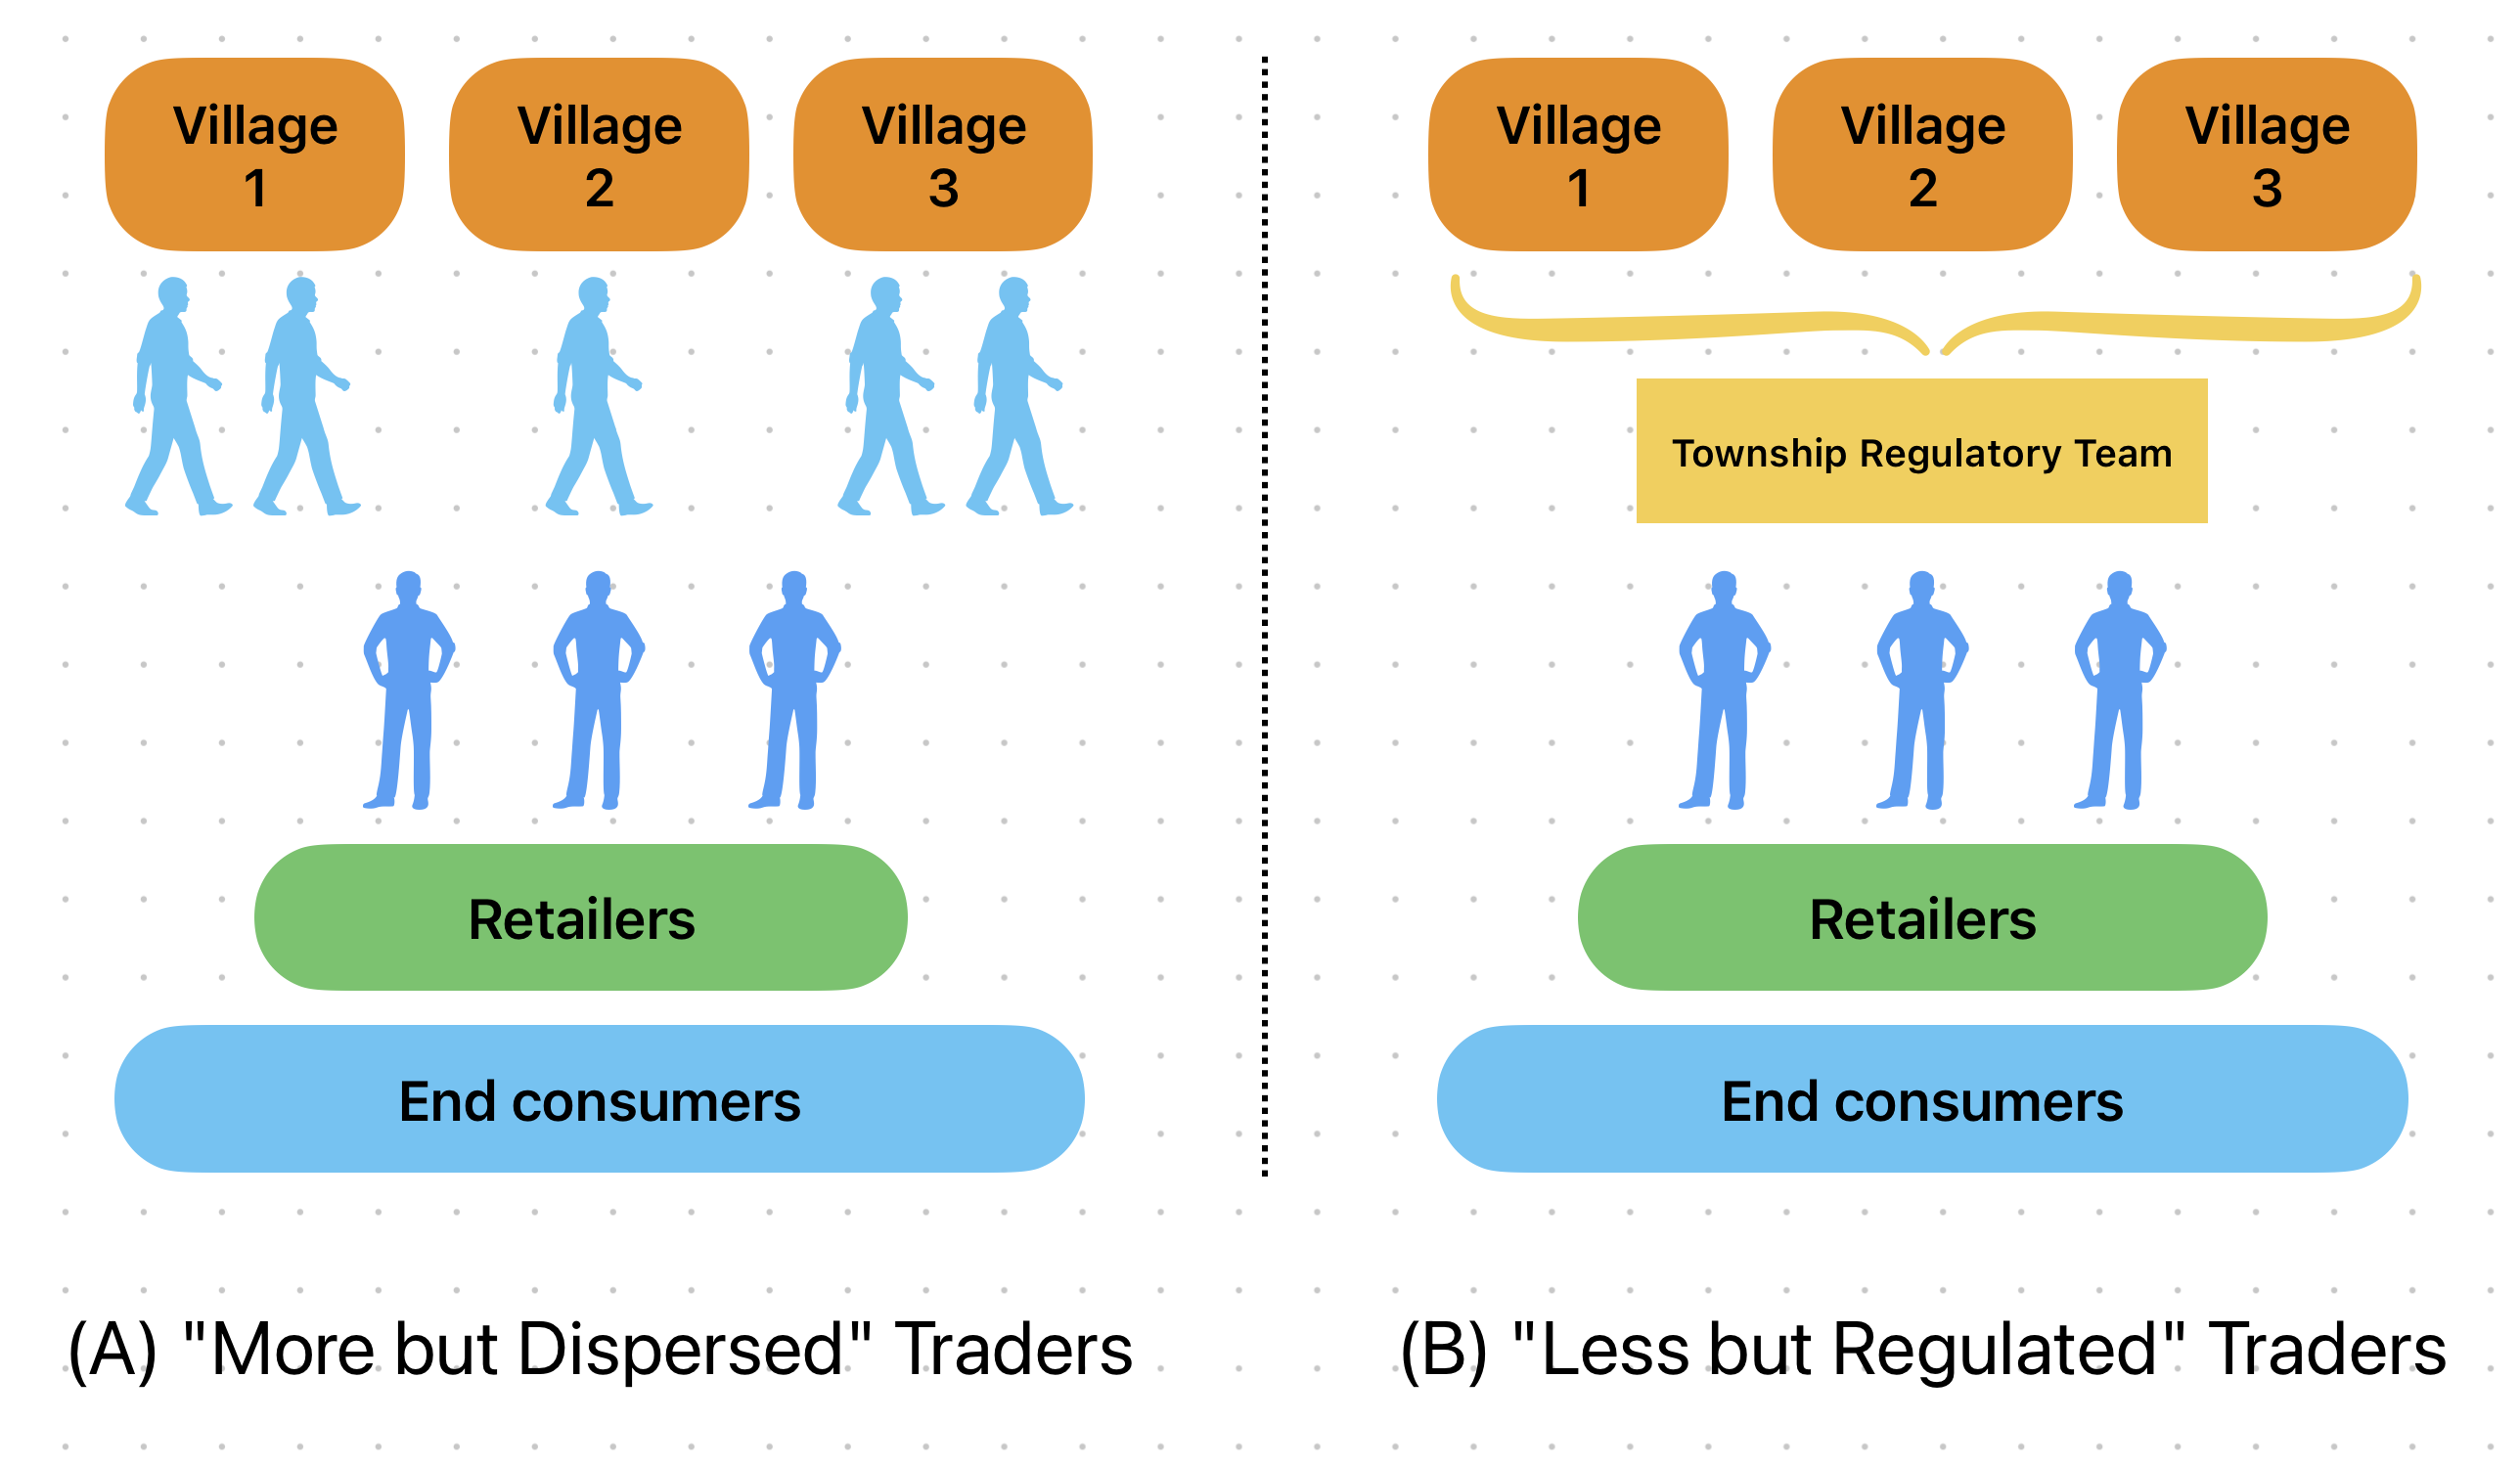
\includegraphics[width=\linewidth]{figures/more_is_less.png}
    \label{fig: more is less}
    \begin{tablenotes}
    \footnotesize
    \item Note: Light blue figures denote small-scale traders, while dark blue figures denote large-scale traders. 
    \end{tablenotes}
\end{figure}

In other words, as illustrated in the left panel of Figure \ref{fig: more is less}, these small-scale buyers may add another layer of intermediation, instead of competing with the incumbent buyers. Beyond these vertical impacts on the industry structure, an increase in entrant buyers also introduces horizontal market segmentation, often along geographic lines, which could possibly further lead to lower farm-gate prices, higher consumer prices, and significant price fluctuations across regions and over time, resulting in substantial welfare losses \citep{bergquist_McIntosh_2024}.


My fieldwork conducted during the 2023 and 2024 harvest seasons in Yanchang County revealed that over a hundred buyers traveled to various towns to procure apples each year. These buyers formed several field-buyer cartels, characterized by implicit arrangements on market territory allocation, as discussed in Figure \ref{fig: Market Territory}. As a result, farmers in each village were compelled to negotiate with a limited number of designated traders who, due to limited competition within their respective localities, could effectively suppress farm-gate prices.

Regulation at the village level has proven to be practically infeasible. While one might argue that local governments with strong leadership could function like bargaining cooperatives—negotiating collectively on behalf of farmers—this is unrealistic at the village level. The limitations are illustrated by the words of the Party Secretary of Nanpo Village during an interview conducted in the first week after the 2024 harvest season:

\begin{quote} \say{I cannot demand or prevent traders from colluding; all I can do is plead with them for a slightly higher farm-gate price for my village. Otherwise, they'll simply leave and source apples from other villages. They have countless options elsewhere.} \end{quote}

This dynamic leaves farmers exposed, lacking both a robust regulatory framework and effective legal tools to contest the collusive practices of buyer cartels. The absence of competitive pressures and enforcement mechanisms allows buyers to continue extracting surplus from farmers, further entrenching economic vulnerabilities in rural communities.


Paradoxically, a market dominated by a few large buyers may offer better outcomes for farmers. With fewer, larger players, antitrust enforcement and collective legal actions become more practical. The right panel of Figure \ref{fig: more is less} shows that under feasible township regulation, each village effectively faces the competition among three primary buyers, instead of at most two in the left panel case. Furthermore, the reputational risks and higher visibility associated with large-scale operations can deter exploitative practices. While concentrated market power among a few buyers might initially appear detrimental to farmers, it can, in practice, enhance farmers' bargaining leverage by enabling meaningful oversight and accountability.

Unlike other towns in Yanchang County, Angou Town exemplifies this dynamic. Thanks to the stable quality and high yield of apples across its villages, the local primary apple procurement market is dominated by three large buyers: \textit{Huasheng Fruit Co}, \textit{the Yanchang branch of the China Supply and Marketing Cooperative}, and \textit{Shaanxi Zhongguo Ltd}. These major players have effectively pushed out smaller buyers, who rarely venture into the area.

The village secretary of Huangguyuan Village in Angou Town, explained:
\begin{quote}
    \say{In Angou Town, the government helps farmers negotiate collectively with the three major buyers. Oversight of these companies is also more straightforward. First, due to their large scale and presence, they maintain physical offices locally, allowing regulators to contact them directly at any time. Second, the farmers in Angou Town are generally better educated and understand contractual obligations. They rarely undermine agreements negotiated with the major buyers for a slightly higher price from other small-scale traders}
\end{quote}
This structured approach fosters a cooperative relationship between farmers and large buyers, underpinned by government-supported negotiation and effective regulatory oversight. In Angou Town, concentrated market power appears to enable fairer pricing and greater stability for farmers, highlighting the potential benefits of a more concentrated market structure under appropriate institutional support.


This seemingly counter-intuitive phenomenon may possibly be explained by several underlying mechanisms, often requiring only one or two specific conditions. For example, as \citet{sexton2018increasing} illustrate, even in a highly concentrated procurement market, if buyers place sufficient value on the future—that is, they do not heavily discount future profits—and if they recognize the benefit of paying farmers enough to secure a stable product supply, farmers can over time receive a flow of payments at least equivalent to what they would in a competitive market. However, such a symbiotic relationship can be fragile in practice. In developing-country contexts, farmer moral hazard, such as side-selling or quality shirking, may undermine buyers’ incentives to sustain higher payments, limiting the durability of this equilibrium.



\subsubsection{Breach of Implicit Contracts}
\noindent 
In the upstream apple market of Yanchang County, if any, contract-like transactions between farmers and buyers are governed not by formal written contracts but by implicit agreements. These are typically verbal commitments made at or shortly before harvest, in which a farmer promises to sell part or all of the harvest to a given buyer, and the buyer commits to purchasing under broadly understood local norms of price and timing. While price terms are usually not fixed in advance, there is an expectation that buyers will honor prevailing market prices at the time of delivery and that farmers will not divert pledged output elsewhere.

Against this backdrop, breaches of implicit contracts manifest differently across merchant types. Large merchants, with established reputations and repeated dealings with both farmers and downstream wholesalers, generally honor these commitments to protect future business. By contrast, smaller merchants are more likely to deviate. For example, if they experienced losses in the previous season, they may delay purchases despite prior commitments, hoping to time the market more advantageously within the farmers’ narrow two-week post-harvest selling window. In addition, because small merchants often lack access to cold storage, as discussed before, they sometimes form ad hoc cartels to pressure farmers into bearing storage costs themselves, effectively reneging on earlier purchase assurances.  

As a result, farmers perceive transactions with large merchants as more reliable, even when prices are similar, since the likelihood of implicit contract breaches is lower.








%----------------------------------------------------------------%

\subsection{Time-Varying Competitive Conditions among Buyers}
\noindent 
Fieldwork in Yanchang County reveals that the degree of competition among intermediaries is far from static, though this fact is often overlooked in the economics literature. Most analyses assume a fixed market structure, whether oligopsony or perfect competition, when examining how buyer power affects farmer decisions and welfare. Yet, the evidence suggests that competitive conditions fluctuate substantially across periods.  

Among the more than 500 growers I surveyed, roughly two-thirds reported that while they are aware of buyer competition in principle, they are unable to predict its intensity once harvest and subsequent sales periods arrive. As two growers from Luozishan Township put it: 
\begin{quote} \say{It’s impossible to know. In late October two years ago, seven or eight traders came to our village; last year only two showed up; this year we have no idea. We expect few, since we’re in the Yellow River corridor that is too far from the county seat} \end{quote}


Even after controlling for broad trends, the actual level of buyer competition appears to retain a random element. When asked to forecast competition around Spring Festival or Labor Day, the same growers admitted: 
\begin{quote} \say{Maybe there will be more buyers, but we can’t be sure. It changes every year, and no one dares to predict.} \end{quote} A local trader echoed this uncertainty: 
\begin{quote} \say{It’s completely unpredictable. I sketch out a rough buying route each year, but once I secure enough volume, I skip the remaining villages—it’s not worth it. The order of stops also changes annually, depending on information about yields, quality, and my relations with other traders. It’s complicated.} \end{quote}

Another important dimension is that competitive space itself shifts between the immediate post-harvest period (roughly two weeks after harvest) and the post-storage sales period. In the initial period, buyers compete directly in the villages where apples are harvested. Once apples are stored, however, competition depends on the storage location. If fruit is kept in village-based or collective facilities, buyers continue to compete at the farmgate. But if apples are placed in large commercial cold storage, competition effectively relocates to the storage site, implying a geographic shift in buyer rivalry. This distinction is important: the former allows one to assume a common distribution of buyer competition across periods, while the latter suggests that distributions may differ across time.  

Taken together with the possibilities of buyer collusion and the “paradox of plenty,” these observations indicate that apple growers face time-varying buyer competition. This inter-temporal feature opens the door for a deeper investigation into the role of storage as a potential mechanism for mitigating buyer power.






%----------------------------------------------------------------%



\subsection{Inefficient Storage and Competition Dynamics}


\subsubsection{Impacts of Storage}
\noindent Unlike non-storable agricultural commodities, storage plays a pivotal role in shaping the dynamics of the apple supply chain. Storage significantly influences both horizontal and vertical competition in the market.

First, cold storage amplifies the difference of bargaining powers among apple farmers. As discussed earlier, farmers without access to storage, or those facing high storage costs, have only a three-week window after harvest to sell their apples. During this period, collusion among buyers is at its peak, and their procurement strategies are well-prepared, leaving these farmers with limited bargaining power and suboptimal prices. In contrast, farmers with self-owned or low-cost access to storage can extend their sales period to six to eight months, providing more opportunities to secure better prices. My fieldwork in Yanchang County reveals that wealthier, better-educated farmers producing higher-quality and larger quantities of apples are more likely to invest in building or renting cold storage facilities. This disparity may widen the income gap among farmers, potentially leading to the consolidation of smaller farms by larger ones and promoting horizontal integration among producers.

Second, storage significantly alters the bargaining dynamics between farmers and field buyers. Farmers without storage, or those yet to store their apples, bear evident deterioration costs daily, making them more eager to complete transactions and thus placing them at a disadvantage in negotiations. However, once apples are stored, whether in self-owned or rented facilities, farmers become far more reluctant to sell at low prices. This shift occurs for two reasons: 
\begin{enumerate}
    \item Farmers gain a cost advantage over field buyers, enabling them to seek better buyers one more stage from downstream. Thus, the interaction between farmers and field buyers transforms from vertical bargaining to horizontal competition.
    \item The uniform timing of apple storage across China adds 0.5 RMB/kg in storage fees, causing a temporary supply contraction due to farmers' potential inventory smoothing.
\end{enumerate}
As a result, buyers lose a part of their negotiation advantage. For example, from mid-October to early November 2024 in Yanchang County, a dramatic shift occurred: farmers transitioned from waiting for buyers to buyers scrambling for apples. This rapid change, driven by storage timing, prevented significant price drops and made large-scale procurement increasingly challenging after storage was filled.

Third, denying farmers access to storage might reinforce traders' market power. Nationwide, the majority of storage capacity is controlled by intermediaries, with farmers owning less than 1\% of facilities. This asymmetry allows traders to manipulate the market using storage as leverage. For instance, in Yanchang County, \textit{Shaanxi Zhongguo Ltd.} owns a giant cold storage facility capable of holding 4,000 tons. In 2024, it procured over 1,000 tons of apples directly from farmers in two towns without access to storage. One farmer reported to me that the company raised its storage rental fee from 0.4 RMB/kg to 0.5 RMB/kg, discouraging many farmers from using storage and implicitly forcing them to sell directly to the company.

Fourth, owning large-scale storage determines whether intermediaries could become aggregators in the supply chain. The mismatch between the concentrated harvest season and the dispersed demand for apples necessitates cold storage for any trader aspiring to scale. Beyond facilitating inventory, large storage facilities also function as hubs for information and transactions. Stakeholders across the supply chain, except for end consumers, love to gather at cold storage facilities to inspect goods, assess market trends, and place orders. Owning such infrastructure provides traders with greater options and information for both procurement and sales. For example, a trader in Leichi Town, Yanchang County, leveraged collective financing to operate a 3,000-ton storage facility near the county downtown. During the 2024 harvest, she attracted over 100 high-quality farmers by maintaining her storage fee at a low level (0.4 RMB/kg), filling her facility entirely. This scale effect drew the attention of several large retail chains from Beijing and Shanghai, seeking stable supply partnerships. By investing heavily in cold storage construction, she successfully transitioned from a small field buyer to a large-scale aggregator.



Lastly, the hub role of large storage facilities\footnote{These large cold storage facilities can end up operating similar to a traditional wholesale terminal market.} may intensify buyer competition while making relationships between apple owners and storage facility owners pivotal to transactions. During the storage phase, traders no longer travel to scattered village orchards but instead congregate at these centralized hubs to inspect and procure apples. This geographic concentration of buyers creates an environment where competition intensifies as they vie for high-quality produce. In 2024, I visited approximately ten large-scale cold storage facilities, where the number of visiting buyers ranged from none to 15 daily, with an average of three buyers per day. However, at the same time, the relationship between apple owners (who store their apples) and cold storage facility owners becomes a critical factor in these transactions. Favorable relationships often result in apples being prominently showcased to visiting buyers, while weaker ties may lead to less visible placement—such as apples being stored further inside the facility. This dynamic underscores the pivotal role of storage infrastructure, not only in facilitating transactions and competition but also in shaping the power dynamics among supply chain stakeholders.



\subsubsection{Inefficiency of Storage Adoption}
\noindent The inefficiency of storage adoption in the fresh apple industry arises when less efficient market participants, such as small-scale apple growers and traders, store produce despite higher storage costs than larger entities. Ideally, these smaller players should sell their apples to large-scale aggregators or retailers with cost-efficient storage facilities. Such entities are better positioned to manage storage at scale and align prices with year-round demand, thereby reducing overall storage inefficiencies.

However, as discussed in Section~\ref{Section: role of Storage}, inefficient storage is prevalent in China's apple industry. Farmers and small-scale traders frequently resort to storing apples in high-cost personal or rented facilities, foregoing the opportunity to leverage the cost-effective storage capabilities of larger players. This inefficiency might be driven by distortions in the supply chain or unfair market practices, which awaits further examination.

At the village level, monopsony or oligopsony power held by dominant buyers enables them to dictate prices and trading terms. During the harvest season, these powerful intermediaries may suppress purchase prices, exploiting farmers' limited bargaining power and lack of access to alternative buyers. Consequently, also observed by \cite{jin2024losses}, apple growers in China often store their produce as a defensive strategy, hoping for better prices later. Unfortunately, this approach is rarely economically viable, as the high costs of individual storage facilities erode their profits. Over time, this might entrench a cycle of inefficiency, where small-scale producers disproportionately bear the costs of storage, which could otherwise be managed more effectively by large-scale traders.

Small-scale buyers may also contribute to storage inefficiency by engaging in speculative storage. These traders anticipate higher prices during periods of increased demand, such as festivals or export seasons, and store apples despite the high costs and inefficiencies of their facilities. Limited access to accurate market information and forecasting tools may lead them to overestimate potential price gains. Unlike large-scale operators, small traders cannot spread fixed storage costs across substantial volumes, making their storage inherently inefficient. Nonetheless, this speculative behavior persists as an integral part of their business strategy.

The inefficiency of storage might further amplified by bargaining dynamics in the upstream supply chain. In 2024, China's apple storage landscape has been shaped by the lingering effects of 2023, when many storage users incurred significant losses. This experience reduced the willingness of field buyers and aggregators to procure apples during the initial trading period in 2024, leaving farmers with a heightened demand for storage immediately after harvest. Although aggregate demand for cold storage remained steady—driven by similar downstream demand and production levels—the distribution of storage demand across more agents altered bargaining dynamics between cold storage facility owners and renters.

In response, some storage facilities raised rental fees from 0.4 RMB/kg in 2023 to 0.5 RMB/kg in 2024. This price increase disproportionately burdened farmers, who often double as storage adopters, while benefiting storage facility owners. As a result, the volume of apples entering cold storage facilities by mid-November 2024 dropped to 8.13 million tons, significantly below the 9.5 million tons stored in 2023. This supply-side contraction contributed to higher retail prices for fresh apples, exemplifying the problem of \textit{double marginalization}, where inefficiencies at multiple stages of the supply chain lead to inflated costs for both end consumers and apple growers.

Lastly, these inefficiencies and unfair practices would possibly undermine incentives for investment in improved storage infrastructure and supply chain efficiency. Farmers and small-scale traders are less likely to invest in higher-quality facilities or pursue partnerships with larger, more efficient market participants. Consequently, the whole industry may remain reliant on inefficient, high-cost storage solutions, perpetuating systemic inefficiencies that require further study.








%----------------------------------------------------------------%
%----------------------------------------------------------------%
\newpage
\chapter{Literature Review}

    % LR框架Outline

% 第一段:The economic role and welfare implications of commodity storage have been extensively discussed in the agricultural and development economics literature. 其中 arbitrage是主要的动机。大多数发现仓储对收入有正向影响。举例说明。 
\noindent The motivation for engaging in commodity storage has been extensively explored in the agricultural and development economics literature, with price arbitrage identified as the primary driving factor \citep{helmberger1977welfare, wright1984welfare, deaton1992behaviour, miranda1996, wright1982econ,minten2014new}. In the context of agricultural commodities, farmers often store crops after harvest, anticipating a possible increase in price that offsets their carrying charges. Most studies have found positive welfare impacts of storage adoption. For example, \cite{ruhinduka2020smallholder} investigate storage and processing decisions, which can increase income by more than 50\%, but also bring risk and time delays. \cite{aggarwal2018grain} conducted an experimental study showing that storage interventions significantly motivate farmers to store and sell their produce at later stages and higher prices. Similarly, \cite{priya2020post} examined the decision of smallholder farmers to adopt storage as a strategic tool to increase their agricultural income by leveraging price rises during non-harvest months. However, in reality, farmers may find it challenging to forecast storage returns, and the volatility in farm-gate prices can discourage them from storing crops for future sales, even when they have access to credit \citep{cardell2023price}. 


% 第二段:但是影响farm-gate price movements的因素很多且unpredictable。Traditional reasons for agricultural storage are driven by technological features (因此是跨农年的) 和 self-consumption(聚焦在主粮研究).  举例说明。。。。。
Farm-gate price movements come from various sources, such as production smoothing, downstream demand variability, consumption smoothing, and natural-disaster shocks \citep{tomek2001risk, channa2022overcoming}, resulting in the complex nature of the storage decision process. Therefore, previous literature predominantly examines storage impacts across crop years, tries to incorporate all these technological features, and focuses on staple crops such as wheat and potato, as they are consumables necessary for survival. For instance, \cite{saha1994household} present an agricultural household model capturing staple-crop consumption, storage, savings, and labor decisions. In parallel, \cite{park2006risk} develops a dynamic model demonstrating that grain's consumption role makes it an attractive form of precautionary storage. 


% 第三段:市场结构和竞争也会造成farm-gate价格波动,
Nevertheless, the often-overlooked changes in local procurement market conditions, such as competitiveness or the level of market integration, can result in input price fluctuations, thereby creating incentives for storage \citep{dries2009farmers,kopp2021farmers}. As suggested by \cite{zimmerman2003asset}, time presents both opportunities and vulnerabilities, with the latter often taking precedence for the poor. It is important to acknowledge that small-scale farmers in developing countries are often poor and face significant disadvantages in the battle against unpredictable price movements due to market structure change. A recent work by \cite{rubens2023market} shows that ownership consolidation in the Chinese tobacco industry resulted in an important rise in input price markdowns, redistributing income away from rural households. Also, \cite{chatterjee2023market} confirms that increasing competition between intermediaries generated by the law causes prices received by farmers to increase a lot. 
%% 需要添加文件!!!!!%%



% 第四段:但文献忽略了time-varying market competitive conditions的影响。举例说明。。。。。。   其实很多情况下,即使其他变量恒定,市场竞争条件的变化依然会让农户仓储变得有效。
Despite the importance of this channel, little attention has been paid to the potential impacts of time-varying market competitive conditions on farmers’ storage decisions. As \cite{sudhir2005time} suggest, competition can vary over time in a local market and might be a function of demand and cost conditions. Other sources of time-varying competition include inter-temporal market division where firms alternate to be active \citep{herings2005intertemporal} and potential competition deterrents \citep{gilbert1989role, stiglitz1981potential}. In fact, inter-temporal changes in market competition conditions alone are sufficient for farmers to benefit from storage in many cases. 


% 第五段:虽然有一些Industrial Organization和Operation Management领域的文献已经触及了市场竞争和仓储/库存的之间的interplay,但多是聚焦在供应链中下游,并且多数研究的是卖方之间的竞争,而不是买方。
Although literature in industrial organization and operations management has delved into the interplay between storage inventory and market competition, the emphasis has largely centered on the perspective of those involved in storage as sellers \citep{leng2005game}, leaving the role of input buyers and their oligopsony power relatively unexplored. For example, \cite{li1992role} demonstrates that storage adoption could promote seller's delivery-time competition and hence increase consumers' welfare; \cite{rotemberg1989cyclical} present a model in which a duopoly uses storage to deter deviations from an implicitly collusive agreement; \cite{anand2008strategic} capture the existence of strategic inventory where buyers employ inventories to prompt sellers to reduce future prices, influencing vertical competition in a dynamic monopoly-to-monopsony model; Building upon this framework, \cite{hu2021strategic} and \cite{cai2021supply} extend the analysis by incorporating various forms of horizontal competition among sellers. While most of these works developed dynamic storage-related models to either capture inventory deterioration or allow demand variability, none has introduced the possibility of time-varying market structure change, especially on the side of buyers. 



% 第七段:我的文章的贡献。
My work here aims to address these gaps by examining a dynamic storable crop market with stochastic time-varying market competitive conditions where oligopsonistic middlemen face a continuum of competitive farmers capable of storing the crop in anticipation of higher future prices due to higher buyer-side competition levels. Aligning with the work of \cite{porteous2019high} and \cite{ruhinduka2020smallholder}, this study abstracts away from production decisions and focuses on post-harvest storage strategies within a crop year. To isolate the time-varying oligposony power, this study further controls demand variability and other confounding factors. In essence, this work lies in the marriage of industrial organization and agricultural development economics \citep{bellemare2022agricultural} and offers an innovative approach to assisting small and low-income suppliers in developing nations to make better post-harvest decisions to combat oligopsony power downstream.









%----------------------------------------------------------------%
%----------------------------------------------------------------%
\newpage
\chapter{Theoretical Analysis: Time-Varying Oligopsonistic Competition and Storage Adoption}

    \noindent
This chapter is the first study to reveal the dynamics of time-varying oligopsonistic competition and storage adoption, and their impacts on smallholder farmers' welfare. While existing research explores storage incentives like risk preferences and trading costs, it overlooks the advantages of quality-preserving technologies for accessing markets over time that might vary in their competitiveness. Cold storage adoption, especially for semi-perishable crops, helps farmers overcome trading-time limitations. By constructing a two-period post-harvest management model for a storable cash crop, I find that temporal changes in buyer power alone can suffice for farmers to benefit from storage. This work has broader relevance to settings with multiple input suppliers selling to a limited set of traders involved in market division and price fixing over time.

%--------------------------------------------------------%
\section{Introduction}
\noindent    
Buyer power arises from the immobility of certain factor inputs that, in the short run, are largely ``captive'' to a limited set of buyers. While spatial immobility has been extensively explored in the literature, the impact of changes in temporal immobility on bargaining dynamics remains underexamined. This gap is particularly relevant in agricultural markets, where products are typically somewhat perishable, and proper storage plays a critical role in the supply chain.


To the best of our knowledge, this study is the first to unveil the interplay of farmers' (sellers') storage adoption in the presence of time-varying competition in the procurement market. Without the adoption of storage, smallholder farmers who cultivate crops that spoil quickly face limitations in their trading options, as they can only sell their produce locally at harvest time because they typically lack access to trucks or other transportation equipment, preventing them from accessing distant selling locations. But if they were equipped with advanced storage technology, they would be able to seek out a higher local price brought from more competitive market conditions among middlemen in the later periods, as shown in Figure \ref{Figure: Demo}.

\begin{figure}[ht!]
\centering
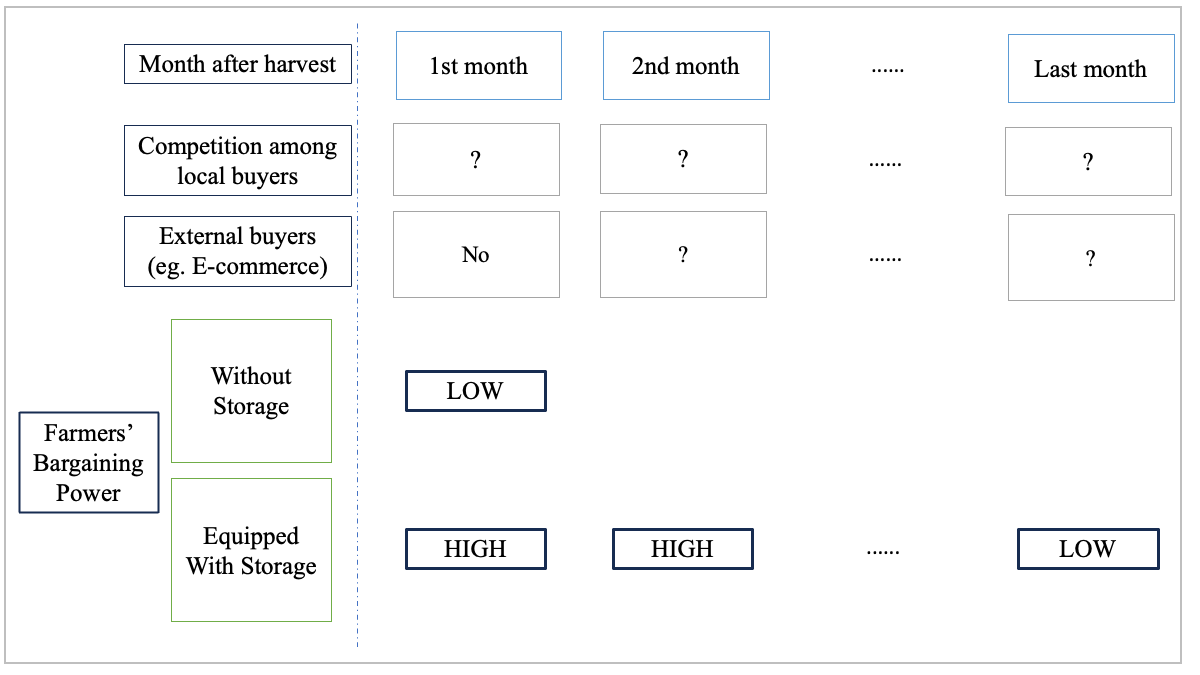
\includegraphics[width=1\textwidth]{figures/graphic_demo.png}
\caption{Extended Marketing Opportunities from Storage Adoption}
\label{Figure: Demo}
\end{figure}

Specifically, farmers could potentially benefit from increased competition in the oligopsonistic market through two sources. Firstly, the presence of different intermediaries\footnote{In this chapter, the terms middlemen, field buyers, intermediaries, and traders will be used interchangeably to refer to a group of buyers who directly purchase fresh apples from farmers. These buyers play a crucial role in the supply chain by acting as the initial link between farmers and the broader market. They typically visit orchards, negotiate prices with farmers, and handle the immediate procurement of apples. Their role may also include transporting apples to wholesale markets, processing facilities, or exporters, depending on the supply chain dynamics. Regardless of the specific term used, all these buyers share the common function of directly sourcing apples from farmers before the produce reaches larger market players, such as wholesalers, retailers, or processors.} in the village at various times can create fluctuating levels of competition on a monthly or even weekly basis. Secondly, farmers with storage can tap into additional distribution channels such as e-commerce and direct selling, which differ from the conventional middlemen-dominated system. By doing so, they can introduce external participants into the oligopsonistic market at the farm gate at different time nodes. 

I develop a conceptual framework to explore how smallholder farmers can adopt cold storage to potentially exploit the time-varying buyer power of middlemen. It considers a simplified dynamic, two-period scenario in a developing country, where farmers sell a specific cash crop to middlemen who visit local villages to procure the farm product. The model incorporates a storage-decision process, wherein farmers, observing farm-gate prices at harvest, decide whether to sell or store their crops.

The outcomes of this study hold substantial implications for policymakers and farmers alike. By exploring the dynamics of time-varying oligopsony levels, the research aims to demonstrate the potential benefits of storage facilities for smallholder producers. In a broader context, the findings suggest that embracing storage adoption could provide farmers with an effective alternative to combat anti-competitive practices like buyer collusion and market division and avoid more intrusive measures in markets, such as direct government intervention.





\section{Base Model}
\noindent I develop a two-period dynamic model to analyze how smallholder farmers strategically utilize storage in response to time-varying buyer power exerted by middlemen. The model is set in a rural area of a developing country, where farmers market a cash crop to itinerant traders. Harvest quantity is treated as exogenous, and the analysis focuses exclusively on farmers' storage and sales decisions within a single crop cycle. To identify the impact of market structure and trading dynamics, product quality is assumed homogeneous across farmers.

Farmers exhibit risk preferences ranging from risk neutrality to moderate risk aversion, valuing consumption at market prices. Each farmer is represented by a von Neumann–Morgenstern utility function,\footnote{An alternative mean-variance framework, presented in Appendix~\ref{Appendix: mean-variance approach}, yields similar insights. However, due to limited empirical guidance on calibrating the risk aversion coefficient within agricultural supply chains for the mean-variance framework, my primary analysis relies on the expected utility framework.} $U_i(\pi_i)$, with $U_i' > 0$ and $U_i'' \leq 0$, where $\pi_i$ is the farmer's net income from crop sales. Farmers aim to maximize the expected utility of income across two trading periods.

The central decision is determining the proportion of the harvest stored immediately post-harvest, denoted by $s \in [0,1]$. This choice is made under uncertainty about future market conditions, specifically future buyer power dynamics in the subsequent trading period. I will represent buyer power in each period $t$ by the parameter $\theta_t$ and will later show that we can bound $\theta_t$ in the unit interval.

In the initial trading period, farmers observe farm-gate price offers from middlemen. Based on the frequency and magnitudes of these offers, farmers infer the current buyer power. represented by $\theta_1$. Greater competition among buyers, characterized by lower $\theta_1$, correlates with higher farm-gate prices, $p_1$. Anticipating continuity in the inverse relationship between buyer power and prices across periods, farmers strategically allocate harvest between immediate sale and storage, incorporating expectations about future competition, captured by the random variable $\theta_2$.

Temporal demand variations downstream-such as seasonal consumption shifts-are presumed to be fully internalized by the market as a whole, including both farmers and intermediaries. Since intermediaries may engage in storage, anticipated demand fluctuations over the marketing season should already be reflected in the prices they offer at harvest. Accordingly, buyer power remains the primary source of intertemporal price variability in this model.

The model assumes symmetric information and negligible transaction costs in each trading period, ensuring farmers have complete and instantaneous access to prevailing farm-gate prices.

Formally, each farmer seeks to maximize expected utility over two trading periods by selecting storage share $s \in [0,1]$. Given a normalized harvest quantity $q = 1$, the optimization problem is:
\begin{equation}
\label{eq:starting objective}
\max_{s \in [0,1]} \mathbb{E} \left(U\left[ (1 - s) p_1 + s \cdot p_{2,\text{net}} \right]\right).
\end{equation}
where $p_1$ is the farm-gate price at harvest and $p_{2,\text{net}}$ is the second-period price adjusted for storage costs.



\subsection{Middlemen Market Structure and Farm-Gate Price Formation} \label{Section: Middlemen Market Structure and Farm-Gate Price Formation}
\noindent To analyze farmers' strategic use of storage as a form of intertemporal bargaining, it is essential to model farm-gate price formation in a manner that flexibly incorporates the degree of competition among middlemen.

I adopt the \textit{Flexible Oligopoly/Oligopsony Market (\textit{FOOM})} framework to model farm-gate pricing as a function of buyer market power. Under the assumption that downstream markets, wholesale or retail, where traders sell the farm products they procure, are perfectly competitive, the farm-gate price $p_{f,t}$ in each period $t$ is determined as:
\begin{equation}
p_{f,t} = \frac{p_{r,t} - mc_t}{1 + \frac{\theta_t}{\varepsilon_t}},
\end{equation}
where $p_{r,t}$ is the downstream price and $mc_t$ denotes the buyers' marginal cost in period $t$, $\theta_t$ captures the degree of buyer power in period $t$, and $\varepsilon_t$ represents the farm supply elasticity facing buyers in period $t$.\footnote{For a detailed derivation, see Appendix~\ref{Appendix: Derivation of Farm Price under the FOOM Framework}.}


For simplicity, supposing the downstream price net of marginal cost is constant across periods and normalizing it to unity ($p_{r,t} - mc_t = 1$), the farm-gate price reduces to:
\begin{equation}
p_{f,t} = \frac{\varepsilon_t}{\varepsilon_t + \theta_t}.
\end{equation}


Although total harvest quantity is fixed at the time of the first-period decision, supply in that period remains somewhat elastic due to farmers' ability to store part of their output. In period 2, supply is also elastic, as farmers can divert unsold produce to alternative buyers such as fruit-processing firms. To simplify the analysis while preserving these features, I assume a baseline supply elasticity of $\varepsilon_t = 1$ for both periods. This assumption serves as a plausible starting point and will be relaxed in subsequent analysis. Thus, farm-gate prices reduce further to:
\begin{equation}
p_{f,t} = \frac{1}{1+\theta_t}, \quad \theta_t \in [0,1],
\label{Eq: price formation by buyer power}
\end{equation}
where $\theta_t=0$ corresponds to perfect competition among buyers and $\theta_t=1$ denotes pure monopsony. Forms of oligopsony competition, such as Cournot competition, are represented by intermediate values of $\theta_t$, with higher values denoting progressively greater departures from competition \citep{karp1996dynamic,sexton2001assessment, saitone2009flexible, hamilton2021joint}.

Assuming farmers believe that this price formation rule persists across periods, period-specific prices are determined as $p_t = \frac{1}{1+\theta_t}, \quad t=1,2$. At harvest time, farmers observe $p_1$ and infer the contemporaneous buyer power, $\theta_1 = \frac{1 - p_1}{p_1}$. They then form expectations about the second-period buyer power, $\theta_2 \in [0,1]$, which is stochastic, and its distribution can be independent or based on the observation of $\theta_1$ under further assumptions. Thus, the second-period price can be expressed as:
\begin{equation}
p_2(\theta_2) = \frac{1}{1+\theta_2} 
\label{Eq: p_2 of buyer power change}
\end{equation}


To incorporate the economic cost of storage--including physical storage expenses, intertemporal discounting, and potential quality deterioration--I define the second-period price in net terms using a storage efficiency parameter $\kappa \in [0,1]$, which captures the overall storability of the commodity. Rather than modeling storage cost as a fixed deduction, I assume that storage frictions reduce the realized price proportionally, so that the farmer receives only a fraction $\kappa$ of the gross second-period price. This formulation captures a broad class of storage frictions, such as spoilage, shrinkage, and financing costs, that scale with the value of the commodity. It also reflects how farmers often perceive post-harvest losses: as a proportional reduction in potential revenue. From an analytical standpoint, the proportional specification preserves tractability under the Constant Relative Risk Aversion (CRRA) preferences, where utility is homogeneous of degree one and sensitive to relative rather than absolute changes in income. Accordingly, I define the net second-period price as:
$$
p_{2,\text{net}}(\theta_2) = \kappa \cdot p_2(\theta_2),
$$
where the gross second-period price remains $p_2(\theta_2) = \frac{1}{1 + \theta_2}$. Thus, the full expression becomes:
$$
p_{2,\text{net}}(\theta_2) = \frac{\kappa}{1 + \theta_2}.
$$
This setup ensures that the incentive to store responds coherently to economic fundamentals while allowing for an intuitive interpretation of $\kappa$: when $\kappa = 0$, the product is perfectly perishable and yields no second-period returns; when $\kappa = 1$, the product is perfectly storable with no loss in value.






\subsection{Final Objective Function}

\noindent The economic environment at harvest is summarized in Table~\ref{tab:baseline model parameter table}, capturing both observed and unobserved determinants of the farmer's storage decision over two periods.

\begin{table}[H]
\centering
\caption{Economic Environment at Harvest}
\label{tab:baseline model parameter table}
\begin{tabular}{lll}
\toprule
\textbf{Item} & \textbf{Symbol (units)} & \textbf{Status at Harvest} \\
\midrule
Harvest quantity & $q$ & Known, fixed (normalized to 1) \\
First-period price & $p_1$ & Observed \\
First-period buyer power & $\theta_1 = \frac{1 - p_1}{p_1}$ & Inferred from $p_1$ \\
Second-period buyer power & $\theta_2$ & Stochastic \\
Second-period price & $p_2 = \frac{1}{1 + \theta_2}$ & Derived \\
Storage efficiency factor & $\kappa \in [0,1]$ & Observed \\
Second-period net price & $p_{2,\text{net}} = \frac{\kappa}{1 + \theta_2}$ & Derived \\
CRRA risk aversion & $\gamma \in [0,10]$ & Observed \\
\bottomrule
\end{tabular}
\end{table}

\noindent The farmer allocates a share $s \in [0,1]$ of output to the second-period sale and retains the remainder for immediate sale at price $p_1$. Without a specific assumption on the utility functional form, substituting the expressions for $p_1$ and $p_{2,\text{net}}$, a farmer's maximization problem becomes:
\begin{equation}
\label{eq:final objective}
\max_{s \in [0,1]} \mathbb{E} \left\{U\left[\underbrace{\frac{1-s}{1+\theta_1}}_{\text{First-period income}} + \underbrace{s \cdot \frac{\kappa}{1+\theta_2}}_{\text{Adjusted second-period income}} \right]\right\}.
\end{equation}


\subsection{Risk Neutrality: Closed-Form Solution}
\noindent Under the case of risk neutrality, the utility function becomes linear: $U(\pi) = \pi$. The objective simplifies to:
\begin{equation}
\max_{s \in [0,1]} \; 
(1 - s) \cdot \frac{1}{1 + \theta_1} 
+ 
s \cdot \kappa \cdot \mathbb{E} \left[ \frac{1}{1 + \theta_2} \right].
\end{equation}
The solution simply depends on a comparison of marginal returns:
\begin{equation}
s^*( \gamma = 0) =
\begin{cases}
1 & \text{if } \kappa \cdot \mathbb{E} \left[ \frac{1}{1 + \theta_2} \right] > \frac{1}{1 + \theta_1}, \\
0 & \text{if } \kappa \cdot \mathbb{E} \left[ \frac{1}{1 + \theta_2} \right] < \frac{1}{1 + \theta_1}, \\
\text{any } s \in [0,1] & \text{if equality}.
\end{cases}
\label{Eq: risk-neutrality solution}
\end{equation}

\noindent Under risk neutrality, the farmer evaluates only expected monetary payoff. The decision reduces to a pure binary choice: if the net expected second-period price exceeds the normalized first-period price, then storage is optimal; otherwise, immediate sale dominates. Indifference arises only when the two expected returns are equal.


\subsection{Risk Aversion: Numerical Approach Needed}
\noindent In the presence of risk aversion---that is, when the utility function is strictly concave---analytical solutions to the farmer's maximization problem are generally out of reach. This intractability arises from the fact that risk aversion embeds the random second--period buyer–power shock $\theta_2$ inside a nonlinear transformation.  With a strictly concave utility function $U(\cdot)$, the marginal utility term that enters the first-order condition is $U'\!\left[\frac{1-s}{1+\theta_1}+ s\frac{\kappa}{1+\theta_2}\right]$.  Because $s$ appears both outside and inside the expectation, the optimality condition requires solving
$$
\mathbb{E}\!\left\{\,U'\!\Bigl[\cdot\Bigr]\!\left[-\frac{1}{1+\theta_1}+\frac{\kappa}{1+\theta_2}\right]\right\}=0,
$$
which is a Fredholm integral equation. For generic concave $U$ (e.g., CRRA, CARA, or quadratic utility outside the linear range), the integral has no closed-form anti-derivative, because $U'$ must be evaluated at every realization of $\theta_2$ and then averaged over its distribution. Only by imposing knife-edge assumptions---such as risk neutrality ($U''=0$), degenerate $\theta_2$, or special affine-transform utility---does the expectation reduce to an algebraic expression that can be inverted to solve for $s$.

Even when the distribution of $\theta_2$ is simple, analytic integration remains elusive. The ratio $\kappa/(1+\theta_2)$ introduces a hyperbolic term inside $U$, so the composition $U'\circ g(\theta_2)$ usually lacks a primitive.  Consequently, the derivative of the expected utility cannot be written as a finite combination of elementary functions, precluding a closed-form solution for the interior optimum. 

Moreover, the introduction of risk aversion couples the mean and higher-order moments of $\theta_2$ together. The comparative-static effects of skewness or variance on $s^{*}$ therefore enter through higher-order derivatives of $U$, which are inseparable from the integral above.  This dependence further limits traceability.


These complications drive me to employ numerical analysis, specifically, the Monte Carlo evaluation of the expectation, to approximate the optimal storage share $s^{*}$ while respecting the corner constraints $s\in[0,1]$.





\section{Numerical Analysis} \label{Section: Base Model Numerical Analysis}
\noindent To examine how risk preferences and storage efficiency shape farmers' intertemporal marketing decisions under buyer power uncertainty, I numerically solve for the optimal storage share $s^*$ across a range of parameter values. This section describes the simulation design and computational procedure employed to approximate the farmer's decision problem under Constant Relative Risk Aversion (CRRA) utility.


\subsection{Setup and Parameterization}
\noindent A farmer is assumed to observe a moderate level of first-period buyer power $\theta_1 = 0.5$, the midpoint of the support. Second-period buyer power $\theta_2$ is stochastic and modeled using Beta distributions bounded on the unit interval $[0,1]$, allowing for flexible skewness and kurtosis while maintaining economically relevant support.

I consider eight distinct Beta distributions defined by a full factorial combination of:
\begin{itemize}
\item \textbf{Four means}: $\mu_{(\theta_2)} \in {0.2,,0.4,,0.5,,0.8}$, and
\item \textbf{Two variances}: $\sigma^2_{(\theta_2)} \in {0.02,,0.05}$, representing low and high uncertainty respectively.
\end{itemize}

For each $(\mu_{(\theta_2)}, \sigma^2_{(\theta_2)})$ pair, the corresponding shape parameters $(\alpha, \beta)$ are computed using the standard moment-matching formulas:

$$
\alpha = \mu_{(\theta_2)} \left( \frac{\mu_{(\theta_2)}(1 - \mu_{(\theta_2)})}{\sigma^2_{(\theta_2)}} - 1 \right), \quad
\beta = (1 - \mu_{(\theta_2)}) \left( \frac{\mu_{(\theta_2)}(1 - \mu_{(\theta_2)})}{\sigma^2_{(\theta_2)}} - 1 \right).
$$

I simulate 2,000 independent realizations of $\theta_2$ for each Beta distribution to approximate the expectation operator in the farmer's objective function.




\subsection{Numerical Strategy}
\noindent The computational approach exploits a simplification under risk neutrality ($\gamma = 0$). In this case, the utility function becomes linear and the farmer's decision reduces to the binary rule as shown in Equation~\ref{Eq: risk-neutrality solution}.

For all $\gamma > 0$, I numerically evaluate a farmer's utility under the Constant Relative Risk Aversion (CRRA) functional form:
\begin{equation}
U(\pi)=\left\{\begin{array}{ll}
\frac{\left(\pi^{1-\gamma}-1\right)}{(1-\gamma)} & \text { if } \gamma \neq 1 \\
\ln (\pi) & \text { if } \gamma=1
\end{array},\right.
\label{eq: CRRA}
\end{equation}
where $\gamma$ denotes the coefficient of relative risk aversion, and $\pi$ represents the net income realized over two periods. 

The adoption of the Constant Relative Risk Aversion (CRRA) utility function is supported by both theoretical appeal and empirical evidence. Theoretically, CRRA maintains a constant degree of relative risk aversion across income levels, aligning with microeconomic models of choice under uncertainty. Empirically, panel data studies consistently find that the share of risky assets in household portfolios remains stable across wealth levels-even amid substantial income fluctuations-supporting the CRRA assumption \citep{Berger2020Characterizing, chiappori2011relative, zavala2024unfair}. The unitless nature of the CRRA coefficient $\gamma$ enables meaningful comparisons of risk preferences across settings and countries \citep{Szpiro1986Relative, hardaker2000some}. A recent meta-analysis by \citet{Irsova2025Relative} finds that, after adjusting for publication bias, the average coefficient of relative risk aversion centers around 1 in general economic applications and between 2 and 7 in financial contexts-figures that align closely with my field observations.

Moreover, this utility form aligns well with observed farmer behavior in regions proximate to my study sites. For example, \citet{jin2024losses} document persistent risk-averse decision-making among apple growers in areas that substantially overlap with the geographic scope of my fieldwork.


To ensure the model remains broadly applicable beyond the context of apple production, I adopt a general range for the storage efficiency coefficient, $\kappa \in [0.6, 1.0]$, in the simulations. This parameter captures the combined effects of physical quality loss, storage costs, and intertemporal discounting.

For apple growers in particular, empirical evidence suggests that postharvest quality decline is modest within a single marketing season due to the use of cold storage, implying that quality deterioration is likely minimal. Storage costs are present but not prohibitive, and the dominant component affecting $\kappa$ may therefore be discounting. Drawing on literature from developing-country settings (e.g., \cite{frederick2002time, tanaka2010risk, bauer2012behavioral, saitone2018price, Belissa2019Liquidity, liu2020delayed, Umar2025Drivers}), relevant discount rates can be substantial, yet still consistent with values that keep $\kappa$ well above 0.6. Present bias is not considered here, as intra-seasonal decisions are assumed to follow time-consistent preferences. This range thus offers a realistic and flexible foundation for analyzing storage behavior under varying economic conditions.






\subsection{Simulation Grid}
\noindent Therefore, the numerical analysis is conducted over the following two-dimensional grid:
\begin{itemize}
\item \textbf{Risk aversion}: $\gamma \in [0, 10]$, discretized over 30 evenly spaced points.
\item \textbf{Storage efficiency}: $\kappa \in [0.6, 1.0]$, discretized over 20 points.
\end{itemize}

This design spans a broad range of economically plausible values-from risk neutrality to strong risk aversion, and from low to perfect storage efficiency.

Each candidate $s$ is evaluated over the 2,000 simulated values of $\theta_2$, and the resulting utilities are averaged to approximate expected utility. The maximizer of this set yields $s^*$ for the given $(\gamma, \kappa)$ configuration.

For each grid point $(\gamma, \kappa)$, I solve the farmer's problem by computing expected utility over a discrete set of 25 candidate storage shares $s \in [0, 1]$. The optimal share $s^*$ is the value that maximizes expected utility given the simulated distribution of $\theta_2$.



\subsection{3D Visualization and Interpretation}
\noindent To present results, I construct a 4-by-4 panel as shown in Figure~\ref{Figure:3D_formulation}. The layout is organized as follows:
\begin{itemize}
\item \textbf{Top and bottom rows} plot the probability density functions (PDFs) of the eight Beta distributions used to simulate $\theta_2$. Each panel is annotated with its corresponding $(\mu_{(\theta_2)}, \sigma^2_{(\theta_2)})$ and the implied $(\alpha, \beta)$.
\item \textbf{Middle two rows} display 3D surfaces of the optimal storage share $s^*$ as a function of $\gamma$ and $\kappa$, separately for low-variance (second row) and high-variance (third row) distributions.
\end{itemize}
Each 3D plot is rendered with a consistent viewing angle such that the origin, corresponding to the lowest values of both $\gamma$ and $\kappa$, appears closest to the observer. These simulation surfaces depict key mechanisms driving intertemporal storage and marketing choices under local market-structural uncertainty in agriculture.

\begin{figure}[ht!]
\centering
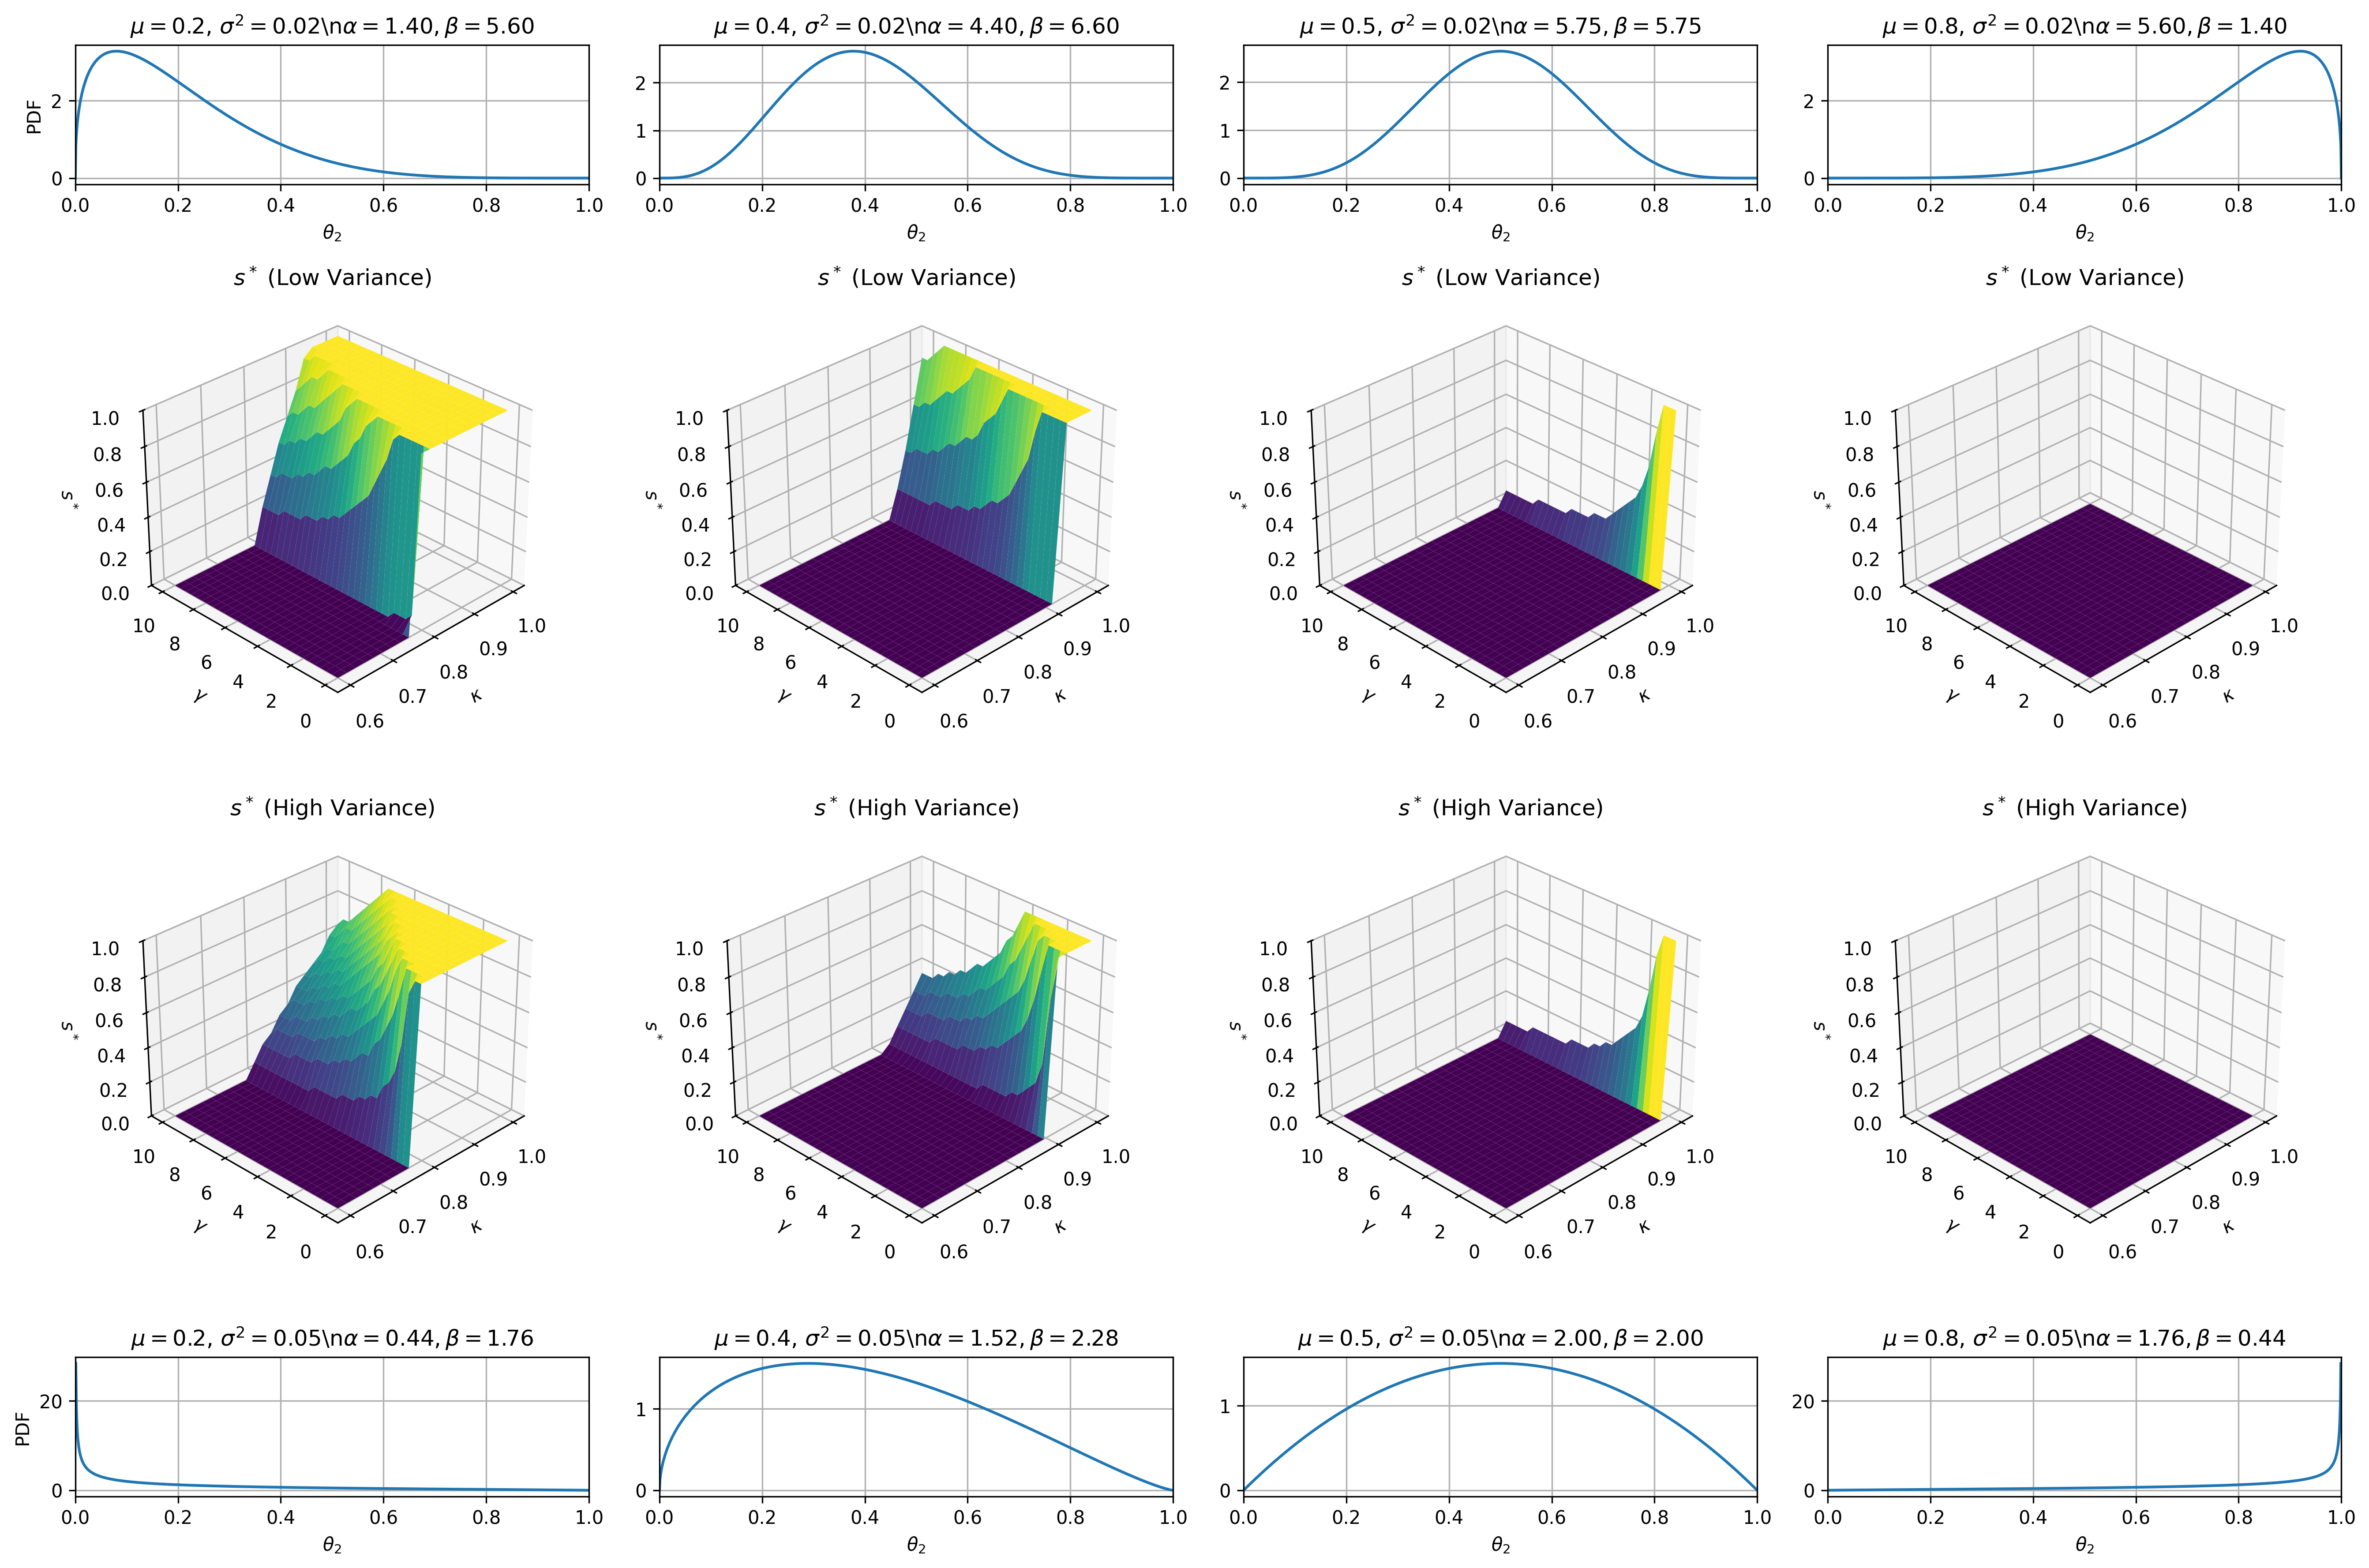
\includegraphics[width=\textwidth]{model_figures/3D_formulation.png}
\caption{Optimal Storage Share and PDF Visualizations under Eight Beta Distributions of $\theta_2$}
\label{Figure:3D_formulation}
\end{figure}

In general, when the farmer expects buyer power to be stronger in the future than at harvest-that is, when $\mathbb{E}[\theta_2] > \theta_1$-the incentive to store totally disappears. In other words, farmers would never store when $\mu > 0.5$ in our simulation here. As illustrated in the far-right column of the panel, the optimal strategy across all risk and efficiency levels is to sell immediately ($s^* = 0$).

In contrast, when expectations about future buyer power are neutral or favorable ($\mathbb{E}[\theta_2] \leq \theta_1$), the decision becomes more nuanced. Interior solutions ($0 < s^* < 1$) emerge over a meaningful range of risk preferences and storage efficiencies. Moreover, as the expected buyer power $\mathbb{E}[\theta_2]$ declines, both the scope for interior solutions and the frequency of corner solutions with full storage ($s^* = 1$) expand, reflecting the improved relative attractiveness of deferring sales.



Within each simulated surface, $s^*$ is non-increasing in $\gamma$. This pattern is especially pronounced when future buyer power is moderate-that is, when expected second-period prices are only marginally higher than those in the first period. The underlying mechanism is intuitive: risk-averse farmers increasingly value certainty over potentially higher but uncertain future payoffs. As $\gamma$ rises, the disutility associated with price risk begins to outweigh the intertemporal arbitrage opportunity, especially when those gains are compressed by relatively high buyer power.



In contrast, storage efficiency $\kappa$ plays a reinforcing role. For a given level of risk aversion, increases in $\kappa$ make storage more attractive by reducing the effective cost of waiting. Accordingly, $s^*$ is non-decreasing in $\kappa$. The responsiveness of $s^*$ to $\kappa$ weakens at higher values of $\gamma$, suggesting that even highly efficient storage systems cannot fully offset the behavioral costs of risk exposure when farmers are strongly averse to uncertainty. 


Cross-panel comparisons further illustrate how changes in the distribution of second-period buyer power affect storage incentives. As the mean future buyer power $\mu_{(\theta_2)}$ increases (moving left to right across the panels), expected second-period prices decline, rendering storage less attractive in expected-value terms. Accordingly, the optimal storage share $s^*$ shifts downward across the entire surface. This effect is especially pronounced for risk-neutral or mildly risk-averse farmers, who condition decisions almost exclusively on expected returns. The lower the expected future price, the more immediate sale becomes the dominant strategy.



Variance in buyer power exerts a subtler influence. Comparing the second and third rows of the panel-low versus high variance cases-reveals that higher variance uniformly depresses $s^*$ across all parameter combinations. This effect reflects classical prudence: with concave utility, the marginal value of additional expected income diminishes in the presence of risk. Even when the expected second-period price remains high, increased dispersion in outcomes drives down the attractiveness of storage. The effect is pronounced at intermediate levels of $\gamma$, where farmers are sensitive to risk but not yet entirely averse to delayed selling.


\subsection{Rarity of Interior Solutions}
Interior solutions, where the farmer chooses to allocate positive fractions of the harvest to both the first and second periods, are theoretically rare in this model, tested from the simulation above. The logic is straightforward: when the intertemporal trade-off is starkly tilted in favor of one period (either due to price certainty, extreme risk preferences, or inefficient storage), the farmer's best response is to sell all in one period. This is consistent with fieldwork evidence in the fresh apple industry in Central China: most apple growers tend to make corner decisions, either storing nearly everything when they expect future prices to be favorable, or selling everything immediately when uncertainty or storage cost dampens the incentive to wait. Within the model, such corner solutions arise from the nonlinearity of the CRRA utility function combined with the hyperbolic dependence of price on buyer power, which amplifies small differences in expectations or attitudes into decisive action.

To better understand the conditions under which interior solutions might arise, I extract a few representative cases from the simulation results shown in Figure~\ref{Figure:3D_formulation}. These examples are selected from scenarios with low variance in second-period buyer power and a low mean, specifically $\mu = 0.2$, where the distribution of future prices is skewed toward favorable outcomes. We restrict attention to moderate levels of risk aversion and relatively high storage efficiency, where neither risk nor cost fully dominates the farmer's decisions.

The first case features a farmer with a risk aversion coefficient around $\gamma = 2$, a storage efficiency of $\kappa \approx 0.8$, and an expected buyer power of $\mu = 0.2$. Here, the farmer chooses to store approximately 80\% of the harvest. The low expected buyer power implies a high expected price in the second period, while the relatively efficient storage technology ensures that much of this value is preserved. The farmer, though risk averse, finds it worthwhile to defer income but hedges by selling a small portion immediately. This behavior aligns well with farmers who have moderate patience and risk tolerance and access to good post-harvest storage infrastructure.

In the second case, the risk aversion parameter rises to $\gamma \approx 2.75$, with all other conditions held constant. The optimal storage share drops to about 62.5\%. The higher risk aversion amplifies the farmer's sensitivity to downside risk in second-period prices, even though the mean is favorable. The farmer still stores the majority, but the share sold in the first period increases. This behavior exemplifies a more cautious farmers who hedge against worst-case outcomes even when market fundamentals appear strong.

The third case I select maintains the same level of risk aversion as in the second case ($\gamma \approx 2.76$) but reduces the storage efficiency to $\kappa \approx 0.68$. Under these conditions, the optimal storage share drops to roughly 45.8\%. The decline in $\kappa$ reduces the effective return to deferred sales, making immediate selling relatively more attractive. This farmer, facing the same preferences and expectations as in the previous case, responds not to belief or attitude but to technical constraint. It reflects real-world circumstances where storage facilities are substandard or subject to losses from spoilage, pests, or theft-conditions that naturally discourage holding output even among patient, forward-looking producers.

Together, these three cases illustrate the sharp responsiveness of the storage decision to both preferences and storage costs. As risk aversion increases, storage declines, all else equal. And for a fixed level of risk aversion, lower storage efficiency can easily shift the farmer from a moderately storage-heavy strategy to one that leans toward immediate sale. Crucially, these interior solutions emerge only under a narrow configuration of parameters: relatively favorable and stable expectations, moderate caution, and at least tolerable storage conditions. Once any of these dimensions shifts toward uncertainty, risk aversion, or storage economic inefficiency, the solution quickly reverts to a corner.

In summary, interior solutions occur only when multiple forces---expected price gains, risk preferences, and storage efficiency---are delicately balanced. These cases are not typical but represent transitional zones in the farmer's decision space. Their rarity in both theory and field data affirms the robustness of the model's prediction: for most farmers, especially under poor storage conditions, decisive corner choices are the norm.




\subsection{Sensitivity: Expected Future Buyer Power and Risk Aversion}
\noindent To further examine how a farmer's optimal storage share $s^*$ responds to varying expectations about future buyer power, I conducted a simulation with the same parameter setting as in the 3D graphics above by holding first-period buyer power fixed at $\theta_1 = 0.5$, with a storage efficiency of $\kappa = 0.9$. The second-period buyer power $\theta_2$ was modeled as a Beta-distributed random variable with support on $[0, 1]$, maintaining a fixed variance of 0.02 while allowing the mean to vary from 0.05 to 0.95. For each mean value, I derived the associated Beta shape parameters and simulated 5,000 draws of $\theta_2$. The optimal storage share was then computed by maximizing expected utility under CRRA preferences, evaluated across five levels of risk aversion: $\gamma \in \{0, 0.5, 2, 4, 7\}$. As shown in Figure~\ref{Figure: sensitivity to second-period buyer power}, each resulting function $s^*(\mathbb{E}[\theta_2])$ was plotted to visualize how forward-looking uncertainty and risk preferences jointly shape storage behavior. Line color was varied monotonically with $\gamma$, increasing in darkness as risk aversion intensified.

The results reveal a distinct shift in behavior across risk preference levels. Under risk neutrality ($\gamma = 0$), the decision rule is binary: the farmer stores all output if the expected net-storage-cost second-period price exceeds the current one, and none otherwise. As $\gamma$ increases to positive values, the decision becomes more nuanced. The sharp threshold gradually turns into a smooth, decreasing function of $\mathbb{E}[\theta_2]$, with interior solutions appearing when the expected future buyer power is only marginally lower than the first-period one.


With higher risk aversion (like $\gamma = 4$ and $\gamma = 7$), the willingness to store declines substantially. Even when the expected second-period price exceeds today's price, the farmer often chooses to sell immediately due to the downside risk embedded in the distribution of $\theta_2$. The curve $s^*(\mathbb{E}[\theta_2])$ flattens near zero, and the turning point at which storage becomes attractive shifts leftward. This leftward shift reflects a heightened preference for certainty: more favorable expectations are required before any intertemporal transfer of output becomes worthwhile. 


\begin{figure}[ht!]
\centering
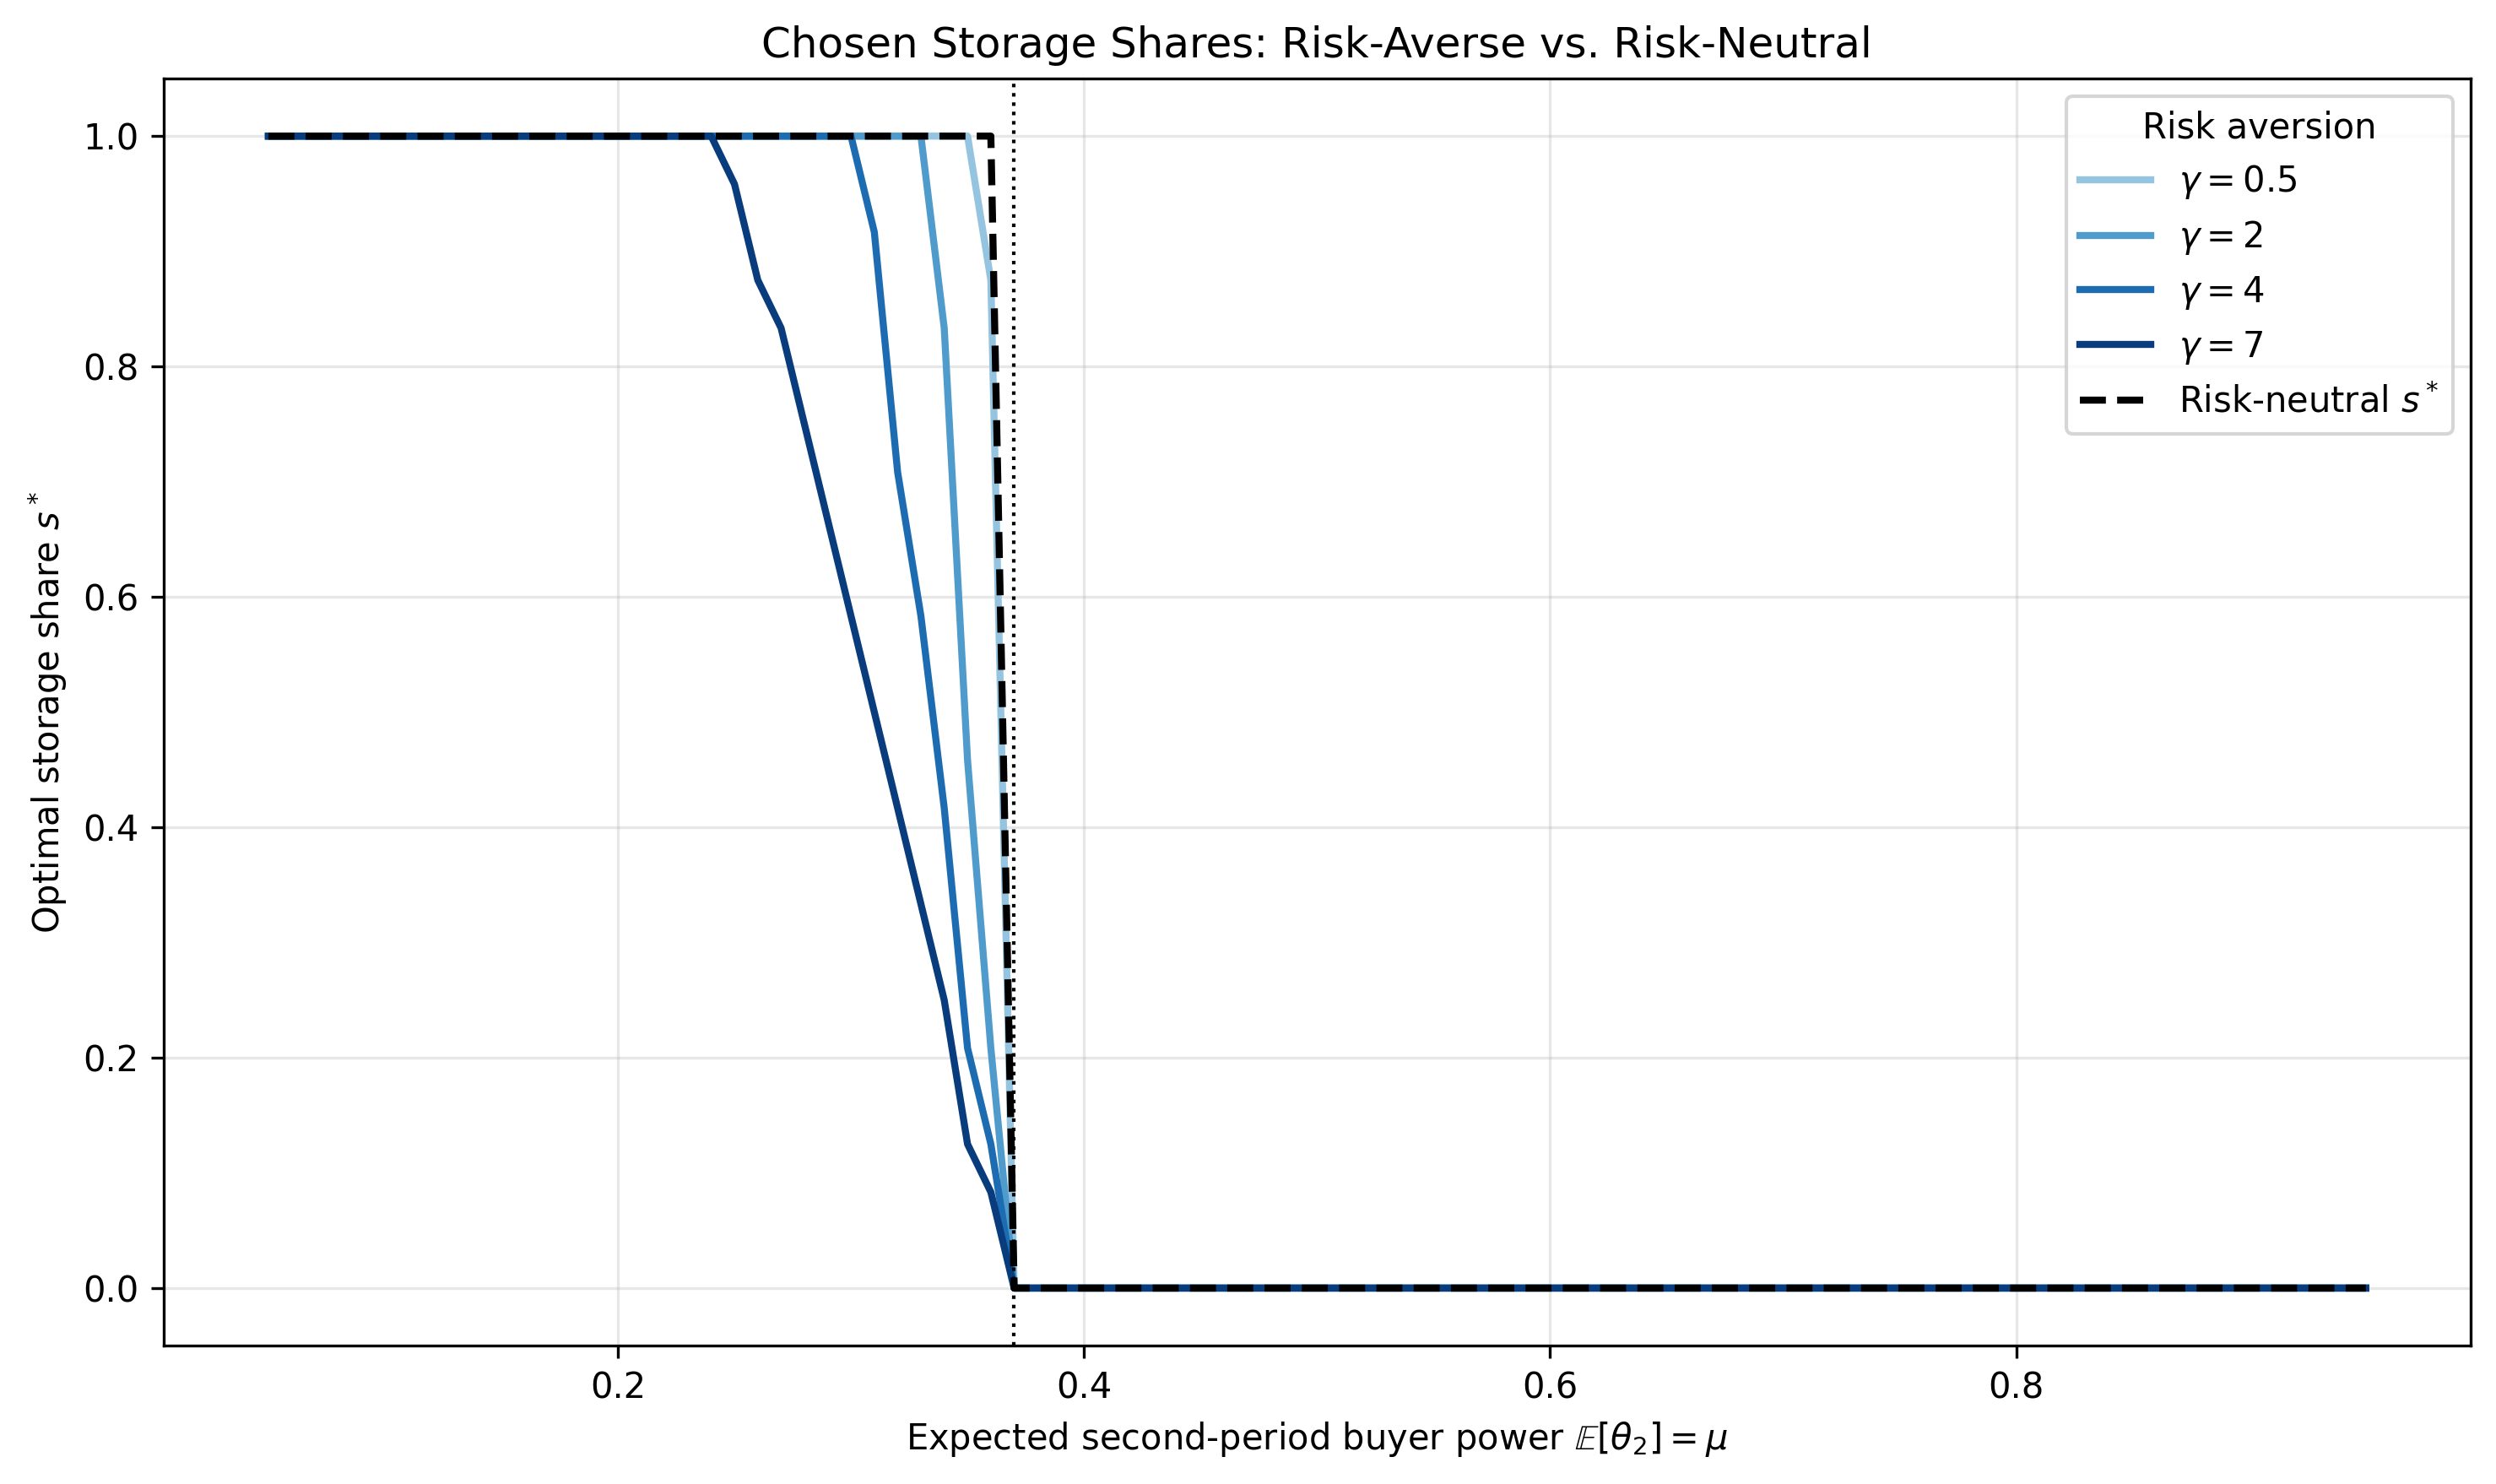
\includegraphics[width=\textwidth]{model_figures/sensitivity_to_theta_2.png}
\caption{Sensitivity to Expected Second-Period Buyer Power}
\label{Figure: sensitivity to second-period buyer power}
\end{figure}

\begin{figure}[ht!]
\centering
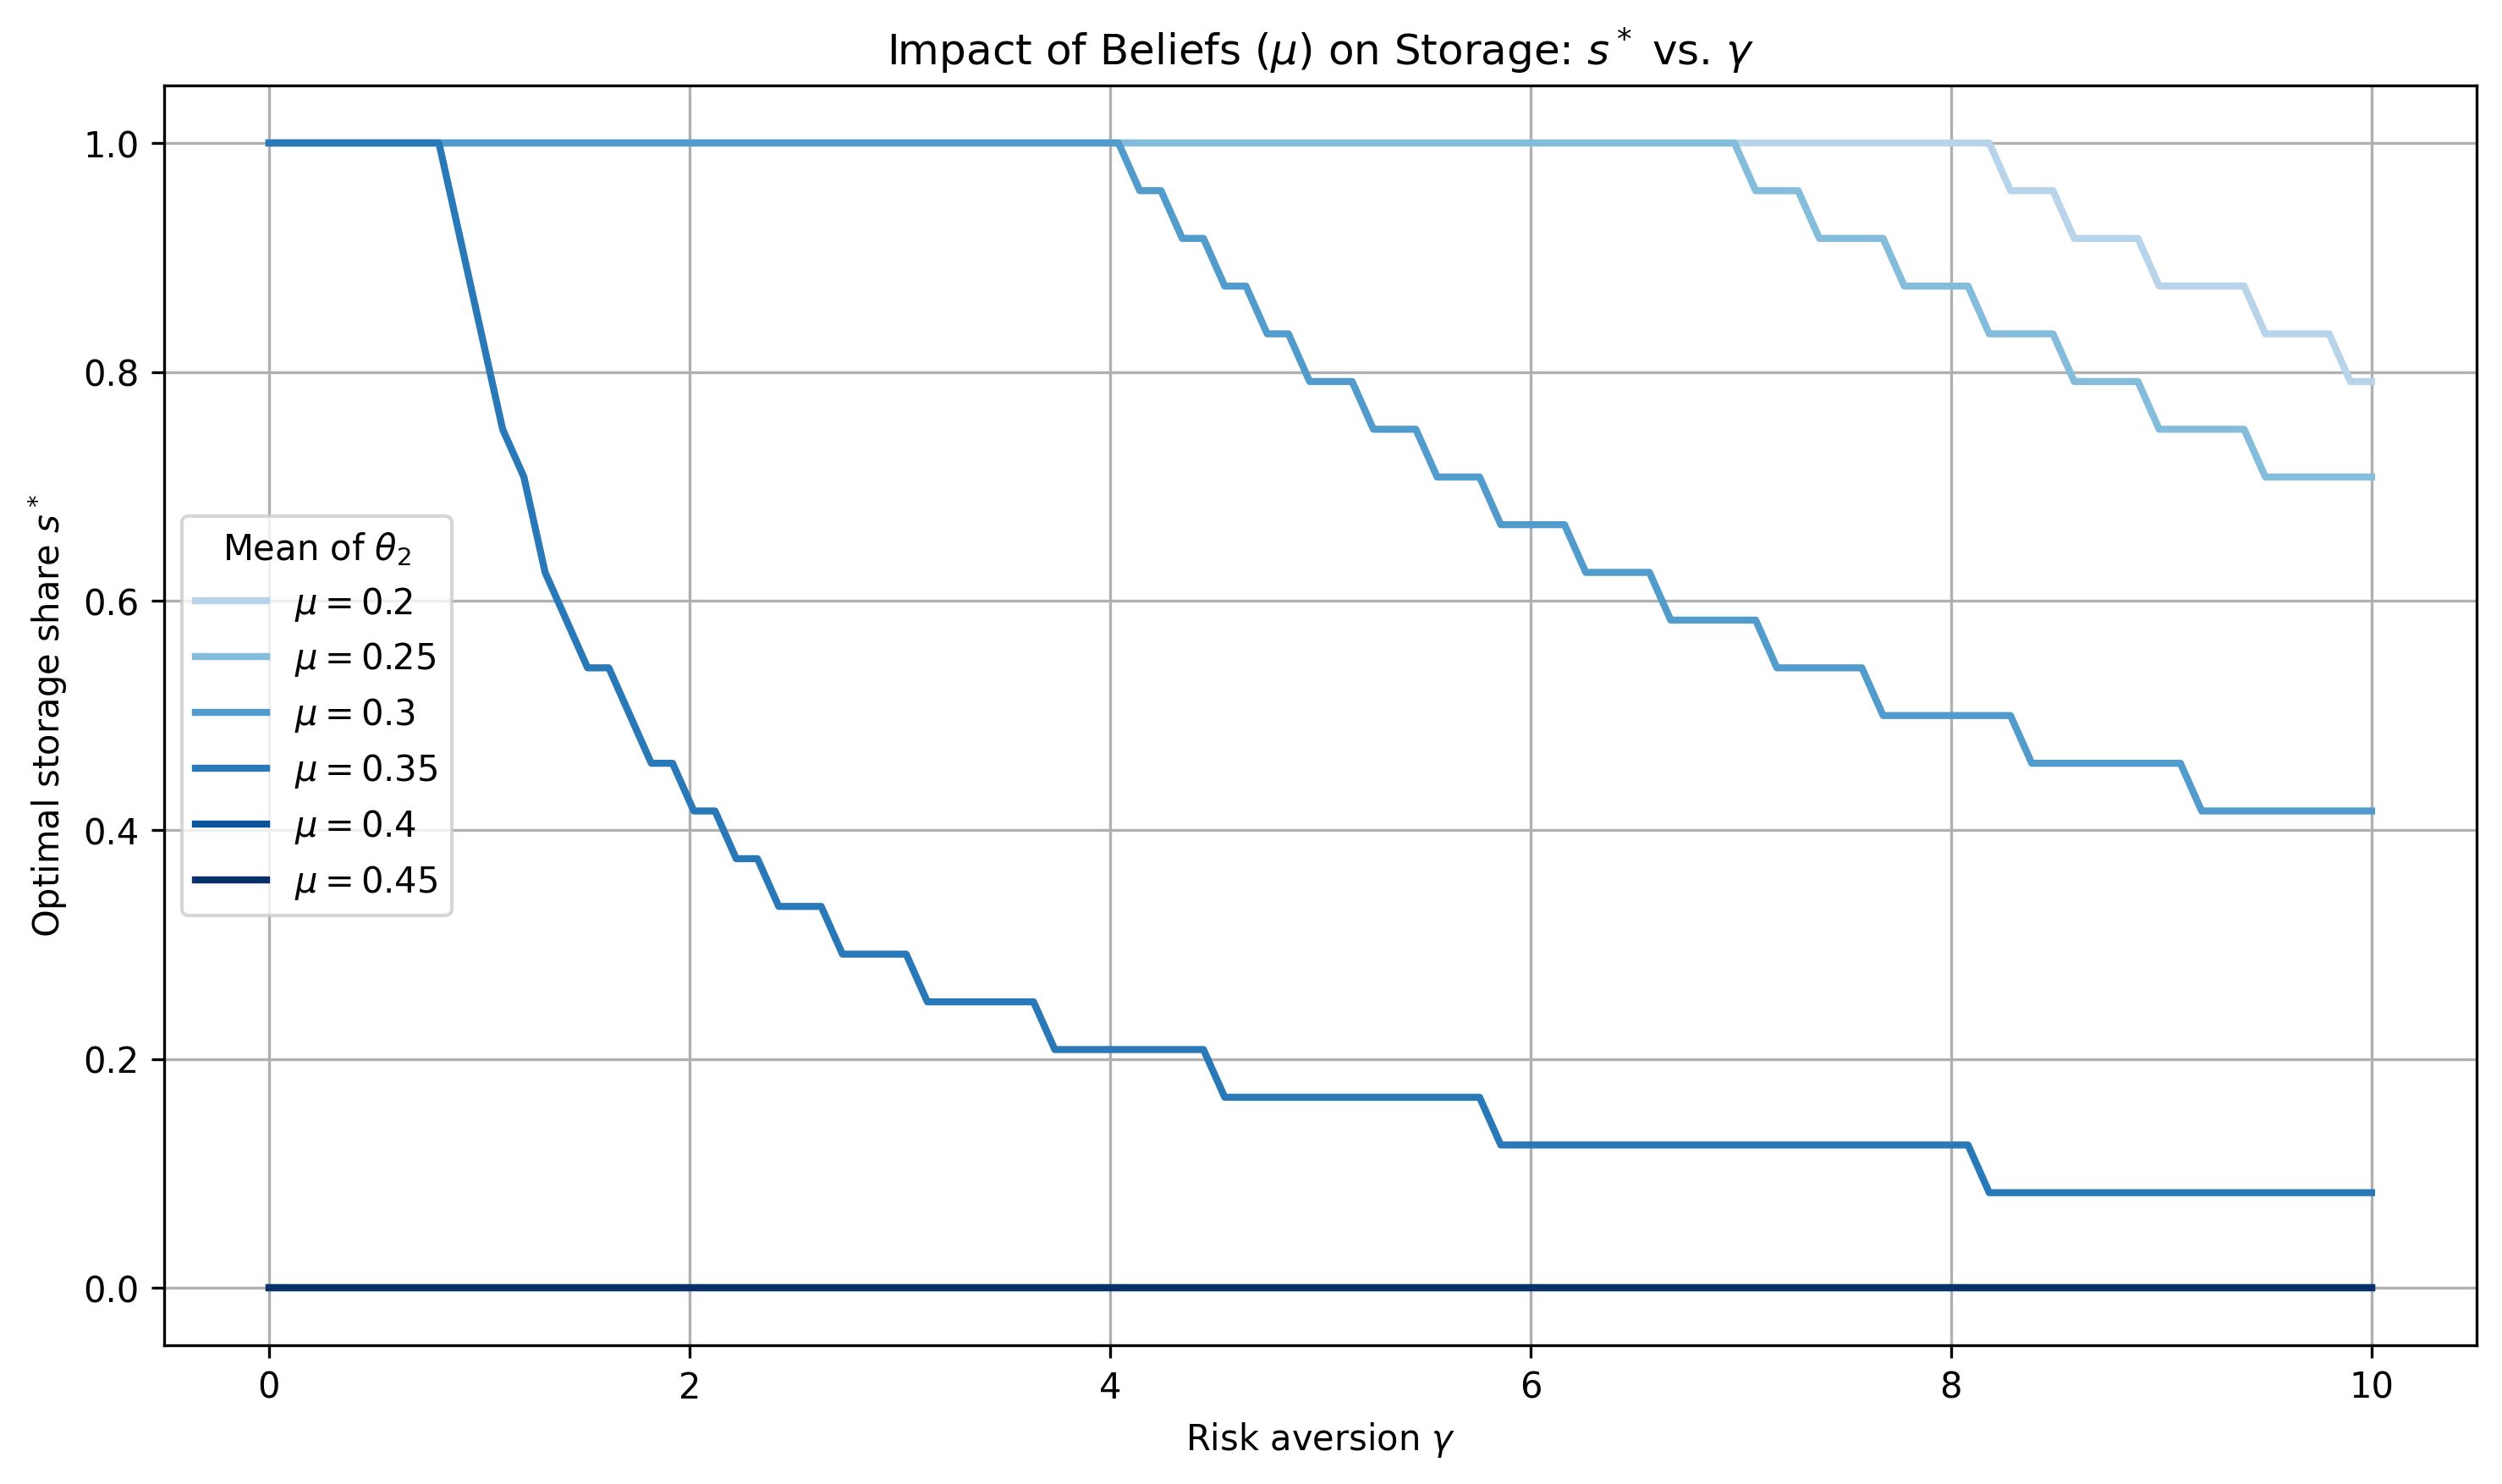
\includegraphics[width=\textwidth]{model_figures/sensitivity_to_gamma.png}
\caption{Sensitivity to Risk Aversion}
\label{Figure: sensitivity to risk aversion}
\end{figure}


In addition, I constructed another visualization in Figure~\ref{Figure: sensitivity to risk aversion} that examines how a farmer's optimal storage share responds to changes in risk aversion, under varying expectations about future buyer power. With the same parameter setting as in the 3D graphics above, I simulate buyer power beliefs using Beta distributions with means ranging from $\mu = 0.2$ to $\mu = 0.4$ in increments of 0.05. For each mean, I compute the corresponding shape parameters $(\alpha, \beta)$, draw 5,000 samples of $\theta_2$, and evaluate the expected utility under a CRRA utility function across 100 grid points of $\gamma \in [0, 10]$. The optimal storage share $s^*$ is computed by maximizing the expected utility over a grid of candidate values $s \in [0, 1]$, reflecting the proportion of harvest stored for second-period sale. Also, Figure~\ref{fig:unified_gap_plot}, discussed later in policy implications, quantifies the income consequences of risk aversion, showing both the absolute and proportional losses relative to the risk-neutral benchmark across the range of expected buyer power.



The resulting graph in Figure~\ref{Figure: sensitivity to risk aversion} plots $s^*$ against $\gamma$ for each value of $\mu$. Several patterns emerge clearly. First, storage shares are strictly decreasing in risk aversion: as farmers become more risk-averse, they prefer to sell more in the first period to avoid future price uncertainty. This is consistent with economic intuition, as risk aversion amplifies the penalty on uncertain second-period income. Second, higher expected buyer power in the second period (i.e., higher $\mu$) uniformly depresses the storage share. When future market power is expected to be strong (i.e., lower $p_2$), forward sales become less attractive, reinforcing the incentive to sell early regardless of risk preferences.

Interestingly, the sensitivity of $s^*$ to $\gamma$ becomes more pronounced as $\mu$ approaches $\theta_1$. For low $\mu$ (e.g., 0.2), storage is generally preferred---even by highly risk-averse farmers---because the expected second-period price is high. For higher $\mu$ values (e.g., 0.4), the curves flatten at lower levels of $s^*$, showing that even less risk-averse farmers opt for immediate sale under pessimistic price expectations.

This graphical structure complements prior results showing $s^*$ as a function of $\mu$ at fixed $\gamma$. Together, they offer a two-dimensional understanding of farmer behavior: beliefs about future buyer power shift the entire $s^*(\gamma)$ curve, while changes in risk aversion tilt its shape. These patterns are particularly relevant for understanding heterogeneous storage behavior across farmers who face similar market fundamentals but differ in attitudes toward risk or expectations about downstream market structure.



\section{Special Cases: Explicit Competition Forms}
\noindent In the base framework, buyer power was represented in a reduced-form manner typical of \textit{FOOM} models, where buyer power $\theta$ was treated as a latent, abstract variable inferred from observed farm-gate prices through a nonlinear transformation. Conceptually, $\theta$ can be thought of as a sufficient statistic for market structure and conduct: at one extreme, it may correspond to the number of downstream buyers $N$ (with higher $N$ implying weaker buyer power), while more generally it can capture the distribution of buyer market shares as well as the intensity of competition. For example, a low $\theta$ could reflect either many symmetric buyers competing aggressively, or a few large buyers that nonetheless compete rather than collude; conversely, a high $\theta$ could arise from concentrated market shares, tacit collusion, or explicit coordination. 

To move beyond this abstraction, I now introduce explicit models of non-cooperative buyer competition---namely, Bertrand (price-setting) and symmetric-buyer Cournot (quantity-setting) frameworks---thus ignoring for this analysis possible buyer collusion. These models provide structural microfoundations for $\theta$ by linking it to primitive features of market structure and strategic interaction.


Suppose farmers observe the number of buyers present in the village at harvest time in the first period, denoted by $N_1$, and form expectations about buyer presence in the second period, $\mathbb{E}[N_2]$. The number of buyers in each period is a discrete variable bounded between zero and a finite upper limit.

Bertrand and Cournot models offer contrasting benchmarks for non-cooperative buyer behavior. In the classic Bertrand setting, even a small number of buyers (as few as two) can generate highly competitive outcomes, a result often referred to as the ``Bertrand paradox.'' Translated into the present framework of traders purchasing from farmers, this implies that competition among a small set of buyers is sufficient to bid up the farm-gate price to the competitive benchmark---namely, the crop's \textbf{net marginal value product}, which by normalization equals 1.0 in the base model. In contrast, under Cournot competition the relationship between the number of buyers $N$ and the equilibrium farm-gate price is more gradual: as $N$ increases, buyer market power declines smoothly, and the farm-gate price converges to the competitive benchmark only asymptotically as $N \to \infty$.


To ground the discussion, I draw on my fieldwork among apple growers in Yanchang County, Central China, during the 2024–2025 agricultural year. According to my survey of the targeted 15 buyers, including the top five most influential local traders, the number of buyers visiting a village at harvest ranges from zero in remote areas to a maximum of nine.\footnote{In Figure~\ref{Figure: buyer count at harvest}, 26\% of farmers appear to forecast fewer than zero buyers in the future, which is clearly nonsensical. This artifact arises because my sample of 15 buyers does not exhaustively cover the entire population of potential buyers, only the majority of the most frequently observed ones. Hence, farmers expressing highly pessimistic expectations experienced buyer visits from buyers outside my sample.} The mean first-period buyer count is 3.34, with a median of 3. As shown in Figure~\ref{Figure: buyer count at harvest}, fewer than 7\% of surveyed growers reported no buyer presence during harvest (for simplicity, the Bertrand analysis excludes this case), while over 80\% experienced at least two buyer visits. Most farmers reported between two and five buyers, motivating my assumption of a Poisson distribution for second-period buyer counts in the Cournot analysis.

Importantly, farmers' expectations about second-period buyer presence appear weakly correlated with observed first-period buyer counts. This is illustrated by the color segments within each bar in Figure~\ref{Figure: buyer count at harvest}, which show considerable heterogeneity in forward-looking beliefs conditional on current buyer exposure.

\begin{figure}[ht!]
\centering
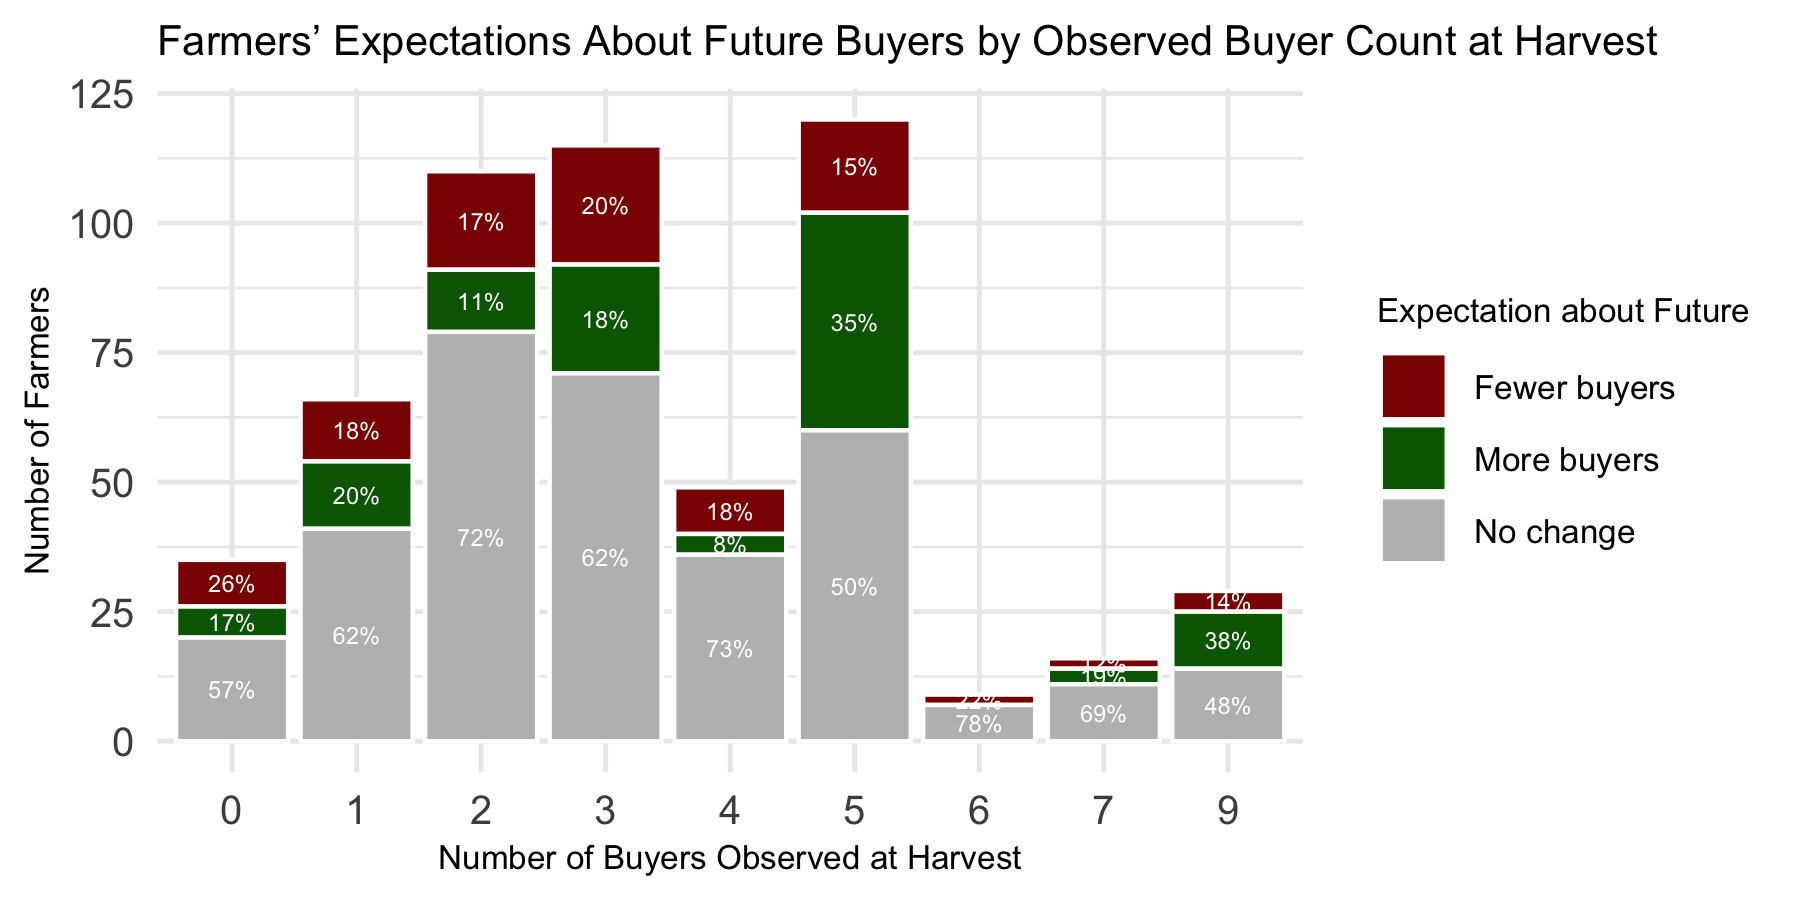
\includegraphics[width=\textwidth]{figures/buyer_count_distribution.png}
\caption{Observed Buyer Count at Harvest with Farmers' Expectations About Future Buyers}
\label{Figure: buyer count at harvest}
\end{figure}


\subsection{Price-Setting Competition: Bertrand--Nash Equilibrium}
\noindent In the price-setting environment, buyers set the price they offer to farmers. If there are no capacity constraints, the standard Bertrand logic applies: even two buyers suffice to drive the purchase price up to the competitive benchmark, which is normalized to 1 under our derived price formation rule in Equation~\ref{Eq: price formation by buyer power}. This outcome, often referred to as the Bertrand Paradox, corresponds here to a Bertrand--Nash equilibrium in which perfectly competitive outcomes ($\theta_t=0$) arise as long as $N_t \geq 2$.

Therefore, under Bertrand conditions, according to Equation~\ref{Eq: price formation by buyer power}, the farm-gate price received by farmers can be modeled as:
\begin{equation}
p_t = 
\begin{cases}
0.5, & N_t = 1 \\
1, & N_t \geq 2
\end{cases}
\label{Eq: Bertrand Price Schedule}
\end{equation}
\noindent where $0.5$ denotes the monopsonistic price paid when only one buyer is present. The transition from a single-buyer market to a multi-buyer market results in a discontinuous shift in price.

Here, I assume that farmers observe the first-period price at harvest, and the number of traders at a specific village in the second trading period ($N_2$) is stochastic, with the probability of one middleman being $\rho$, i.e., $Pr(n_2=1)=\rho$. So, the probability of multiple intermediaries appearing in village $j$ is $Pr(n_2 \geq 2) = 1-\rho$. One plausible explanation for the temporal variation in buyer presence is the buyers' limited logistical capacity, such as a shortage of trucks or prohibitive transportation costs, which prevents them from visiting every village \citep{jung2022structural}. Another factor could be collusion among traders, leading to the allocation of markets, turning each trader into a monopsony in their assigned markets during the designated periods \citep{herings2005intertemporal}. However, collusion is prone to breakdowns, as cartels are inherently unstable. Therefore, even if trader collusion occurs in period 1, it may not persist into period 2.

Therefore, a farmer's optimization problem in Equation~\ref{eq:final objective} could be written as follows:
\begin{equation}
\max_{s \in [0,1]} \psi(\cdot) = \rho U((1-s)p_1 + \kappa s \cdot 0.5) + (1-\rho) U \left( (1-s)p_1 +  \kappa s \cdot 1 \right)
\end{equation}
where the first expression on the right-hand side reflects the utility from storing $s$ share of production to the second period in the monopsonistic case, and the second term represents the utility in the case of perfect competition among buyers. 

Since all farmers would sell immediately at harvest when multiple buyers are present ($p_1 = 1$), the problem can be further simplified by setting the first-period price as the monopsonistic price ($p_1 = 0.5$), yielding:
\begin{equation}
\label{eq:Bertrand objective}
\max_{s \in [0,1]} \psi(\cdot) = \rho U((1-s)\cdot0.5 + \kappa s \cdot 0.5) + (1-\rho) U \left( (1-s)\cdot0.5 +  \kappa s \cdot 1 \right)
\end{equation}

Differentiating Equation~\ref{eq:Bertrand objective} with respect to $s$ gives the marginal utility gain from reallocating one unit of output from immediate sale to storage:

\begin{equation}
g(\cdot) = \frac{d\psi}{ds} = \rho U^{\prime}(\pi_L(s)) \cdot 0.5(\kappa-1) + (1 - \rho) U^{\prime}(\pi_H(s)) \cdot (\kappa-0.5)
\label{Eq: bertrand FOC}
\end{equation}
where $\pi_L(s) = (1 - s)\cdot 0.5 + \kappa s \cdot 0.5$ and $\pi_H(s) = (1 - s)\cdot 0.5 + \kappa s$ denote net income under low and high second-period prices, respectively.

Evaluated at $s = 0$-i.e., no storage-the marginal utility becomes:
$$
\left.\frac{d\psi}{ds}\right|_{s=0} = U^{\prime}(0.5) \cdot \left[\kappa(1 - 0.5\rho ) - 0.5\right]
$$
The bracketed term reflects the expected second-period price, net of storage loss. Since $U'(\cdot) > 0$, the sign of this expression determines whether storing is utility-improving. In particular, the farmer finds storage profitable ($s^* > 0$) if and only if:
$$
\kappa(1 - 0.5\rho) > 0.5
$$
That is, expected gains from delayed sale, adjusted for storage inefficiency, must exceed the current price. If this inequality holds, deviating from zero storage increases expected utility. Then we can derive the following three lemmas:
\begin{lemma}
    The condition $\kappa (1 - 0.5\rho) < 0.5$ is necessary and sufficient for the farmer to sell the entire harvest in the first period, $s^*=0$.
        \label{lemma: Bertrand no storage solution}
\end{lemma}
\begin{proof}
    From Equation~\ref{Eq: bertrand FOC}, we can derive the second-order condition $\frac{d^2 \psi}{d s^2} = \rho U^{\prime \prime}\left(\pi_L(s)\right) \cdot\left(-0.5+ \kappa \cdot 0.5\right)^2+(1-\rho) U^{\prime \prime}\left(\pi_H(s)\right) \cdot\left(-0.5+\kappa\right)^2$. Since $U^{\prime\prime}(\cdot)\leq0$, the entire RHS expression is non-positive. Therefore, when $\kappa (1-0.5\rho) < 0.5 $, the $\frac{d \psi(s=0)}{d s}$ would never be positive.
\end{proof}


\begin{lemma}
    On the contrary, when $\kappa (1-0.5\rho) > 0.5 $ and $\frac{d \psi(s=1)}{d s}>0$, then the farmer maximizes utility by storing the entire harvest for second-period sale, $s^*=1$.
    \label{lemma: Bertrand full storage solution}
\end{lemma}
\begin{proof}
    As $\kappa (1-0.5\rho) > 0.5 $ secures a positive storage share proven above, $\frac{d \psi(s=1)}{d s}>0$ ensures that expected utility is increasing in $s$. Therefore, at any given point of $s$, it would be optimal for the farmer to store more to get higher utility till $s$ reaches its upper bound.
\end{proof}


\begin{lemma}
    A farmer optimally adopts partial storage strategy (i.e., marketing production through both periods, $s^*\in (0,1)$) when the conditions $g(\cdot)  =  \frac{d \psi}{d s} = 0$ and $g^\prime(\cdot) = \frac{d^2 \psi}{d s^2} < 0 $ (implying a strictly risk-averse farmer), are satisfied in the range $0<s<1$.
    \label{lemma: Bertrand Interior solution}
\end{lemma}
\begin{proof}
    This is a standard interior optimum: the first-order condition holds and the second-order condition ensures a local maximum. Strict risk aversion ($U^{\prime\prime} < 0$) guarantees concavity and uniqueness.
\end{proof}

These three lemmas establish a complete characterization of the farmer's storage behavior under monopsony at harvest ($p_1 = 0.5$): sell immediately, store fully, or split output across periods.  

Under monopsonistic first-period pricing, local comparative statics can be derived using the implicit function theorem. Let $g(s) = \frac{d\psi}{ds}$ denote the first-order condition for interior optimality. Then for any parameter $\xi \in {\rho, \kappa}$, the sensitivity of the optimal storage share satisfies:
$$
\frac{\partial s^*}{\partial \xi}= -\frac{\frac{\partial g}{\partial \xi}}{\frac{\partial g}{\partial s}}
$$
Since the second-order condition ensures $\partial g / \partial s = \frac{d^2\psi}{ds^2} < 0$, the sign of $\frac{\partial s^*}{\partial \xi}$ is governed by the sign of $\partial g / \partial \xi$. Hence, storage is increasing in storage efficiency factor $\kappa$-where lower storage cost unambiguously increases storage. However, the comparative statics with respect to $\rho$ is not signed deterministically. This limits the interpretive power of local sensitivity analysis, especially given the narrow parameter region where an interior solution $s^* \in (0,1)$ arises, as shown in the previous section.







\subsection{Quantity-Setting Competition: Cournot--Nash Equilibrium}
\noindent In the quantity-setting environment, each homogeneous buyer simultaneously chooses a purchase quantity, taking others' decisions as given. The resulting Cournot–Nash equilibrium reflects strategic quantity-setting behavior. Unlike in the Bertrand case, prices are not binary but vary smoothly with the number of active buyers.

Maintaining the linear demand structure introduced in Equation~\ref{Eq: price formation by buyer power}, the farm-gate price in each period $t$ under quantity-setting competition is given by:
\begin{equation}
p_t = \max\left\{\frac{N_t}{N_t + 1}, \underline{p} \right\}, \quad t = 1,2,
\end{equation}
where $N_t \in \mathbb{N}_0$ denotes the number of standard fresh-fruit buyers in period $t$, and $\underline{p} \in (0,0.5)$ represents the low reservation price offered by fallback channels-typically processing facilities that accept any produce regardless of quality, but at steeply discounted rates. When at least one standard buyer is active ($N_t \geq 1$), the equilibrium price is strictly increasing in $N_t$, approaching the competitive limit of 1. When no such buyers are present ($N_t = 0$), the farmer receives $\underline{p}$ by selling to the outside option.

This formulation ensures continuity of the farmer's problem and captures the floor imposed by fallback markets. Although Figure~\ref{Figure: buyer count at harvest} includes a small number of reported instances with zero buyers, these are likely due to limitations in survey coverage, which focused on 15 standard fresh-fruit buyers and may have missed informal or processors' purchasing activity.

Accordingly, the farmer's maximization problem under Cournot competition becomes:
\begin{equation}
\label{eq:Cournot objective function}
\max_{s \in [0,1]} \mathbb{E} \left\{ U \left[ 
\underbrace{(1-s) \cdot p_1(N_1)}_{\text{First-period income}} 
+ \underbrace{s \cdot \kappa \cdot p_2(N_2)}_{\text{Adjusted second-period income}} 
\right] \right\},
\end{equation}
where $N_1$ is observed at harvest, $N_2$ is stochastic, and 
$p_t(N_t) = \max\left\{ \tfrac{N_t}{N_t + 1}, \underline{p} \right\}$ for $t = 1,2$. 


In simulation, I model second-period buyer availability $N_2$ as a discrete Poisson-distributed random variable truncated to the interval $[0,9]$, reflecting uncertainty over the presence of standard buyers while allowing for the possibility of no such buyers appearing. In the event that $N_2 = 0$, farmers can sell to a processing facility at a reservation price $\underline{p} = 0.1$, which serves as an outside option and places a floor on the farm-gate price. The first-period buyer count is fixed at $N_1 = 3$. As in Section~\ref{Section: Base Model Numerical Analysis}, farmers are assumed to exhibit constant relative risk aversion (CRRA) preferences.

Four different Poisson means, $\mu \in \{8, 6, 3, 1\}$, are considered, each representing different expectations about second-period market thickness. For each case, I simulated 5,000 realizations of $N_2$ and constructed a 2×4 panel plot in Figure~\ref{Fig: 3D Cournot}. The top row of the panel displays the probability mass functions (PMFs) of the Poisson distributions, illustrating how buyer count uncertainty is distributed under each mean. The bottom row presents 3D surface plots of the optimal storage share $s^*$ as a function of risk aversion $\gamma \in [0,10]$ and storage efficiency $\kappa \in [0.6, 1.0]$. The CRRA utility framework was applied, with a closed-form solution used when $\gamma = 0$. The results show that $s^*$ increases with both higher storage efficiency and lower risk aversion. Moreover, when the expected number of second-period buyers is low (e.g., $\mu = 1$), farmers optimally store less, particularly if they are risk averse.

\begin{figure}[ht!]
    \centering
    \begin{subfigure}{\textwidth}
        \centering
        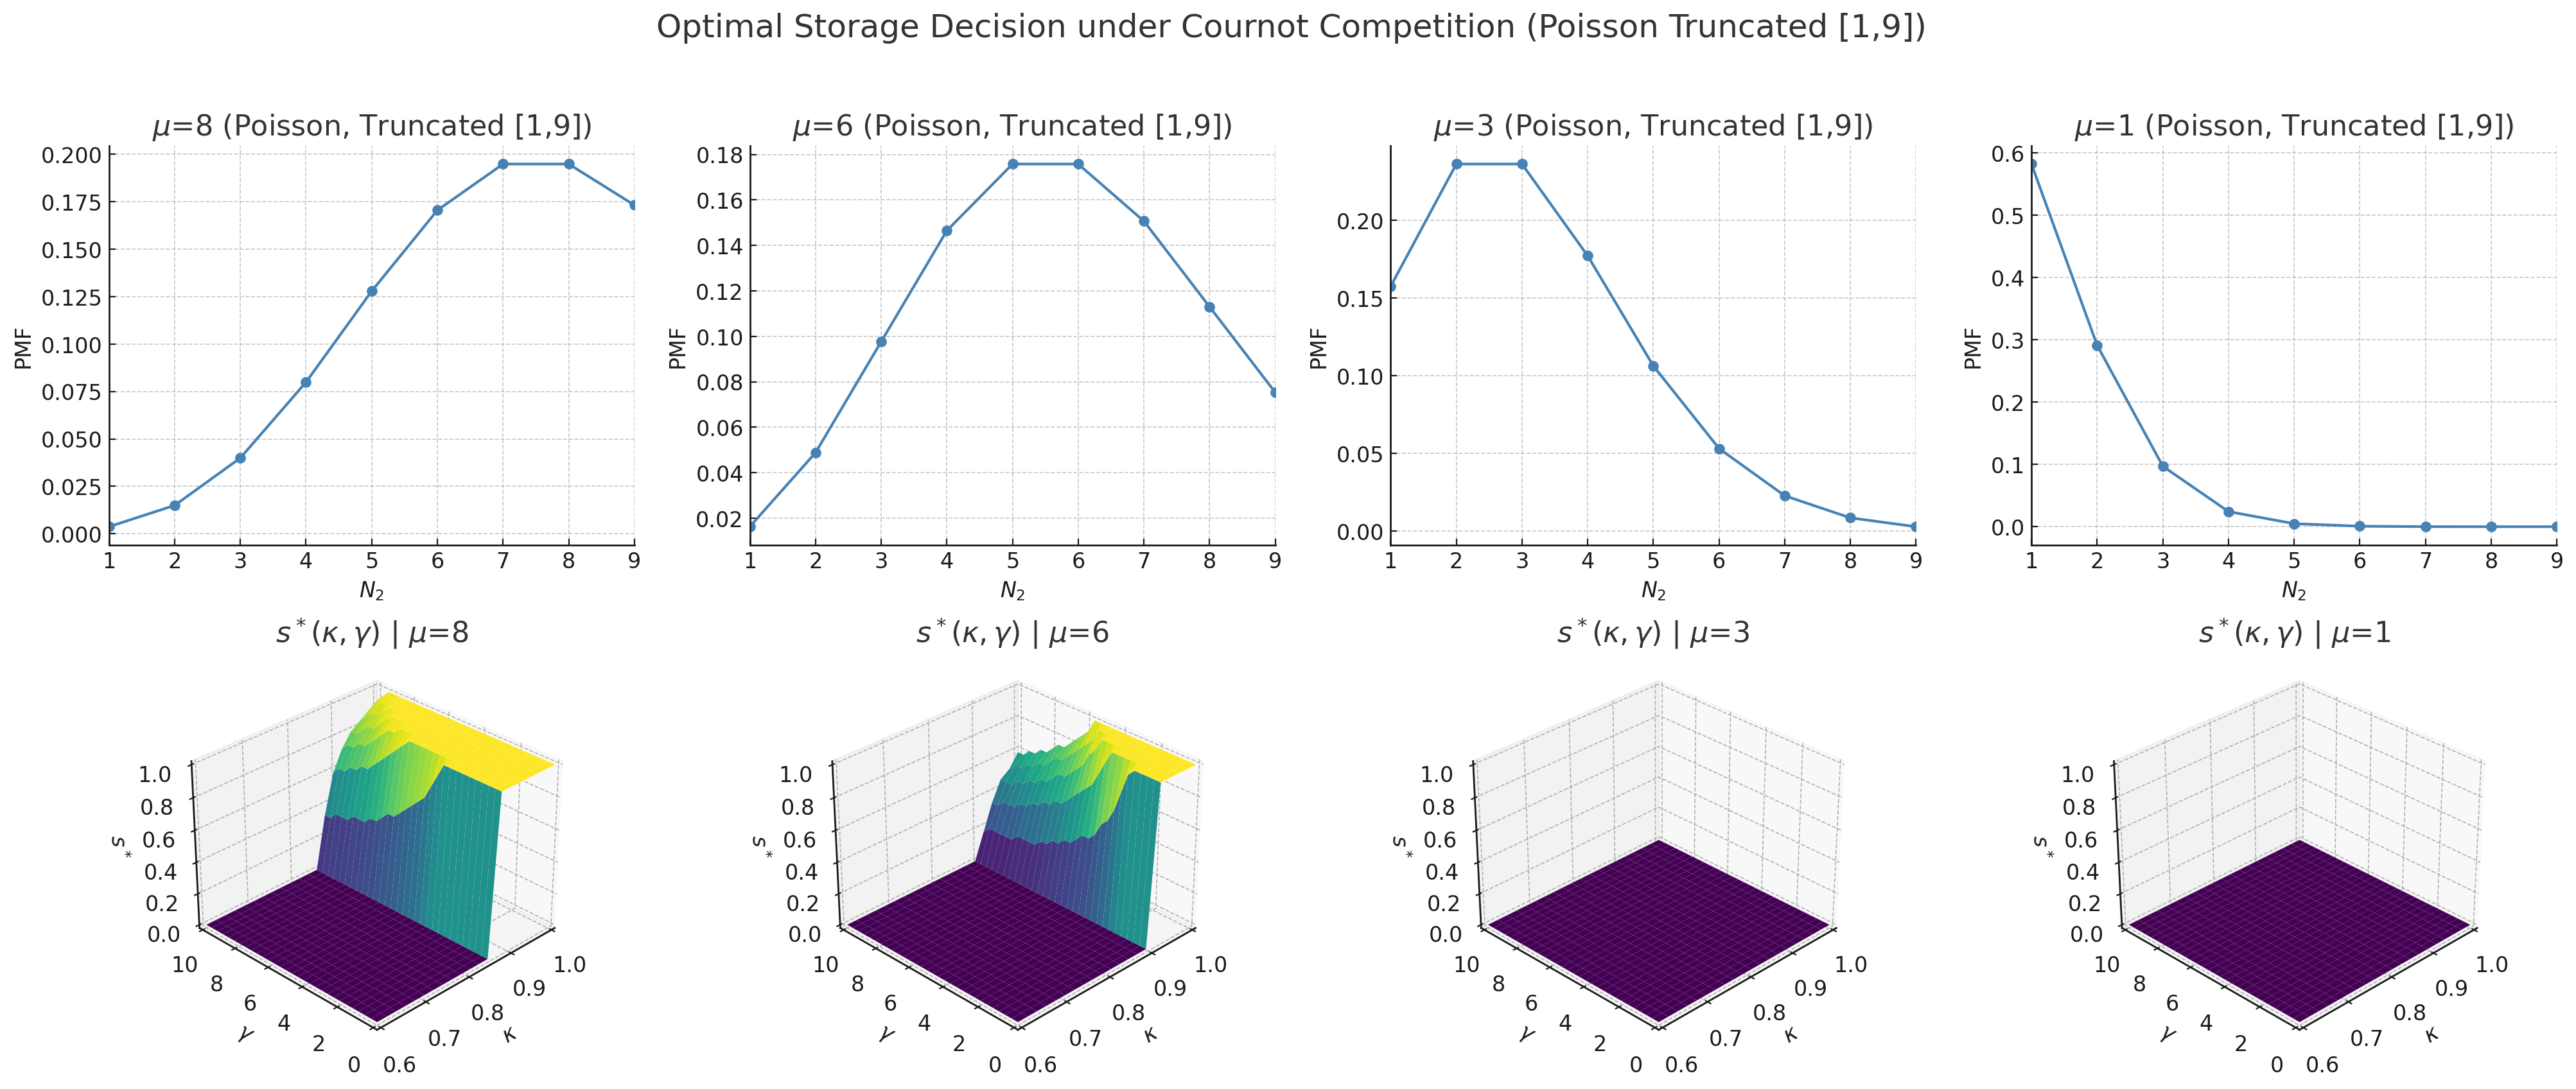
\includegraphics[width=\textwidth, keepaspectratio=true]{model_figures/3D_cournot.png}
        \caption{Optimal Storage Share and PDF Visualizations under Four Poisson Distributions of $N_2$}
        \label{Fig: 3D Cournot}
    \end{subfigure}
    
    \vspace{10mm} % Reduced vertical gap between subfigures
    
    \begin{subfigure}{\textwidth}
        \centering
        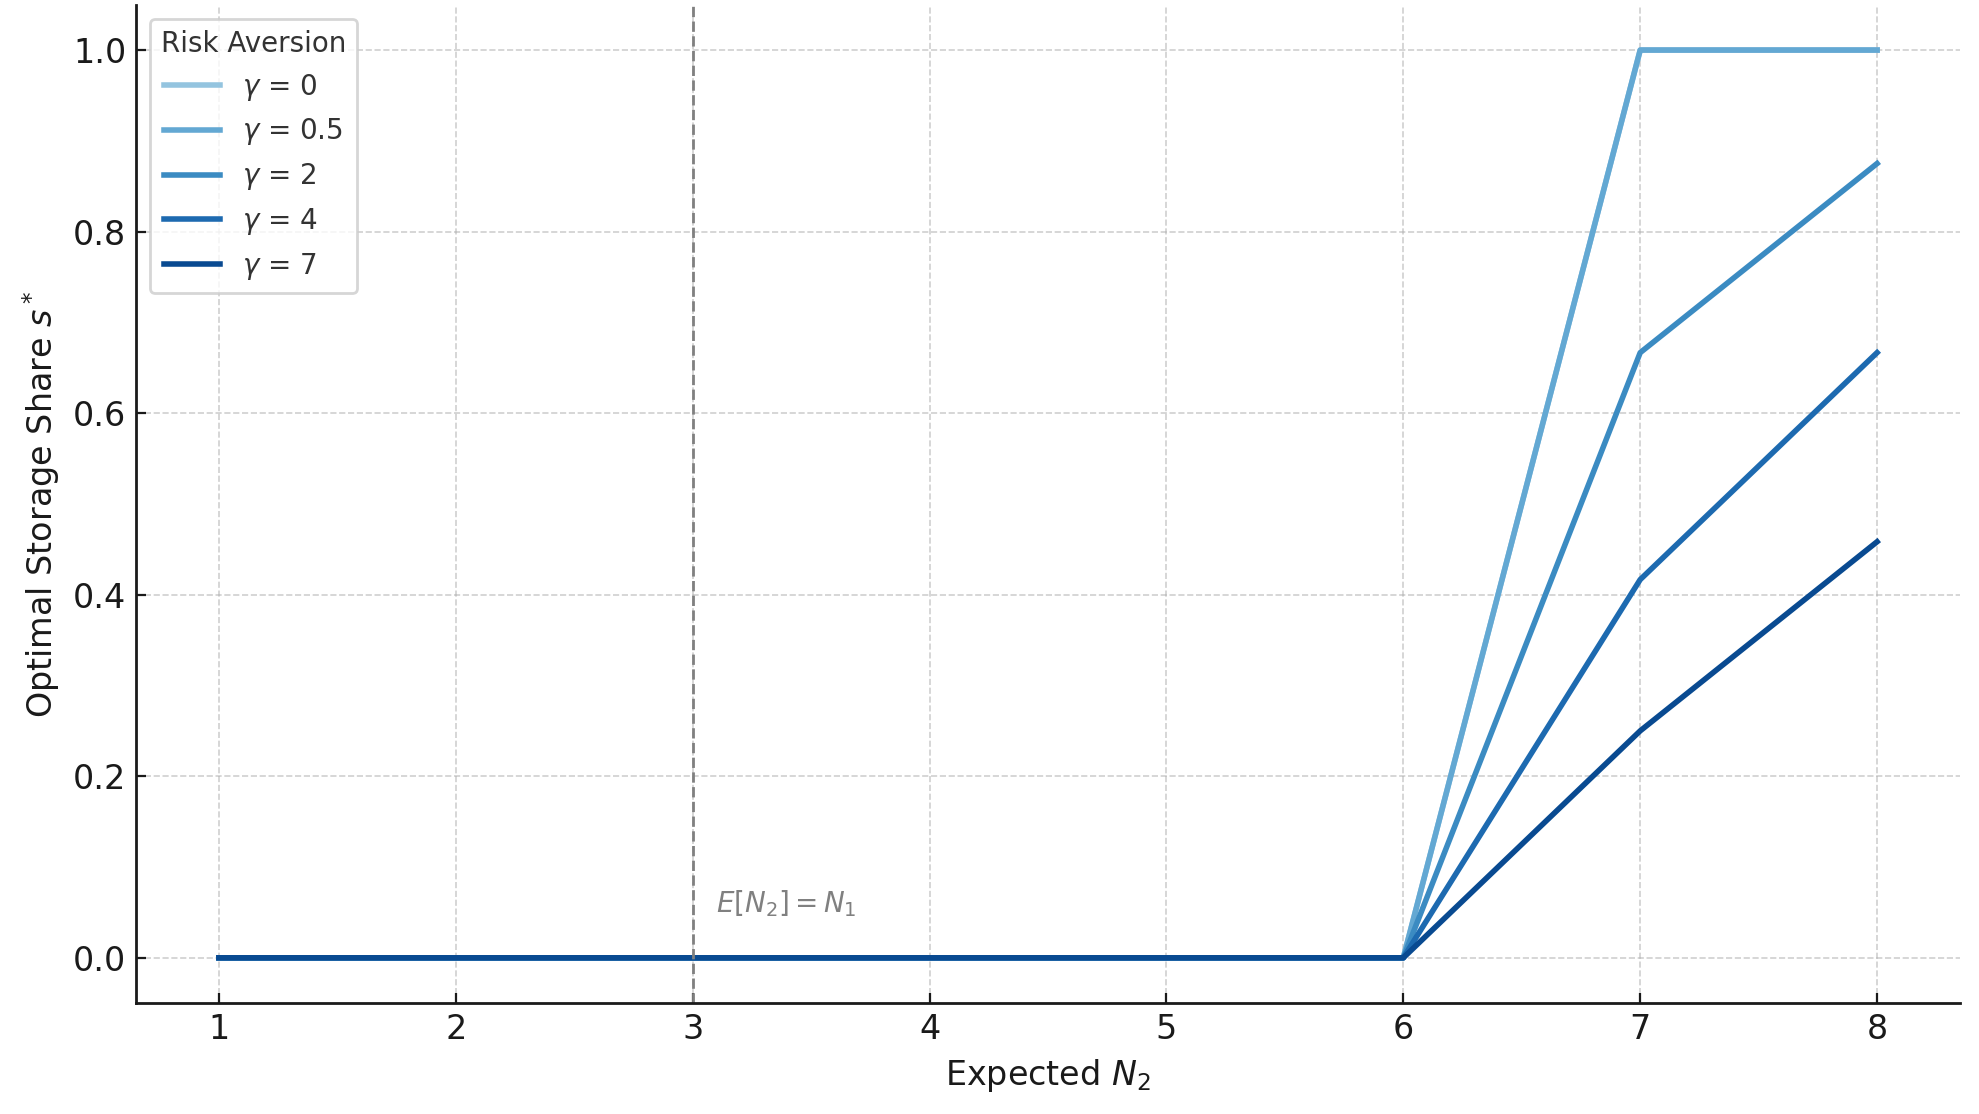
\includegraphics[width=\textwidth, keepaspectratio=true]{model_figures/buyer_count_sensitivity_cournot.png}
        \caption{Sensitivity to Expected Second-Period Buyer Presence ($\kappa=0.9$)}
        \label{Fig: Cournot sensitivity}
    \end{subfigure}

    \caption{Numerical Analysis under Cournot Competition}
\end{figure}



Figure~\ref{Fig: Cournot sensitivity} presents a three-panel sensitivity analysis of farmers' optimal storage share $s^*$ under Cournot competition when the second-period number of buyers follows a truncated Poisson distribution on $[0,9]$. The horizontal axis in each panel reports the expected value of $N_2$, and the vertical axis shows the corresponding optimal storage share. Each curve traces $s^*$ for a different level of risk aversion $\gamma \in \{0,0.5,2,4,7\}$, with darker shades of blue indicating higher $\gamma$. A vertical dashed line marks the benchmark case where the expected number of second-period buyers equals the observed first-period value, $\mathbb{E}[N_2]=N_1=3$. The three panels vary the assumed reservation price floor, $p_{\mathrm{reserve}} \in \{0.10,0.25,0.40\}$, which represents the outside option available if no standard buyers are present. This design allows direct comparison of how the outside option shifts storage incentives across risk preferences and market competitive scenarios.

Introducing a reservation price $p_{\text{reserve}}$ shifts the whole schedule upward in a economically intuitive way. A better fallback (from $0.10$ to $0.25$ to $0.40$) weakly lowers the threshold $\mathbb{E}[N_2]$ at which storage becomes attractive and increases $s^*$ at any given $\mathbb{E}[N_2]$-with the effect most pronounced for high $\gamma$, because the floor insures the downside of thin buyer markets. In short: more expected buyers and a stronger outside option both raise the optimal storage share, while greater risk aversion tempers that response.

On any particular curve plot in Figure~\ref{Fig: Cournot sensitivity}, increases in the expected second-period buyer count improve the attractiveness of storage. However, this does not always translate into a smooth rise in $s^*$: over a wide range of values for $N$, especially under high risk aversion, the optimal storage share remains at zero. Only once market prospects become sufficiently favorable does $s^*$ begin to increase, with less risk-averse farmers responding more readily to such improvements.


A key insight is that even under relatively favorable conditions-such as a low composite storage cost ($\kappa = 0.9$) and a moderately competitive harvest market ($N_1 = 3$)-storage becomes an attractive option only when farmers anticipate a substantially more buyer-presence market in the second period. Specifically, storage is only worthwhile when the expected number of buyers in period 2 reaches or exceeds 6, implying an expected price increase from $p_1 = \frac{3}{4} = 0.75$ to $p_2 = \frac{6}{7} \approx 0.857$. This 10.7 percentage point gain is sufficient to offset the 10\% effective loss due to storage inefficiency.


This result reflects the concave nature of the price function $p(N) = \tfrac{N}{N+1}$: as $N$ increases beyond 3, marginal improvements in price diminish. Therefore, even risk-neutral farmers require a strongly optimistic expectation of increased buyer presence to justify intertemporal arbitrage through storage. 

By contrast, when $N_1$ is very small (e.g., 1 or 2), the incremental price gains from attracting just one or two additional traders are much larger. For instance, moving from $N_1=1$ to $N_2=2$ raises the farm-gate price from $p_1=\tfrac{1}{2}=0.50$ to $p_2=\tfrac{2}{3}\approx 0.67$, while moving from $N_1=2$ to $N_2=3$ increases it further to $p_2=\tfrac{3}{4}=0.75$. Such discrete jumps can be large enough to incentivize storage. Thus, the stark threshold effect documented above is most relevant when the harvest market already exhibits moderate competition.





%----------------------------------------------------%
%----------------------------------------------------%


\section{Further Extensions}

\subsection{Other Models of Risk Preference}
\noindent According to \cite{o2018modeling}, ``Real-world risk aversion is clearly not as straightforward as expected utility suggests. Additional sources of risk aversion (or risk-seeking) need to be used instead of, or in conjunction with, diminishing marginal utility of wealth.'' Individuals assess options involving both gains and losses, the ``kink'' in the value function between losses and gains induces risk aversion. Therefore, future researchers may extend my model by exploring the Loss Aversion models \citep{kahneman1979prospect}, in addition to the expected utility theorem. The approach developed by \cite{kHoszegi2006model, kHoszegi2007reference, kHoszegi2009reference} in addressing loss aversion with an endogenous reference point aims to mitigate this degree of freedom by asserting that the reference point is entirely determined by one's expectations about outcomes. Empirical work also highlights the relevance of these alternative frameworks: for instance, \cite{liu2013risk} show that Chinese Bt cotton farmers’ pesticide use is systematically related to their risk and loss aversion, with more risk-averse farmers applying greater quantities of pesticides and more loss-averse farmers applying less. Despite this evidence, there has been limited progress in adapting alternative models to dynamic settings, with a notable exception of \cite{kHoszegi2009reference}, who define loss aversion concerning changes in beliefs regarding both current and future consumption.



\subsection{Collective-Action Dilemma: The Storage ``Treadmill''}
\noindent Field observations suggest a collective-action dilemma surrounding storage adoption. As more farmers in a village adopt storage, middlemen may redirect procurement efforts to neighboring villages with less storage penetration, where farmers face weaker bargaining positions. This strategic shift reduces buyer competition at harvest in the original village, particularly disadvantaging farmers without storage. Consequently, farmers who have not adopted storage face mounting pressure to invest, not necessarily for higher profits, but to avoid worsening terms of trade. 

This dynamic mirrors the classic ``technology treadmill'' described by Cochrane \citep{cochrane1958farm, levins1996treadmill}. It describes how technological progress in agriculture often fails to generate lasting gains for farmers. Early adopters of a new technology temporarily benefit from lower costs and higher profits, but as adoption spreads, aggregate supply expands and output prices fall due to the inelastic demand for food. These price declines erode the initial advantages, leaving non-adopters increasingly disadvantaged and eventually compelling them to adopt merely to maintain their previous income levels. In this way, technology adoption becomes a defensive necessity rather than a source of sustained profit. Future extensions of the model could incorporate this endogenous spillover, possibly via a parameter capturing buyer response to aggregate storage rates, highlighting how individually rational behavior may generate suboptimal collective outcomes.






\subsection{Non-linear Storage Cost}
\noindent Storage costs for farmers, defined as the sum of the actual cost of renting or operating storage space and the cost of deterioration, could be non-linear in many cases. For perishable goods like apples, the primary reason for convex storage costs is probably that spoilage and quality deterioration increase over time. Also, the operating costs of storage may not increase linearly with the volume of goods stored. Managing temperature and humidity conditions for larger quantities might require more sophisticated technology and energy consumption, leading to non-linear cost increases.

Supporting this notion, \cite{williams1989economic} demonstrates, through a quadratic form of total marketing costs, that farmers need to weigh the marginal revenue of later sales against the elevated costs incurred. This balance leads to a positive inventory, even without considering risk aversion. Instead of capturing the composite storage cost by a discounting factor, a well-designed mathematical model would allow other forms of storage costs, therefore, may give us other relevant real-world policy implications.


\section{Policy Implications}
\noindent
Whether in developing or advanced economies, policymakers care deeply about farm incomes. A common response has been direct interventions, such as minimum support prices or income transfers, that boost incomes but often at the cost of market distortions, fiscal burden, and misallocation of resources. The model here suggests an alternative emphasis: improve the environment in which farmers make intertemporal selling decisions. Three margins emerge from the analysis, competition, storage efficiency, and risk aversion, each capable of lifting expected incomes without direct price manipulation.



\subsection{Enhancing Competition among Buyers}

\textbf{Mechanism.} When competition among buyers is weak at harvest, farmers face low farm-gate prices. In the model this is captured by a high $\theta_1$, which depresses the immediate return to selling. Storage provides farmers with the option value of waiting, and its payoff rises if competition is expected to be stronger in the future, i.e.\ when the mean of $\theta_2$ falls and the second-period price distribution shifts upward. In this way, stronger future competition amplifies the benefits of storage by improving the relative return to waiting rather than selling at harvest.

\textbf{Quantitative illustration ($\delta=1$, $\kappa=0.9$, $\text{Var}(\theta_2)=0.02$):}
\begin{itemize}
  \item Suppose $\theta_1=0.5$ (harvest price $p_1=0.667$) and beliefs about buyer power shift from $\mu=0.37$ (weaker future competition) to $\mu=0.32$ (stronger future competition). Risk-neutral and risk-averse ($\gamma=2$) farmers both switch from \emph{no storage} to \emph{full storage}. Expected income rises from $0.667$ to $0.690$, a gain of $+\;0.023$.
\end{itemize}

\textbf{Policy interpretation.} When policies succeed in enhancing buyer competition at harvest, the immediate farm-gate price $p_1$ rises, thereby improving farmer welfare unconditionally. In practice, however, such interventions may not always produce an immediate effect at the start of the marketing season. The model indicates that as long as buyer competition improves at any point during the marketing period, farmers can still possibly benefit through storage. Relevant policy instruments include stricter antitrust enforcement to deter collusion, lowering entry barriers for new traders, and investments in digital trading platforms or logistics infrastructure that expand farmers’ access to alternative buyers throughout the season.






\subsection{Subsidizing Storage and Technology Adoption}

\textbf{Mechanism.} The model shows that improving storage efficiency---captured by a higher $\kappa$---raises the net return from delaying sales. In practical terms, farmers retain more value from what they store, making the option to wait more attractive. This effect is particularly strong when market conditions are finely balanced, because even a modest improvement in storage efficiency can shift farmers from selling immediately to storing their entire harvest.

\textbf{Quantitative illustration (fix $\theta_1=0.5 \Rightarrow p_1=0.667$, $\delta=1$, $\text{Var}(\theta_2)=0.02$; raise $\kappa$ by 10\% from $0.90 \to 0.99$):}
\begin{itemize}
  \item At $\mu=0.33$, risk-neutral farmers already store fully, but expected income still rises markedly from $0.684$ to $0.752$ ($+\;0.068$).
  \item At $\mu=0.35$, risk-neutral farmers continue to store fully, while moderately risk-averse farmers ($\gamma=2$) increase storage from 50\% to 100\%; their expected income rises from $0.670$ to $0.741$ ($+\;0.071$).
  \item At $\mu=0.37$, right at the margin, both risk-neutral and risk-averse farmers switch from no storage to full storage, with expected income increasing from $0.667$ to $0.730$ ($+\;0.063$).
\end{itemize}

\textbf{Policy interpretation.} A 10\% increase in storage efficiency yields substantial income gains---on the order of 6--7 percentage points---and can induce dramatic behavioral shifts in storage, especially near the decision boundary. These results suggest that policies which subsidize storage or promote better technologies (e.g., air-controlled cold storage, or improved post-harvest handling) can deliver sizable welfare benefits without distorting market prices. Even though previous studies like \cite{nindi2024incentive} have demonstrated that combining storage technology that is localized and flexible can lead to better post-harvest outcomes for smallholder farmers, our model points out another role of storage subsidy: unlike direct price supports, which are costly and often inefficient, improving $\kappa$ raises returns across the board and strengthens farmers' ability to capture intertemporal gains from time-varying oligopsonistic power change alone.  






\subsection{Reducing Effective Risk Aversion via Financial Deepening}

\textbf{Mechanism.} While intrinsic risk preferences are relatively stable, \emph{effective} risk aversion declines as farmers gain financial security through liquidity, insurance, and wealth accumulation. A lower coefficient of relative risk aversion ($\gamma$) shifts behavior toward the risk-neutral benchmark, with the largest effects concentrated in the region where storage is only marginally profitable in expectation.


\begin{figure}[ht!]
    \centering
    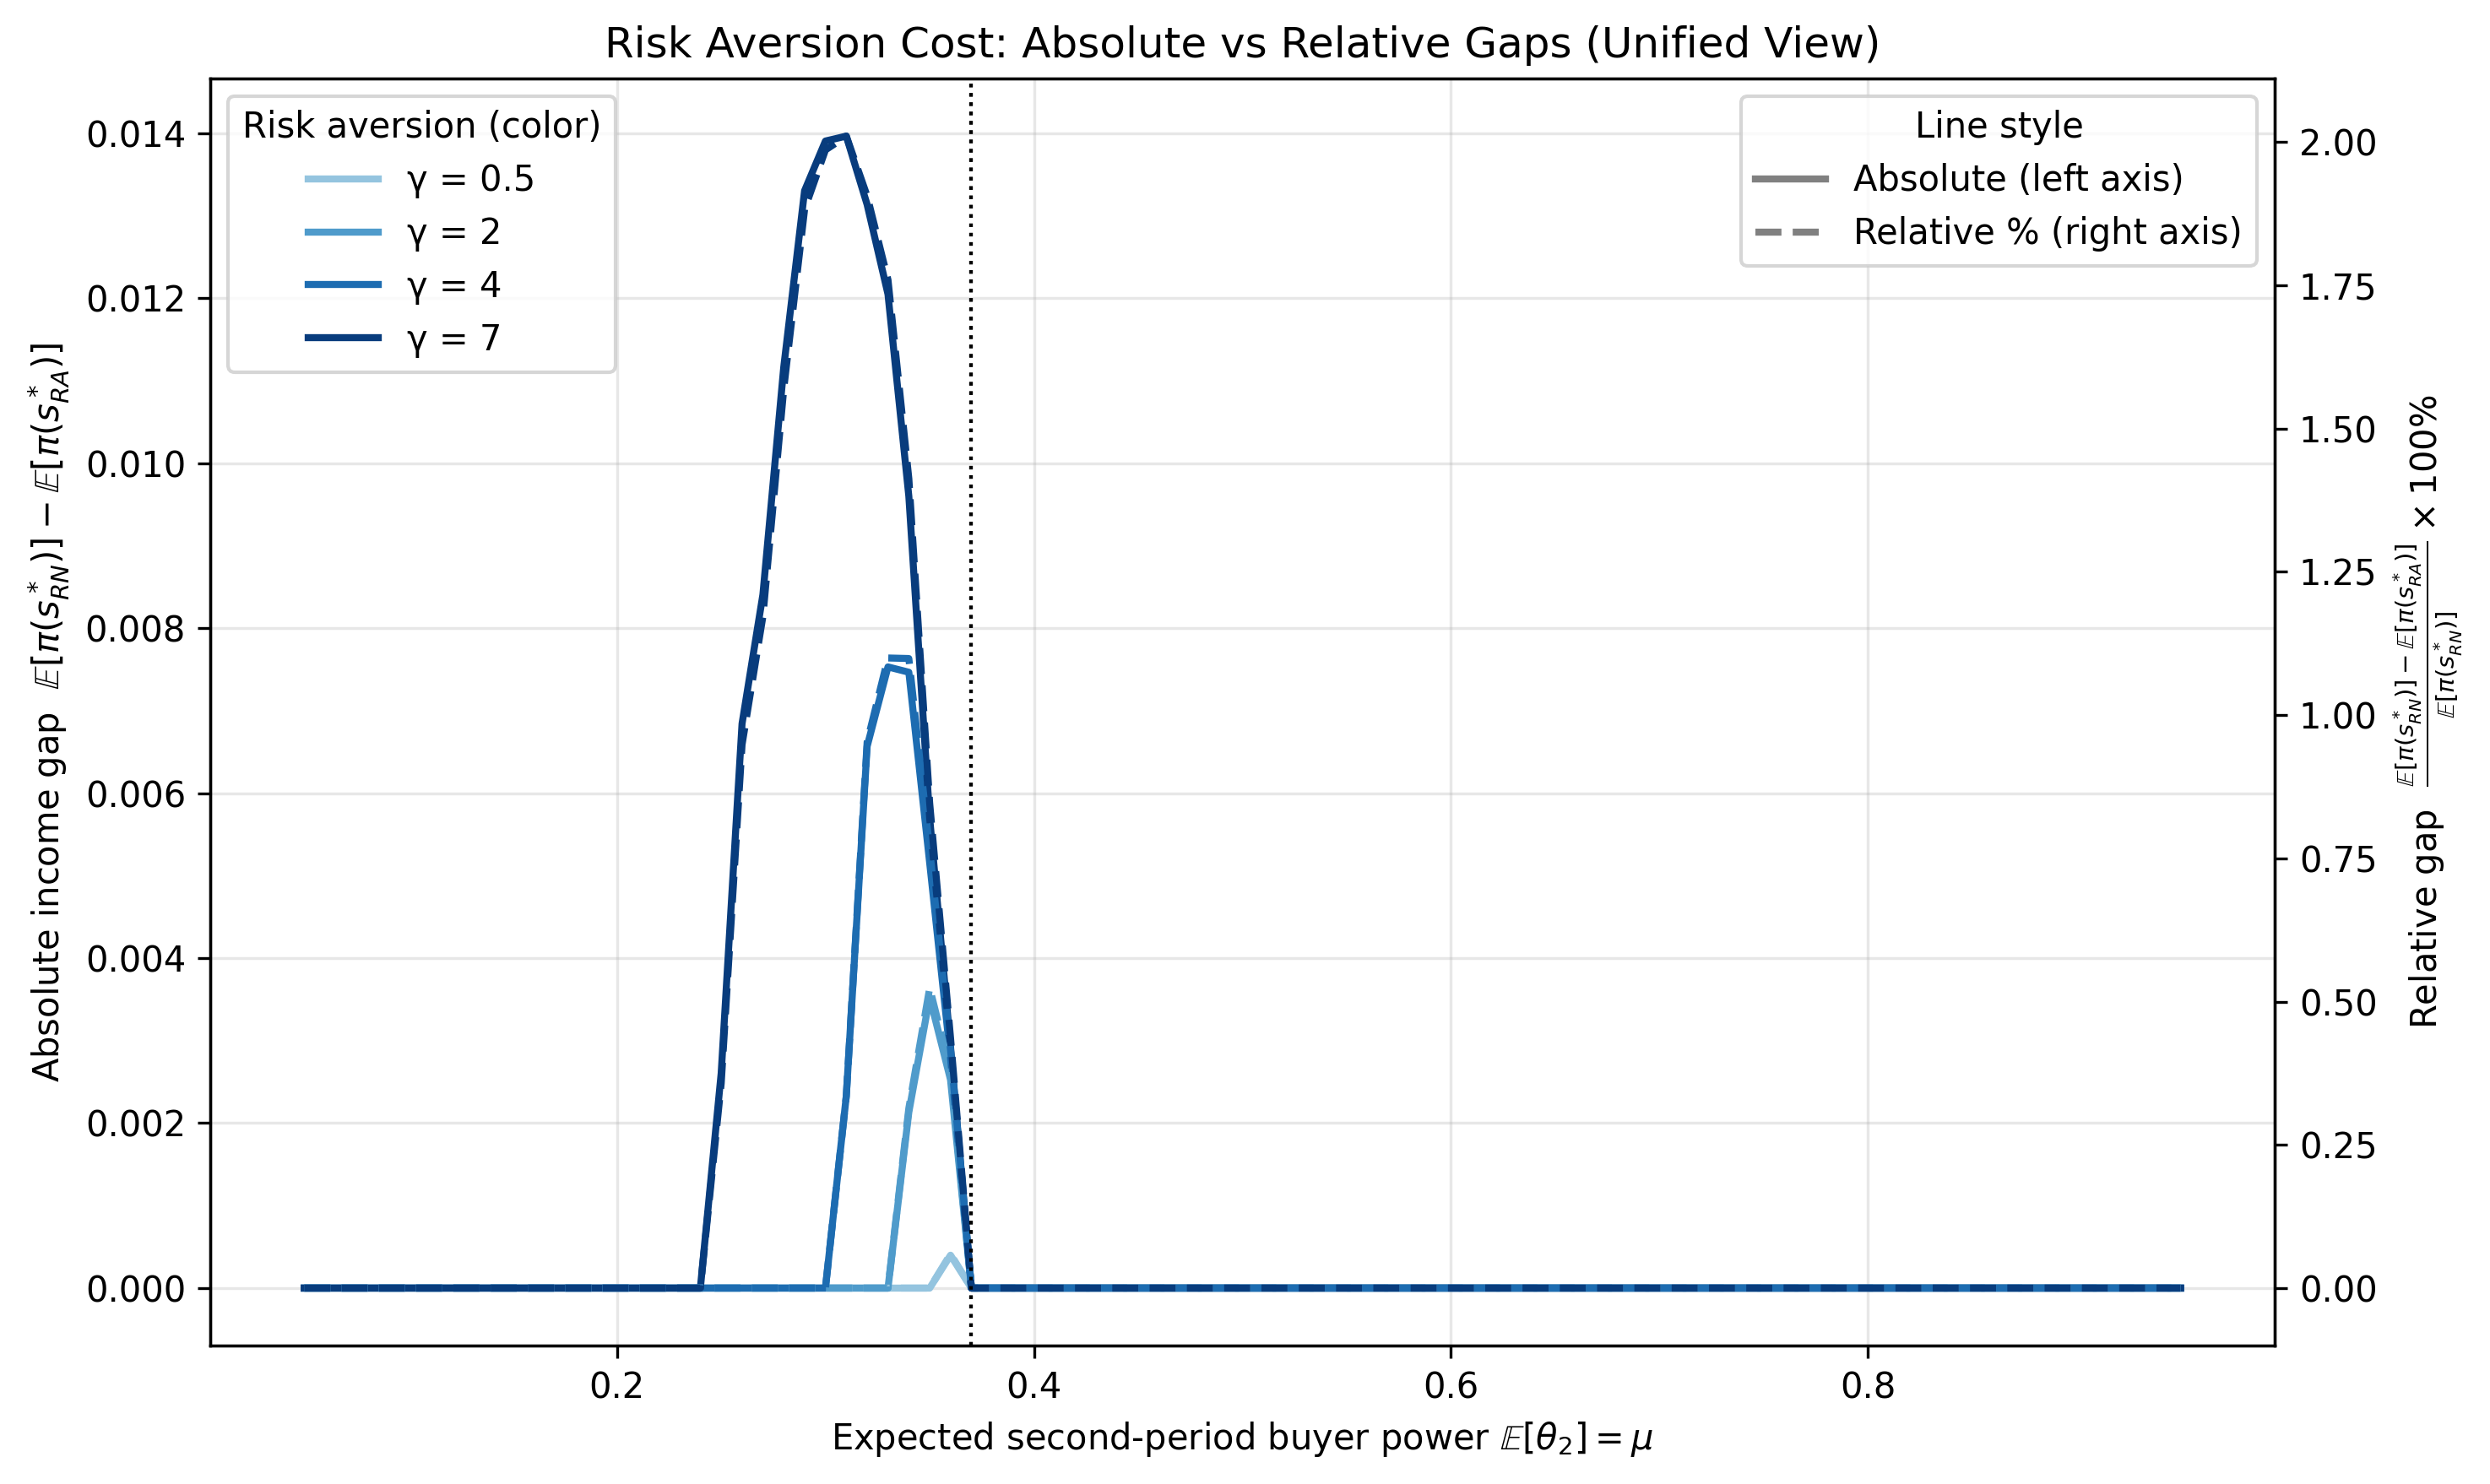
\includegraphics[width=0.85\textwidth]{model_figures/income_gap_vs_mu_(unified).png}
    \caption{Absolute and relative expected income losses from risk aversion. 
    Solid lines show the absolute gap $\mathbb{E}[\pi(s^*_{RN})]-\mathbb{E}[\pi(s^*_{RA})]$ (left axis). 
    Dashed lines show the same gap as a percentage of the risk-neutral benchmark (right axis). 
    Colors indicate the degree of risk aversion ($\gamma$). 
    The vertical dotted line marks the risk-neutral switching threshold $\mu^\star$ where storage ceases to be profitable.}
    \label{fig:unified_gap_plot}
\end{figure}


\textbf{Quantitative illustration:} The Simulation results from the baseline model in Figure~\ref{fig:unified_gap_plot} show that absolute income losses from risk aversion peak at roughly 0.02--0.03 in normalized units, while the relative gap reaches about 2 percent of expected income under strong risk aversion ($\gamma=7$) and falls below 1 percent for moderate values ($\gamma=2$ to $4$). These effects vanish when storage is clearly profitable or clearly unprofitable, underscoring that the ``cost of risk aversion'' is concentrated exactly at the margin where storage incentives are fragile.

\textbf{Policy Interpretation.} The income effect from lowering risk aversion is modest in size but targeted: it recovers the ``money left on the table'' precisely where risk aversion binds most. Instruments that ease liquidity risk (warehouse-receipt finance, seasonal credit lines), transfer income across states (crop insurance), or smooth consumption (safety nets) can move farmers measurably closer to the risk-neutral storage decision. Even modest financial deepening---for example, reducing effective $\gamma$ from 7 to 2---eliminates more than half of the small but systematic income gap in this calibration.










\section{Welfare Gains from Storage Subsidy}
\noindent
A central implication of the storage model is that policies which reduce the effective cost of storage can generate direct income and welfare gains. To formalize this insight, I extend the baseline framework by allowing both first- and second-period buyer power to be stochastic, drawn from a common distribution. In this environment, farmers’ incentives to store depend not only on realized prices but also on their heterogeneous attitudes toward risk and patience. I therefore construct a simulated “village” of farmers who are identical in production but vary in risk preferences, and analyze how shifts in the storage efficiency parameter $\kappa$---interpretable as reductions in physical losses or lower discounting---translate into higher expected incomes and certainty-equivalent welfare. This exercise highlights the development potential of storage as a strategy to reduce vulnerability while enhancing the long-run earnings capacity of smallholders.


Let's model the buyer power terms in both trading periods in our base model in Equation~\ref{eq:final objective} as random variables supported on $[0,1]$. Specifically, I assume $\theta_1$ and $\theta_2$ are i.i.d. draws from a Beta$(\alpha,\beta)$ distribution. For a given mean belief $\mu$ and variance $\sigma^2$, the Beta parameters are calibrated. By varying $\mu$ across $[0.05,0.95]$ with fixed variance $\sigma^2=0.02$, I can map a wide array of possible beliefs about the competitiveness of second-period markets.


The expectation over $\theta_2$ is evaluated using Gauss–Legendre quadrature. I compute quantile nodes from the Beta distribution and weight them appropriately to obtain accurate approximations to $\mathbb{E}[U(\pi(s;\theta_1,\theta_2))]$. To solve for the optimal storage share, I evaluate expected utility on a coarse grid of 33 points between 0 and 1, identify the best candidate, and then refine locally on a denser subgrid. To avoid recomputing this solution for every farmer and every simulated world, I precompute a lookup surface $s^{*}(\theta_1,\gamma;\kappa)$ over a 15-by-15 tensor grid in $\theta_1$ and $\gamma$, and then interpolate bilinearly during the simulation.

The simulation design proceeds in several layers. First, I construct a “village” of 100 farmers, each endowed with one unit of harvest. Heterogeneity arises solely from risk preferences: I draw coefficients of relative risk aversion $\gamma_i \sim U[0,10]$ and hold this population fixed across all counterfactuals. To assess distributional effects, I sort these farmers into deciles of the $\gamma$ distribution. Second, for each mean belief $\mu$ in the sweep, I simulate 280 season-worlds, each consisting of an independent draw of $(\theta_1,\theta_2)$ from the calibrated Beta distribution. To ensure comparability across policy regimes, I implement a “common-shocks” design: the same set of season-worlds is used to evaluate outcomes under each storage efficiency $\kappa$. This isolates the impact of policy from the stochasticity of draws.

For each farmer $i$ in each world $r$, the interpolated optimal storage share $s_i^{*(r)}$ is combined with the realized prices to yield income $\pi_i^{(r)}$. Averaging across worlds gives the farmer’s expected income $\bar{\pi}_i$ and expected utility $\bar U_i$. The latter is converted back into a certainty equivalent,
$$
\text{CE}_i = U^{-1}(\bar U_i),
$$
which represents the sure level of income yielding the same utility as the risky prospect. From these objects I compute the risk premium,
$$
\text{RP}_i = \bar \pi_i - \text{CE}_i,
$$
the wedge between expected income and its certainty equivalent. By aggregating across farmers, I obtain village-level means for income, certainty equivalent, and risk premium. By further breaking results out by decile of $\gamma$, I can characterize how risk preferences shape the incidence of storage policies.

This setup permits a natural decomposition of welfare effects from changes in storage efficiency. For any policy step that raises $\kappa$ from $\kappa_0$ to $\kappa_1$, the gain in certainty equivalent is
$$
\Delta \text{CE}_i = \underbrace{\Delta \bar \pi_i}_{\text{growth}} \;+\; \underbrace{\big(-\Delta \text{RP}_i\big)}_{\text{insurance}}.
$$
The first term captures the mechanical effect of higher efficiency on expected returns, while the second term captures the reduction in exposure to risk, which is especially valuable to highly risk-averse farmers. This decomposition, averaged across farmers or examined decile by decile, makes transparent the twin channels through which storage policy improves welfare.



\begin{figure}[ht!]
    \centering
    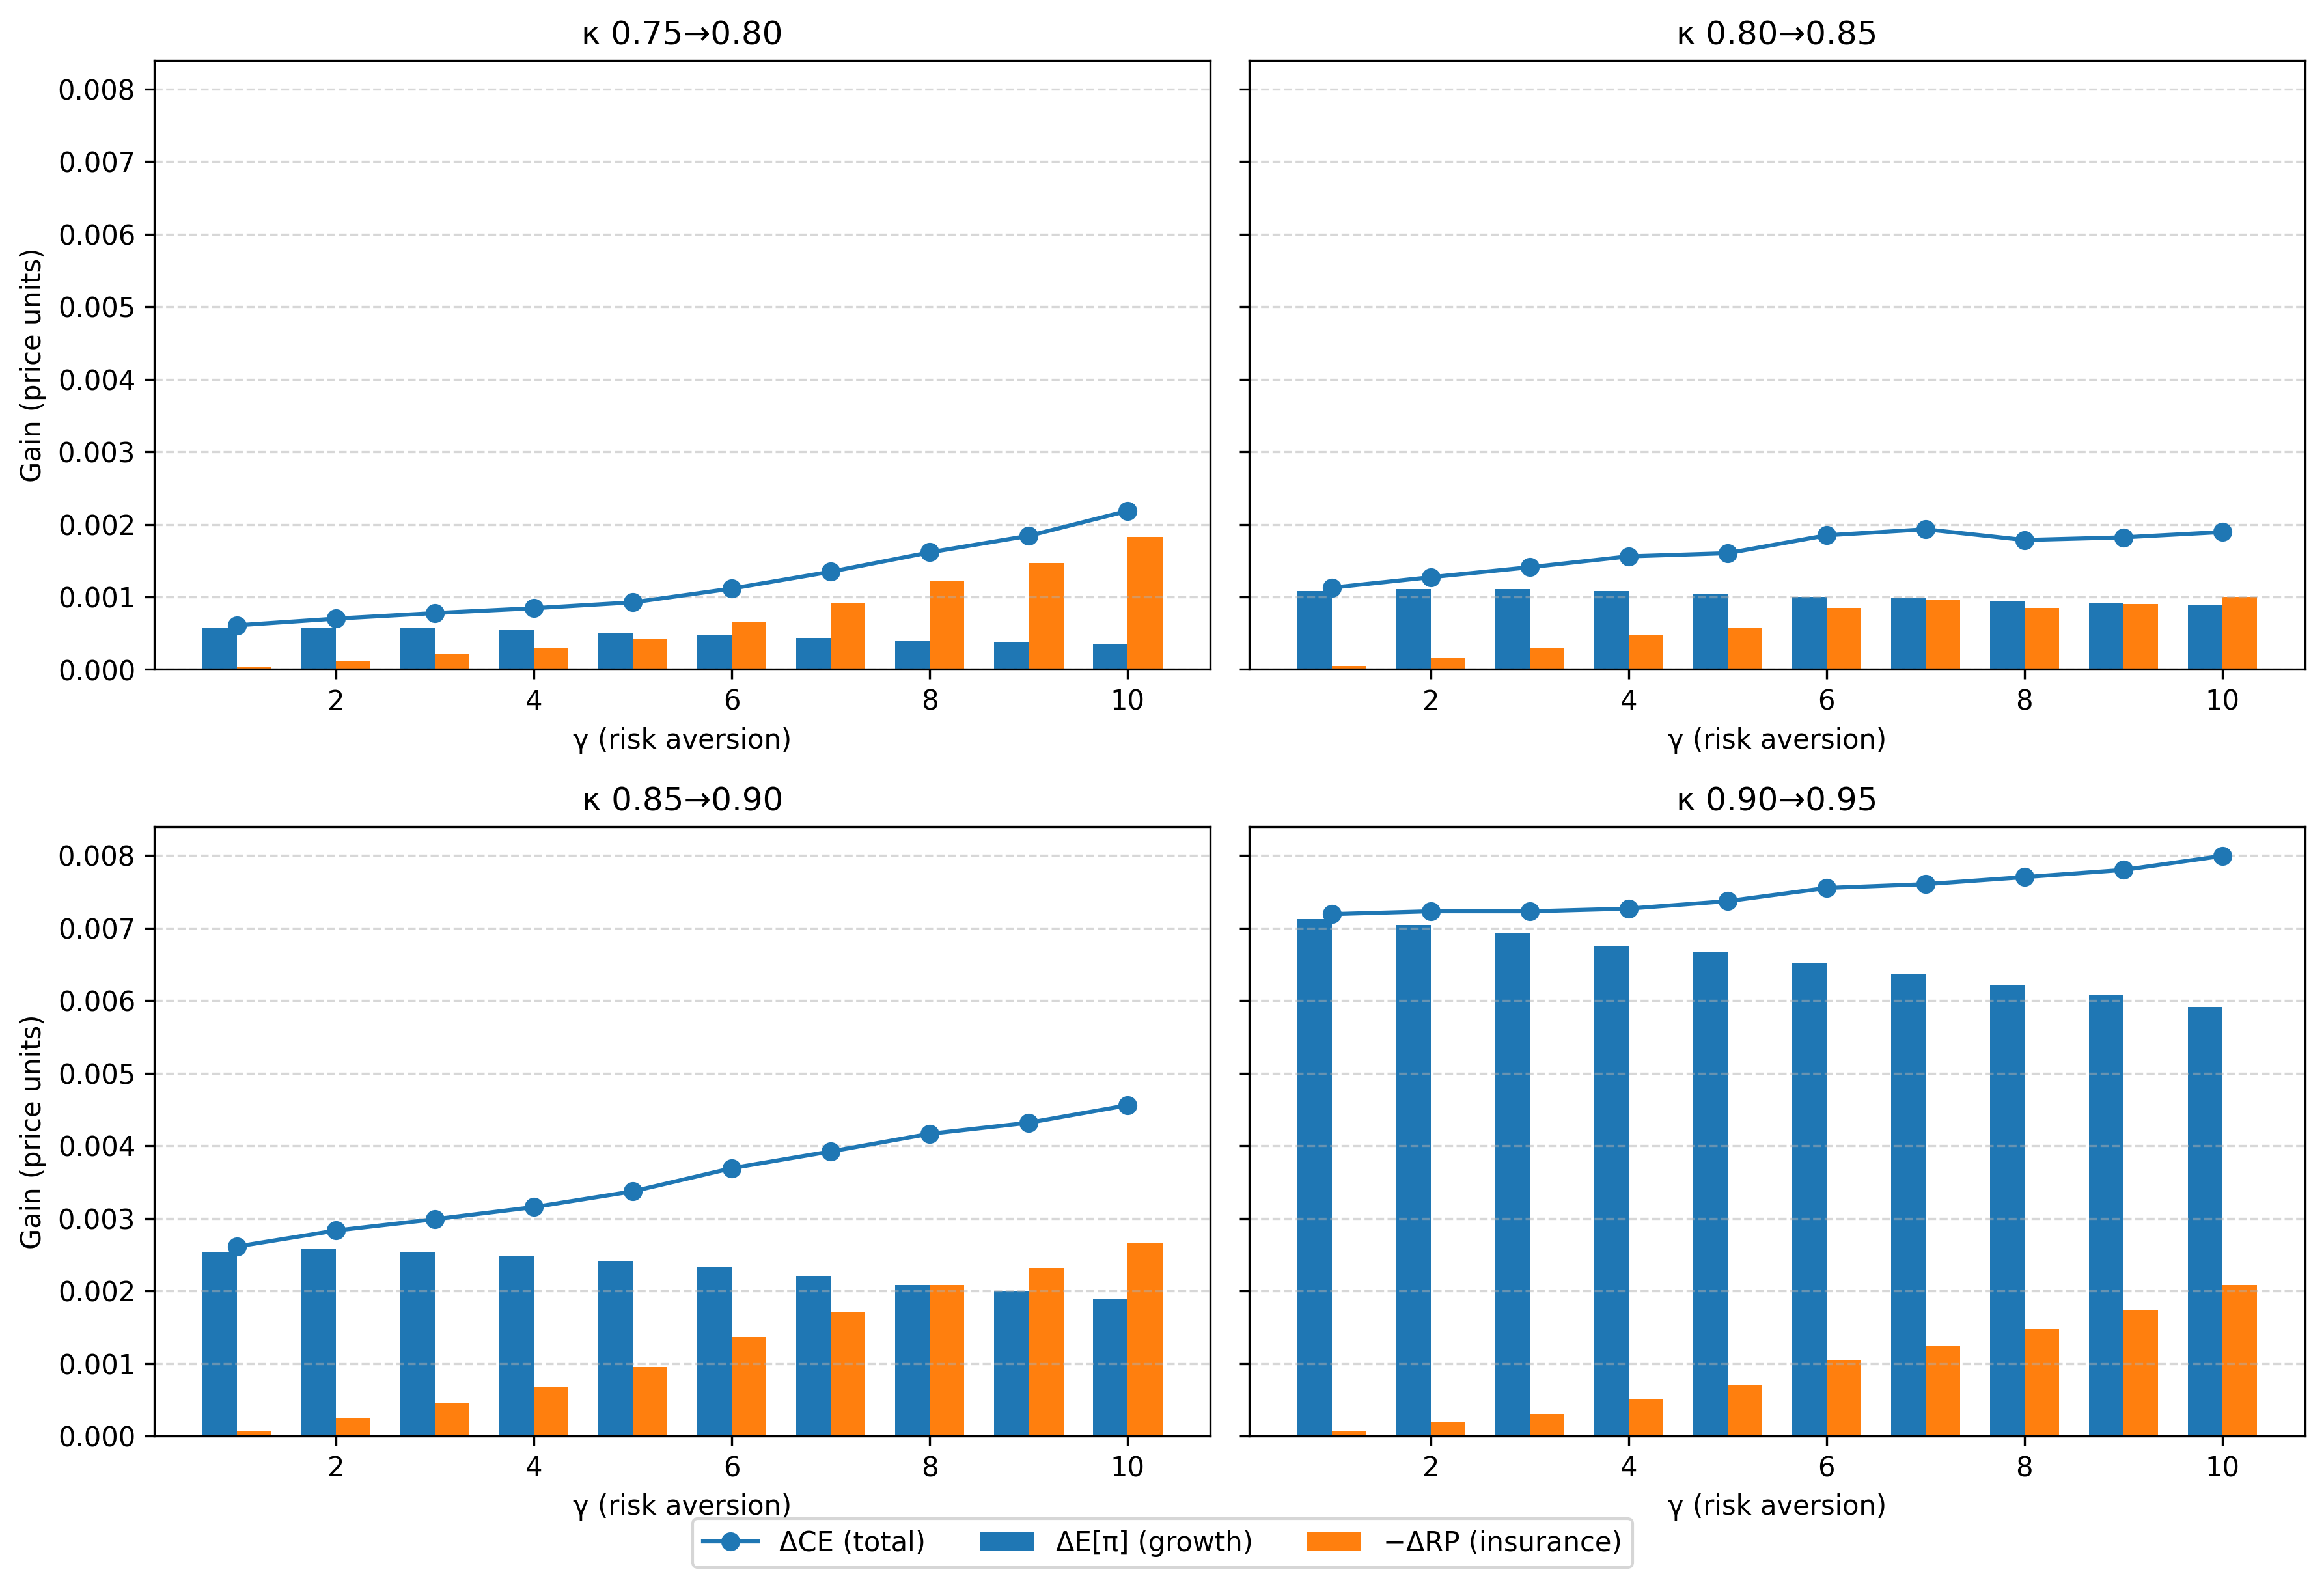
\includegraphics[width=\textwidth]{model_figures/storage_subsidy_gain_decomposition.png}
    \caption{Welfare Decomposition by Risk Aversion}
    \label{fig:storage_subsidy_gain_decomposition} 
    \begin{tablenotes}
    \footnotesize
    \item Note: Each panel shows a $\kappa$ contrast. Bars plot the growth component ($\Delta E[\pi]$) and the insurance component ($- \Delta RP$); the line plots total welfare ($\Delta CE$), which satisfies $\Delta CE \approx \Delta E[\pi] + (- \Delta RP)$. Higher $\kappa$ steps scale up both components, with insurance gains concentrated in higher $\gamma$-deciles.
    \end{tablenotes}
\end{figure}

Figure~\ref{fig:storage_subsidy_gain_decomposition} reports a 2×2 grid that shows this decomposition across the distribution of risk preferences. Each panel corresponds to one contrast in storage efficiency, $\kappa \in \{0.75\to0.80,\,0.80\to0.85,\,0.85\to0.90,\,0.90\to0.95\}$. Within a panel, the horizontal axis indexes risk-aversion deciles ($\gamma$-decile 1 = least risk-averse, 10 = most). For each decile we plot: (i) a bar for the change in expected income, $\Delta E[\pi]$ (``growth''), (ii) a bar for the insurance gain, $-\Delta RP$ (the reduction in risk premium, shown as a positive quantity), and (iii) a line for the total welfare effect, $\Delta CE$.

The layout delivers two comparative-statics at a glance. Across deciles within a panel, we read distributional incidence: where the $-\Delta RP$ bar grows with $\gamma$, the subsidy operates predominantly through the insurance channel, disproportionately benefiting more risk-averse farmers. Across panels, we track how the magnitude and composition of benefits evolve as $\kappa$ rises. Deeper storage subsidies usually shift the entire profile upward, with both bars and the $\Delta CE$ line moving higher across deciles, while the relative contributions of growth and insurance vary. Overall, the figure shows that storage subsidies generate meaningful welfare improvements through both channels, with insurance gains especially important for high-$\gamma$ farmers and aggregate benefits rising with the size of the $\kappa$ improvement.



\begin{figure}[ht!]
    \centering
    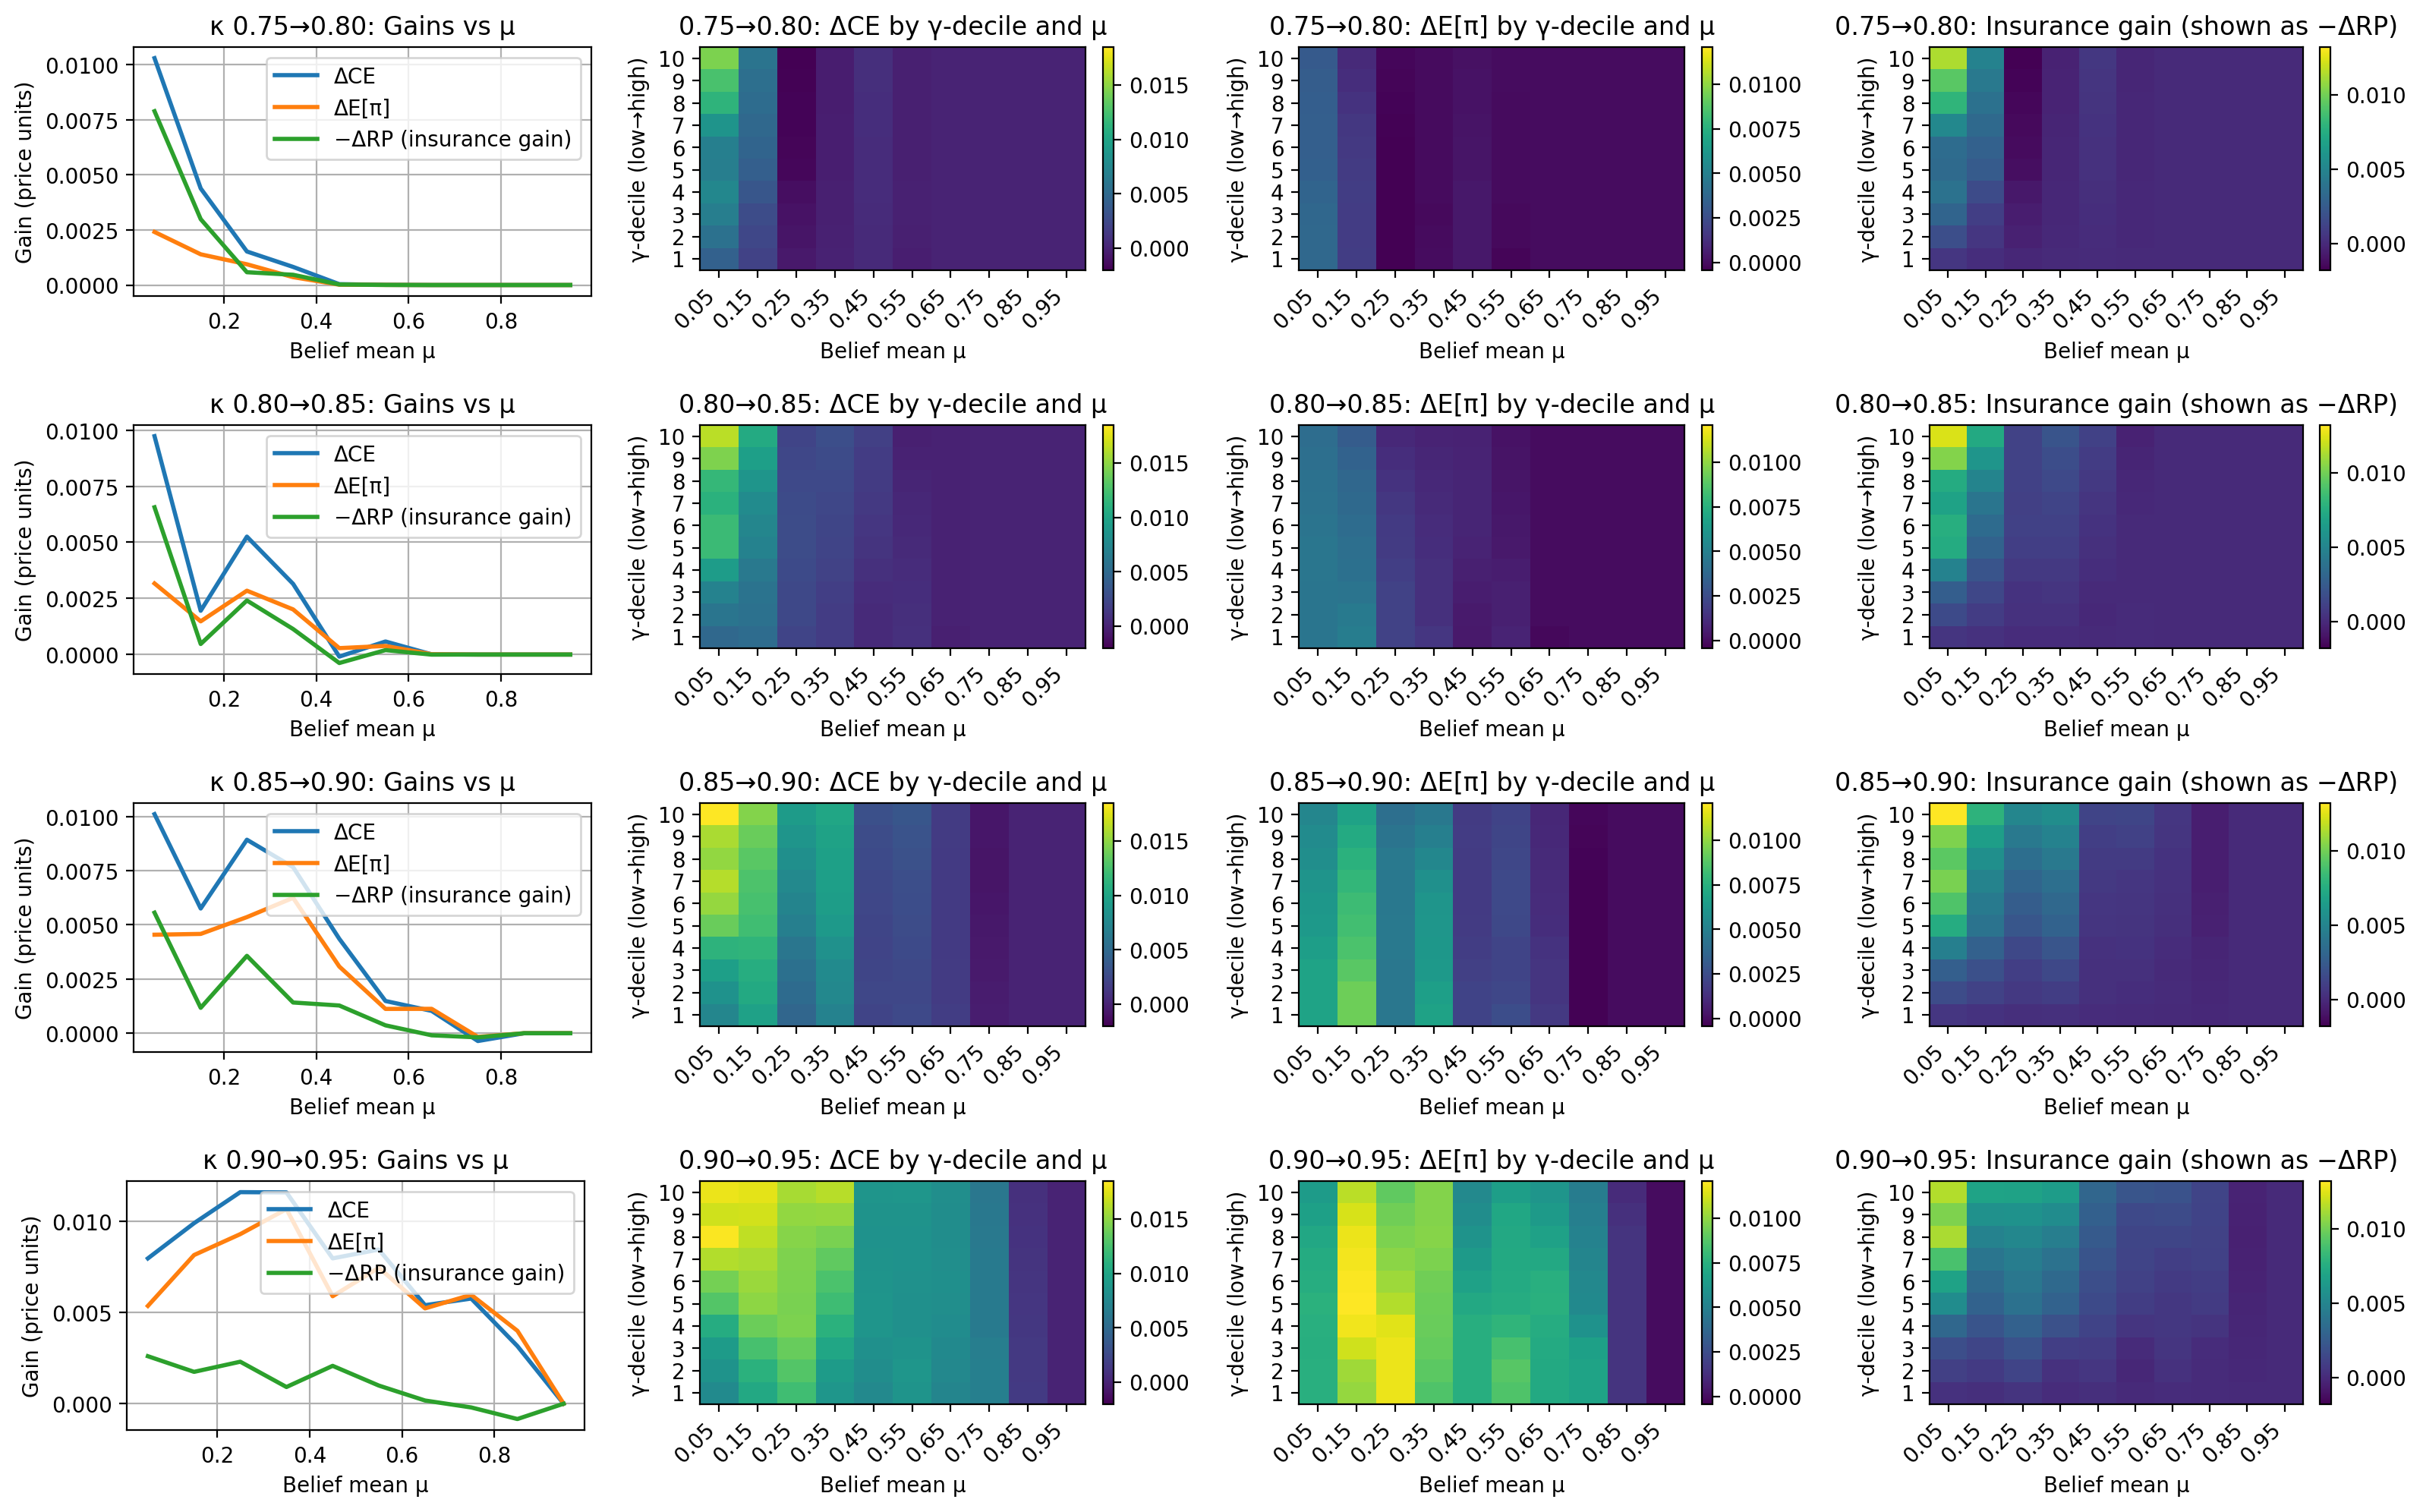
\includegraphics[width=\textwidth]{model_figures/storage_subsidy_gain_heatmap.png}
    \caption{Average and Distributional Gains from Incremental Storage Subsidies}
    \label{fig: storage_subsidy_gain_heatmap}
    \begin{tablenotes}
    \footnotesize
    \item Note: Each row shows one subsidy contrast. Line charts (first column) plot changes in expected income ($\Delta E[\pi]$), certainty equivalent ($\Delta CE$), and insurance gain ($-\Delta RP$) against belief mean $\mu$. Heatmaps (columns 2--4) decompose these effects across $\gamma$-deciles, highlighting that welfare improvements are strongest for more risk-averse farmers and grow with the size of the subsidy.
    \end{tablenotes}
\end{figure}


Figure~\ref{fig: storage_subsidy_gain_heatmap} presents a $4 \times 4$ panel that summarizes how incremental improvements in storage efficiency affect farmer welfare and income. Each row corresponds to one subsidy contrast ($\kappa: 0.75 \rightarrow 0.80$, $0.80 \rightarrow 0.85$, $0.85 \rightarrow 0.90$, and $0.90 \rightarrow 0.95$), designed to mimic modest policy interventions. The first column shows line charts of three gain measures as a function of farmers’ beliefs about buyer competitiveness ($\mu$): the expected income effect ($\Delta E[\pi]$), welfare effect ($\Delta CE$), and insurance gain ($-\Delta RP$). Whereas $\Delta E[\pi]$ captures direct profit improvements and $\Delta CE$ also reflects reduced risk exposure. The remaining columns provide heatmaps that decompose these effects across deciles of risk aversion ($\gamma$), with lighter colors signifying greater gains. These reveal whether benefits are uniform across beliefs and preferences or concentrated among more risk-averse farmers and high-$\mu$ environments.

Across subsidy contrasts, welfare improvements are modest when $\kappa$ rises from $0.75$ to $0.80$, but intensify as $\kappa$ approaches $0.95$. In all cases, risk-averse farmers capture disproportionate benefits from the insurance channel, while risk-neutral farmers mainly gain from higher expected profits. The magnitude of gains is further shaped by beliefs on buyer power. 





\section{Conclusion}

\noindent This chapter develops a conceptual framework to analyze farmers' storage behavior under buyer market power. Storage adoption creates an inter-temporal arbitrage margin that allows farmers to shift sales across periods, thereby mitigating the effects of oligopsony at harvest and enhancing their bargaining position. The model shows that even absent shifts in aggregate demand or supply, temporal variation in buyer competition alone can make storage a valuable marketing tool.

The model provides a theoretical basis for small-scale farmers' storage and marketing choices. It focuses on farmers' intra-seasonal strategies and the storing-decision process, where farmers observe farm-gate prices and market structure at harvest and decide whether to immediately sell some, all, or none of their crops. When farmers have insufficient bargaining power at a single point in time, the adoption of storage at lower storage costs would give them inter-temporal arbitrage opportunities.

Although motivated by the fresh-apple industry, the model's logic applies broadly across perishable commodities. Storage and inventory play a central role in agricultural marketing systems, not only smoothing demand-driven price fluctuations but also reshaping the strategic interaction between growers and buyers. Framing storage as a tool to navigate imperfect competition thus extends beyond post-harvest logistics to the core of market efficiency and farmer welfare.

Policy implications follow directly from the analysis. First, lowering storage costs through subsidies, credit, or investment in modern facilities expands the set of circumstances under which farmers can profitably store and arbitrage across periods. Second, strengthening competition among buyers, via enforcement of antitrust rules, lower entry barriers for new buyers, or improved transparency in local markets, raises the effective price level and reduces the rents extracted by middlemen. Third, reducing the effective bite of risk aversion, through crop insurance, safety nets, or access to seasonal finance, encourages farmers to undertake storage when it is profitable in expectation but risky. Together these instruments highlight a policy strategy that does not rely on direct price support or costly procurement programs, but instead empowers farmers to use inter-temporal arbitrage to raise incomes and improve efficiency along the supply chain.






% %---------------------------%
% \newpage
% \section{Memo: A Difficult Tradeoff between Two Utility Aggregation Approaches}
% \noindent As I finalize revisions on the current model, I identify a major conceptual drawback: the optimal storage share becomes increasing in the farmer's degree of risk aversion when the expected second-period buyer power is higher than the first-period level. In other words, the model implies that farmers who expect a worse market condition in the future would store more if they are more risk-averse. This result is counterintuitive and lacks a clear behavioral or economic justification.

% This inconsistency has prompted me to revisit an alternative formulation we previously considered. Specifically, we face a fundamental modeling choice between:
% \begin{itemize}
%     \item Maximizing the expected sum of discounted utilities of income, versus
%     \item Maximizing the utility of the sum of discounted incomes.
% \end{itemize}
% Both approaches are theoretically sound but carry distinct implications. Below, I outline the tradeoffs between the two so we can more clearly evaluate the direction forward.

% \subsection{Current Setting: Sum of Discounted Utilities of Income}

% \noindent This is the standard formulation in intertemporal utility theory, where utility is evaluated separately in each period and future utility is discounted by a factor $\delta$:
% \begin{equation}
% \max_{s \in [0,1]} ; U\left((1 - s) p_1\right) + \delta \cdot \mathbb{E} \left[ U\left(s \cdot p_{2,\text{net}} \right) \right].
% \end{equation}

% \noindent Key assumptions and implications:
% \begin{itemize}
% \item Utility is additive and separable across time.
% \item The agent is risk-averse within each period, but not across periods.
% \item This structure implies a preference for income smoothing over time.
% \end{itemize}

% The primary advantage of this formulation lies in its analytical tractability. The separability allows us to derive a closed-form solution for the optimal storage share $s^*$, even under nontrivial distributional assumptions about future buyer power. It fits neatly within the expected utility framework and supports comparative statics analysis with intuitive results, except for the key case of higher second-period buyer power involving risk aversion.

% Through simulation and sensitivity checks (see Figure), I observe a troubling result: when expected second-period buyer power is pessimistic ($\theta_2$ is larger), the optimal storage share becomes increasing in risk aversion. This is counterintuitive. Typically, greater risk aversion should lead agents to reduce exposure to future uncertainty--i.e., store less. This expected behavior holds in the left region of the figure (where expectations about the future are optimistic), but breaks down in the right region.

% Upon closer inspection, this anomaly stems from the fact that the model assumes risk aversion only within periods. The framework lacks intertemporal risk aversion--i.e., there is no mechanism to penalize uncertainty in total income across periods. Unless we fundamentally alter the utility function (e.g., by adopting a non-additive or piecewise utility structure), this counterintuitive outcome cannot be avoided within this setting.

% One might ask how prior literature addresses this. The answer is: they often avoid it by making restrictive assumptions or narrowing the scope of analysis. For instance, \citet{ruhinduka2020smallholder} (the work by Travis Lybbert and his co-authors studying the post-harvest storage decisions) assume $\mathbb{E}(p_2) > p_1$, ensuring that $\partial s^* / \partial \gamma < 0$, thus sidestepping the unintuitive regime altogether.


% \subsection{Alternative Setting: Utility of the Sum of Discounted Income}
% \noindent This alternative formulation, similar to the structure used in your work with Saitone and Malan \citep{saitone2018price}, applies the utility function to the entire stream of income, aggregated and discounted to the present:
% \begin{equation}
% \max_{s \in [0,1]} ;\mathbb{E} \left(U\left[ (1 - s) p_1 + \delta \cdot s \cdot p_{2,\text{net}} \right]\right).
% \end{equation}

% \noindent Key assumptions and implications:
% \begin{itemize}
% \item Utility is applied to the total discounted income as a single aggregated payoff.
% \item The agent exhibits intertemporal risk aversion--preferences depend on risk in the total income stream, not just within each period.
% \item This formulation is commonly used in investment and project evaluation models, especially under uncertainty.
% \end{itemize}

% The primary strength of this setting is its consistency with empirical observations. Simulations under a CRRA utility specification (see Figure show that both risk-neutral and most moderately risk-averse farmers tend to make corner solutions--either storing everything or nothing--which aligns well with real-world behavior. Interior solutions exist but are confined to a narrow region of the parameter space, unlike the smoother, wider range of partial storage outcomes generated by the standard model.

% The main limitation, however, is analytical intractability. Closed-form solutions for the optimal storage share $s^*$ are not available under arbitrary distributions of $\theta_2$ in our case. Solving this model typically requires numerical methods, which restrict our ability to conduct formal comparative statics. An exception arises in cases with a finite number of discrete scenarios--e.g., buyer competition modeled as Bertrand duopoly with known probabilities--in which case closed-form solutions may be derived. Otherwise, we must rely on simulation-based approximation.

% \subsection{3D Visualizations of Both Formulations}

% \noindent I conduct simulations for both utility formulations over a grid defined by the coefficient of relative risk aversion ($\gamma$) and the storage efficiency factor ($\kappa$). The first-period buyer power is fixed at $\theta_1 = 0.6$, and the discount factor is set at $\delta = 1.0$ throughout.

% Figure~\ref{fig:3D_formulation} presents a $4 \times 4$ panel summarizing the simulation results. I examine eight distinct Beta distributions for $\theta_2$, varying in both the mean and variance: two levels of variance--low ($\sigma^2 = 0.02$) and high ($\sigma^2 = 0.05$)--and four values of the mean: $\mu \in {0.2,,0.4,,0.6,,0.8}$.

% \begin{itemize}
%     \item \textbf{Top and Bottom Rows}: These panels display the Beta probability density functions used in the simulations. The top row corresponds to low-variance cases ($\sigma^2 = 0.02$); the bottom row to high-variance cases ($\sigma^2 = 0.05$). Each panel is annotated with the corresponding values of $\mu$, $\sigma^2$, $\alpha$, and $\beta$.
%     \item \textbf{Middle Rows (2 and 3)}: These panels depict the optimal storage share $s^*$ as a 3D surface over the $\gamma$–$\kappa$ grid, conditional on the corresponding $\theta_2$ distribution. The second row shows results under low variance; the third row under high variance.
% \end{itemize}

% Across both formulations, the columns from left to right represent increasing expectations of future buyer power relative to the current level ($\theta_1 = 0.6$):
% \textit{much lower}, \textit{moderately lower}, \textit{approximately equal}, and \textit{much higher}.

% In Figure (corresponding to the sum of discounted utilities formulation), the first two columns align with economic intuition: higher risk aversion leads to lower storage under optimistic expectations, consistent with a dislike of uncertainty. However, in the last two columns--where future buyer power is expected to match or exceed $\theta_1$--the model yields counterintuitive results: only risk-neutral or near risk-neutral farmers avoid storage, while higher risk aversion induces greater storage shares, contrary to standard risk-averse behavior.

% By contrast, in Figure (corresponding to the utility of total discounted income formulation), the patterns are more intuitive. In the third and fourth columns--where second-period buyer power is expected to be comparable to or stronger than in the first period--nearly all farmers choose not to store at all ($s^* = 0$), regardless of risk preferences. This outcome reflects a stronger aversion to future uncertainty at the level of total income, and the model's capacity to rationalize boundary decisions aligns more closely with observed behavior.




% \subsection{Decision Point: Selecting the Modeling Framework}

% \noindent In summary, we face a fundamental modeling choice going forward. Each option carries significant tradeoffs in terms of interpretability, tractability, and alignment with empirical behavior:

% \begin{enumerate}
%     \item \textbf{Maintain the current formulation}--maximize the expected sum of discounted utilities of income.
% This approach is analytically tractable and allows for closed-form solutions and comparative statics. However, it yields a counter-intuitive prediction: under pessimistic expectations for future buyer power, more risk-averse farmers are predicted to store more, not less. Proceeding with this model requires us to develop a compelling economic rationale or behavioral interpretation for this result.
%     \item \textbf{Switch to the alternative formulation}--maximize the utility of the sum of expected discounted income.  
% This setting avoids the problematic comparative statics and aligns more closely with observed farmer behavior (e.g., boundary solutions). However, it sacrifices analytical tractability. We would need to rely on simulation-based numerical solutions, or begin with a tractable case (e.g., Bertrand competition with discrete buyer power realizations) and then generalize through approximation.
% \end{enumerate}



%----------------------------------------------------------------%
%----------------------------------------------------------------%
\newpage
\chapter{Empirical Analysis: The role of Storage in Bargaining Against Inter-temporal Buyer Power}

    \noindent My empirical analysis integrates farmers' trading records, subjective market expectations, and objective measures of buyer concentration to examine the role of storage in improving smallholder welfare. Specifically, it investigates how storage facilitates inter-temporal arbitrage, allowing farmers to sell in more competitive markets with lower buyer power, an aspect often overlooked in smallholder market research.  

Existing observational data are insufficient, as micro-surveys typically capture post-trade outcomes (e.g., transaction prices, storage volumes) but lack measures of temporal market competitiveness, such as buyer visits and price offer frequency after harvest. A survey-based approach is therefore necessary to assess how farmers' storage decisions and local procurement market structures shape their bargaining power.  

%------------------------------------------------------%
\section{Field Site: A County in Central China}
\noindent This study surveys both farmers and intermediaries in Yanchang County, Shaanxi Province, a region where Fuji apple cultivation dominates (see Figure \ref{Figure: Yanchang}). Given its reliance on a single cash crop and the strategic role of cold storage in marketing decisions, Yanchang provides an ideal setting to analyze the interaction between storage and market competition. Each village has a central market where farmers sell apples to middlemen and traders, with commercial cold storage facilities available for rent. In 2024, the county's fruit storage capacity reached 180,000 tons, with most of it utilized annually.  

\begin{figure}[thp]
\centering
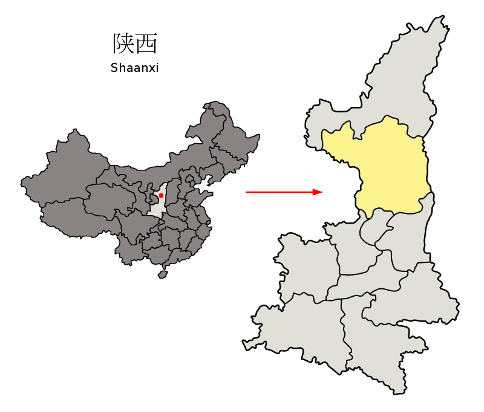
\includegraphics[width=0.6\textwidth]{figures/yanchang_map.png}
\caption{Location of Yanchang County in China}
\label{Figure: Yanchang}
\end{figure}

Yanchang's apple sector is dominated by late-maturing Fuji apples, which account for 85-90\% of total production, alongside smaller shares of mid-maturing (5-10\%) and early-maturing apples (around 5\%) \citep{yanchang2023}. Farm-gate prices range from 2.5 to 12 yuan per kilogram (\$0.16 to \$0.74 per pound) and fluctuate regularly, though yields per acre remain similar across varieties.  

The county consists of over 260 villages across eight rural townships, but cold storage infrastructure is limited. With just over 100 storage facilities, most villages lack direct access. Apple growers primarily use three types of cold storage: self-built facilities (capacity up to 50 tons) and small- and large-sized commercial facilities (up to 500 and 8000 tons, respectively). Only 1.3\% of farmers own storage, relying instead on rentals from township-run or merchant-operated facilities. Government-built storage facilities tend to be of lower quality than farmer-constructed ones. Farmers who build their own storage receive a 40\% government subsidy but must cover the remaining 60\% of the costs.  

Farmers without access to cold storage must sell their harvest within a month, while those with storage can extend sales into April or May, depending on market conditions. Apples stored at 1 degree Celsius in controlled environments maintain quality for several months \citep{Varela2005Shelf-life, Echeverria2004Relationships}. Storage adoption grants farmers temporal flexibility, allowing them to delay sales and potentially access a broader set of buyers, including direct-to-consumer retail markets, rather than being constrained to sell to middlemen. The ability to time sales strategically based on market competition and price fluctuations is a key determinant of storage's economic value.  



%------------------------------------------------------%
%------------------------------------------------------%
\section{Data}
\subsection{Sampling Procedure}
\noindent This study employs empirical tests using data from two rounds of a survey of 615 smallholder apple growers in Yanchang County, Central China, covering the 2024/2025 agricultural season. With Institutional Review Board (IRB) approval, the survey was conducted between October 10, 2024, and December 13, 2024. Since Fuji apple harvest in Central China concludes in mid-to-late October, followed immediately by storage and marketing decisions, this period provides a relevant window to analyze farmers' evolving market conditions.  

The survey was conducted in collaboration with the Yanchang-County Women's Federation (YWF), a local organization focused on public welfare and rural development. In coordination with the Yanchang County Agricultural Bureau, the YWF facilitated access to micro-level data on apple growers, enabling a structured sampling approach. A one-layer stratified random sampling method was applied based on geographical location. To ensure representativeness, the Yanchang County Agricultural Bureau determined sampling proportions for each town (30\%, 15\%, 15\%, 15\%, 10\%, 5\%, 5\%, and 5\%), reflecting the number and density of apple growers. Following these proportions, smallholder apple-growing households were randomly selected from village rosters.\footnote{In Yanchang County, over 95\% of apple growers cultivate no more than five acres, with large-scale commercial orchards being virtually nonexistent. The region is characterized by fragmented landholdings and household-based farming.}  

Smallholder apple growers are defined as those cultivating no more than 50 mu (about 8.24 acres) and deriving at least 90\% of their agricultural income from red Fuji apple production. A minimum of 10 farmers was selected per town to maintain sufficient sample sizes, though no village-level minimum was imposed. Interviews were conducted with household heads unless they were elderly and no longer part of the active labor force, in which case, the primary labor force member was interviewed.  

As indicated in Chapter~\ref{Chapter: descriptive chapter}, the cost of renting cold storage is charged based on weight rather than storage duration. It is therefore a one-time fee incurred at the time of apple storage, typically ranging from 0.4 to 0.6 RMB (5 to 8 cents in US dollars) per kilogram, depending on the type of cold storage facility. Considering that the average harvest price of apples in the region over the past decade has ranged from 4 to 8 RMB (0.55 to 1.10 US dollars) per kilogram, the cold storage rental fee (i.e., the storage cost) accounts for approximately 5\% to 15\% of the harvest price. In other words, if a farmer decides to store, considering other expenses like the transportation cost, he or she needs to get at least 10\% more than the harvest price to make the storage profitable.

%------------------------------------------------------%
\subsection{Measures of Farmers' Storage Usage and Procurement Competitiveness}
\noindent This study examines apple growers' cold storage usage and marketing timing decisions as key dependent variables. First, I define \texttt{Storage-Usage-Binary}, a binary indicator equal to 1 if a farmer used cold storage at harvest and 0 otherwise. Second, \texttt{Storage-Usage-Type} categorizes storage choices into four groups: \textit{Not\_use} (no storage), \textit{Rent\_large} (rented large-scale commercial storage), \textit{Rent\_small} (rented small-scale storage), and \textit{Self\_built} (self-owned storage). Third, \texttt{Time-to-Sell} measures the delay between harvest and sale, effectively capturing storage duration. Sales occurring in October are classified as 1-4 weeks post-harvest, November as 5-8 weeks, and so forth, yielding interval-censored data with four predefined selling-time intervals: 1-4, 5-8, 9-12, and 13-28 weeks. Figure \ref{Figure: selling weeks distribution} illustrates the distribution of selling weeks by storage type.  

\begin{figure}[H]
\centering
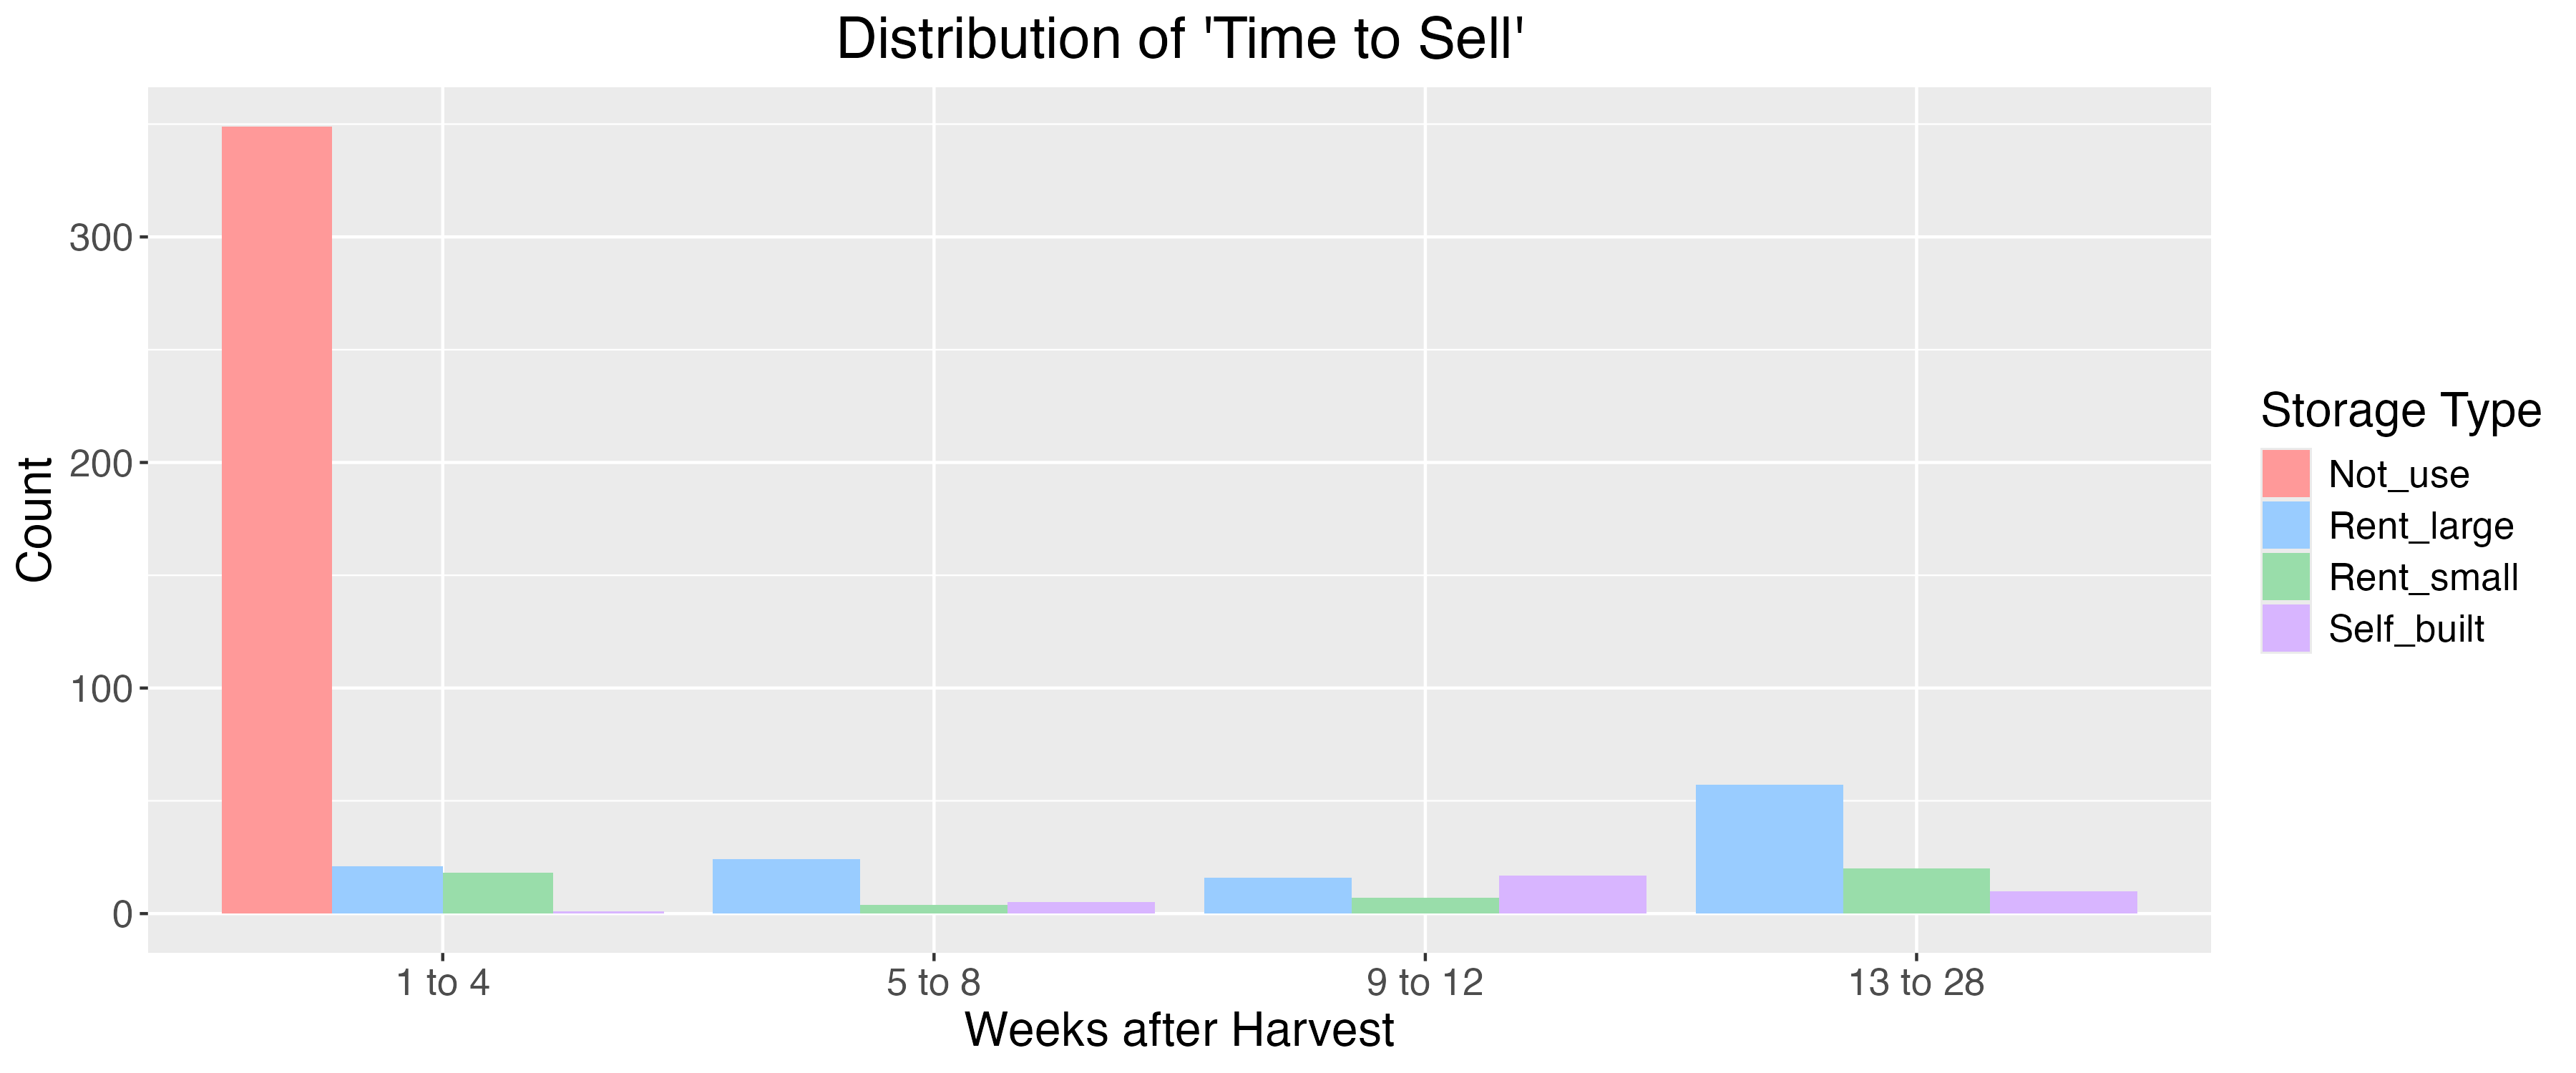
\includegraphics[width=1\textwidth]{figures/selling_weeks_distribution.png}
\caption{Distribution of Selling Weeks by Storage Type}
\label{Figure: selling weeks distribution}
\end{figure}

To capture inter-temporal variations in buyer power and market competitive conditions, farmers reported:
\begin{enumerate}
    \item Their subjective assessment of buyer competition at harvest (\texttt{Subjective buyer competitiveness}, measured on a 1-5 scale);
    \item Their expectations regarding changes in the number of traders over the next three months (recorded as \texttt{Expect more buyers} and \texttt{Expect fewer buyers}).
\end{enumerate}

Additionally, the survey collected data on farmers' agricultural income, production costs, storage expenses, and demographic characteristics to assess the welfare implications of storage adoption.  

To complement these farmer-level insights with market-level dynamics, a buyer survey was conducted in December 2024. This survey targeted 15 buyers, including the top five most influential local traders, and collected data on:
\begin{enumerate}
    \item The specific villages each buyer visited during the October harvest;
    \item The cold storage facilities from which they had procured apples over the preceding two months.
\end{enumerate}
These responses allow for the construction of an objective measure of buyer concentration which might serve as a proxy of inter-temporal buyer competition. Inspired by \cite{macchiavello2021competition}, who used the number of coffee mills within a 10 km radius as a competition metric in Rwanda's coffee industry, I define \texttt{Number of buyers} as the count of traders visiting each village at harvest.  


%------------------------------------------------------%
\subsection{Measures of Farmers' Risk Aversion and Liquidity Constraint}
\noindent Building on \cite{jin2024losses}, whose fieldwork location closely aligns with that of this study, apple growers' risk preferences are measured using two complementary methods: a self-reported risk preference scale and a behavioral measure based on a Holt-Laury-type lottery game. The combination of subjective and incentivized approaches provides a robust assessment of farmers' risk attitudes. Liquidity constraints are defined following \cite{albuquerque2024market} and \cite{stephens2011incomplete}, classifying farmers as liquidity-constrained if they report both difficulty accessing credit and a need to sell immediately at harvest to meet urgent cash requirements.

\subsubsection{Self-Reported Risk Preference}  
\noindent Following \cite{dohmen2011individual}, general risk attitudes are elicited through a five-point scale, where 1 indicates \textit{``extreme risk aversion''} and 5 represents \textit{``very risk loving''}. While inherently subjective and potentially influenced by social and peer effects, self-reported measures provide useful insights into farmers' perceptions of risk, which likely influence investment, production, and financial decisions.  

\subsubsection{Holt-Laury-Type Lottery Game}  
\noindent To complement the self-assessment, a modified Holt-Laury-type lottery game was implemented. Apple growers were asked how much they would be willing to pay to enter a 50-50 lottery with a potential payout of 200 CNY or nothing. This adapts the \textit{multiple price list (MPL) choice task} from \cite{brick2012risk}, a variation of the Holt-Laury method \citep{holt2002risk}. Participants chose whether to pay varying entry fees (20-120 CNY), effectively selecting between a \textit{safe} (keeping the money) and a \textit{risky} (entering the lottery) option.  

This approach is well-suited for field settings, being simple to administer while using real monetary stakes to elicit truthful responses. Different willingness-to-pay (WTP) values correspond to varying expected values and degrees of risk aversion, as shown in Table \ref{tab:experiment_design}.  

\begin{table}[H]
    \centering
    \footnotesize 
    \caption{Risk Preference Experiment Design: A Head-Tail Lottery Game}
    \renewcommand{\arraystretch}{1.2}
    \begin{tabular}{cccccc}
        \toprule
        \textbf{Option} & \textbf{Willingness to Pay} & \textbf{Outcome} & \textbf{EV$^{A}$--EV$^{B}$} & \textbf{CRRA Ranges} & \textbf{CRRA Adjusted}\\
        \midrule
        1 & 120 CNY & 200 CNY or 0 & 20 CNY & $-0.4 < \gamma < 0$  & $\gamma = -0.2$\\
        2 & 100 CNY & 200 CNY or 0 & 0 CNY & $0 < \gamma < 0.2$  & $\gamma= 0.1$ \\
        3 & 80 CNY & 200 CNY or 0 & -20 CNY & $0.2 < \gamma < 0.4$  & $\gamma= 0.3$ \\
        4 & 60 CNY & 200 CNY or 0 & -40 CNY & $0.4 < \gamma < 0.6$  & $\gamma= 0.5$ \\
        5 & 40 CNY & 200 CNY or 0 & -60 CNY & $0.6 < \gamma < 0.7$  & $\gamma=0.6$ \\
        6 & 20 CNY & 200 CNY or 0 & -80 CNY & $0.7 < \gamma$  & $\gamma= 0.9$ \\
        \bottomrule
    \end{tabular}
    \label{tab:experiment_design}
    \vspace{0.5em}
    \small Notes: EV = Expected Value. CRRA = Coefficient of Constant Relative Risk Aversion.
\end{table}

While the head-tail lottery design provides a tractable way to elicit \textit{point estimates} of risk preferences in the field, the implied CRRA coefficients are typically much smaller than the range used in simulation exercises. For instance, the experimental design in Table~\ref{tab:experiment_design} maps observed willingness-to-pay decisions into CRRA values that mostly fall below 1, consistent with evidence from other MPL-style tasks in agricultural settings. By contrast, the simulations in Section~\ref{Section: Base Model Numerical Analysis} in Chapter 4 vary $\gamma$ over a wider domain, $[0,10]$, to capture the full spectrum of heterogeneity documented in the literature---from risk neutrality to extreme risk aversion. In practice, the field experiment serves to benchmark farmers' risk preferences around the lower end of this spectrum, while the simulation framework explores the implications of more severe risk aversion that, although less common, is empirically observed in some rural populations.\footnote{Empirical studies using similar elicitation tasks often report CRRA values in the range of 0.5--3 (see, e.g., \cite{liu2013time}).}



\subsubsection{Estimating Risk Aversion Using CRRA}  
\noindent The highest entry price a participant is willing to pay provides insight into their risk preference. Following \cite{chiappori2011relative}, who found that individuals generally exhibit constant relative risk aversion (CRRA), a CRRA utility function is assumed:  
\[
U(x) = \frac{x^{1-\gamma}}{1 - \gamma}
\]  
where \( \gamma \) represents the risk aversion coefficient. Under this specification, \( \gamma > 0 \) implies risk aversion, \( \gamma = 0 \) indicates risk neutrality, and \( \gamma < 0 \) reflects risk-seeking behavior. Columns 5 and 6 in Table \ref{tab:experiment_design} present the corresponding CRRA ranges and adjusted CRRA values. These estimates allow for a quantitative assessment of farmers' risk aversion, which is critical for understanding storage decisions and responses to market uncertainty.  

\subsubsection{Liquidity Constraint}  
\noindent The binary variable \texttt{Liquidity constrained} equals 1 if a farmer reports both difficulty accessing credit and an urgent need to sell at harvest to cover immediate expenses (e.g., school tuition or medical costs). This measure refines and extends approaches used by \cite{albuquerque2024market} and \cite{stephens2011incomplete}, who define credit access as a proxy for liquidity constraints.  

Only a small fraction of surveyed farmers (about 15\%) meet the criteria for liquidity constraints, with no strong correlation between liquidity constraints and storage or selling decisions. One possible explanation is that the study region, located in Central China, is a designated provincial rural revitalization area, attracting both state- and private-owned financial institutions that provide inclusive credit access.  

Additionally, insights from interviewed local villagers suggest that past exposure to natural disasters, such as hailstorms, has fostered a strong savings culture. Farmers in Yanchang County prioritize financial resilience, making them less likely to engage in distress sales. While liquidity constraints affect some growers, this measure primarily captures relative financial strain rather than absolute financial distress.  




%------------------------------------------------------%
\subsection{Descriptive Statistics}  
\noindent The final dataset consists of 549 smallholder apple-growing households in Central China, of whom 200 used cold storage during the 2024-2025 agricultural year. Among these, 33 stored apples in self-built facilities, 49 rented small-scale commercial storage, and 118 opted for large-scale commercial storage.  

\begin{figure}[htp]
\centering
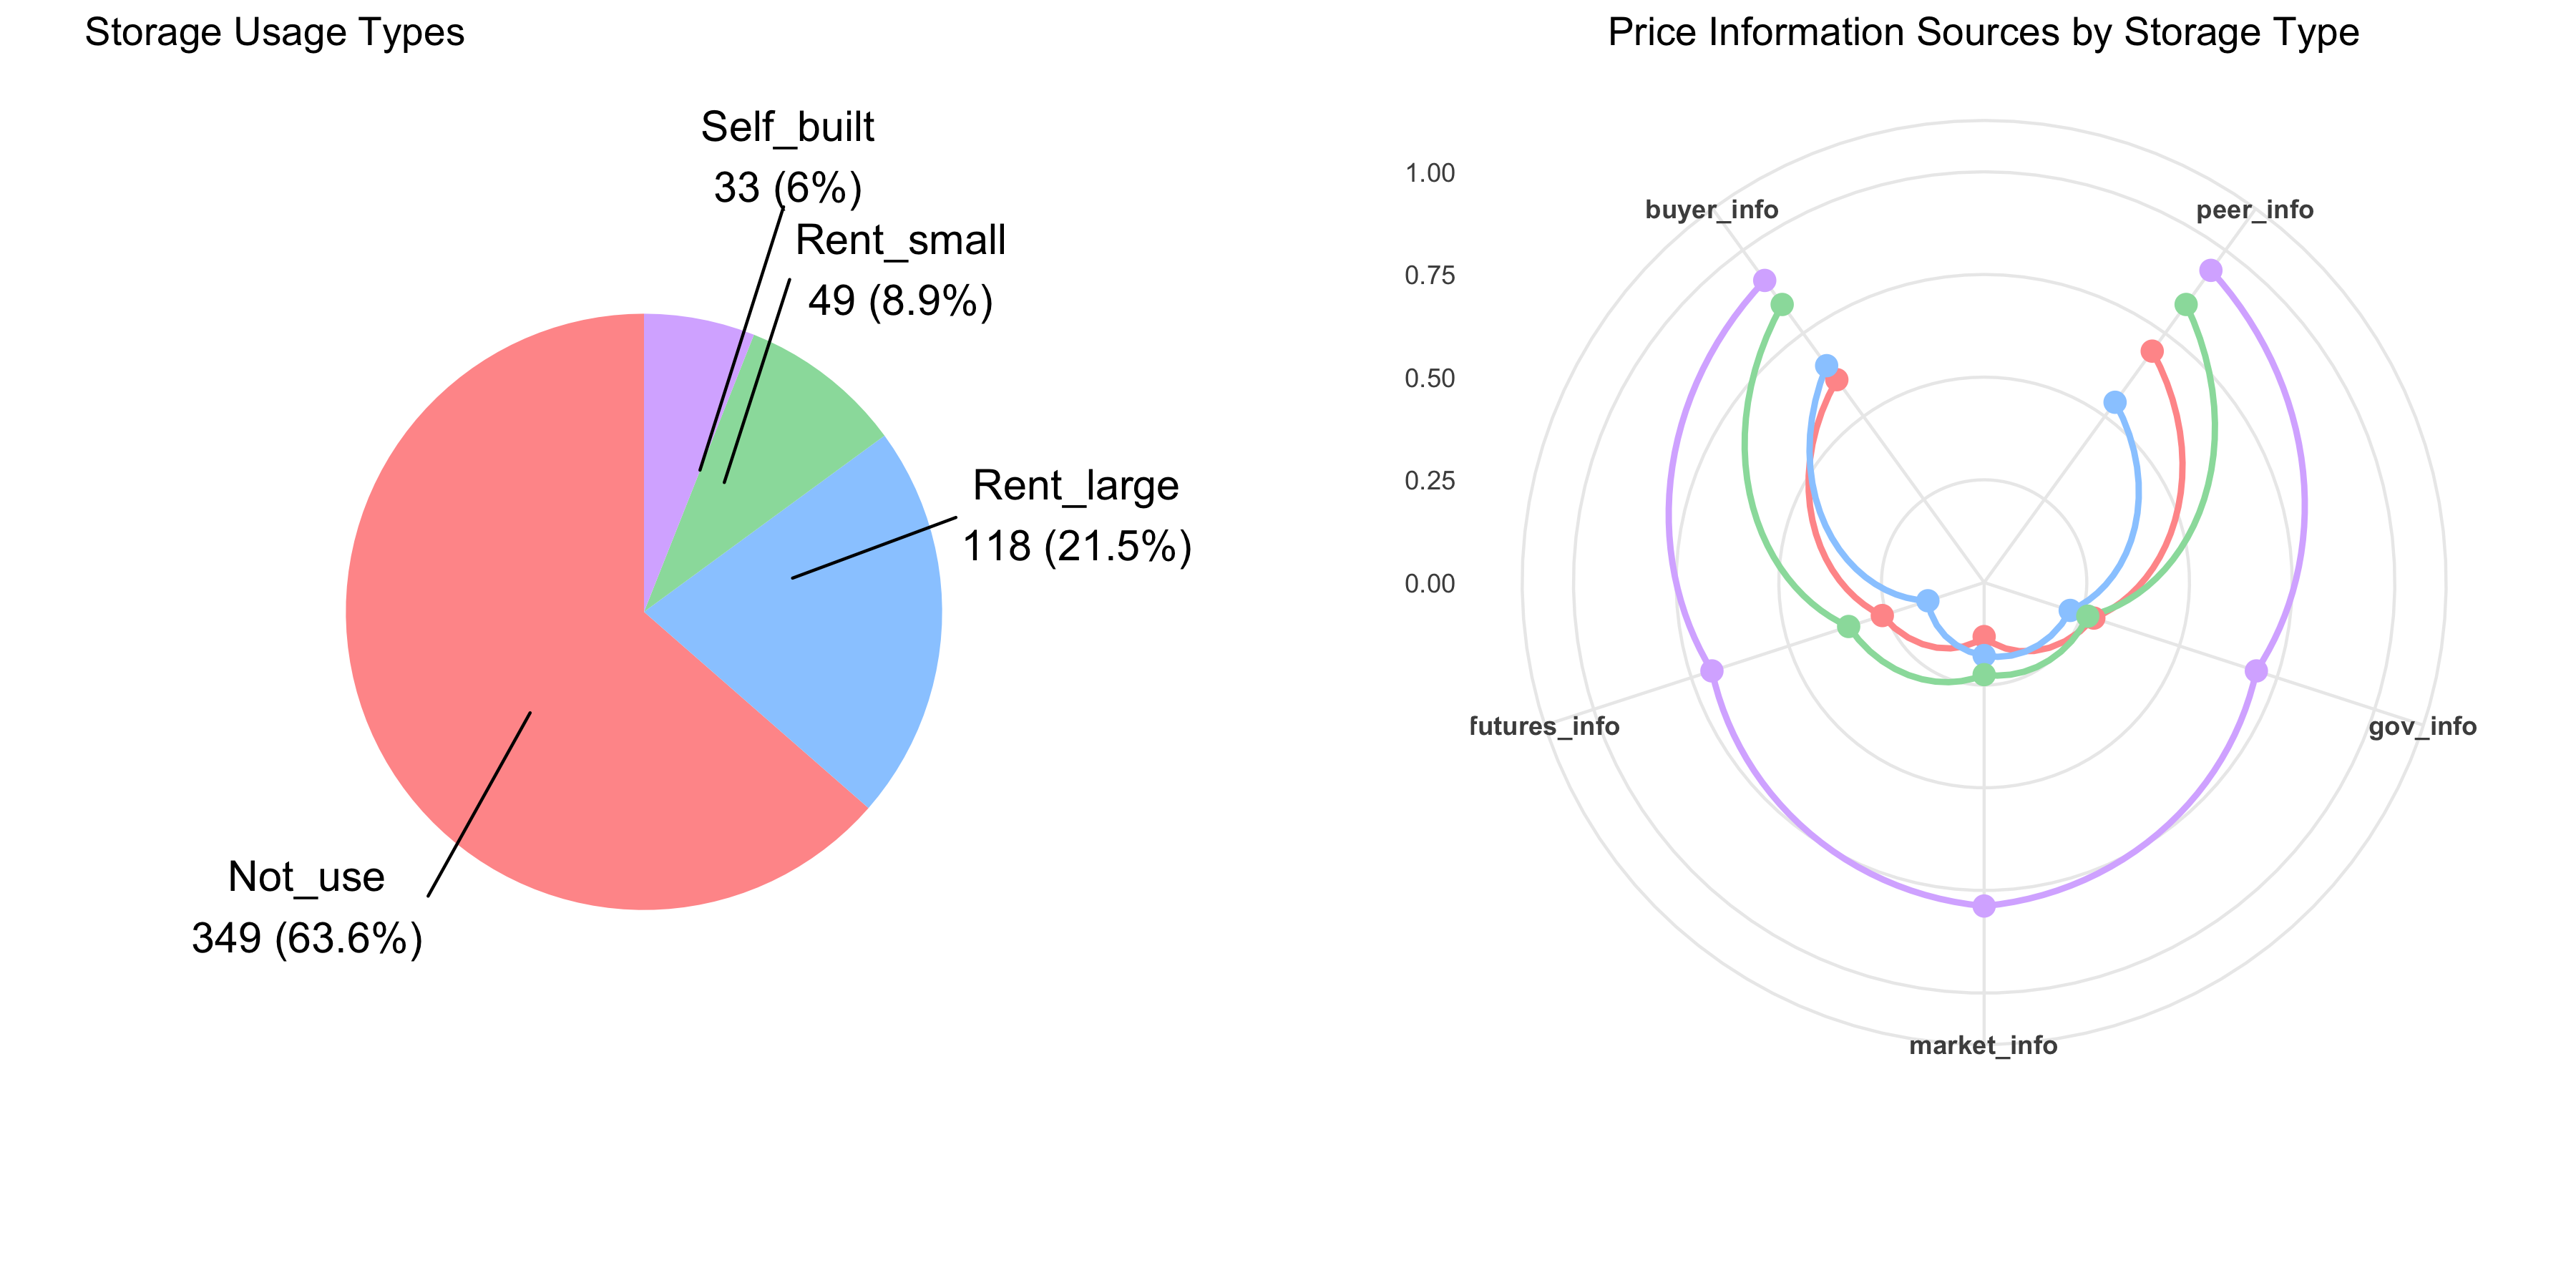
\includegraphics[width=1\textwidth]{figures/storage_usage_analysis_soft_colors.png}
\caption{Distribution of Storage Usage Types and Their Price Information Sources}
\label{Figure: pie and radar chart}
\end{figure}

Figure \ref{Figure: pie and radar chart} illustrates the distribution of storage usage and the sources of price information. The radar chart on the right highlights variations in information-seeking behavior across groups. Growers with self-built storage (purple) are the most active in gathering market insights, suggesting a strong need for independent decision-making. Those using small-scale (green) and large-scale (blue) commercial storage engage at moderate but balanced levels, likely reflecting a reliance on both direct transactions and broader market signals. In contrast, growers selling immediately at harvest (red) show minimal engagement, primarily depending on buyer and peer information.  

These differences in search activity are also reflected in the composition of price information sources. Self-built storage users prioritize market data while supplementing it with buyer and peer sources, aligning with their need to optimize sales timing. Small-scale commercial users rely heavily on buyer and peer information, reflecting localized transactions and network-based decision-making. Large-scale commercial users adopt a more diversified approach, integrating multiple sources to manage risk and maximize returns. Growers selling at harvest depend narrowly on immediate contacts for pricing, underusing institutional sources such as government data and futures markets. This pattern suggests a general preference for informal, experience-based price discovery over structured, institutional sources.

\begin{table}[H]
\centering
\caption{Summary Statistics by Storage Usage}
\label{tab: summary statistics}
\resizebox{\textwidth}{!}{%
\begin{tabular}{lccccc}
\toprule
 & \multicolumn{2}{c}{Storage Users} & \multicolumn{2}{c}{Non-Users} & Difference \\
\cmidrule(lr){2-3} \cmidrule(lr){4-5}
Variable & Mean & SD & Mean & SD & t-statistic \\
\midrule
\multicolumn{6}{l}{\textbf{Panel A: Farmer Demographics}} \\
Age (years) & 56.87 & (9.57) & 60.35 & (9.63) & -4.09*** \\
Household size (persons) & 2.71 & (1.21) & 2.58 & (1.10) & 1.24 \\
Labor size (persons) & 1.74 & (0.71) & 1.60 & (0.66) & 2.20** \\
Highest education (level) & 1.96 & (0.67) & 1.81 & (0.76) & 2.35** \\
Family ever village leader (0/1) & 0.24 & (0.43) & 0.06 & (0.24) & 5.37*** \\
Liquidity constrained (0/1) & 0.15 & (0.36) & 0.16 & (0.37) & -0.17 \\
\addlinespace
\multicolumn{6}{l}{\textbf{Panel B: Production and Consumption}} \\
Apple yield (tons) & 11.08 & (7.56) & 11.68 & (14.12) & -0.64 \\
Land size (acre) & 2.60 & (1.70) & 1.72 & (0.99) & 6.69*** \\
Bad apple ratio & 2.31 & (1.20) & 2.02 & (1.18) & 2.78*** \\
Apple income (USD) & 10127.22 & (6108) & 8289 & (6465) & 3.32*** \\
Total income (USD) & 10919 & (6445) & 8990 & (7334) & 3.21*** \\
Labor cost (USD) & 1911 & (1593) & 1343 & (1258) & 4.33*** \\
Family consumption (USD) & 7117 & (8899) & 5059 & (3869) & 3.11*** \\
\addlinespace
\multicolumn{6}{l}{\textbf{Panel C: Storage and Risk-Related Factors}} \\
Car/truck ownership (0/1) & 0.14 & (0.35) & 0.04 & (0.20) & 3.61*** \\
Natural disaster insurance (0/1) & 0.35 & (0.48) & 0.33 & (0.47) & 0.49 \\
Price insurance (0/1) & 0.62 & (0.49) & 0.65 & (0.48) & -0.78 \\
CRRA adjusted (coef) & 0.09 & (0.37) & 0.36 & (0.45) & -7.75*** \\
Storage in village (0/1) & 0.38 & (0.49) & 0.20 & (0.60) & 3.74*** \\
Far to small storage (0/1) & 0.52 & (0.50) & 0.79 & (0.41) & -6.71*** \\
Far to large storage (0/1) & 0.89 & (0.32) & 0.91 & (0.28) & -1.07 \\
Storage for wider marketing (0/1) & 0.88 & (0.33) & 0.30 & (0.46) & 16.90*** \\
Storage as bargaining tool (0/1) & 0.80 & (0.40) & 0.29 & (0.46) & 13.79*** \\
\addlinespace
\multicolumn{6}{l}{\textbf{Panel D: Marketing}} \\
Highest price per pound (USD/lb) & 0.41 & (0.09) & 0.38 & (0.10) & 3.94*** \\
Good price per pound (USD/lb) & 0.40 & (0.08) & 0.37 & (0.10) & 3.29*** \\
WeChat selling (0/1) & 0.15 & (0.36) & 0.00 & (0.00) & 6.04*** \\
Relational selling (0/1) & 0.12 & (0.33) & 0.14 & (0.35) & -0.78 \\
Contract selling (0/1) & 0.40 & (0.49) & 0.26 & (0.44) & 3.32*** \\
\addlinespace
\multicolumn{6}{l}{\textbf{Panel E: Market Competitive Conditions}} \\
Expect more buyers (0/1) & 0.46 & (0.50) & 0.06 & (0.23) & 10.75*** \\
Expect fewer buyers (0/1) & 0.16 & (0.39) & 0.19 & (0.39) & -0.90 \\
Number of buyers at harvest (count) & 3.83 & (2.45) & 3.12 & (1.91) & 3.51*** \\
Subjective buyer competitiveness (1/5) & 2.92 & (0.84) & 3.06 & (0.69) & -2.08** \\
\hline
\hline
Observations & 200 & & 349 & & 549 \\
\bottomrule
\end{tabular}% 
} % End of resizebox 
\begin{tablenotes} 
\item \textit{Notes:} The table presents means and standard deviations (in parentheses) for each variable by group. T-statistics from two-sample t-tests are reported to indicate statistical significance of differences between groups. Significance levels are denoted by asterisks: * p$<$0.1, ** p$<$0.05, *** p$<$0.01. In addition, monetary values have been converted from Chinese Yuan (RMB) to US Dollars (USD), land area from mu to acres, and apple prices from RMB/kg to USD/pound using appropriate conversion rates. 
\end{tablenotes} 
\end{table}


The subset of 200 storage users provides a key sample for analyzing storage-related decision-making in greater detail. Table \ref{tab: summary statistics} presents descriptive statistics comparing storage users and non-users across key demographic, production, marketing, and market competition variables. Significant differences emerge in demographic characteristics, with storage users being younger on average (56.87 vs. 60.35 years, $p < 0.01$), having slightly larger household labor forces (1.74 vs. 1.60 persons, $p < 0.05$), and being more likely to have a family member who has served as a village leader (24\% vs. 6\%, $p < 0.01$). While education levels are marginally higher for storage users (1.96 vs. 1.81 on a categorical scale, $p < 0.05$), liquidity constraints appear similar across both groups. These findings suggest that access to storage may be associated with leadership connections and greater household labor availability, which could facilitate better market participation and bargaining power. The rightmost column reports t-statistics from two-sample t-tests to indicate whether differences between groups are statistically significant.  

In terms of production and income, storage users operate on significantly larger landholdings (2.60 vs. 1.72 acres, $p < 0.01$) and report higher apple-related earnings (\$10,127 vs. \$8,289, $p < 0.01$). However, their yields per acre do not significantly differ from non-users. Storage users also face a slightly higher proportion of bad apples (2.31 vs. 2.02, $p < 0.01$), suggesting that storage may play a role in mitigating losses from quality deterioration. Additionally, storage users incur greater labor costs (\$1,911 vs. \$1,343, $p < 0.01$) and spend more on family consumption (\$7,117 vs. \$5,059, $p < 0.01$).  

Storage access appears closely linked to marketing strategy and market expectations. A significantly larger proportion of storage users engage in relational selling (40\% vs. 26\%, $p < 0.01$), use WeChat for sales (15\% vs. 0\%, $p < 0.01$), and expect more buyers in the future (46\% vs. 6\%, $p < 0.01$), reflecting greater confidence in market expansion. Moreover, storage enables broader marketing strategies, with 88\% of storage users explicitly storing apples for wider marketing (vs. 30\% among non-users, $p < 0.01$) and 80\% using storage as a bargaining tool (vs. 29\%, $p < 0.01$). These differences suggest that storage is not only a means of extending the sales period but also a strategic tool for improving price negotiation and expanding market reach, reinforcing its role in enhancing producer bargaining power.  

\begin{figure}[htp]
\centering
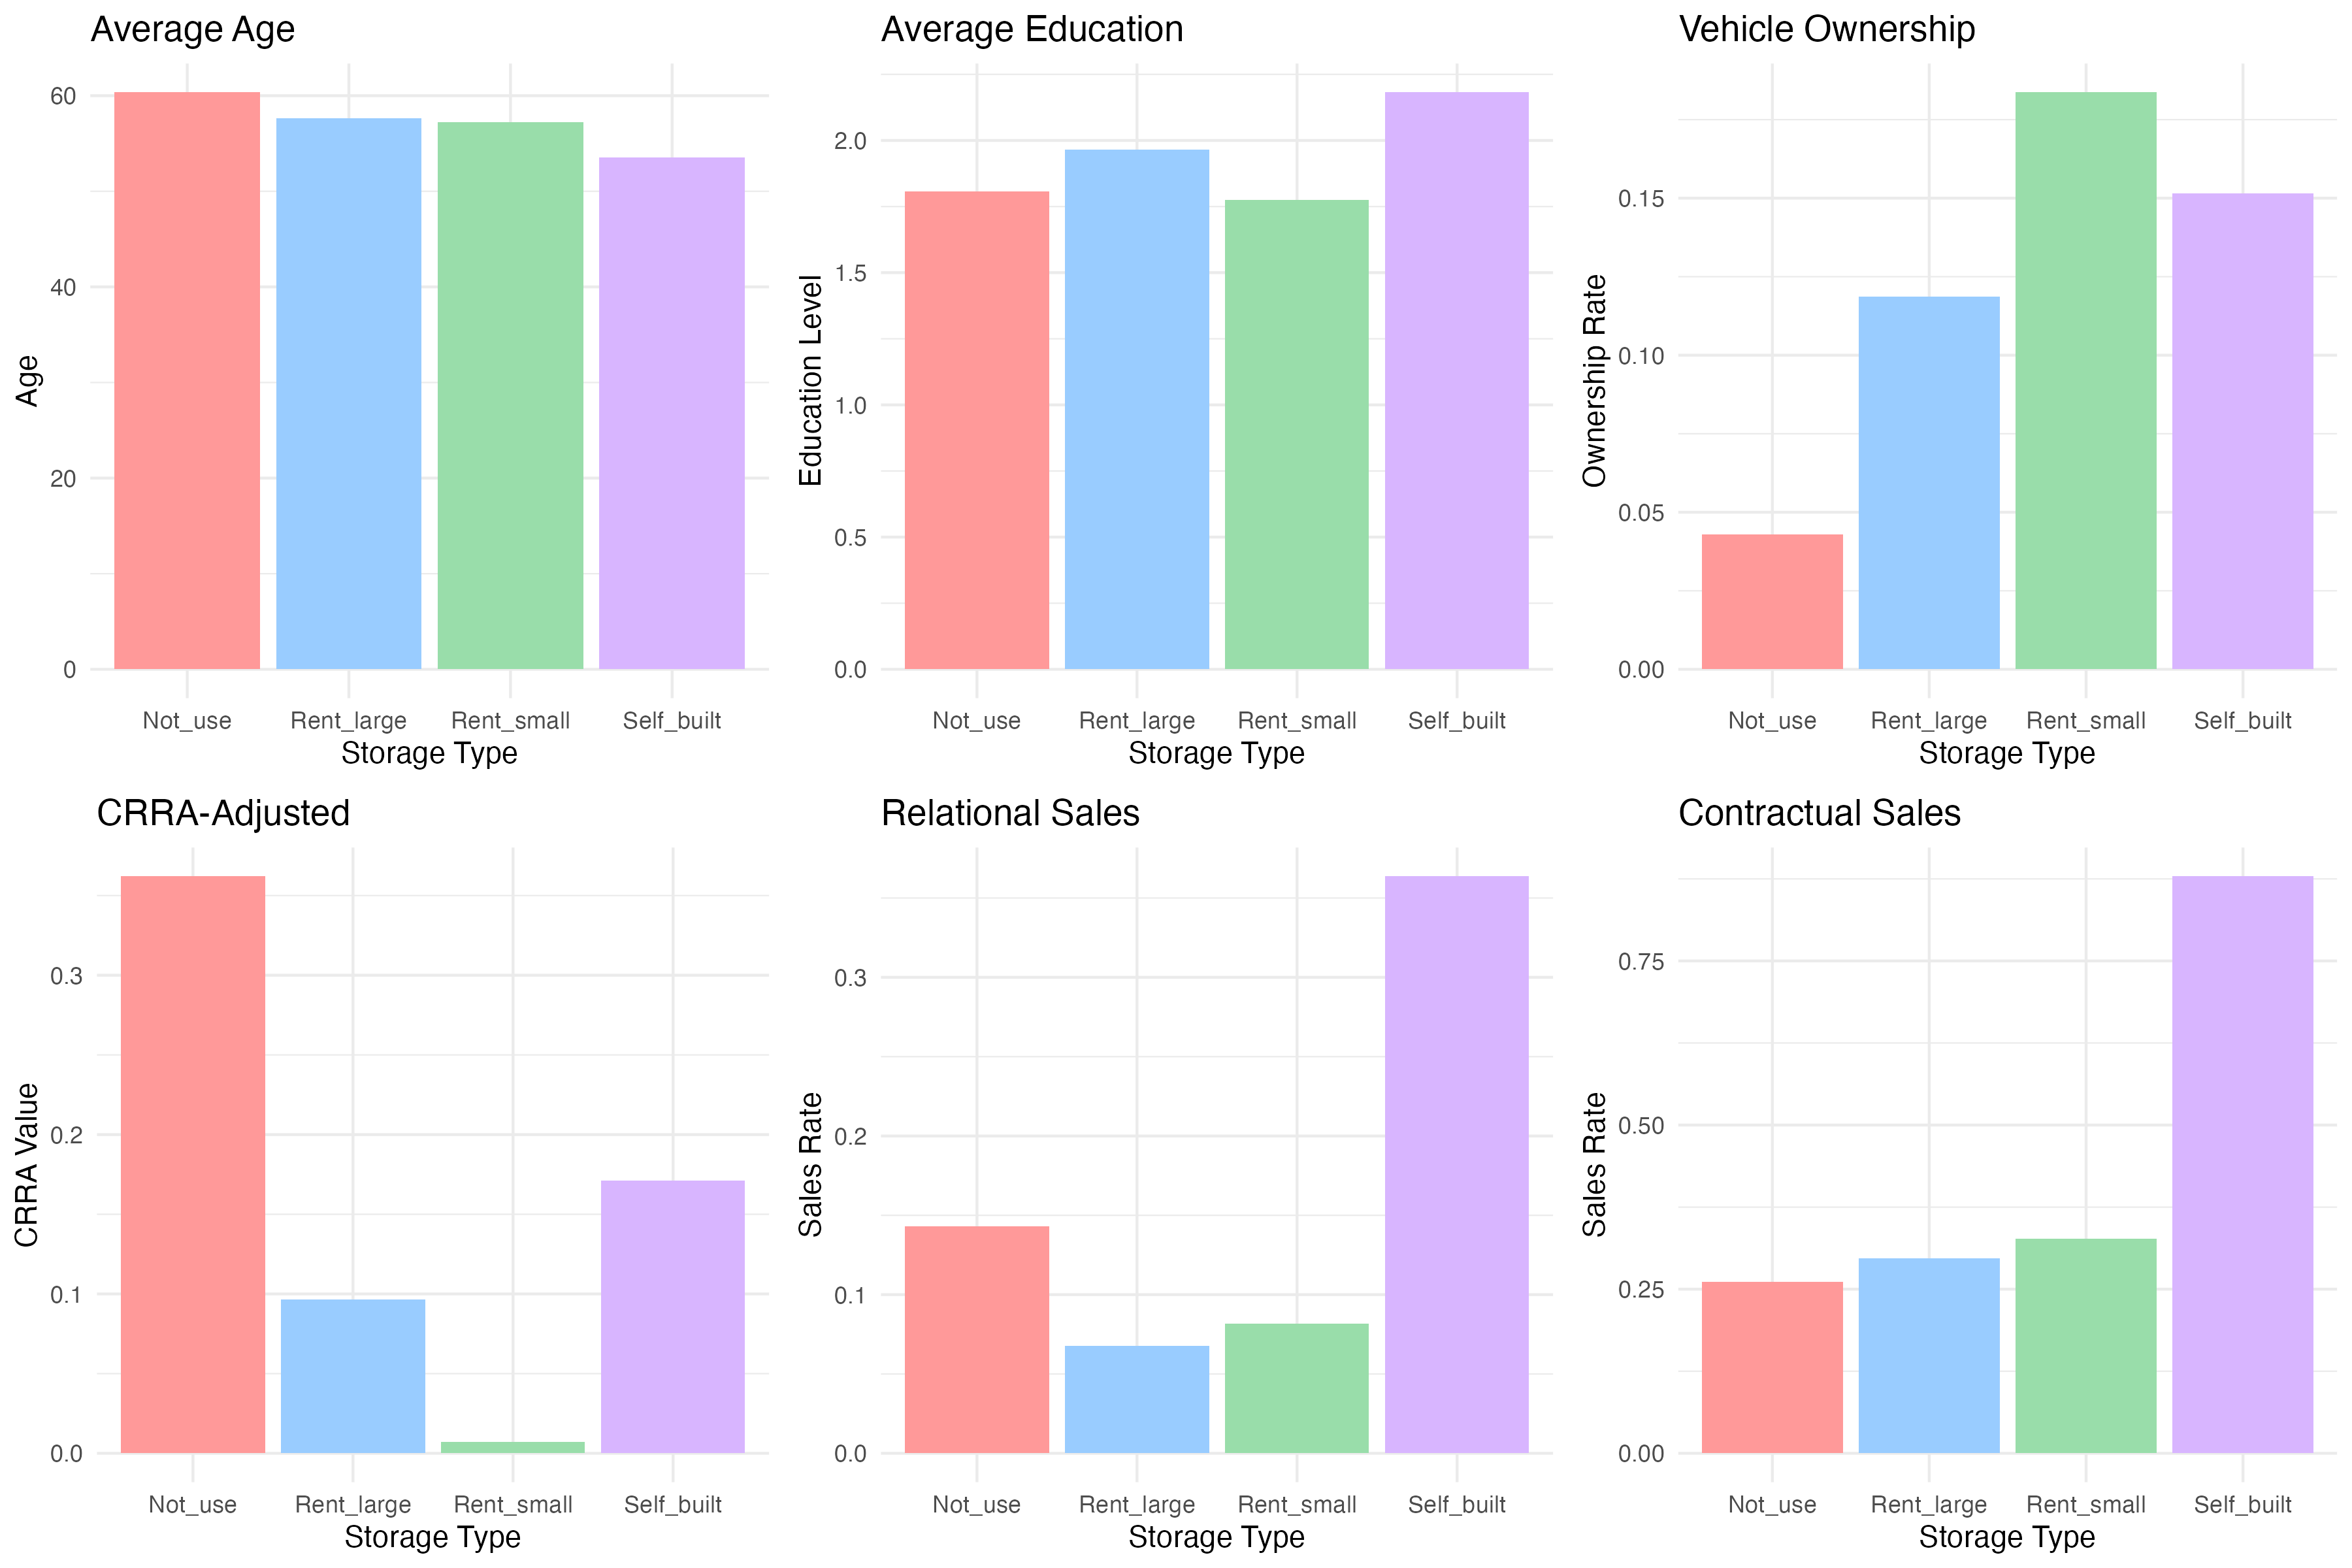
\includegraphics[width=1\textwidth]{figures/combined_storage_metrics.png}
\caption{Demographics by Storage Type}
\label{Figure: Demographics by Storage Type}
\end{figure}

Furthermore, Figure \ref{Figure: Demographics by Storage Type} compares key demographic characteristics across four storage usage categories: non-users, users with self-built storage, and users renting small- and large-scale commercial storage facilities. The figure highlights differences in six key variables: age, education level, car/truck ownership, risk aversion (adjusted CRRA), and participation in relational and implicit contractual sales.   

Table \ref{tab: summary statistics} shows that non-storage farmers receive an average highest price of \$0.38 per pound (6.12 RMB/kg), with an average transaction price of \$0.37 per pound (5.96 RMB/kg), both slightly lower than those of storage users. As illustrated in Figure \ref{Figure: selling price bubble}, non-storage farmers are constrained to selling at harvest (October), when transaction prices exhibit high volatility before stabilizing in subsequent months. Prices typically rise in November and December, though sales volumes decline. Storage users who delay sales achieve on average a price premium of roughly \$0.03 per pound ($\approx$ 0.45 RMB/kg) over non-storers. Given that reported storage costs fall in the same range (0.40-0.50 RMB/kg), the average net payoff to storage in this survey year was close to zero. Nevertheless, storers retained the opportunity to capture substantially higher returns in certain months, with realized prices occasionally reaching \$0.50--\$0.60 per pound ($\approx$ 7.80--9.4 RMB/kg) in December. This highlights the role of storage as a risky inter-temporal strategy: while not systematically profitable on average once costs are deducted, it provided upside potential for some farmers depending on timing and market conditions.


\begin{figure}[H]
\centering
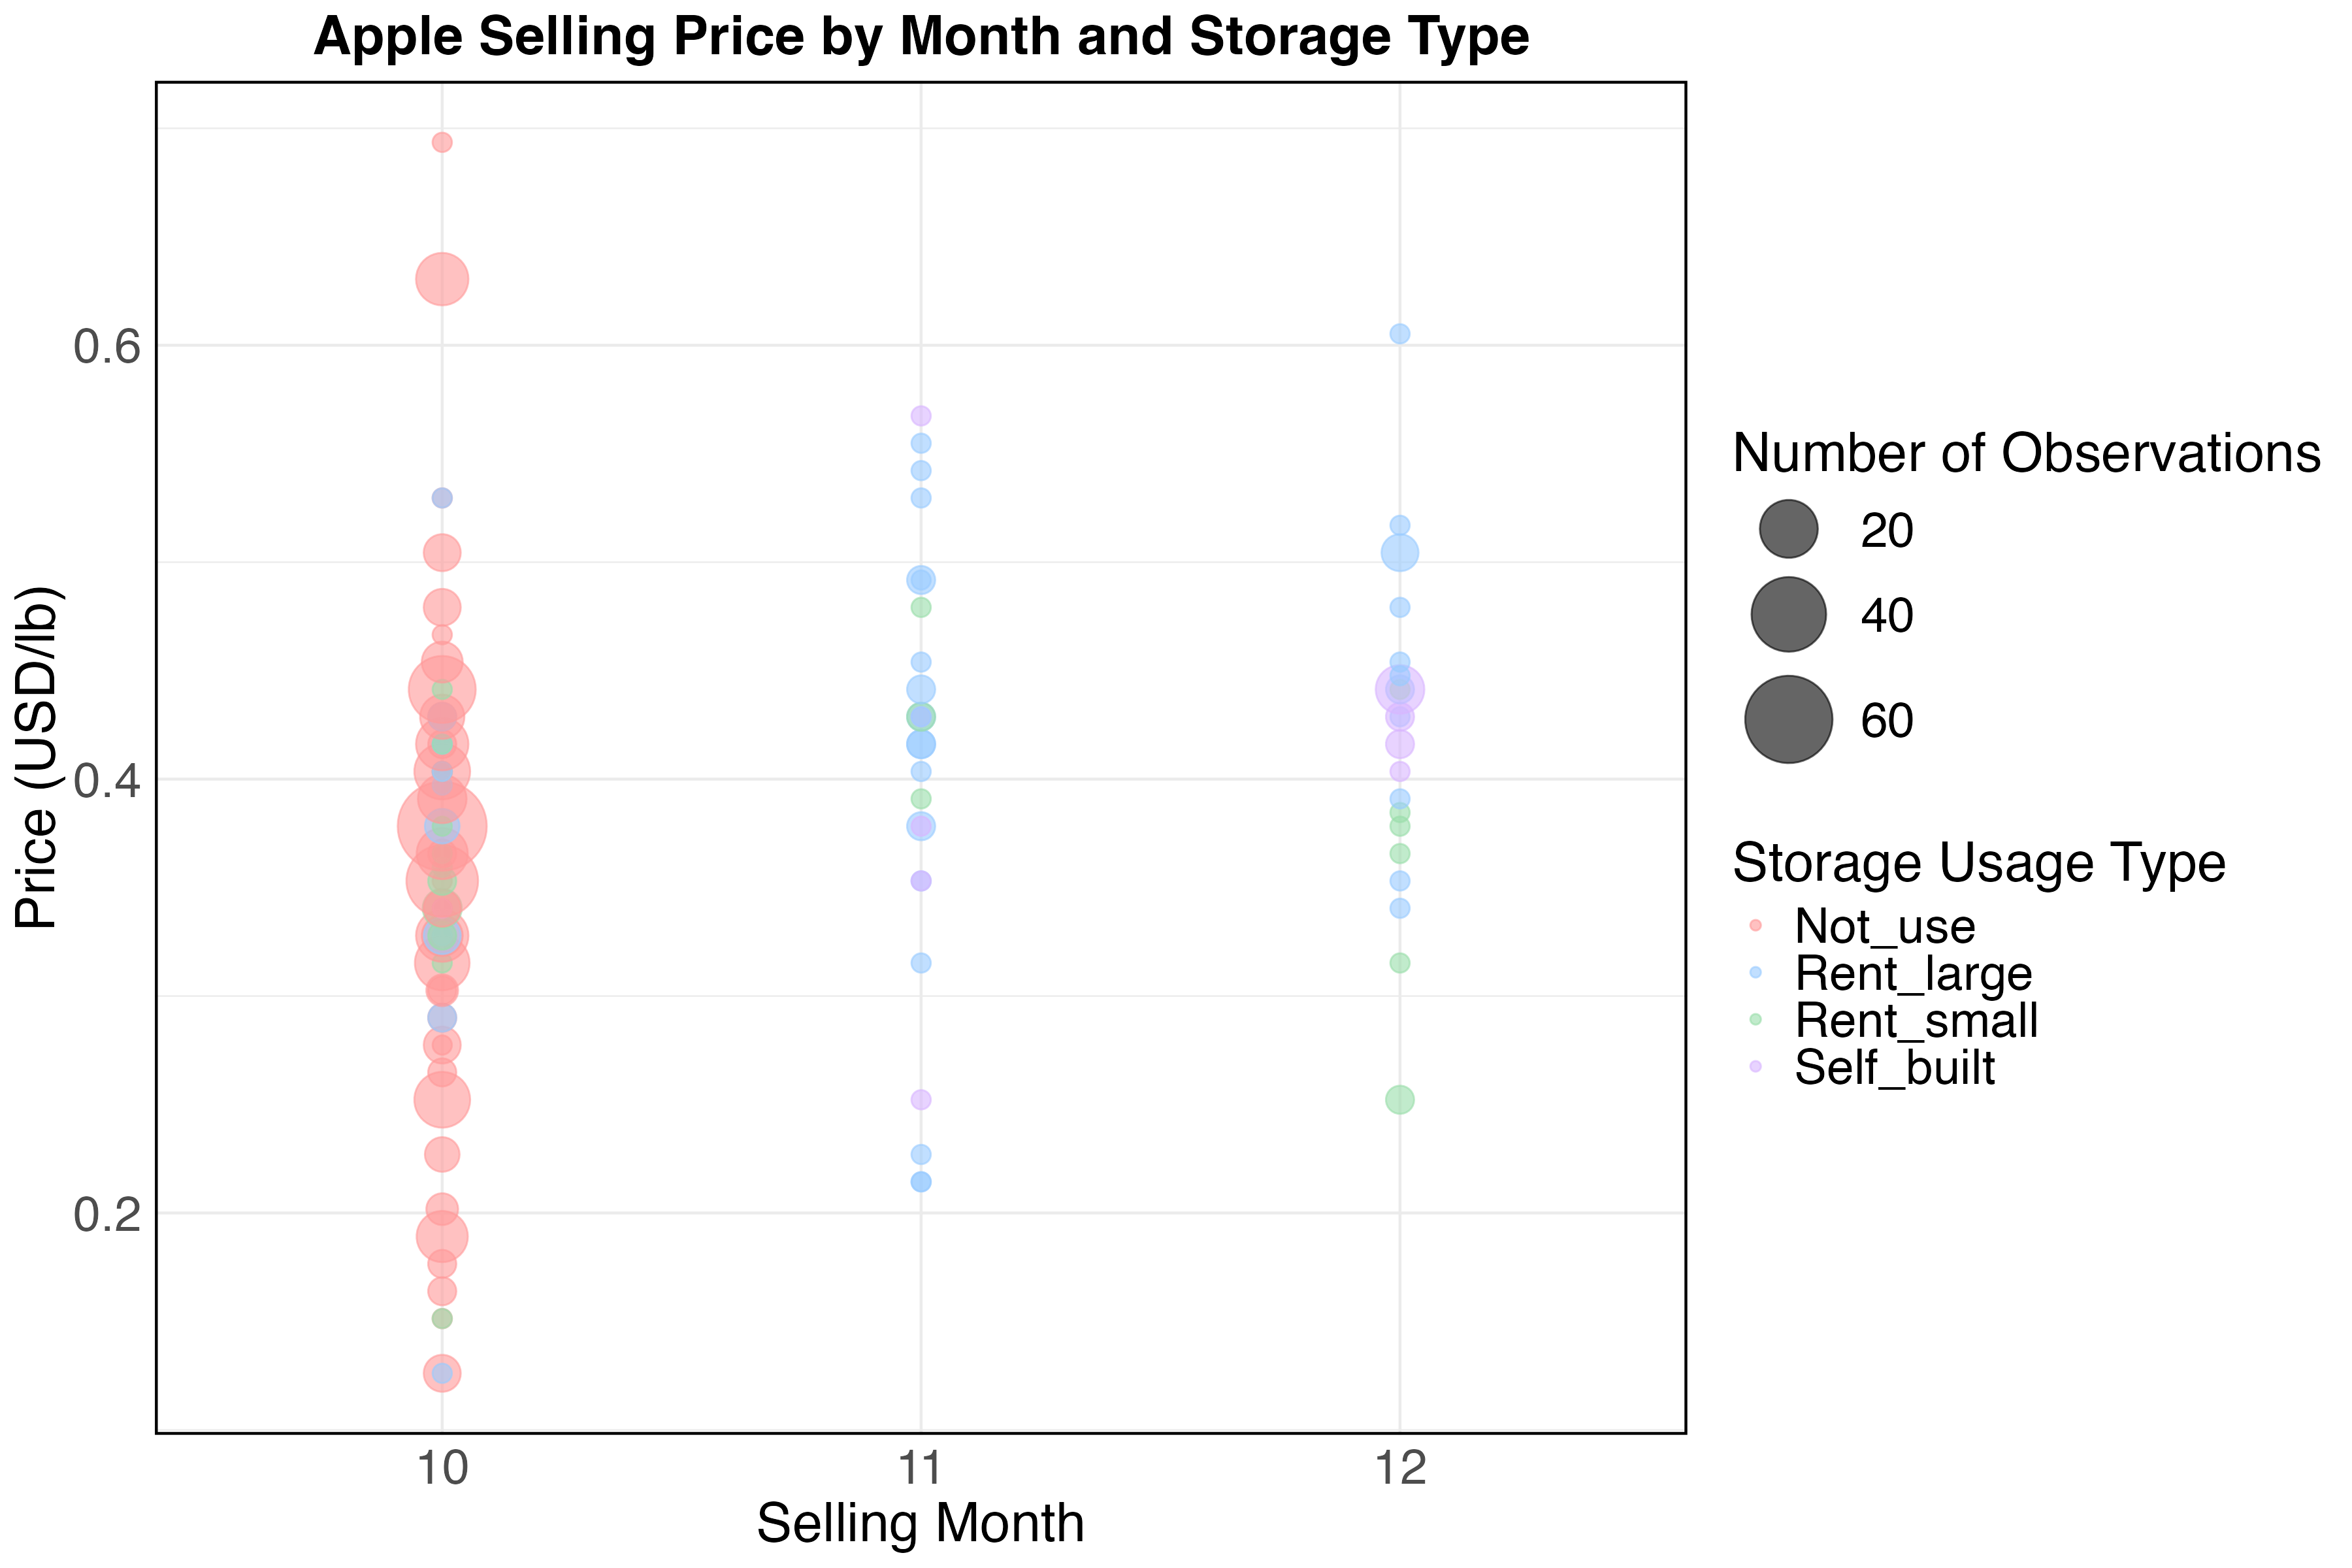
\includegraphics[width=1.05\textwidth]{figures/apple_price_bubble_plot.png}
\caption{Apple Selling Price by Month and Storage Type}
\label{Figure: selling price bubble}
\end{figure}

Despite the potential benefits of storage, many farmers opt not to store their produce, often due to negative past experiences. Table \ref{tab:non_storage_reasons} summarizes the primary reasons cited by 349 non-storage farmers. The most frequently mentioned concern, reported by 60.75\% of respondents, is skepticism about future price increases. Beyond price uncertainty, 28.65\% of farmers perceive storage as too risky, citing potential losses from spoilage, market downturns, or unreliable storage access. Additionally, 22.92\% report high storage costs as a prohibitive factor. A smaller group (8.02\%) indicates that pre-arranged sales eliminate the need for storage. These findings suggest that, while cold storage could improve farmers' marketing flexibility, adoption is hindered by market uncertainty, perceived financial and logistical concerns, and established pre-arranged sales.  


\begin{table}[H]
    \centering
    \footnotesize
    \caption{Reasons for Not Using Storage Facilities}
    \label{tab:non_storage_reasons}
    \resizebox{\textwidth}{!}{%
        \begin{tabular}{lcccc}
            \toprule
            \textbf{Reason} & High Storage Costs & Pre-arranged sale & Cannot Sell High Later & Too Risky \\
            \midrule
            \textbf{Percentage} & 22.92\% & 8.02\% & 60.75\% & 28.65\% \\
            \bottomrule
        \end{tabular}%
        }
        \begin{tablenotes}
            \item \textit{Notes:} This table presents the reasons provided by the 349 farmers who do not use storage facilities, expressed as percentages of total non-storage farmers.
        \end{tablenotes}
\end{table}


%------------------------------------------------------%
%------------------------------------------------------%
\section{Empirical Specification}
\subsection{Storage Decisions: Buyers' Competitiveness at Harvest}
\noindent 
This section presents the results of a logistic regression model with town-level fixed effects examining the determinants of binary storage usage. The dependent variable is whether an individual engages in storage ($S_i = 1$) or not ($S_i = 0$). The key independent variables fall into two categories:  
\begin{enumerate}
    \item \textbf{Subjective beliefs about buyer competition at harvest} ($B^s_i$), measured on a scale from 1 to 5, where higher values indicate stronger perceived competition.  
    \item \textbf{The objective number of buyers at harvest} ($B^o_i$), representing the actual market structure farmers face. 
\end{enumerate}
The estimated logit model with town-level fixed effects is specified as follows:

\begin{equation}
\text{logit} \left( D(S_i= 1) \right) = \beta_0 + \beta_1 B^o_i + \beta_2 B^s_i + \beta_3 X_i + \gamma_\tau + \varepsilon_i
\label{Eq: empirical first one}
\end{equation}
where $D(S_i=1)$ is the dummy variable of storage usage, $X_i$ represents a vector of control variables including demographic and risk-related factors, $\gamma_\tau$ denotes town-level fixed effects, and $\varepsilon_i$ is the error term.  


For completeness, the full set of estimated logit coefficients including control variables is reported in Table \ref{tab: binary storage ~ buyers' competition at harvest}, while Table \ref{tab:marginal_effects_model3} presents the corresponding average marginal effects for ease of interpretation.  

Among the three logistic regression models reported in Table~\ref{tab: binary storage ~ buyers' competition at harvest}, Model 3 is selected as the preferred specification as strikes the best balance: it substantially improves model fit relative to Models 1 and 2 (with an AIC of 460.20 and BIC of 498.97) while maintaining a more parsimonious structure focused on the main effects. Both the number of buyers and subjective beliefs are statistically significant and align with theoretical expectations.


% Table created by stargazer v.5.2.3 by Marek Hlavac, Social Policy Institute. E-mail: marek.hlavac at gmail.com
% Date and time: Wed, Sep 24, 2025 - 19:45:19
\begin{table}[H] \centering 
  \caption{Logistic Regression Results} 
  \label{tab: binary storage ~ buyers' competition at harvest} 
\footnotesize 
\begin{tabular}{@{\extracolsep{5pt}}lccc} 
\\[-1.8ex]\hline 
\hline \\[-1.8ex] 
 & \multicolumn{3}{c}{\textit{Dependent variable:}} \\ 
\cline{2-4} 
\\[-1.8ex] & \multicolumn{3}{c}{Storage Usage (Binary)} \\ 
 & Model 1 & Model 2 & Model 3 \\ 
\\[-1.8ex] & (1) & (2) & (3)\\ 
\hline \\[-1.8ex] 
 Number of Buyers & 0.004 &  & 0.45$^{***}$ \\ 
  & (0.05) &  & (0.10) \\ 
  & & & \\ 
 Subjective Belief &  & $-$0.52$^{***}$ & $-$1.55$^{***}$ \\ 
  &  & (0.16) & (0.28) \\ 
  & & & \\ 
 Age & $-$0.03$^{**}$ & $-$0.03$^{**}$ & $-$0.02$^{*}$ \\ 
  & (0.01) & (0.01) & (0.01) \\ 
  & & & \\ 
 Education Level & 0.38$^{**}$ & 0.36$^{**}$ & 0.31$^{*}$ \\ 
  & (0.17) & (0.17) & (0.18) \\ 
  & & & \\ 
 Family Village Leader & 1.26$^{***}$ & 1.23$^{***}$ & 1.17$^{***}$ \\ 
  & (0.35) & (0.35) & (0.36) \\ 
  & & & \\ 
 CRRA Adjusted & $-$1.08$^{***}$ & $-$0.96$^{***}$ & $-$0.99$^{***}$ \\ 
  & (0.29) & (0.29) & (0.30) \\ 
  & & & \\ 
 Liquidity Constrained & 0.05 & $-$0.05 & $-$0.03 \\ 
  & (0.31) & (0.32) & (0.33) \\ 
  & & & \\ 
 Constant & $-$0.80 & 0.86 & 2.37$^{*}$ \\ 
  & (1.06) & (1.18) & (1.21) \\ 
  & & & \\ 
\hline \\[-1.8ex] 
Town Fixed Effects & Yes & Yes & Yes \\ 
Observations & 549 & 549 & 549 \\ 
Log Likelihood & $-$237.94 & $-$232.29 & $-$221.10 \\ 
Akaike Inf. Crit. & 491.88 & 480.58 & 460.20 \\ 
Bayesian Inf. Crit. & 526.34 & 515.04 & 498.97 \\ 
\hline 
\hline \\[-1.8ex] 
\textit{Note:}  & \multicolumn{3}{r}{$^{*}$p$<$0.1; $^{**}$p$<$0.05; $^{***}$p$<$0.01} \\ 
\end{tabular} 
\end{table} 


\begin{table}[H] \centering 
  \caption{Average Marginal Effects from Logistic Regression (Model 3)} 
  \label{tab:marginal_effects_model3} 
\footnotesize 
\begin{tabular}{@{\extracolsep{5pt}} cc} 
\\[-1.8ex]\hline 
\hline \\[-1.8ex] 
Variable & AME (SE) \\ 
\hline \\[-1.8ex] 
Number of Buyers at harvest & 0.056 (0.011) \textasteriskcentered \textasteriskcentered \textasteriskcentered  \\ 
Subjective Belief on Buyer Competition & -0.192 (0.031) \textasteriskcentered \textasteriskcentered \textasteriskcentered  \\ 
Age & -0.003 (0.002) \textasteriskcentered  \\ 
Highest Education & 0.038 (0.022) \textasteriskcentered  \\ 
Family Ever Village Leader & 0.152 (0.047) \textasteriskcentered \textasteriskcentered \textasteriskcentered  \\ 
CRRA Adjusted & -0.122 (0.035) \textasteriskcentered \textasteriskcentered \textasteriskcentered  \\ 
Liquidity Constrained & -0.004 (0.040)  \\ 
\hline \\[-1.8ex] 
\multicolumn{2}{l}{Note: *p$<$0.1; **p$<$0.05; ***p$<$0.01} \\ 
\end{tabular} 
\end{table} 


The average marginal effects (AMEs) from Model 3 provide a clearer interpretation of how each explanatory variable influences the probability of storage adoption. The results underscore that farmers' subjective perceptions of buyer competition have a significantly stronger effect on storage decisions than the actual number of buyers present at harvest. This finding resonates with evidence from related contexts showing that producer perceptions often diverge from objective conditions yet remain powerful determinants of behavior (see, for example, \citet{goodrich2025rainfall}).

The subjective belief in buyer competition at harvest exhibits a large negative marginal effect on storage usage (-0.192, $p<0.01$) as shown in Table~\ref{tab:marginal_effects_model3}, meaning that a one-unit increase in the perceived intensity of buyer competition reduces the probability of storage adoption by approximately 19.2 percentage points. When farmers perceive high competition among buyers at harvest (implying better price offers), they are significantly less likely to engage in storage.  

On the other hand, the actual number of buyers present at harvest appears to have little to no impact on farmers' storage behavior. In Model 1, the coefficient is 0.004 and statistically insignificant, while in Model 3, the coefficient of 0.45 suggests inconsistent effects. This weak and erratic relationship indicates that farmers' storage decisions are shaped more by their subjective perceptions of market conditions rather than the objective number of buyers operating in the market.

At first glance, the negligible effect of the actual number of traders may seem surprising, as it implies that the degree of buyer competition at harvest, at least as measured by the count of buyers, has little influence on storage decisions. Intuitively, one might expect that more buyers at harvest would lead to greater competition, higher prices at harvest, and, consequently, increased incentives for farmers to sell their produce immediately. However, the findings suggest otherwise, which raises important questions about the underlying market structure and the reliability of buyer count as a proxy for competition.

One key explanation for this discrepancy lies in the existence of buyer collusion, as discussed in the prior chapter. If buyers collude---either explicitly or implicitly---to coordinate prices, then an increase in the number of buyers at harvest does not necessarily translate into increased competition. This is especially relevant in markets where many buyers act as intermediaries or agents for larger firms. In such cases, these agents may have limited autonomy in setting prices and may simply adhere to predetermined price offers dictated by their parent firms. When collusion among these agents is near perfect, the number of buyers ceases to be a meaningful indicator of actual market competitiveness.

This dynamic likely shapes farmers' perceptions. If farmers are aware that many traders operate under the influence of a few dominant firms, they may not view the mere presence of more buyers as an assurance of greater competition. Instead, their beliefs about competition may be shaped by informal market signals, previous experiences, and interactions with traders. For example, if farmers observe that price offers are not influenced by the number of buyers, they may conclude that true competition is lacking. Specifically, if multiple buyers offer the same price, which would be true under collusion, or if the buyers are merely agents for dominant firms and have little autonomy to make price offers, then growers rationally infer little significance to the presence of multiple buyers. Consequently, their storage decisions align more closely with their perception of competitive intensity rather than the raw count of buyers. This reasoning underscores the limitations of using the number of buyers as a standalone metric for market competition. In contexts where buyer collusion is prevalent, farmers may rationally discount the relevance of this measure in their decision-making process. Instead, they may rely on subjective assessments that better capture the market dynamics they actually face.  


Several individual-level characteristics also significantly influence farmers' storage decisions, as reported in Table~\ref{tab:marginal_effects_model3}. Age exhibits a negative relationship with storage usage: the marginal effect is \(-0.003\) (\(p<0.1\)), indicating that each additional year of age reduces the probability of adopting storage by 0.3 percentage points. Education, defined as an ordered categorical variable (primary school, junior high school, senior high school, and college or above), is positively associated with storage adoption. The average marginal effect (AME) for education level is 0.038 (\(p<0.05\)), suggesting that advancing by one education level increases the likelihood of using storage by 3.8 percentage points.


Social capital also plays a key role, as farmers with a family member who has ever served as a village leader are 15.2 percentage points more likely to engage in storage (\(p<0.01\)). This suggests that farmers with stronger social ties benefit from lower storage costs or better access to market information.

Risk preferences significantly affect storage decisions. The coefficient on CRRA-adjusted risk aversion is \(-0.122\) (\(p<0.01\)), indicating that a one-unit increase in a farmer's CRRA decreases the probability of storage adoption by 12.2 percentage points. This finding aligns with economic theory, which predicts that more risk-averse individuals prefer immediate sales over storage due to uncertainty about future prices.

Interestingly, liquidity constraints do not significantly influence storage decisions (AME = \(-0.004\), \(p=0.97\)). This suggests that in this context, storage adoption is not primarily driven by immediate financial constraints.

These findings highlight that farmers' storage decisions are primarily shaped by their subjective beliefs about buyer competition at harvest rather than by the objective number of buyers present. The weak effect of buyer count suggests that collusive buyer behavior may offset the advantages of having more buyers. Additionally, risk aversion, education, and social capital emerge as significant determinants of storage adoption, while liquidity constraints appear to play a minimal role.

Building on these insights, the following section examines how farmers' expectations regarding buyer competitiveness over the next three months influence their storage decisions.




\subsection{Storage Decisions: Farmers' Expectations of Buyer Competitiveness}

\noindent This section analyzes the impact of farmers' expectations regarding buyer availability and competitiveness in three months from the harvest on their storage decisions. 

Although the observed number of buyers at harvest is not a reliable indicator of market competitiveness due to potential buyer collusive behavior, my interviews with farmers during fieldwork suggest that, for many farmers without formal economic training, expectations about the number of buyers correlate with their perceptions of buyer competitiveness. Specifically, expecting more buyers implies a belief in greater competition, while expecting fewer buyers indicates less competition.

To avoid confusion, it is crucial to distinguish between the observed number of buyers, which fails to reflect true market competitiveness, and the expected number of buyers, which serves as a practical proxy for perceived competition in farmers' minds. In the following discussion, I interpret farmers' expectations regarding the future number of buyers (i.e., whether they expect more or fewer buyers in three months) as their direct perceptions of market competition during that time frame.



% Table created by stargazer v.5.2.3 by Marek Hlavac, Social Policy Institute. E-mail: marek.hlavac at gmail.com
% Date and time: Tue, Feb 25, 2025 - 23:06:15
\begin{table}[!htbp] \centering 
  \caption{} 
  \label{tab: binary storage ~ farmer's expectation on movement} 
\begin{tabular}{@{\extracolsep{5pt}}lcc} 
\\[-1.8ex]\hline 
\hline \\[-1.8ex] 
 & \multicolumn{2}{c}{\textit{Dependent variable:}} \\ 
\cline{2-3} 
\\[-1.8ex] & \multicolumn{2}{c}{Storage Usage (Binary)} \\ 
\\[-1.8ex] & (1) & (2)\\ 
\hline \\[-1.8ex] 
 Fewer Buyers & 0.43 & 0.37 \\ 
  & (0.32) & (0.34) \\ 
  & & \\ 
 More Buyers & 2.71$^{***}$ & 2.78$^{***}$ \\ 
  & (0.38) & (0.39) \\ 
  & & \\ 
 Age & $-$0.04$^{*}$ & $-$0.03$^{*}$ \\ 
  & (0.01) & (0.01) \\ 
  & & \\ 
 Education & 0.26 & 0.18 \\ 
  & (0.19) & (0.20) \\ 
  & & \\ 
 Family Leader & 1.10$^{**}$ & 1.04$^{**}$ \\ 
  & (0.36) & (0.39) \\ 
  & & \\ 
 CRRA Adjusted & $-$1.14$^{***}$ & $-$1.00$^{**}$ \\ 
  & (0.33) & (0.34) \\ 
  & & \\ 
 Num Buyers &  & 0.45$^{***}$ \\ 
  &  & (0.11) \\ 
  & & \\ 
 Subjective Belief &  & $-$1.70$^{***}$ \\ 
  &  & (0.32) \\ 
  & & \\ 
 Constant & 0.95 & 4.51$^{***}$ \\ 
  & (0.94) & (1.21) \\ 
  & & \\ 
\hline \\[-1.8ex] 
Town Fixed Effects & Yes & Yes \\ 
Observations & 549 & 549 \\ 
Log Likelihood & $-$189.39 & $-$173.22 \\ 
Akaike Inf. Crit. & 406.79 & 378.44 \\ 
\hline 
\hline \\[-1.8ex] 
\textit{Note:}  & \multicolumn{2}{r}{$^{*}$p$<$0.05; $^{**}$p$<$0.01; $^{***}$p$<$0.001} \\ 
\end{tabular} 
\end{table} 



Therefore, my key independent variable here captures whether farmers anticipate more buyers, fewer buyers, or no change in buyer numbers post-harvest. The logistic regression model, incorporating town-level fixed effects, is specified as follows:

\begin{equation}
    \text{logit} \left( P(S_i = 1) \right) = \alpha_0 + \alpha_1 E^m_i + \alpha_2 E^f_i + \alpha_3 X_i + \gamma_\tau + \varepsilon_i,
\end{equation}
where $E^m_i$ denotes the expectation of more buyers in three months from the harvesting time, $E^f_i$ represents the expectation of fewer buyers, and $X_i$ includes demographic controls. Town-level fixed effects are denoted by $\gamma_\tau$, and $\varepsilon_i$ is the error term.


\begin{table}[!htbp] \centering 
  \caption{Average Marginal Effects: Farmers' Expectations on Buyer Competition in Three Months} 
  \label{tab: binary storage ~ farmer's expectation on movement (AME)} 
\footnotesize 
\begin{tabular}{@{\extracolsep{5pt}} lc} 
\\[-1.8ex]\hline 
\hline \\[-1.8ex] 
Variable & AME (SE) \\ 
\hline \\[-1.8ex] 
Expect Fewer Buyers & 0.044 (0.040)  \\ 
Expect More Buyers & 0.325 (0.044) \textasteriskcentered \textasteriskcentered \textasteriskcentered  \\ 
Number of Buyers at harvest & 0.045 (0.010) \textasteriskcentered \textasteriskcentered \textasteriskcentered  \\ 
Subjective Belief on Buyer Competition & -0.168 (0.028) \textasteriskcentered \textasteriskcentered \textasteriskcentered  \\ 
Age & -0.003 (0.001) \textasteriskcentered \textasteriskcentered  \\ 
Highest Education & 0.018 (0.020)  \\ 
Family Ever Village Leader & 0.105 (0.038) \textasteriskcentered \textasteriskcentered \textasteriskcentered  \\ 
CRRA Adjusted & -0.100 (0.033) \textasteriskcentered \textasteriskcentered \textasteriskcentered  \\ 
Liquidity Constrained & 0.012 (0.036)  \\ 
\hline \\[-1.8ex] 
\multicolumn{2}{l}{Note: *p$<$0.1; **p$<$0.05; ***p$<$0.01} \\ 
\end{tabular} 
\end{table} 



The average marginal effects in Table \ref{tab: binary storage ~ farmer's expectation on movement (AME)} show that farmers who expect an increase in the number of buyers within three months are significantly more likely to store their harvest. The coefficient for \texttt{Expect More Buyers} is 0.325 (\(p < 0.01\)), suggesting that farmers who anticipate more buyers have a 32.5 percentage point higher probability of using storage. This finding aligns with the idea that expectations of increased buyer competition motivate farmers to delay sales, anticipating higher farm-gate prices. Such behavior is consistent with intertemporal optimization, where farmers strategically store their produce to maximize returns when expecting stronger buyer competition.  

On the other hand, \texttt{Expect Fewer Buyers} yields a positive but statistically insignificant marginal effect of 0.044 ($p = 0.33$), indicating that expectations of reduced competition do not significantly influence storage decisions. While one might expect pessimistic market expectations to discourage storage, the more plausible explanation for the null result is limited variation in this variable. As shown in Table~\ref{tab: summary statistics}, only 16\% of storage users (about 30 farmers) reported expecting fewer buyers, which restricts statistical power. In contrast, expectations of more buyers were far more common, providing sufficient variation to generate a meaningful estimate. The small number of pessimistic respondents thus likely explains the lack of significance.

These findings highlight an asymmetry in farmers' responses to expected changes in buyer competition. While the expectation of more intense competition strongly incentivizes storage, expectations of fewer buyers do not significantly deter it. This suggests that farmers are more sensitive to potential price gains from increased buyer competition than to the risks associated with fewer buyers, emphasizing the role of perceived future market opportunities in shaping storage decisions.

Table~\ref{tab:predicted_probs} reports the marginal effects at the mean (MEM), where all covariates are held at their sample mean values to isolate the impact of changes in farmers' expectations regarding buyer competition. The MEM represents the change in the probability of storage adoption associated with a shift in the expectation category, evaluated at the average farmer profile. When farmers expect no change in the number of buyers, the predicted probability of using storage is 21.1\%. For those anticipating fewer buyers, the probability slightly increases to 25.9\%, although the effect is not statistically significant. In contrast, farmers who expect an increase in buyer numbers exhibit a substantially higher predicted probability of storage at 57.2\%. This sharp rise suggests that, holding other characteristics constant, farmers' anticipation of intensified buyer competition significantly increases their likelihood of adopting storage.

These patterns highlight the critical role of forward-looking market expectations in farmers' storage decisions. Figure~\ref{Figure: Difference-from-Baseline Plot} visually illustrates these differences, showing that the increase in predicted storage probability for farmers expecting more buyers is both statistically significant and economically meaningful.

% latex table generated in R 4.4.2 by xtable 1.8-4 package
% Tue Mar  4 20:06:09 2025
\begin{table}[htbp]
\centering
\begin{tabular}{lrrrr}
  \hline
expect\_3\_months & avg\_prob & se & CI\_lower & CI\_upper \\ 
  \hline
no\_change & 0.211 & 0.032 & 0.148 & 0.273 \\ 
  fewer\_buyers & 0.259 & 0.042 & 0.178 & 0.341 \\ 
  more\_buyers & 0.572 & 0.064 & 0.446 & 0.698 \\ 
   \hline
\end{tabular}
\caption{Predicted Probabilities of Storage by Expected Buyers} 
\label{tab:predicted_probs}
\end{table}



\begin{figure}[htbp]
    \centering
    \begin{subfigure}{\textwidth}
        \centering
        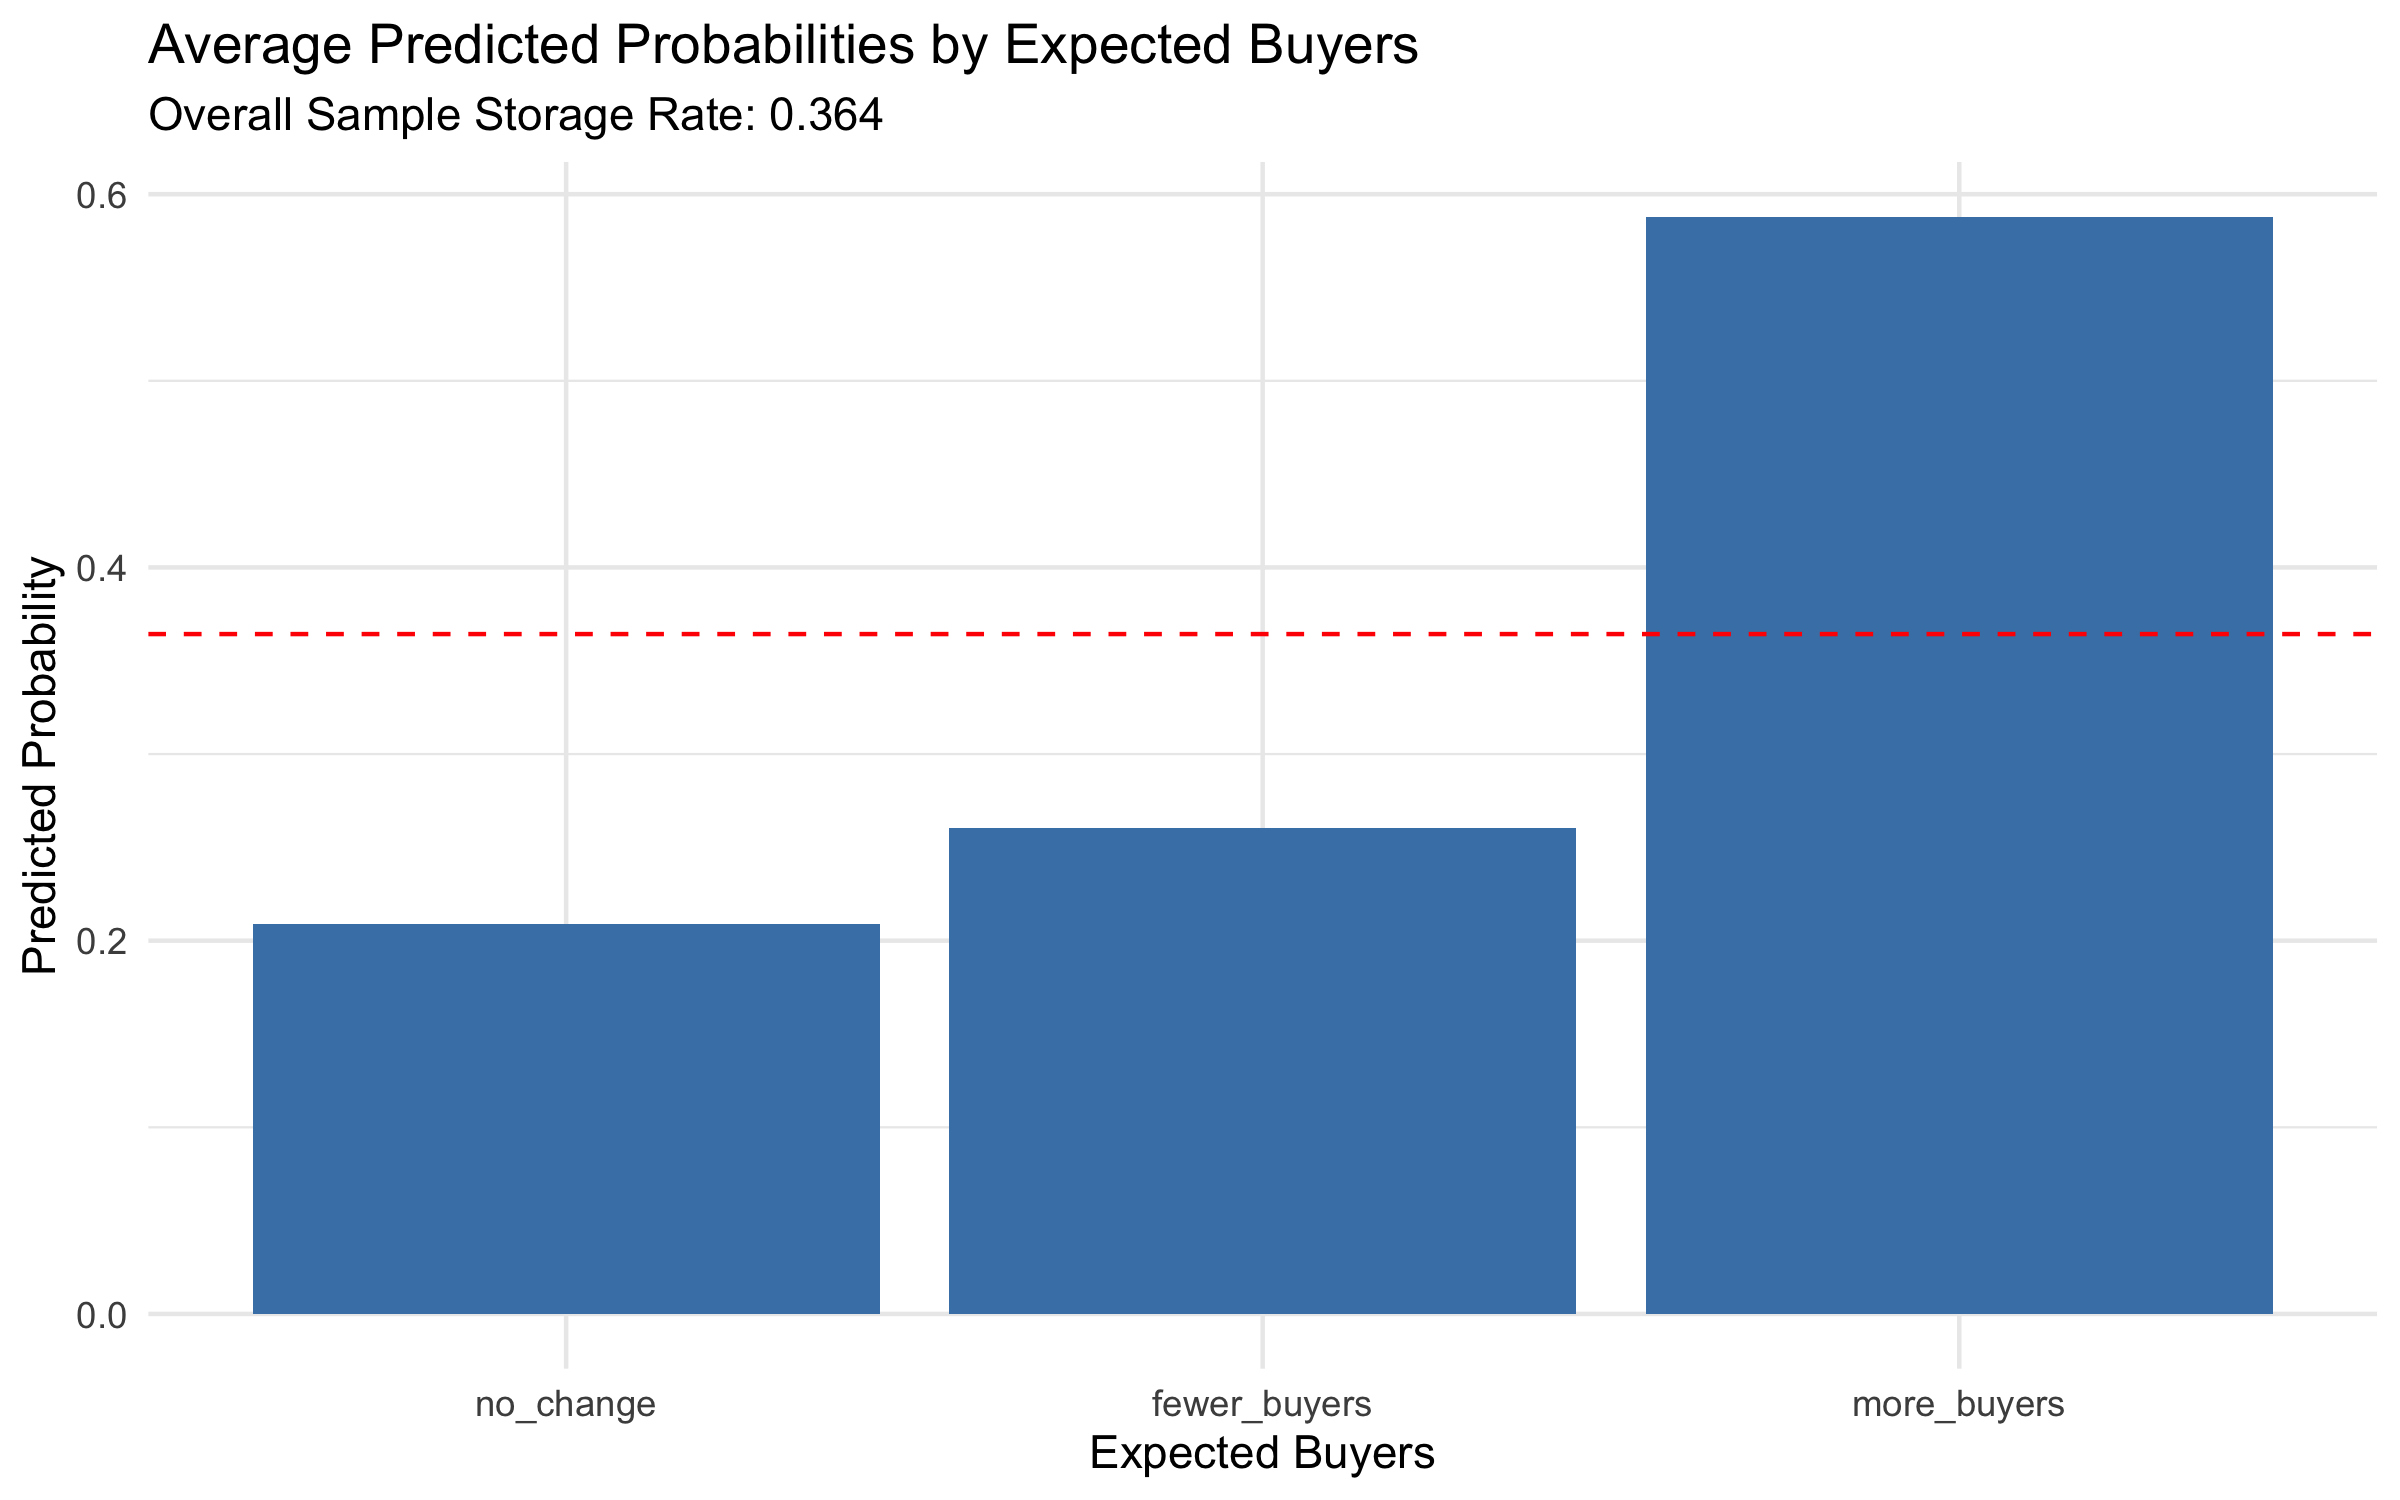
\includegraphics[height=0.28\textheight]{figures/overall_predicted_probs.png}
        \caption{}
    \end{subfigure}\\[2mm]
    
    \begin{subfigure}{\textwidth}
        \centering
        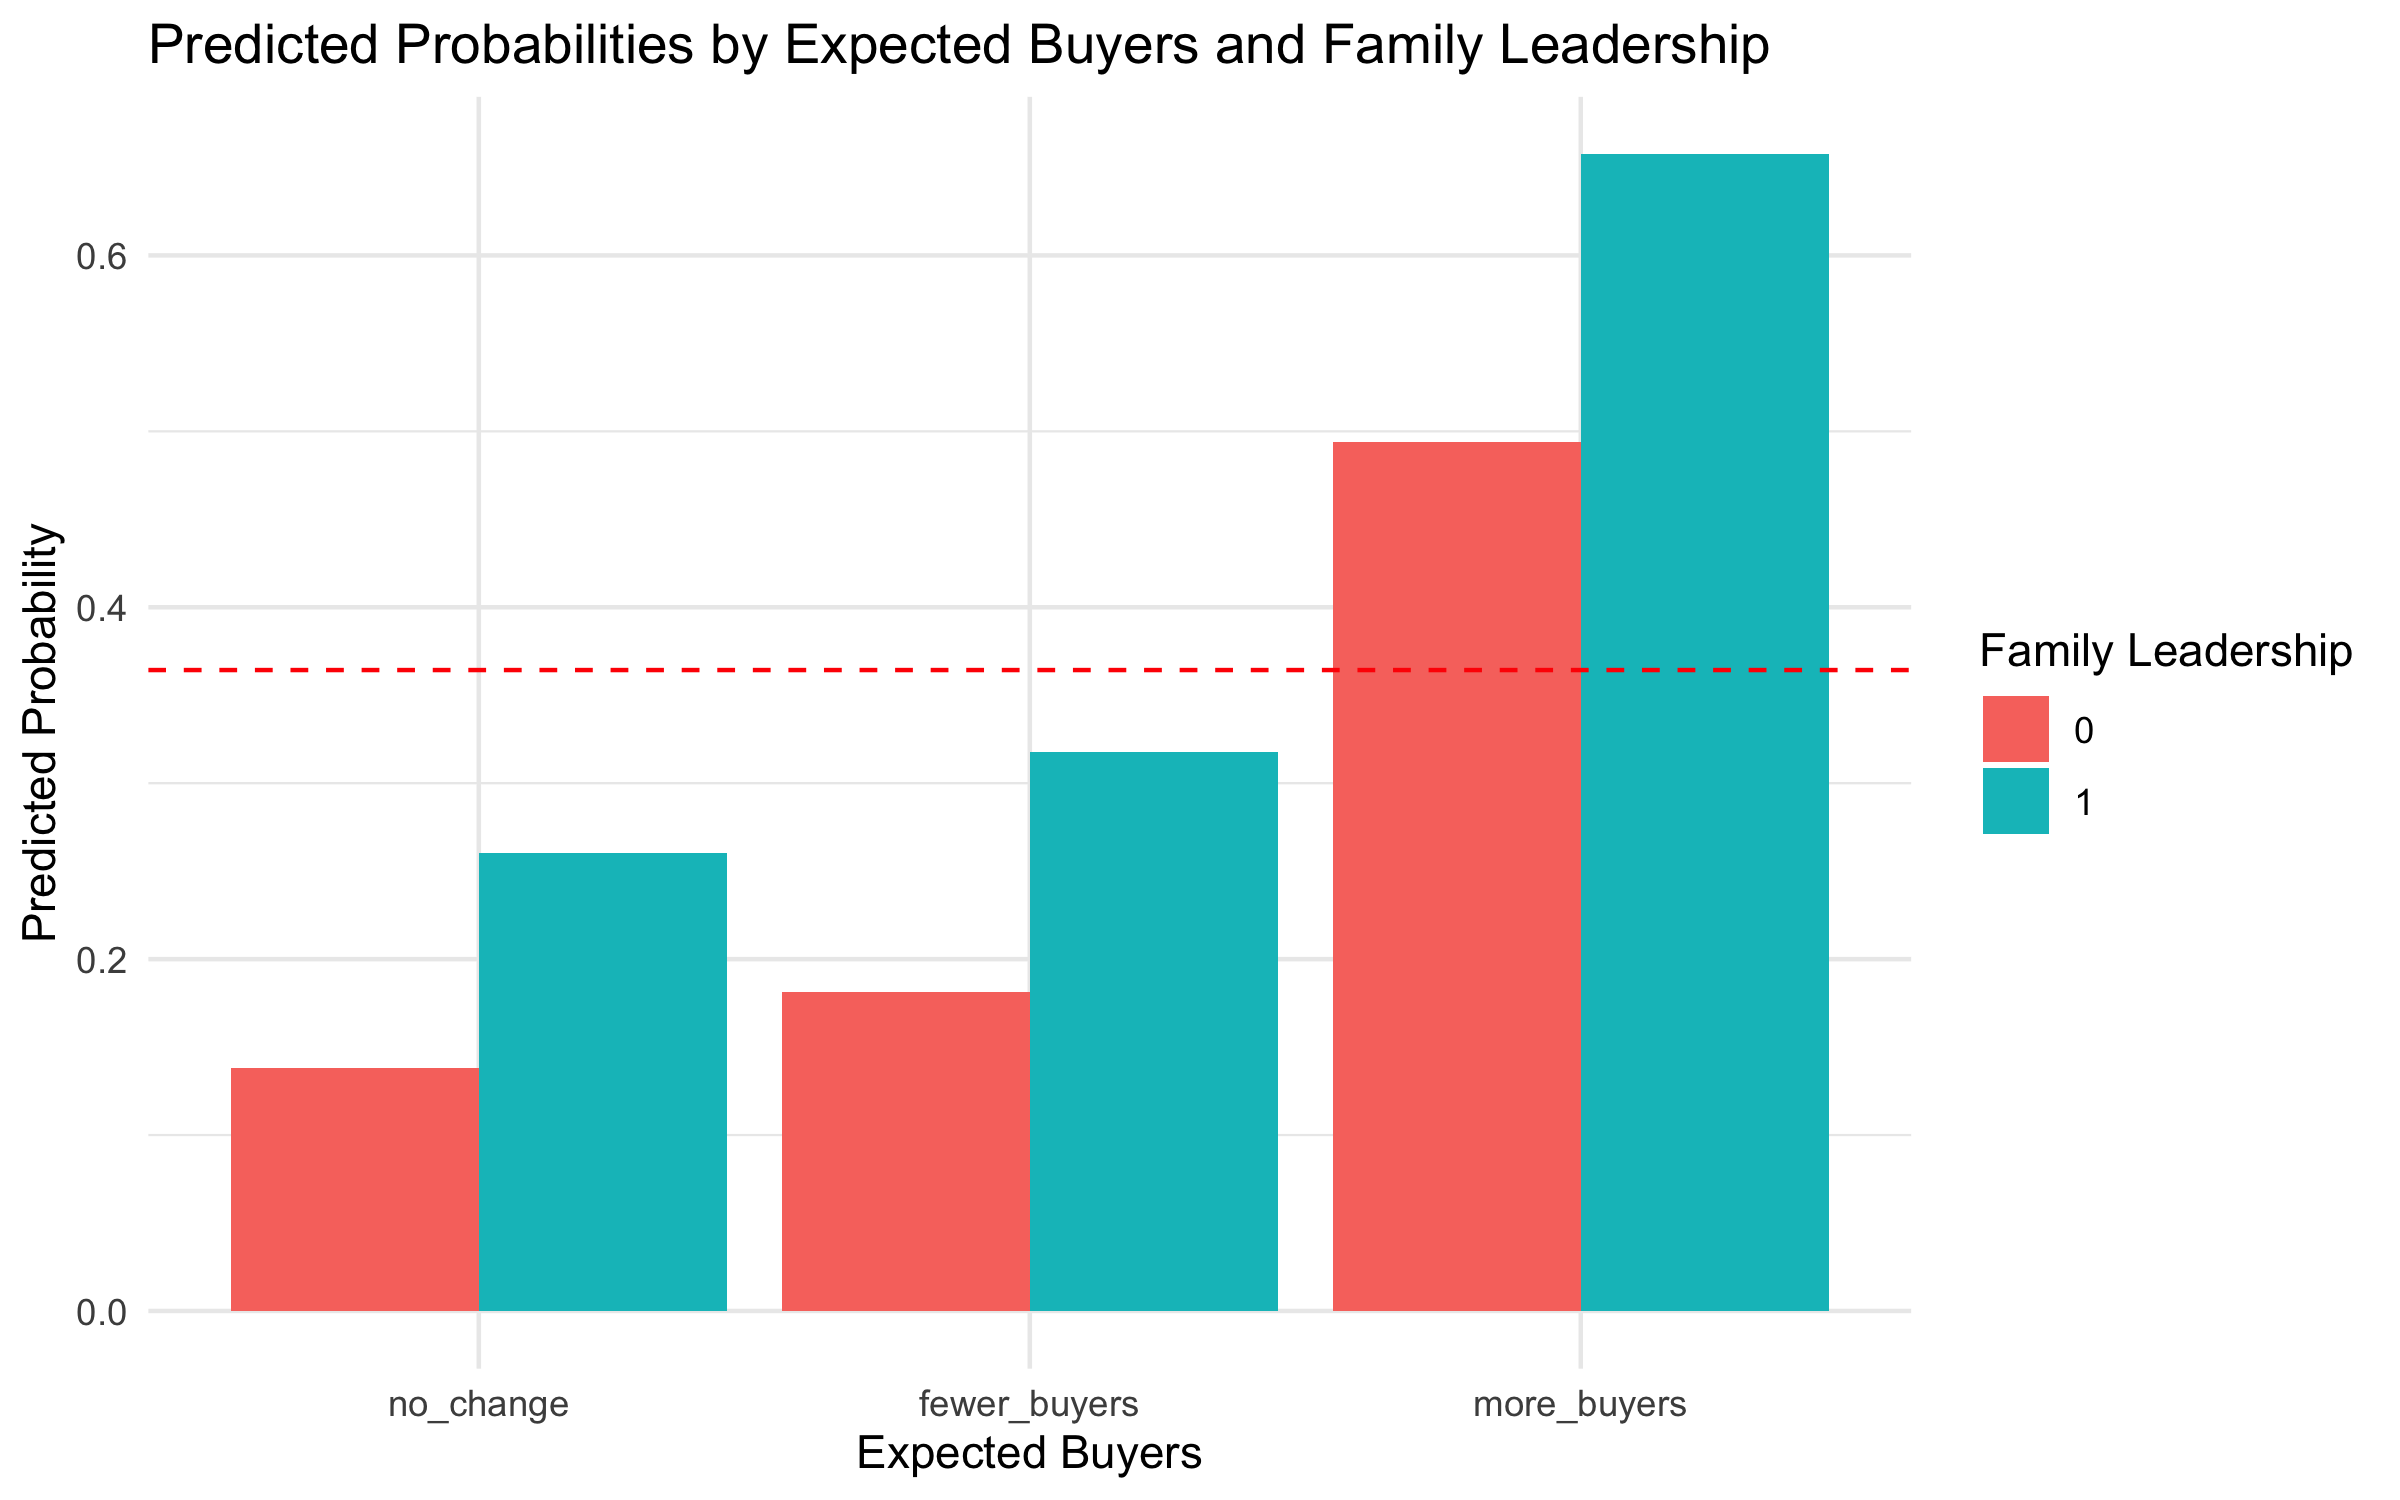
\includegraphics[height=0.28\textheight]{figures/predicted_probs_by_family.png}
        \caption{}
    \end{subfigure}\\[2mm]

    \begin{subfigure}{\textwidth}
        \centering
        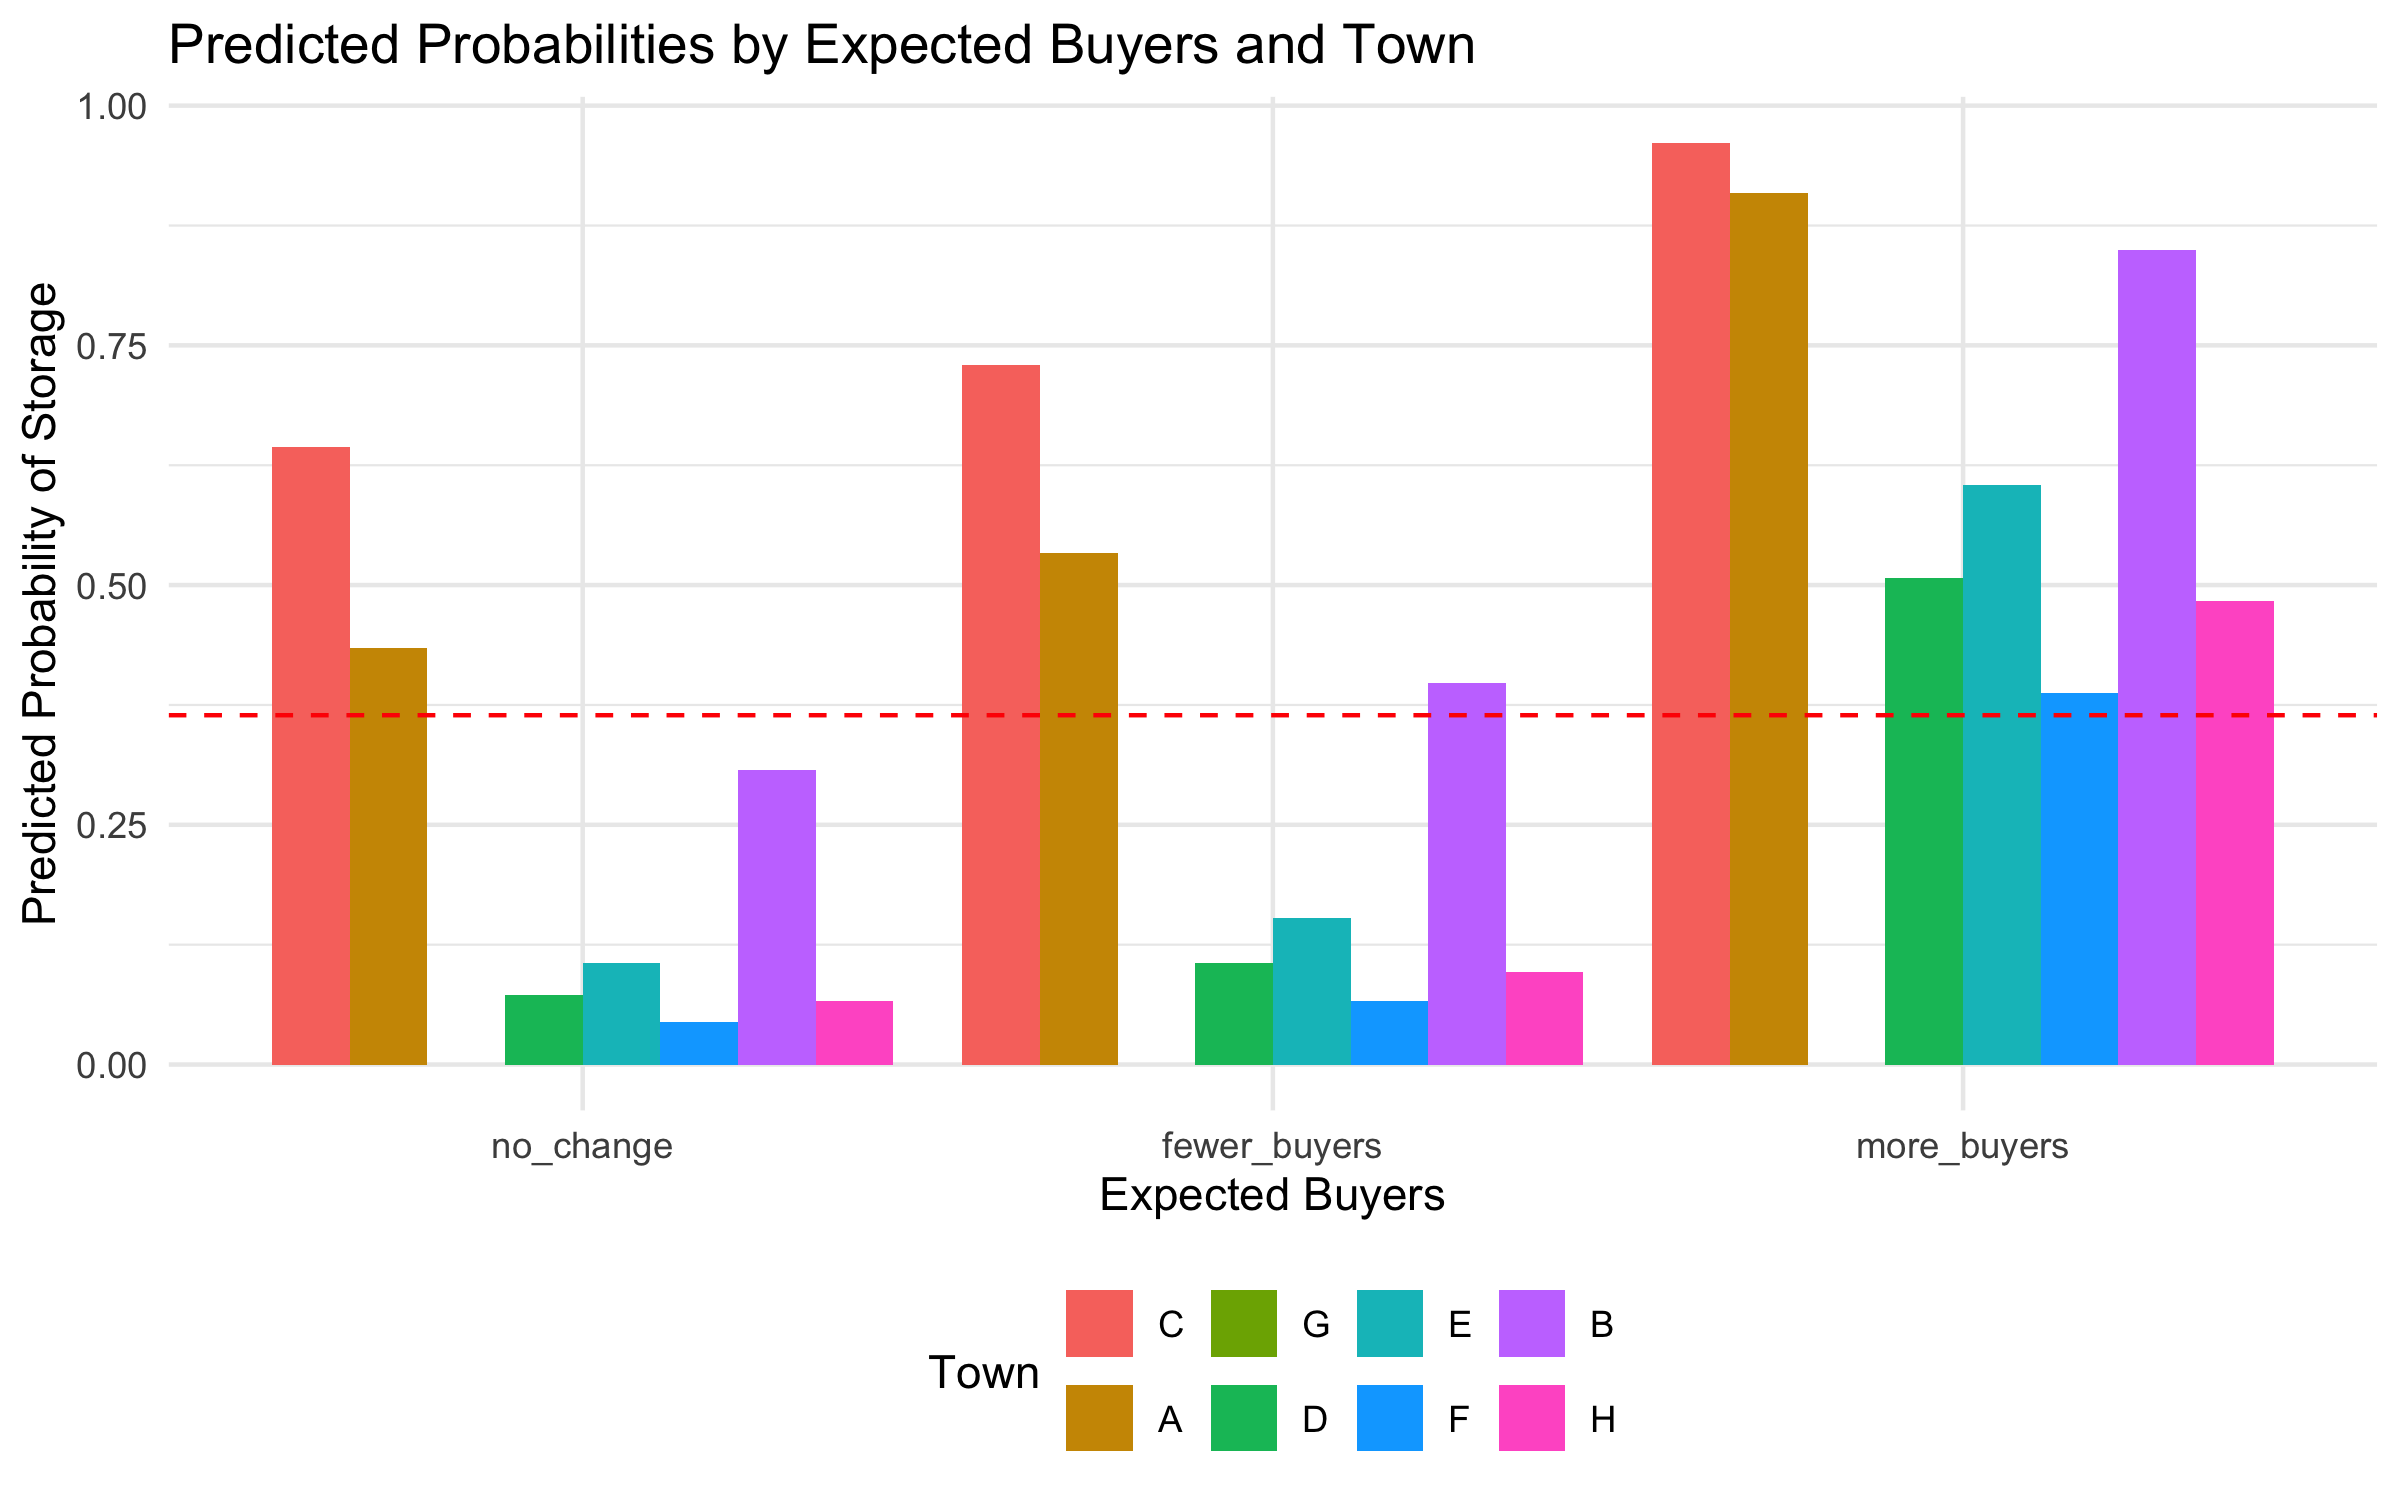
\includegraphics[height=0.28\textheight]{figures/predicted_probs_by_town.png}
        \caption{}
    \end{subfigure}


    \caption{Predicted Probabilities of Storage Usage by Expected Buyer Movement}
    \label{fig:three-images}
\end{figure}





\begin{figure}[ht]
    \centering
    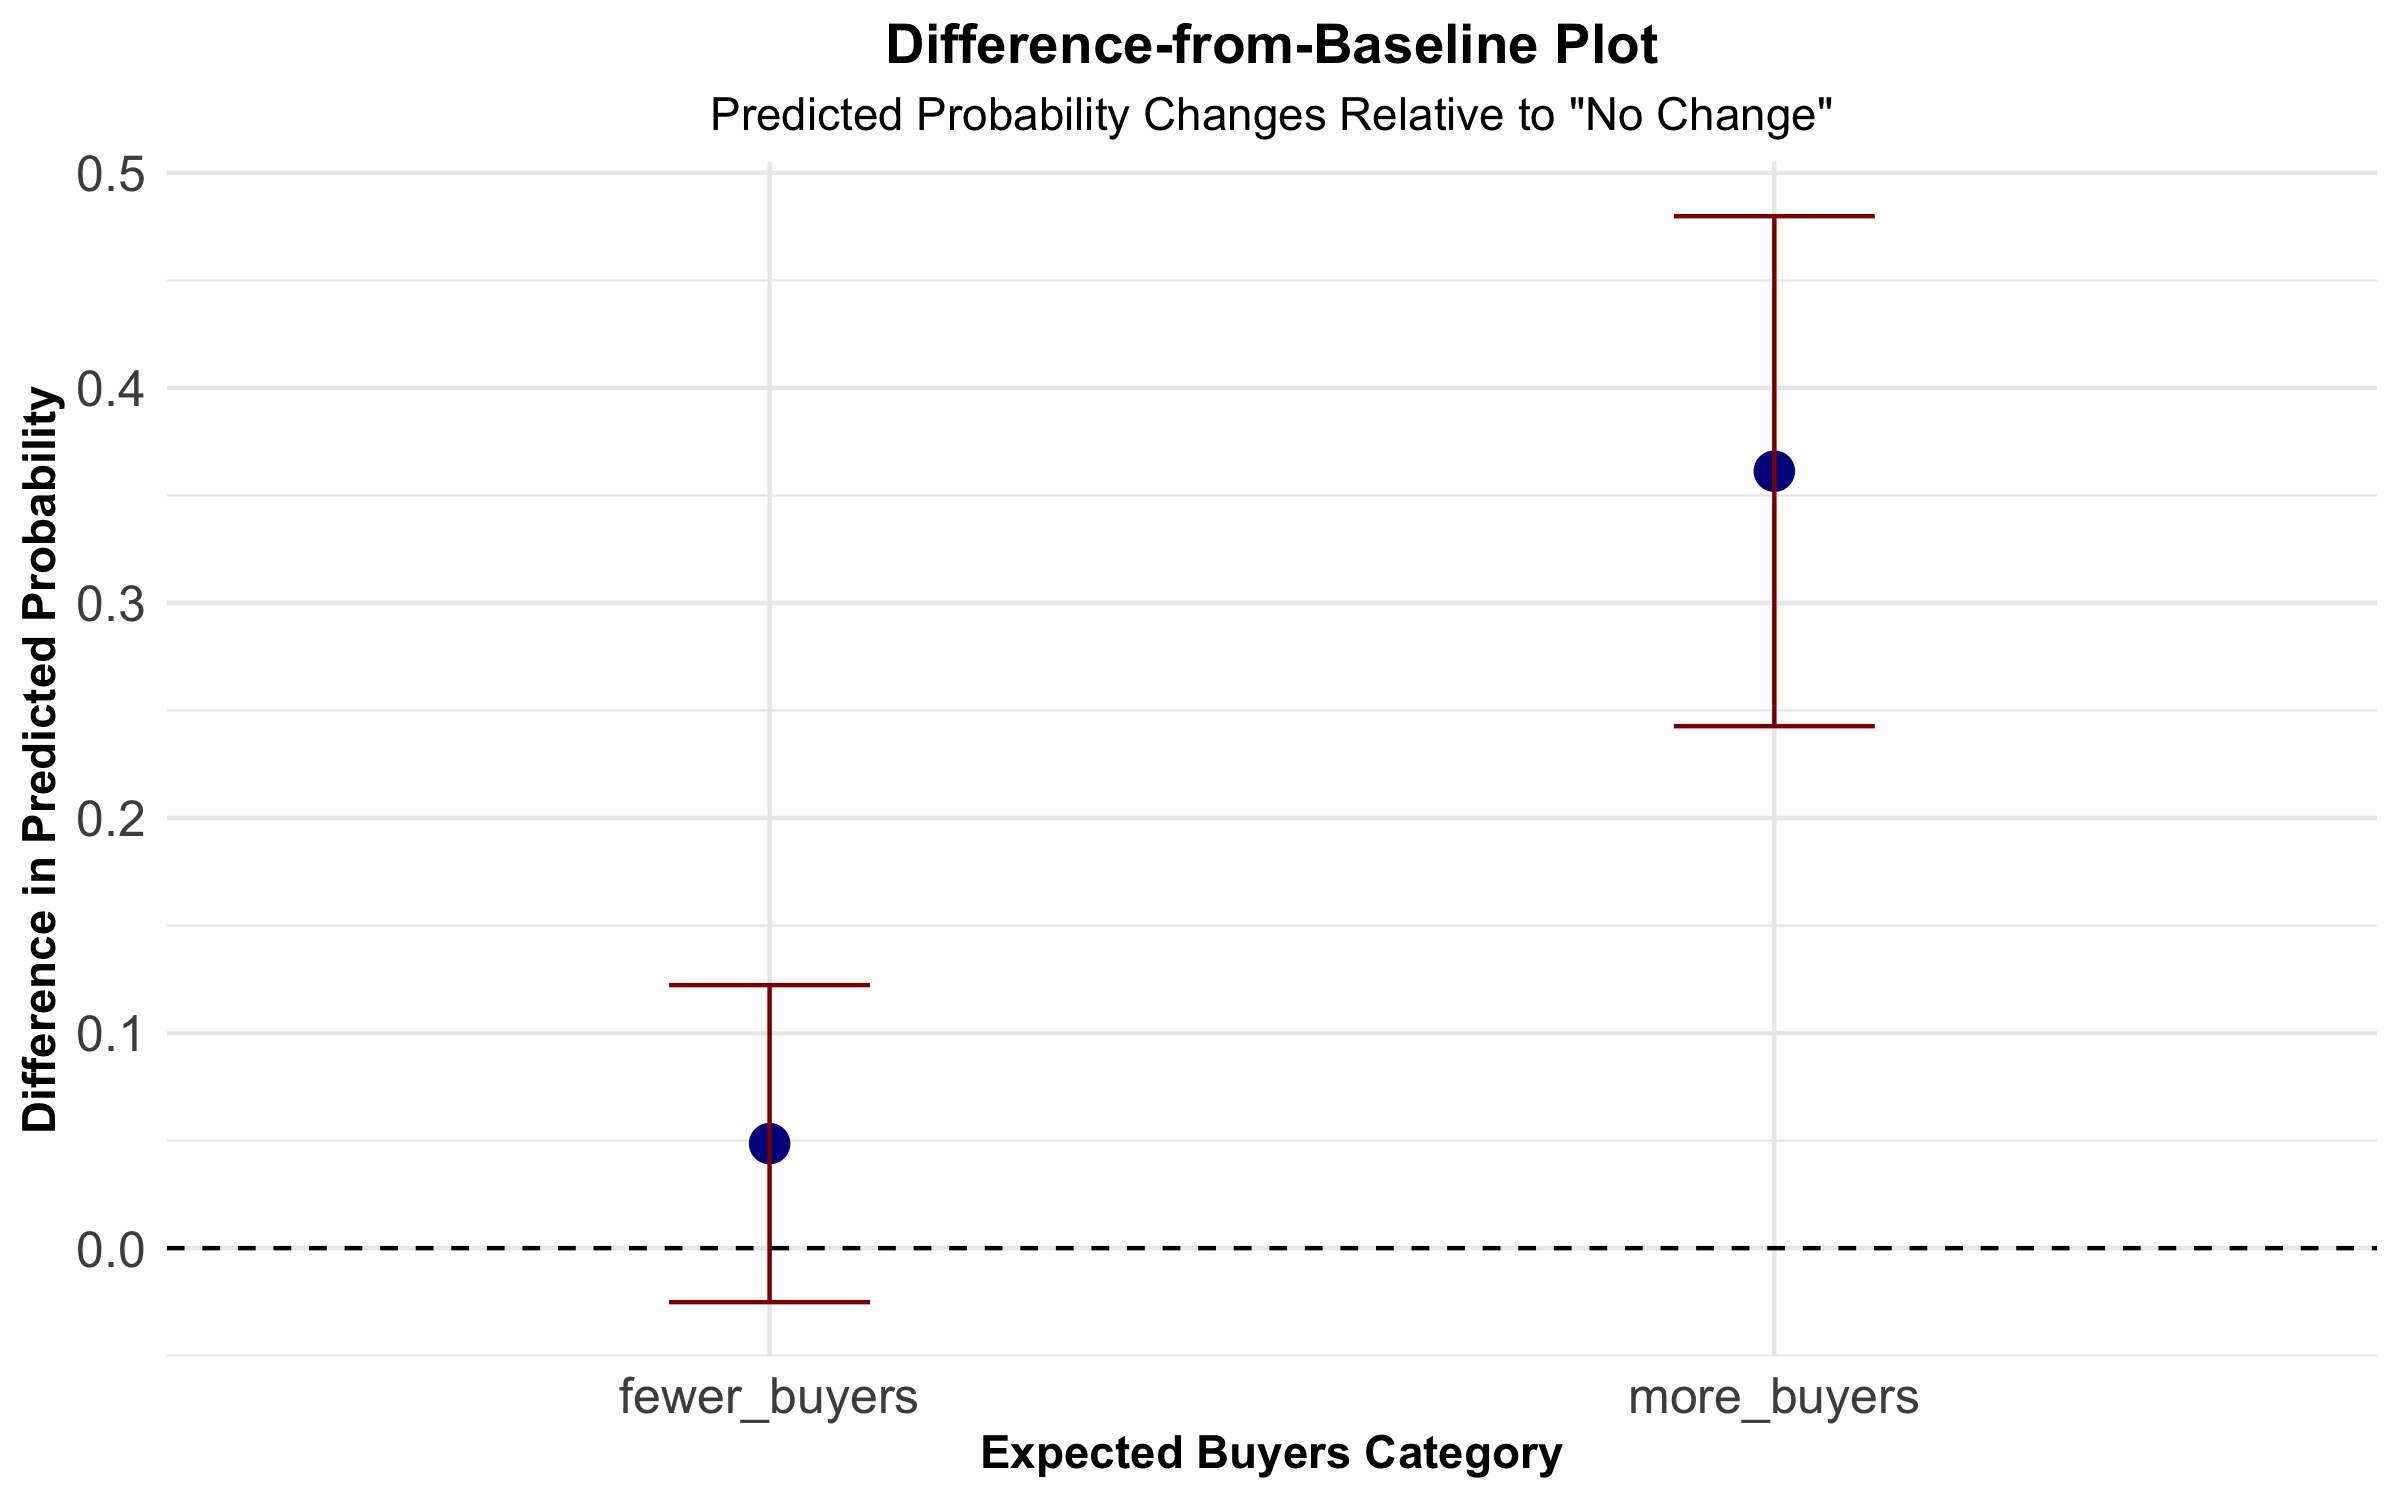
\includegraphics[width=1\textwidth]{figures/filtered_difference_from_baseline_plot.png}
    \caption{Difference-from-Baseline Plot}
    \label{Figure: Difference-from-Baseline Plot}
\end{figure}


\begin{figure}[ht]
\centering
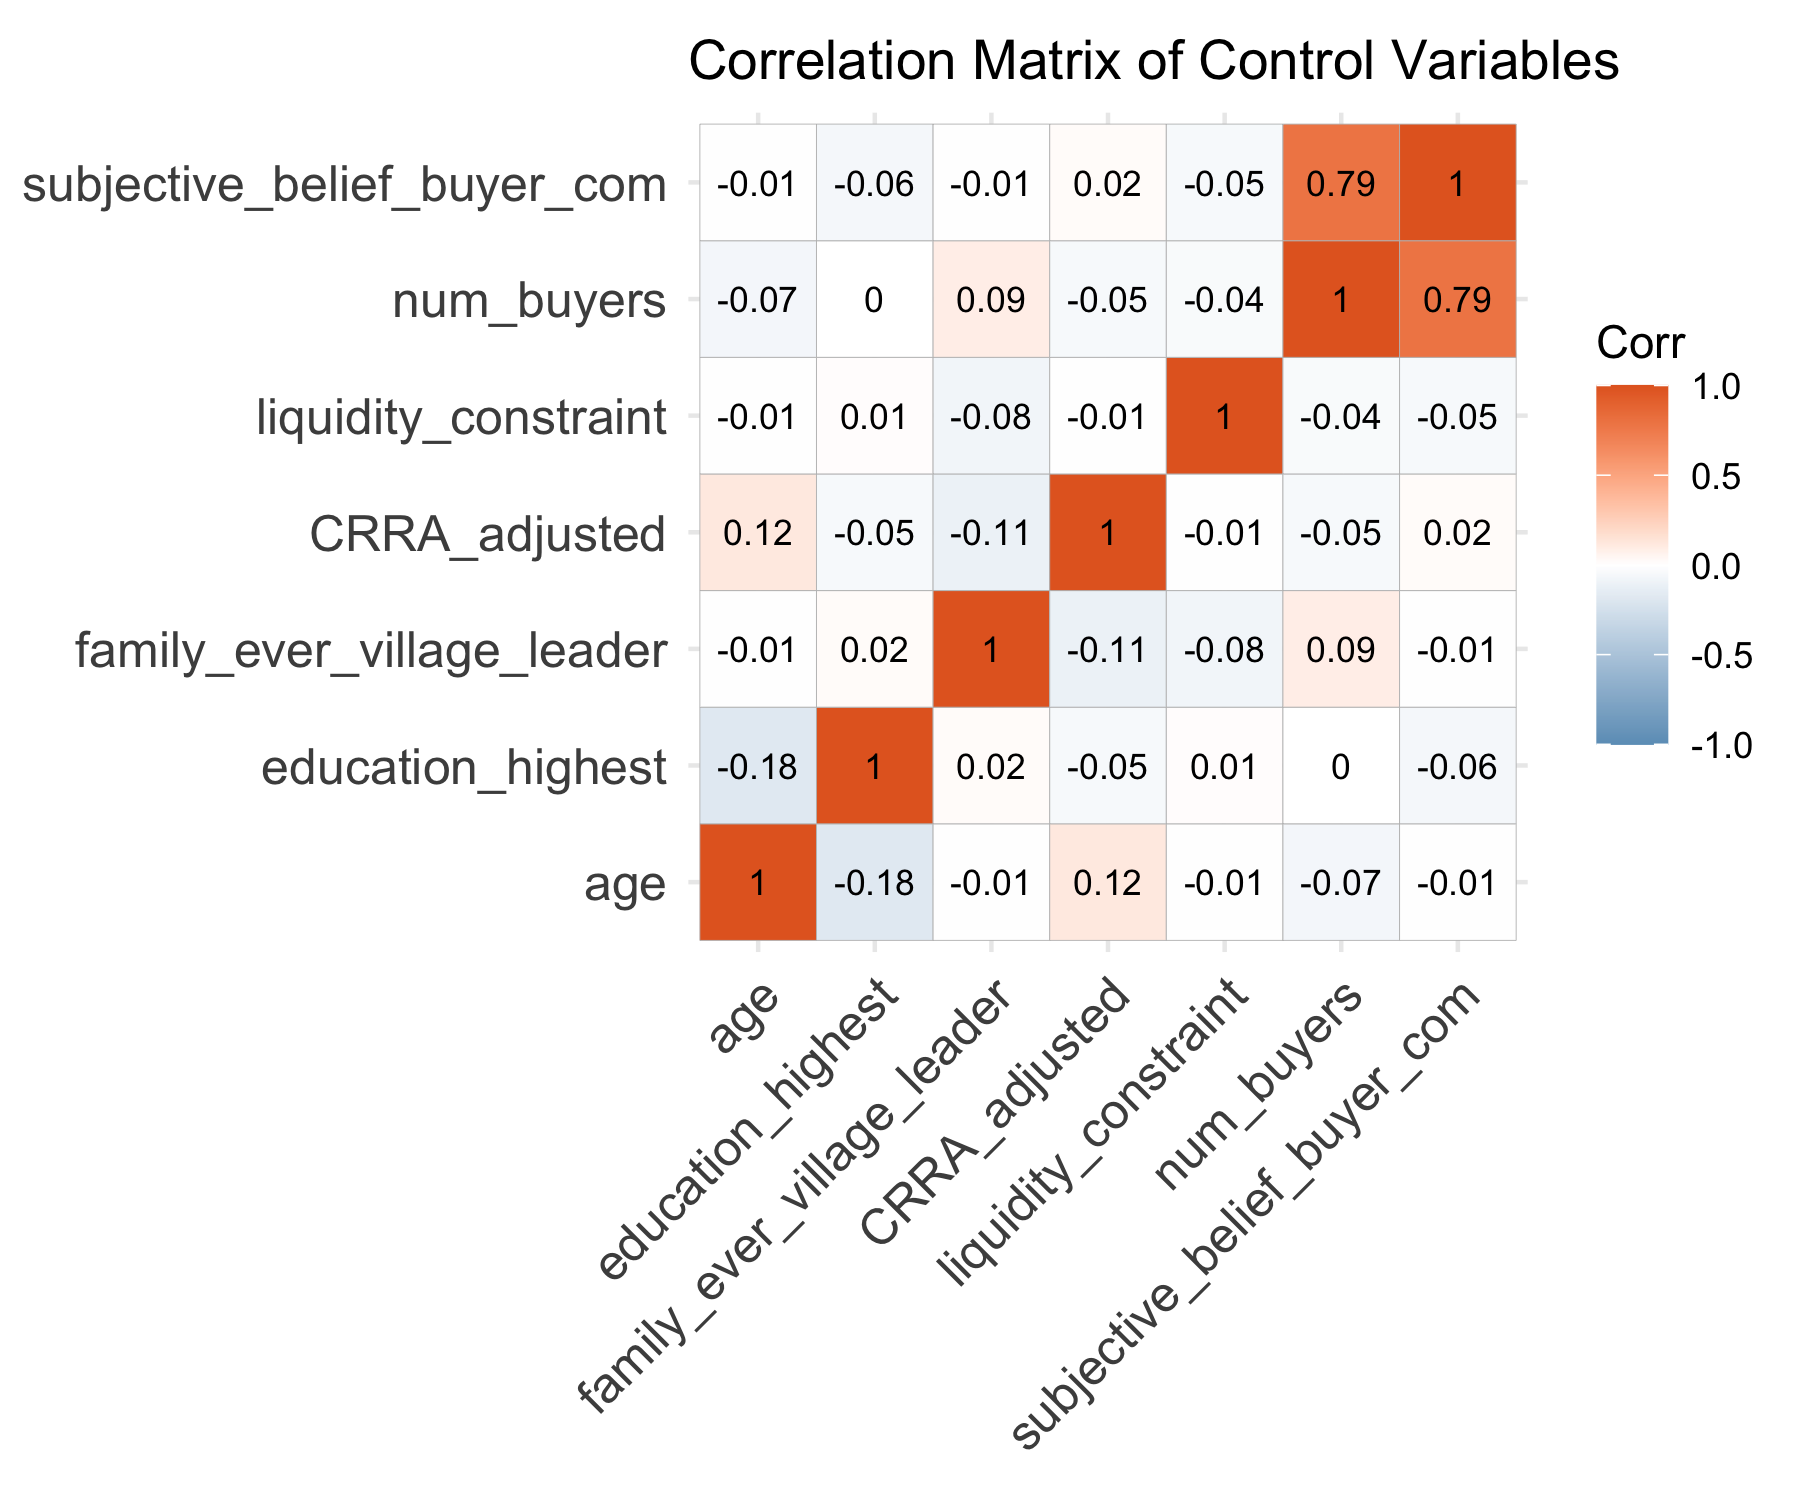
\includegraphics[width=1\textwidth]{figures/correlation_matrix_controls.png}
\caption{Correlation Matrix of Controls}
\label{Figure: Correlation Matrix of Controls}
\end{figure}

Demographic and risk-related factors continue to influence storage decisions in expected directions. Age has a consistently negative impact on storage usage, with AMEs of -0.003 (\(p < 0.1\)), indicating that older individuals are less likely to store their harvest. In contrast, family leadership status remains a strong positive predictor, with an AME of 0.105 (\(p < 0.01\)), suggesting that farmers with family leadership experience are significantly more likely to store their produce. Risk aversion also exerts a significant negative effect on storage decisions, with AMEs of -0.100 (\(p < 0.01\)), reinforcing the tendency of more risk-averse individuals to favor immediate sales over storage due to the uncertainty associated with future prices.

The correlation matrix of control variables, presented in Figure \ref{Figure: Correlation Matrix of Controls}, further contextualizes these findings by illustrating the relationships among key covariates. The negative correlation between age and education level (\(\rho = -0.18\)) is consistent with the observed effect of age on storage behavior, as younger farmers---who tend to have higher education levels---may be more receptive to market-based strategies, such as storage. Similarly, the relatively low correlation between risk aversion (CRRA adjusted) and other covariates suggests that its influence on storage decisions operates independently of other demographic characteristics. Additionally, farmers' subjective beliefs about buyer competition at harvest exhibit a strong positive correlation with the objective number of buyers at harvest (\(\rho = 0.79\)), reinforcing the idea that perceptions of market competition align closely with objective conditions, though they remain distinct factors. The overall low to moderate correlations among control variables reduce concerns about multicollinearity, supporting the reliability of the logistic regression estimates and their implications for storage behavior.



\subsection{Time to Sell: Expected Buyer Movement}

\subsubsection{Hazard Model with AFT}
\noindent 
To examine how farmers' expectations regarding buyer competition, price expectations, logistical factors, and external conditions influence the timing of their sales, I employ an accelerated failure-time (AFT) specification within a hazard model framework, following \cite{albuquerque2024market}. The AFT model is well-suited for analyzing interval-censored survival data, as it estimates the time until an event occurs---in this case, the sale of apples. This model assumes that covariates accelerate or decelerate the time to an event by a constant factor. A positive coefficient for a covariate indicates that it prolongs the time until the sale (delays selling), while a negative coefficient shortens it.

Given that my survey data only records the month of sale, an interval-censoring approach is used to improve the accuracy of selling duration estimates. The hazard model estimates the probability that a farmer sells apples at a given time, conditional on not having sold them earlier. In the AFT framework, the model is reinterpreted to focus on the speed of selling. The hazard rate for farmer \(f\) selling apples \(c\) at time \(t_{c,f}\) is given by:

\begin{equation}
    h_j(t_{c,f}) = h_0(t_{c,f}) \exp\left(-\mathbf{x}_{c,f} \boldsymbol{\beta}\right),
\end{equation}

where \(h_0(t)\) is the baseline hazard function, assumed to follow a Weibull distribution:

\begin{equation}
    h_0(t) = \alpha t^{\alpha-1}.
\end{equation}

The vector \(\mathbf{x}_{c,f}\) includes explanatory variables that influence the timing of sales. The survivor function \(S_j(t)\), which represents the probability that a farmer has not yet sold their apples by time \(t\), is related to the hazard function through:

\begin{equation}
    h_j(t) = -\frac{d \log S_j(t)}{dt}.
\end{equation}

For interval-censored data, the likelihood function is:

\begin{equation}
    \mathcal{L} = \prod_{j=1}^N \left(S_j(t_{i-1}) h(t_i)\right)^{y_{j,i-1}} S_j(t_{i-1})^{1-y_{j,i}},
\end{equation}

where \(y_{j,i} = 1\) if the sale occurs within the interval \(i\).

To control for unobserved location-specific factors such as weather conditions, road infrastructure, and market accessibility, township fixed effects are included in the empirical specification. This improves the model's ability to capture local heterogeneity, although it may reduce estimation efficiency due to the limited number of observations in some townships.


% Table created by stargazer v.5.2.3 by Marek Hlavac, Social Policy Institute. E-mail: marek.hlavac at gmail.com
% Date and time: Tue, Feb 25, 2025 - 17:56:36
\begin{table}[!htbp] \centering 
  \caption{Extended Weibull Survival Models with Controls} 
  \label{} 
\begin{tabular}{@{\extracolsep{5pt}}lcc} 
\\[-1.8ex]\hline 
\hline \\[-1.8ex] 
 & \multicolumn{2}{c}{\textit{Dependent variable:}} \\ 
\cline{2-3} 
\\[-1.8ex] & \multicolumn{2}{c}{Full Sample} \\ 
\\[-1.8ex] & (1) & (2)\\ 
\hline \\[-1.8ex] 
 More Buyers Future & 0.50$^{***}$ & 0.12 \\ 
  & (0.07) & (0.09) \\ 
  & & \\ 
 Less Buyers Future & $-$0.05 & $-$0.21$^{*}$ \\ 
  & (0.07) & (0.11) \\ 
  & & \\ 
 Family Village Leader & 0.05 & $-$0.06 \\ 
  & (0.08) & (0.10) \\ 
  & & \\ 
 Far to Small Storage & $-$0.30$^{***}$ & $-$0.14 \\ 
  & (0.07) & (0.10) \\ 
  & & \\ 
 Far to Large Storage & 0.01 & $-$0.13 \\ 
  & (0.10) & (0.15) \\ 
  & & \\ 
 Storage Purpose: Marketing & 0.33$^{***}$ & $-$0.11 \\ 
  & (0.06) & (0.14) \\ 
  & & \\ 
 Storage Purpose: Bargaining & 0.27$^{***}$ & $-$0.05 \\ 
  & (0.06) & (0.11) \\ 
  & & \\ 
 Education Level & 0.10$^{**}$ & 0.06 \\ 
  & (0.04) & (0.07) \\ 
  & & \\ 
 Number of Buyers & 0.03$^{**}$ & 0.04$^{*}$ \\ 
  & (0.01) & (0.02) \\ 
  & & \\ 
 Constant & 1.08$^{***}$ & 2.31$^{***}$ \\ 
  & (0.14) & (0.24) \\ 
  & & \\ 
\hline \\[-1.8ex] 
Town Fixed Effects & Yes & Yes \\ 
Observations & 549 & 200 \\ 
Log Likelihood & $-$527.73 & $-$283.46 \\ 
$\chi^{2}$ & 493.03$^{***}$ (df = 16) & 50.78$^{***}$ (df = 15) \\ 
\hline 
\hline \\[-1.8ex] 
\textit{Note:}  & \multicolumn{2}{r}{$^{*}$p$<$0.1; $^{**}$p$<$0.05; $^{***}$p$<$0.01} \\ 
\end{tabular} 
\end{table} 


\subsubsection{Results}
\noindent 
Table \ref{tab: extended Survival AFT with controls} presents the results from the AFT Weibull survival model, which estimates the duration (storing time) until farmers sell their apples. Column (1) includes the full sample, while Column (2) focuses exclusively on farmers who utilize storage.

\begin{enumerate}
    \item \textbf{Expected Buyer Competitiveness and Time to Sell:} Farmers' expectations about future buyer competition exhibit distinct effects on their marketing timing. In the full sample (Column 1), anticipating more buyers in the future significantly prolongs the time to sell (\(\beta = 0.50, p<0.01\)), suggesting that farmers expecting increased competition among buyers delay sales, likely in anticipation of higher farm-gate prices. This aligns with the theoretical expectation that greater buyer competition enhances farmers' bargaining power, incentivizing them to wait for more favorable market conditions.
    
    However, among storage users (Column 2), the coefficient on expecting more buyers is smaller and statistically insignificant (\(\beta = 0.12, p>0.1\)), indicating that for farmers already engaged in storage, expectations of further increased competition do not further delay their sales. This suggests that these farmers are already positioned to take advantage of higher prices and are less responsive to incremental changes in buyer expectations.

    Therefore, an optimistic projection on future market competitive conditions mainly encourages storage, but does not necessarily lead to a longer storage time (marketing wait).
    
    Conversely, expectations of fewer buyers in the future exhibit a negative but statistically insignificant coefficient in the full sample (\(\beta = -0.05, p>0.1\)), implying that pessimism about buyer competition does not significantly accelerate selling decisions across all farmers. Among storage users, however, expecting fewer buyers significantly shortens the time to sell (\(\beta = -0.21, p<0.1\)), suggesting that those who store their harvest are more sensitive to potential market downturns and may liquidate their stocks sooner when facing expectations of reduced competition.
    
    \item \textbf{Storage Conditions and Purpose:} 
    Logistical constraints related to storage access significantly influence the decision to store but have limited impact on the duration of storage. Specifically, greater distance to a storage facility reduces the likelihood of storage adoption but does not significantly affect the time apples are kept in storage, which is consistent with theoretical expectations. Farmers located farther from small storage facilities sell significantly earlier than those with closer access (\(\beta = -0.30, p<0.01\)), underscoring that distance imposes a meaningful transaction cost that limits farmers' ability to delay sales for better prices. In contrast, distance to large storage facilities does not have a statistically significant effect, suggesting that large storage infrastructures may be either less frequently utilized or more accessible under different institutional or market arrangements.
    
    The stated purpose of storage also plays a crucial role in determining the time to sell. Farmers who store with the explicit goal of marketing optimization exhibit significantly prolonged selling durations (\(\beta = 0.33, p<0.01\)), supporting the notion that these farmers strategically time their sales to capture better market conditions. Similarly, those who store for bargaining leverage also delay sales (\(\beta = 0.27, p<0.01\)), reinforcing the idea that farmers with stronger price negotiation motives tend to wait longer before selling. However, among storage users (Column 2), neither of these motivations significantly influences time to sell, likely because all individuals in this subsample are already engaged in storage, making other factors more decisive.
    
    \item \textbf{Human Capital and Market Conditions:} Farmers' education levels exhibit a significant and positive relationship with selling time in the full sample (\(\beta = 0.10, p<0.05\)), indicating that more educated farmers are more likely to delay sales, potentially due to better access to market information or stronger financial literacy. However, this effect diminishes among storage users (\(\beta = 0.06, p>0.1\)), suggesting that education primarily affects the initial decision to store rather than the subsequent timing of sales.
    
    The number of buyers at harvest in the market positively affects time to sell in both specifications, though the magnitude is relatively small. In the full sample, each additional buyer visiting during the harvest is associated with a slight delay in selling (\(\beta = 0.03, p<0.05\)), while among storage users, the effect is somewhat stronger (\(\beta = 0.04, p<0.1\)). This implies that market depth during harvest plays a role in prolonging sales, potentially by increasing farmers' confidence in their ability to obtain better prices.
\end{enumerate}

\subsubsection{Summary of Findings}
\noindent 
Overall, the results emphasize the critical role of farmers' expectations about future buyer competition in shaping marketing decisions. While higher expected buyer competition substantially delays sales, this effect is weaker among those who already engage in storage. Logistical constraints, particularly distance to storage, significantly accelerate sales in terms of the decision to store or not, highlighting the role of infrastructure in shaping market participation. Furthermore, farmers' stated storage motivations align with observed selling behavior, as those who store for marketing or bargaining purposes delay sales. Finally, human capital and local market depth exert additional influence, reinforcing the importance of education and buyer availability in determining optimal selling strategies.



\section{Conclusion}
\noindent This empirical analysis sheds light on the critical role of perceived and expected buyer competitiveness in shaping the storage and marketing decisions of smallholder farmers, using data from Fuji apple growers in Yanchang County, Central China. The key findings indicate that farmers' storage decisions are primarily driven by their subjective perceptions of buyer competition, rather than the actual number of buyers at harvest. This result is especially important in light of the existence of buyer collusion behavior that may undermine the apparent benefits of increased buyer presence. Farmers who perceive greater buyer competition at harvest are less likely to engage in storage, as they expect higher prices due to competitive market conditions. This highlights the importance of distinguishing between the observed number of buyers, which often fails to reflect true market competitiveness, and the expected number of buyers, which serves as a practical proxy for perceived competition in the farmers' minds.

In addition to harvest-time perceptions, farmers' expectations regarding future buyer competition significantly influence their storage decisions. Specifically, farmers are more likely to store their produce at harvest when they anticipate increased competition in the future, particularly over the next three months. This suggests that farmers view storage as a strategic tool to capitalize on expected market improvements. While the expectation of stronger competition incentivizes storage, expectations of fewer buyers do not significantly deter storage adoption. This asymmetry suggests that farmers are more responsive to the potential for price increases due to heightened competition than to the risks associated with reduced buyer presence. The findings underscore the role of perceived future market opportunities in shaping storage decisions, emphasizing the dynamic nature of smallholder decision-making in response to both current and anticipated market conditions.

The analysis further highlights the influence of demographic factors, risk preferences, and social capital on storage behavior. Specifically, older farmers and those with higher risk aversion are less likely to adopt storage, which is consistent with the theoretical expectation that more risk-averse individuals prefer immediate sales to mitigate uncertainty. Conversely, family leadership status and education level are positively associated with storage adoption. These factors suggest that farmers with stronger social networks and greater access to market information are more likely to invest in storage, recognizing its value for market timing and price negotiation. This finding indicates that access to storage is not only shaped by financial resources but also by social capital and education, which enhance farmers' ability to navigate market uncertainty and leverage storage as a marketing tool.

In line with these findings, the survival model analysis underscores the critical role of future buyer expectations in shaping marketing behavior. The expectation of increased buyer competition substantially delays sales, as farmers anticipate higher prices. However, this effect is weaker among those who already store their produce, indicating that farmers who are already engaged in storage are less responsive to additional market signals. This suggests that storage adoption provides a strategic buffer against market volatility, enabling farmers to hold out for more favorable prices without the immediate pressure to sell. Additionally, logistical constraints, particularly the distance to storage, significantly accelerate sales, highlighting how infrastructure access shapes market participation and sales timing. Farmers located farther from storage facilities are more likely to sell early, suggesting that the costs associated with storage access influence the timing of their sales. Furthermore, farmers who store for marketing optimization or bargaining leverage are more likely to delay sales, supporting the idea that storage decisions are not solely driven by financial necessity but by strategic considerations to maximize returns.

Lastly, human capital and local market depth exert additional influences on farmers' selling strategies. Education and buyer availability contribute to the farmers' ability to make more informed and market-efficient decisions, which, in turn, affects their storage and selling behaviors. More educated farmers, for instance, are more likely to delay sales, likely due to better access to market information and stronger financial literacy, which enables them to make informed decisions about when and how to sell. This underscores the broader economic forces at play, where access to education and market infrastructure plays a crucial role in shaping farmers' decision-making.




%----------------------------------------------------------------%
%----------------------------------------------------------------%

\newpage
\bibliography{reference.bib}

%--------------------------------------------------------%
\newpage
\appendix
\chapter{Mathematical Derivation}
    \section{Derivation of Farm Price under the FOOM Framework} \label{Appendix: Derivation of Farm Price under the FOOM Framework}

This appendix provides a rigorous derivation of the farm-gate price expression under the Flexible-Oligopoly-Oligopsony Model (FOOM), assuming perfect competition downstream and constant marginal cost.

\subsection{Model Setup}

Consider a market in which buyers procure a cash crop from farmers. Let \( p_f \) denote the farmgate price paid to farmers, \( p_r \) represent the downstream retail price, and \( c \) be the constant marginal cost incurred by buyers in marketing or processing. Buyers face an upward-sloping farm supply curve described by \( Q_f(p_f) \), characterized by price elasticity of farm supply \( \varepsilon \):

\begin{equation}
\varepsilon = \frac{p_f}{Q_f(p_f)} \frac{dQ_f}{dp_f}.
\end{equation}

Let \( \theta \geq 0 \) denote the oligopsony conduct parameter, capturing the degree of buyer market power, where \( \theta = 0 \) indicates perfect competition, and \( \theta = 1 \) indicates pure monopsony.

\subsection{Buyer's Optimization Problem}

Buyers maximize profits by selecting the quantity \( Q_f \) to purchase from farmers:

\begin{equation}
\max_{Q_f} \Pi = (p_r - c)Q_f - p_f(Q_f)Q_f.
\end{equation}


To obtain the optimal procurement quantity, we take the first derivative of the profit function \(\Pi\) with respect to the procurement quantity \(Q_f\):

\[
\frac{d\Pi}{dQ_f} = (p_r - c) - \frac{d}{dQ_f}\left[p_f(Q_f)Q_f\right].
\]

Applying the product rule, the derivative of the total procurement cost term \(p_f(Q_f)Q_f\) is:

\[
\frac{d}{dQ_f}\left[p_f(Q_f)Q_f\right] = p_f(Q_f) + Q_f \frac{dp_f(Q_f)}{dQ_f}.
\]

Thus, we have the first-order condition:

\[
\frac{d\Pi}{dQ_f} = (p_r - c) - \left[p_f(Q_f) + Q_f \frac{dp_f(Q_f)}{dQ_f}\right] = 0.
\]



To explicitly capture the degree of buyer market power (oligopsony), let's introduce the conduct parameter \(\theta\), which measures how much the buyer internalizes the impact of its procurement decision on the farmgate price \(p_f(Q_f)\):
\begin{itemize}
    \item \(\theta = 0\) indicates perfect competition (no market power).
    \item \(\theta = 1\) indicates pure monopsony (full internalization).
    \item Intermediate values \(0 < \theta < 1\) indicate oligopsony or partial market power.
\end{itemize}

Thus, the generalized first-order condition with market power becomes:

\[
(p_r - c) - p_f(Q_f) - \theta Q_f \frac{dp_f(Q_f)}{dQ_f} = 0.
\]

Therefore, rearranging this expression clearly, under oligopsony, the first-order condition incorporating buyer market power is:

\begin{equation}
p_r - c = p_f + \theta \frac{dp_f}{dQ_f}Q_f.
\end{equation}

This condition equates buyers' marginal revenue (net downstream price minus marketing cost) to their perceived marginal procurement cost, which includes the strategic effect of increased purchases on the farmgate price (see \cite{sexton2000industrialization}, \cite{rogers_rich_1994assessing}, or other FOOM models).

\subsection{Deriving the Farmgate Price Expression}

Expressing the derivative \( dp_f/dQ_f \) in terms of elasticity of supply \( \varepsilon \), we have:

\begin{equation}
\frac{dQ_f}{dp_f} = \varepsilon \frac{Q_f}{p_f} \quad \Rightarrow \quad \frac{dp_f}{dQ_f} = \frac{p_f}{\varepsilon Q_f}.
\end{equation}

Substituting this into the first-order condition gives:

\begin{equation}
p_r - c = p_f + \theta \left(\frac{p_f}{\varepsilon Q_f}\right)Q_f = p_f\left(1 + \frac{\theta}{\varepsilon}\right).
\end{equation}

Thus, we obtain the general FOOM pricing relation:

\begin{equation}
p_f = \frac{p_r - c}{1 + \frac{\theta}{\varepsilon}}.
\end{equation}

\subsection{Normalized Expression}

By normalizing the downstream net price \( p_r - c \) to unity, \( p_r - c = 1 \), the farmgate price simplifies neatly to:

\begin{equation}
p_f = \frac{\varepsilon}{\varepsilon + \theta}.
\end{equation}

\subsection{Economic Interpretation}

The resulting expression reveals intuitive insights:

\begin{itemize}
    \item Higher buyer market power \( \theta \) depresses the farmgate price \( p_f \).
    \item Greater elasticity of farm supply \( \varepsilon \) mitigates the downward pressure on the farm price caused by oligopsony power.
\end{itemize}


    \section{Comparative Statics Proof: Sign of Risk Aversion Effect} \label{Appendix: Proof of Sign of Risk Aversion Effect}

\begin{lemma}[Sign of Risk Aversion Effect with Net Price]
\label{lemma:sign-risk-aversion}
Suppose $\mathbb{E}_1[\Delta_\theta] \in [-\theta_1, 1-\theta_1]$, $\theta_1 \in [0,1]$, $\delta \in (0,1)$, and $c \in [0,1)$. Then, under these conditions, the partial derivative $\partial \log \kappa/\partial \gamma$ is negative:
\[
\frac{\partial \log \kappa}{\partial \gamma} < 0.
\]
\end{lemma}

\begin{proof}
Under proportional storage costs, the intertemporal return $\kappa$ becomes:
\[
\log \kappa = \frac{1}{\gamma} \log \delta + \frac{\gamma - 1}{\gamma} \left[ \log(1 - c) + \log\left(1 + \frac{\mathbb{E}_1[\Delta_\theta]}{1 + \theta_1} \right) \right].
\]
Taking the derivative with respect to $\gamma$:
\[
\frac{\partial \log \kappa}{\partial \gamma}
= \frac{1}{\gamma^2} \left[ -\log \delta + \log(1 - c) + \log\left(1 + \frac{\mathbb{E}_1[\Delta_\theta]}{1 + \theta_1} \right) \right].
\]

Note that:
\begin{itemize}
    \item $\log \delta < 0$ since $\delta \in (0,1)$;
    \item $\log(1 - c) < 0$ since $c \in (0,1)$;
    \item $\log\left(1 + \frac{\mathbb{E}_1[\Delta_\theta]}{1 + \theta_1} \right) \in (-0.693, 0.693)$, as before.
\end{itemize}

Together, $\log(1 - c) + \log\left(1 + \frac{\mathbb{E}_1[\Delta_\theta]}{1 + \theta_1} \right) < \log\left(1 + \frac{\mathbb{E}_1[\Delta_\theta]}{1 + \theta_1} \right) < |\log \delta|$ for most economically relevant calibrations.

Hence, the entire bracketed term is negative:
\[
-\log \delta + \log(1 - c) + \log\left(1 + \frac{\mathbb{E}_1[\Delta_\theta]}{1 + \theta_1} \right) < 0,
\]
which implies:
\[
\frac{\partial \log \kappa}{\partial \gamma} < 0.
\]

\medskip
\noindent
\textbf{Corner case:} If $\delta$ is extremely close to $1$, $c$ is very small, and $\mathbb{E}_1[\Delta_\theta]$ is strongly negative, it is theoretically possible for the total expression inside brackets to be positive. However, this is outside the range of typical empirical calibrations. Under normal economic settings, the result holds.
\end{proof}


    \section{Conceptual Framework: Linear Mean-Variance Approach} \label{Appendix: mean-variance approach}
\noindent In the main text, I model farmer storage decisions under market-structural uncertainty using a CRRA (constant relative risk aversion) utility specification, which is widely adopted in agricultural economics and allows for a structurally interpretable mapping between risk preferences and observed behavior. This choice facilitates empirical calibration, as the CRRA form nests intuitive behavioral responses and aligns well with micro-level data on consumption and risk. Crucially, it maintains coherence between the theoretical framework and the empirical analysis, which relies on price expectations and storage behavior inferred from actual market data. Since there is limited empirical guidance on how to calibrate abstract risk aversion coefficients across different agricultural contexts, preserving this consistency helps ensure that the model remains empirically grounded and interpretable.

Nonetheless, in the Appendix here, I provide an alternative formulation based on a mean–variance (MV) decision rule as a complement \citep{levy1979approximating, schoemaker1982expected}. The principal advantage of the MV framework is that it avoids assuming any specific utility function, thereby abstracting away from the functional form of farmers’ risk preferences \citep{coyle1992risk}. This allows for greater transparency in tracing how storage incentives respond to changes in price levels, volatility, and market structure. MV has been adopted in many works in the field of agricultural economics such as \cite{saitone2009optimal} and \cite{yu2018effects}. While my inter-temporal price rule formation from the \textit{FOOM} models (the expected second-period revenue is not an affine transformation of the stochastic buyer power change), hence the MV model is not always consistent with expected utility maximization \citep{meyer1987two}, a careful choice from a mean–variance efficient frontier will approximately maximize expected utility \citep{markowitz2014mean, chiu2016supply}.




\subsection{Economic Environment}
\noindent
A representative farmer harvests a normalized quantity of one unit at the beginning of period 1 and chooses a \textit{storage share} \(s\in[0,1]\). The farmer can (i) sell \((1-s)\) units immediately at the certain price \(p_{1}\), or (ii) store \(s\) units until period 2, incurring a proportional storage-cum-discount factor \(\delta\in(0,1]\). Future market conditions are summarized by an ex-ante random \textit{buyer-power index} \(\tilde\theta_{2}\). Conditional on \(\tilde\theta_{2}\), the second-period price is generated by the structural rule:
$$
\tilde p_{2} = \frac{1}{1+\tilde\theta_{2}}, \qquad 
\tilde\theta_{2} \sim (\mu_\theta, \sigma_\theta^{2}).
$$
Total discounted revenues are therefore:
$$
\pi(s) = (1-s)p_{1} + \delta s\,\tilde p_{2}.
$$

\subsection{Preference Representation}
\noindent
Departing from expected-utility maximization, I adopt the standard \textit{mean–variance} (two-moment) method, which is the quadratic approximation to any twice-differentiable utility around its certainty equivalent:
$$
\max_{s\in[0,1]}
\;\;{\cal V}(s)
\equiv
\mathbb E[\pi(s)]
-\frac{\kappa}{2}\operatorname{Var}[\pi(s)],
\quad\kappa>0.
$$
The parameter \(\kappa\) indexes the marginal rate of substitution between expected profit and profit risk; it maps one-to-one to the coefficient of (local) absolute risk aversion in the underlying utility function.

\subsection{Moments of Future Price (Delta Method)}
\noindent
Let $f(x)=1/(1+x)$. Evaluating at the mean $\mu_\theta$ and retaining terms up to second order:

$$
\begin{aligned}
\mathbb E[\tilde p_{2}]
&\approx f(\mu_\theta)+\tfrac12 f''(\mu_\theta)\,\sigma_\theta^{2}
= \frac{1}{1+\mu_\theta}
  +\frac{\sigma_\theta^{2}}{(1+\mu_\theta)^{3}},\\[6pt]
\operatorname{Var}[\tilde p_{2}]
&\approx\bigl[f'(\mu_\theta)\bigr]^{2}\sigma_\theta^{2}
= \frac{\sigma_\theta^{2}}{(1+\mu_\theta)^{4}}.
\end{aligned}
$$
Define:
$$
A \equiv \frac{1}{1+\mu_\theta} + \frac{\sigma_\theta^2}{(1+\mu_\theta)^3},\qquad
B \equiv \frac{\sigma_\theta^2}{(1+\mu_\theta)^4}.
$$

\subsection{Optimal Storage Choice}
\noindent
Plugging the moments into \({\cal V}(s)\),
$$
\mathbb E[\pi(s)]       =(1-s)p_{1}+\delta sA,
\qquad
\operatorname{Var}[\pi(s)]=\delta^{2}s^{2}B.
$$
First-order condition for an interior optimum (\(0<s<1\)):
$$
\frac{\partial{\cal V}}{\partial s}
= -p_{1}+\delta A - \kappa\delta^{2}sB = 0
\quad\Rightarrow\quad
s^{\star} = \frac{\delta A - p_1}{\kappa \delta^2 B}.
$$
Imposing feasibility yields the policy rule:
$$
s^{\star}_\text{M--V} = \min\left\{1,\;\max\left\{0,\,s^{\star}\right\}\right\}.
$$

\subsection{Comparative Statics}
\noindent
I now characterize how the optimal storage share \(s^{\star}\) responds to changes in each underlying parameter, focusing on marginal effects within the interior solution region. The closed-form expression
$$
s^{\star} = \frac{\delta A - p_1}{\kappa \delta^2 B},
\qquad
A = \frac{1}{1 + \mu_\theta} + \frac{\sigma_\theta^2}{(1 + \mu_\theta)^3},
\quad
B = \frac{\sigma_\theta^2}{(1 + \mu_\theta)^4},
$$
implies that signs and magnitudes of changes depend critically on how each parameter affects the numerator (expected gain from waiting) and the denominator (penalty for price risk).

\paragraph{Current spot price \(p_1\).}
Differentiating \(s^{\star}\) with respect to \(p_1\) yields:
$$
\frac{\partial s^{\star}}{\partial p_1} = -\frac{1}{\kappa \delta^2 B} < 0.
$$
This effect is linear and unambiguous: a higher harvest-season price reduces the attractiveness of waiting by increasing the opportunity cost of storage. Since the second-period price is uncertain, selling now at a known higher price becomes more appealing. The strength of this effect is attenuated by greater risk aversion \(\kappa\), higher variance \(B\), or greater storage discounting \(\delta^2\).

\paragraph{Discount/storage factor \(\delta\).}
The derivative with respect to \(\delta\) is:
$$
\frac{\partial s^{\star}}{\partial \delta}
=
\frac{A - 2p_1/\delta}{\kappa \delta B}
=
\frac{(2p_1/\delta) - A}{\kappa \delta^2 B}.
$$
The sign of this expression depends on the relative size of \(\delta A\) and \(2p_1\). If \(p_1 < \delta A / 2\), then \(\partial s^{\star}/\partial \delta > 0\), implying that a more favorable storage environment (e.g., through lower physical loss or discounting) increases the incentive to store. Conversely, when \(p_1\) is relatively high, further increases in \(\delta\) make variance penalties more salient (via the \(\delta^2\) term in the denominator), potentially decreasing storage.

\paragraph{Risk aversion \(\kappa\).}
Storage declines monotonically with risk aversion:
$$
\frac{\partial s^{\star}}{\partial \kappa}
=
-\frac{s^{\star}}{\kappa} < 0.
$$
A more risk-averse farmer places a higher penalty on variance and therefore chooses to market a larger share of the harvest at the safe, known price \(p_1\). The strength of this effect is proportional to the initial level of storage \(s^{\star}\) and inversely proportional to \(\kappa\) itself.

\paragraph{Mean buyer power \(\mu_\theta\).}
Changes in \(\mu_\theta\) influence both the expected price (\(A\)) and its variance (\(B\)). Applying the chain rule:
$$
\frac{\partial A}{\partial \mu_\theta} = -\frac{1}{(1 + \mu_\theta)^2} - \frac{3\sigma_\theta^2}{(1 + \mu_\theta)^4} < 0,\qquad
\frac{\partial B}{\partial \mu_\theta} = -\frac{4\sigma_\theta^2}{(1 + \mu_\theta)^5} < 0.
$$
An increase in the average level of buyer power lowers both the expected future price and its variance. However, the effect on \(s^{\star}\) is dominated by the decline in \(A\), which reduces the expected gain from deferring sales. Since the price variance \(B\) also falls, the risk-adjusted reward from waiting shrinks. Therefore:
$$
\frac{\partial s^{\star}}{\partial \mu_\theta} < 0,
$$
i.e., more monopsonistic market conditions on average lead farmers to store less.

\paragraph{Variance of buyer power \(\sigma_\theta^2\).}
This parameter enters both the numerator and denominator of \(s^{\star}\), yielding a nontrivial tradeoff between \textit{convexity gains} (via Jensen’s inequality) and \textit{risk penalties}. Substituting \(A = A_0 + C\sigma_\theta^2\), \(B = D\sigma_\theta^2\), with \(A_0 = 1/(1 + \mu_\theta)\), \(C = 1/(1 + \mu_\theta)^3\), and \(D = 1/(1 + \mu_\theta)^4\), the derivative becomes:
$$
\frac{\partial s^{\star}}{\partial \sigma_\theta^2}
=
\frac{\delta A_0 - p_1}{\kappa \delta^2 D \sigma_\theta^4}.
$$
Hence,
$$
\text{sign}\left( \frac{\partial s^{\star}}{\partial \sigma_\theta^2} \right)
= \text{sign}\left( \delta A_0 - p_1 \right).
$$
When the expected future price (without Jensen's correction) already exceeds the current price, increases in variance enhance expected revenues and encourage storage. Otherwise, the added risk dominates, and storage is reduced. This reflects a \textit{threshold property}: variance is beneficial only when the price gap \(\delta/(1 + \mu_\theta) - p_1\) is positive.

\paragraph{Summary Table: Signs of Marginal Effects on Interior Storage Share \(s^{\star}\)}

\begin{table}[H]
\centering
\begin{tabular}{llll}
\toprule
\textbf{Parameter} & \(\partial s^{\star}/\partial(\cdot)\) & \textbf{Direction} & \textbf{Mechanism} \\
\midrule
\(p_1\) & \(< 0\) & \(\downarrow\) & Higher current price discourages storage \\
\(\delta\) & Mixed & \(\uparrow\) if \(\delta A > 2p_1\) & Storage gain vs. variance amplification \\
\(\kappa\) & \(< 0\) & \(\downarrow\) & More risk aversion → earlier selling \\
\(\mu_\theta\) & \(< 0\) & \(\downarrow\) & More monopsony power depresses future price \\
\(\sigma_\theta^2\) & \(\text{sign}(\delta/(1+\mu_\theta) - p_1)\) & \(\uparrow\) or \(\downarrow\) & Jensen gain vs. added risk \\
\bottomrule
\end{tabular}
\end{table}

These results highlight that while some comparative statics are globally monotonic, others depend on \textit{threshold conditions} shaped by the relative price gap between harvest and storage seasons.




\chapter{Further Discussions}
    %------------------------------------------------------%
\section{Time-Varying Competition Estimation}
\noindent To quantitatively evaluate the competitiveness of the oligopsonistic market faced by farmers, the study will employ an adapted version of the Lerner Index, denoted by $H$ as follows:
\begin{equation}
    H = \frac{E_t(P^w_{t+1}) - MC_t - P_t^f - S_{t,t+1}^w}{E_t(P^w_{t+1})}
\end{equation}
where $P^w_{t+1}$ captures the wholesaling price of downstream sales in month $t+1$ reported by intermediaries, $P_t^f$ represents the farm-gate price reported by farmers after the harvest in month $t$, $S_{t,t+1}^w$ shows the trader's storage cost from period $t$ to $t+1$, and $MC_t$ depicts the sum of other marginal costs of traders. In other words, the index captures the ratio of the trader's mark-up and their downstream selling price. 

The modified Lerner index could be also regarded as the pass-through of marginal product into the farm-gate price as the primary proxy for buyer's power, like in the approaches used by \cite{bergquist_dinerstein_2020} and \cite{atkin2015s}. The closer this ratio is to zero, $H \rightarrow 0$, the more competitive the oligopsonistic markets are perceived to be.

While our modified Lerner index offers a succinct measure of monopsony power, its practical application is limited due to challenges in accurately measuring traders' costs. However, since the inter-temporal behavior of prices and costs is our main focus, the delta of the Lerner Index should be reliable when we have a consistent series of traders' operational costs and storage expenses. 

To collect traders' marginal cost data and to control for demand shocks and variability, I will conduct another round of surveys on traders. The survey will include their operational costs and trading volume, and inquire about the existence of significant market events throughout the supply chain, such as fluctuations in market demand and changes in consumer preferences, natural disasters, or export/import markets.


%------------------------------------------------------%
\section{Extended Marketing Opportunities}
\noindent The adoption of cold storage has greatly extended the marketing opportunities of farmers in terms of both timing and channels. The sample of 549 households has confirmed that cold storage could greatly improve the bargaining power of farmers and boost their expected income through two primary channels:
\begin{itemize}
    \item \textbf{Better Sales Timing}: Cold storage enables farmers to store their harvest and sell at higher prices during the extended selling period. Farmers who do not use cold storage sell all their apples within one month of harvesting, while farmers who use cold storage can choose the optimal time to sell until June of the following year, allowing for a complete sales cycle lasting up to eight months. The result of my surveys shows that farm-gate prices during the first one or two months after harvest tend to be lower throughout the farming year due to the significant instantaneous supply. However, it remains unclear whether the higher farm-gate prices observed during the first post-harvest period reflect a monopsony market environment, which needs further exploration.
    
    \item \textbf{More Sales Channels}: The adoption of cold storage has expanded farmers' sales channels. It allows them to sell their harvest not only to the traders who frequently visit in late October or November and offer lower prices (ranging from 4 to 9 yuan/kg), but also to consumers through E-commerce platforms like WeChat and Taobao, where they can ask for higher prices (ranging from 10 to 14 yuan/kg). Consequently, the use of cold storage empowers apple growers to decide whether to sell in bulk or retail, depending on prevailing market conditions.
\end{itemize}


%------------------------------------------------------%
\section{Low Storage Adoption}
\noindent The adoption of cold storage among apple growers remains low. Although most of our survey respondents have the option to either rent large cold storage or build their small-scale storage, more than 85\% of them choose not to do so for the following reasons:
\begin{itemize}
    \item \textbf{Unbalanced Scale of Cold Storage}: Most of the available collective cold storage facilities are too large (over 100 tons), resulting in a low individual harvest-to-storage-volume (HSV) ratio, which leads to high costs for cold storage adoption. The storage capacity of cold storage in many villages and towns is excessively large, often hundreds or thousands of tons. To utilize cold storage, many farmers need to store their produce collectively, a decision-making process that is difficult to scale in the village, resulting in underutilized cold storage facilities. 
    
    However, I found that small cold storage units (approximately 20 to 40 tons) built by villagers have a higher utilization rate. Farmers only need to store their own harvest, without having to cooperate with others. As soon as one household in the village benefits from selling at a higher price, many other farmers follow suit, creating a positive effect. Nevertheless, due to low output, most individual apple farmers cannot fully leverage the advantages of cold storage capacity, which leads to doubts about the feasibility and cost-effectiveness of investing in cold storage.

    \item \textbf{High Transportation Loss and Cost of Usage}: When the cold storage is far from the apple orchard, transportation in the mountainous terrain becomes inconvenient, resulting in significant transportation losses. Additionally, the cost of using cold storage is relatively high. Renting either collective cold storage or storage owned by others in the village incurs storage fees ranging from 0.20 to 0.40 yuan per kilogram, regardless of the duration of storage. Considering that the price of apples per kilogram has fluctuated between 2.5 and 4.5 in recent years, the cost of using cold storage is not insignificant. In contrast, when using small self-built cold storage (with a capacity of 20 tons), the maintenance cost ranges from 250 to 350 yuan per month.
    
    If a farmer's annual apple output is 10,000 kilograms and they need to store them for three months to secure a higher price offer, the cost of renting cold storage would range from 2,000 to 4,000 yuan, while the maintenance fee for their storage would range from 750 to 1,050 yuan. The former is two to three times higher than the latter.

    \item \textbf{High Construction Investment}: The total cost of a self-built small cold storage with a 20-ton capacity is approximately 90,000 yuan, with government subsidies ranging from 40,000 to 50,000 yuan. However, some farmers are burdened with debts and cannot afford to invest more than 40,000 yuan in construction.

    \item \textbf{Risk Aversion}: To convert harvested fruits into profits quickly, many extreme risk-averse farmers opt to sell their produce at lower prices early in the season to reduce uncertainty, rather than relying on cold storage and future market conditions. During the harvest season in October, many fruit dealers enter rural areas to make direct purchases. Among farmers, obtaining income directly during the harvest season is often considered the most straightforward approach. It's worth noting that among the surveyed farmers, those with higher levels of education tend to delay selling apples, which aligns with cold storage ownership and risk preferences.
\end{itemize}

However, at the same time, Yanchang is still experiencing a shortage in the supply of storage facilities. Cold storage facilities across the county are consistently full each year. In other words, the overall storage capacity currently falls short of demand. Consequently, rental storage fees have increased from 0.4 yuan/kg last year to 0.5 yuan/kg this year. The inventory of large merchants' cold storage is complex, with about 50\% being the owners' own apples, and the remaining apples are mostly from small fruit merchants and farmers stored in their facilities.

In summary, the impact of cold storage adoption on farmers' welfare is closely related to the storage's "relative" capacity, i.e., the harvest-to-storage-volume (HSV) ratio. If apple production is sufficiently large to fill the entire cold storage, utilization rates are high, and farmers can choose to store their harvests with confidence, anticipating higher prices at the end of the year or even during the Spring Festival. In such cases, cold storage adoption tends to benefit farmers the most.

Conversely, when apple production is low compared to the cold storage scale, cold storage is more likely to be abandoned. Farmers believe that the profits from later sales may not cover the sunk costs, communication expenses, and losses associated with using cold storage and transporting apples. Consequently, they are more inclined to sell their produce promptly during the harvest season. However, our on-site survey indicates that farmers with access to cold storage have better bargaining power than those who do not. In this scenario, access to storage serves as a deterrent rather than being used actively, as traders often possess better storage facilities than farmers. Storage is not primarily used to preserve products but rather as a signal or implicit threat to compel traders to offer more competitive prices.
    \section{Important Notes}
\begin{enumerate}
    \item \textbf{Cartel Solution:} Cartel solution is NOT an NE for any static game, but it may be NE behavior in any single play of an infinite-horizon repeated game. (by Folk Theorem)
    
    \item \textbf{Why Cournot, instead of Bertrand?} Analogy to \cite{kreps1983quantity}, I can infer that when traders simultaneously and independently receive "downstream orders" for subsequent distribution, and I assume that the capacity level (the quantity of the downstream orders) are public information and traders compete in Bertrand-like price competition, with the supply allocated in Bertrand fashion where the provision that one cannot satisfy more supply than one's order from downstream in the first stage: \\
    "Capacity introduced + Bertrand" $\Longleftrightarrow$ "Cournot".

    \item \textbf{Supply Elasticity:} the village supply to this model should be elastic in both periods, but differ in two periods because farmers have the "outside" selling options differently. 
\end{enumerate}



\chapter{Fieldwork Surveys}
    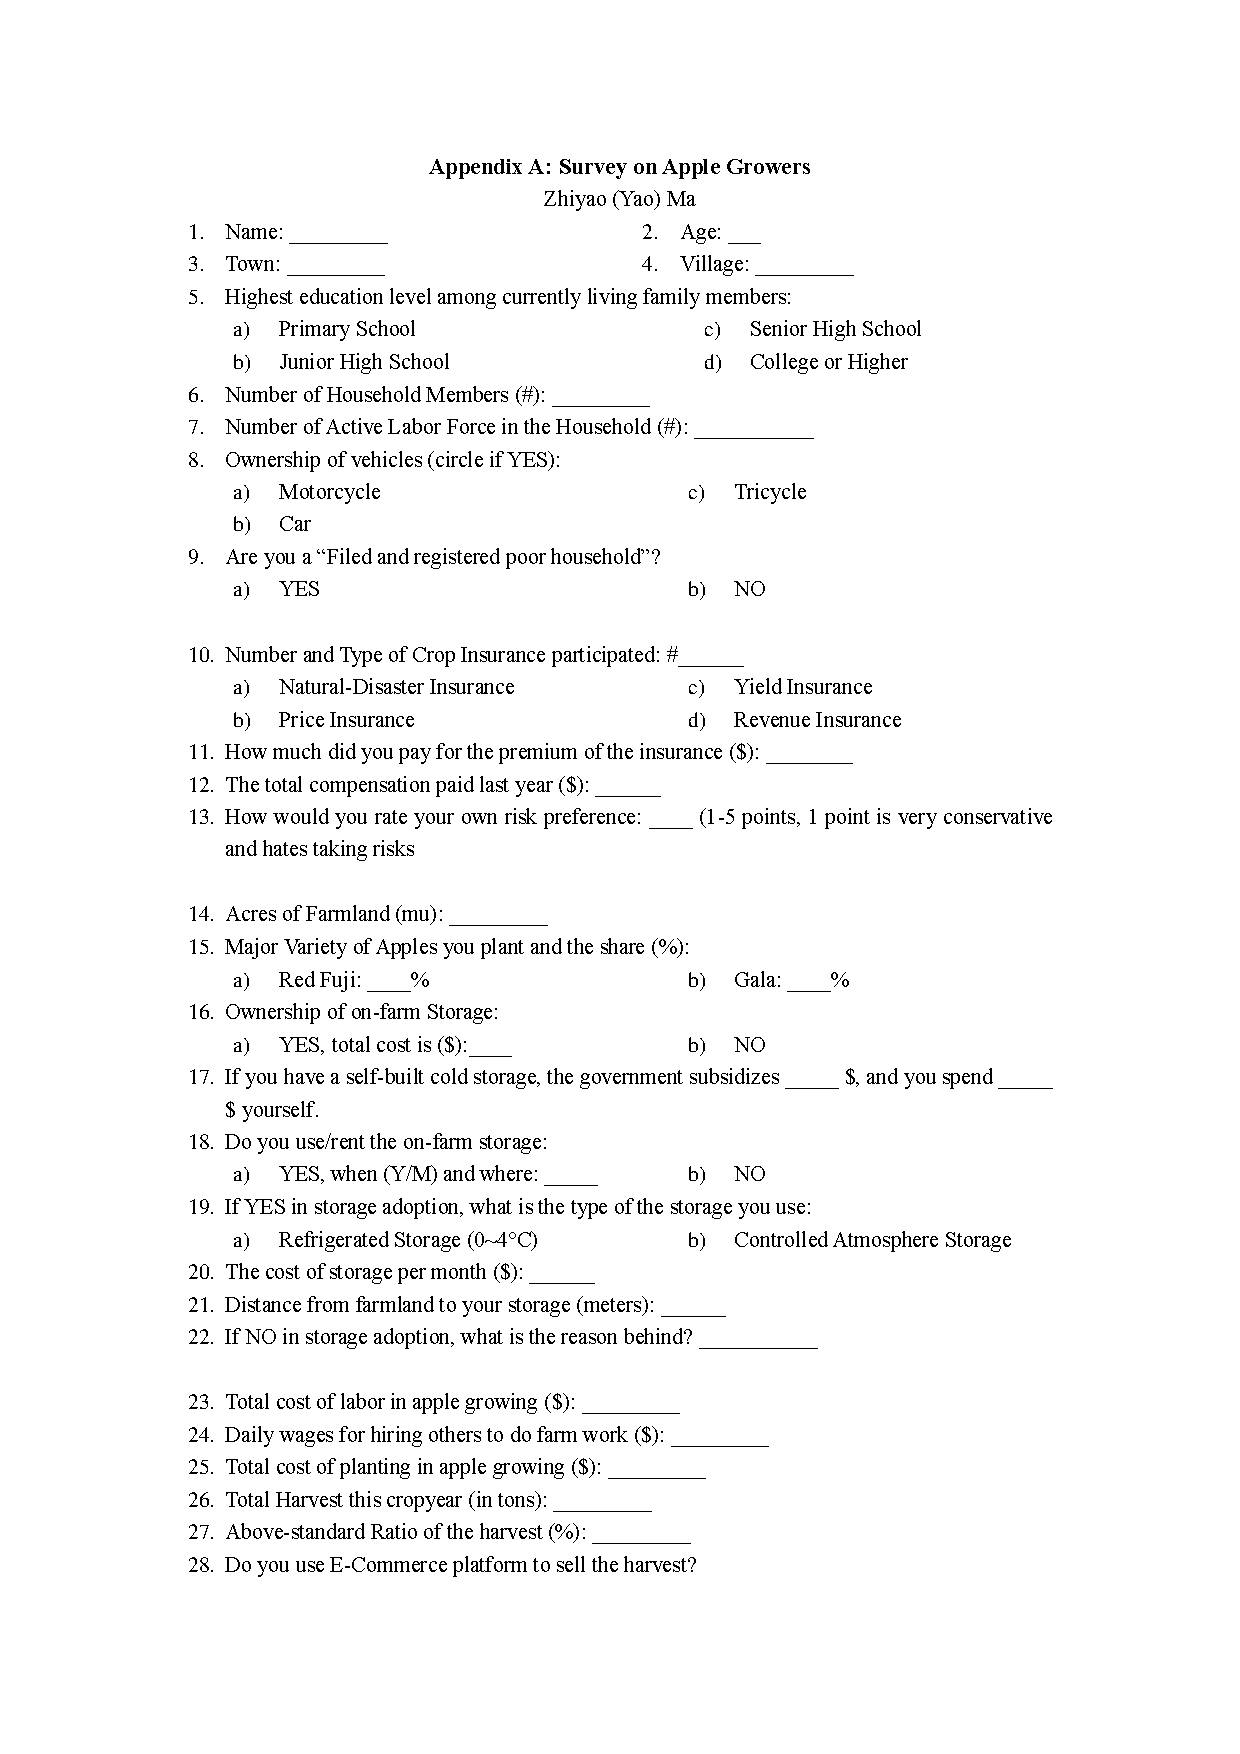
\includepdf[pages=-]{Appendix/farmers_survey.pdf}


\end{document}